
%% XXXXXX Questions used on the
%% NYSED Physics Regents Examination
%%--------------------------------------------------

%% this section contains XX problems


\begin{comment}

%% Section June1995
%%--------------------
\element{nysed}{
\begin{question}{June1995-Q02}
    A jogger accelerates at a constant rate as she travels \SI{5.0}{\meter} along a straight track from point $A$ to point $B$, as shown in the diagram below.
    \begin{center}
    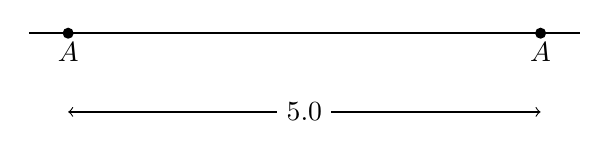
\begin{tikzpicture}
        %% runner
        %% NOTE: TODO: make vector drawing of runner
        %% ground and labels
        \draw[thick] (-3.5,0) -- (+3.5,0);
        \fill (-3,0) circle (2pt) node[anchor=north] {$A$};
        \fill (+3,0) circle (2pt) node[anchor=north] {$A$};
        \draw[<->] (-3,-1) -- (+3,-1) node[pos=0.5,anchor=center,fill=white] {\SI{5.0}{\meter}};
    \end{tikzpicture}
    \end{center}
    If her speed was \SI{2.0}{\meter\per\second} at point $A$ and will be \SI{3.0}{\meter\per\second} at point $B$,
        how long will it take her to go from $A$ to $B$?
    \begin{multicols}{2}
    \begin{choices}
        \wrongchoice{\SI{1.0}{\second}}
      \correctchoice{\SI{2.0}{\second}}
        \wrongchoice{\SI{3.3}{\second}}
        \wrongchoice{\SI{4.2}{\second}}
    \end{choices}
    \end{multicols}
\end{question}
}

\element{nysed}{
\begin{question}{June1995-Q09}
    The handle of a lawn roller is held at \ang{45} from the horizontal.
    A force, $F$, of \SI{28.0}{\newton} is applied to the handle as the roller is pushed across a level lawn,
        as shown in the diagram.
    \begin{center}
    \begin{tikzpicture}
        %% NOTE: TODO: draw tikz
    \end{tikzpicture}
    \end{center}
    What is the magnitude of the force moving the roller forward?
    \begin{multicols}{2}
    \begin{choices}
        \wrongchoice{\SI{7.00}{\newton}}
        \wrongchoice{\SI{14.0}{\newton}}
      \correctchoice{\SI{19.8}{\newton}}
        \wrongchoice{\SI{39.0}{\newton}}
    \end{choices}
    \end{multicols}
\end{question}
}

\element{nysed}{
\begin{question}{June1995-Q25}
    A neutral atom must contain equal numbers of:
    \begin{choices}
        \wrongchoice{protons and neutrons, only}
      \correctchoice{protons and electrons, only}
        \wrongchoice{electrons and neutrons, only}
        \wrongchoice{protons, neutrons and electrons}
    \end{choices}
\end{question}
}

\element{nysed}{
\begin{question}{June1995-Q31}
    Two solenoids are wound on soft iron cores and connected to batteries,
        as shown in the diagram below.
    \begin{center}
    \begin{tikzpicture}
        %% NOTE: TODO: draw tikz
    \end{tikzpicture}
    \end{center}
    When switches $S_1$ and $S_2$ are closed,
        the solenoids:
    \begin{choices}
        \wrongchoice{repel because of adjacent north poles}
        \wrongchoice{repel because of adjacent south poles}
      \correctchoice{attract because of adjacent north and south poles}
        \wrongchoice{neither attract nor repel}
    \end{choices}
\end{question}
}

\element{nysed}{
\begin{question}{June1995-Q32}
    Which diagram below best represents the magnetic field near a bar magnet?
    \begin{multicols}{2}
    \begin{choices}
        \AMCboxDimensions{down=-1.2cm}
        %% NOTE: ANS is 2
        \wrongchoice{
            \begin{tikzpicture}
                \draw[dashed,white!60!black] (-1.5,-1.5) rectangle (1.5,1.5);
                \begin{scope}[decoration={markings,mark=at position 0.5 with {\arrow{latex}}}]
                    \clip (-1.5,-1.5) rectangle (1.5,1.5);
                    \draw[thick,postaction={decorate}] (-0.66,0.12) .. controls ++(135:1) and ++(45:1) .. (0.66,0.12);
                    \draw[thick,postaction={decorate}] (-0.66,0.06) .. controls ++(135:1.5) and ++(45:1.5) .. (0.66,0.06);
                    \draw[thick,postaction={decorate}] (-0.66,-0.12) .. controls ++(225:1) and ++(315:1) .. (0.66,-0.12);
                    \draw[thick,postaction={decorate}] (-0.66,-0.06) .. controls ++(225:1.5) and ++(315:1.5) .. (0.66,-0.06);
                \end{scope}
                %% magnet
                \draw[fill=white] (-0.75,-0.25) rectangle (0.75,0.25);
                \node[anchor=west] at (-0.75,0) {S};
                \node[anchor=east] at (+0.75,0) {N};
            \end{tikzpicture}
        }
    \end{choices}
    \end{multicols}
\end{question}
}

\element{nysed}{
\begin{question}{June1995-Q34}
    The diagram below shows a piston being moved back and forth to generate a wave.
    The piston produces compression, $C$, every \SI{0.5}{\second}.
    \begin{center}
    \begin{tikzpicture}
        %% NOTE: TODO: draw tikz
    \end{tikzpicture}
    \end{center}
    The frequency of this wave is:
    \begin{multicols}{2}
    \begin{choices}
        \wrongchoice{\SI{1.0}{\hertz}}
      \correctchoice{\SI{2.0}{\hertz}}
        \wrongchoice{\SI{5.0e-1}{\hertz}}
        \wrongchoice{\SI{3.3e2}{\hertz}}
    \end{choices}
    \end{multicols}
\end{question}
}

\element{nysed}{
\begin{question}{June1995-Q35}
    The diagram below represents lines of magnetic flux within a region of space.
    \begin{center}
    \begin{tikzpicture}
        %% NOTE: TODO: draw tikz
    \end{tikzpicture}
    \end{center}
    The magnetic field strength is greatest at point:
    \begin{multicols}{4}
    \begin{choices}
        \wrongchoice{$A$}
      \correctchoice{$B$}
        \wrongchoice{$C$}
        \wrongchoice{$D$}
    \end{choices}
    \end{multicols}
\end{question}
}

\element{nysed}{
\begin{question}{June1995-Q36}
    The diagram below shows a current carrying wire located in a magnetic field which is directed toward the top of the page.
    The electromagnetic force on the wire is directed out of the page.
    \begin{center}
    \begin{tikzpicture}
        %% NOTE: TODO: draw tikz
    \end{tikzpicture}
    \end{center}
    In the wire, the electron flow is directed toward the:
    \begin{multicols}{2}
    \begin{choices}
      \correctchoice{left}
        \wrongchoice{right}
        \wrongchoice{top of the page}
        \wrongchoice{bottom of the page}
    \end{choices}
    \end{multicols}
\end{question}
}

\element{nysed}{
\begin{question}{June1995-Q40}
    Which diagram best represents the reflection of light from an irregular surface?
    \begin{multicols}{2}
    \begin{choices}
        \AMCboxDimensions{down=-1.2cm}
        %% NOTE: ANS is 3
        \wrongchoice{
            \begin{tikzpicture}
                %% NOTE: TODO: difficult tikz
            \end{tikzpicture}
        }
    \end{choices}
    \end{multicols}
\end{question}
}

\element{nysed}{
\begin{question}{June1995-Q41}
    A stationary radar gun can determine the speed of a pitched baseball by measuring the difference in frequency between incident and reflected radar waves.
    This process illustrates:
    \begin{choices}
      \correctchoice{the Doppler effect}
        \wrongchoice{standing waves}
        \wrongchoice{the critical angle}
        \wrongchoice{diffraction}
    \end{choices}
\end{question}
}

\element{nysed}{
\begin{question}{June1995-Q54}
    As the mass of a body increases,
        its gravitational force of attraction on the Earth:
    \begin{choices}
        \wrongchoice{decreases}
      \correctchoice{increases}
        \wrongchoice{remains the same}
    \end{choices}
\end{question}
}

%% Motion in a Plane
\newcommand{\nysedJuneNineteenNinetyFiveQFiftySix}{
\begin{tikzpicture}
    %% NOTE: TODO: draw tikz
\end{tikzpicture}
}

\element{nysed}{
\begin{question}{June1995-Q56}
    In the diagram below, a \SI{10}{\kilo\gram} sphere, $A$, is projected horizontally with a velocity of \SI{30}{\meter\per\second} due east from a height of \SI{20}{\meter} above level ground.
    At the same instant, a \SI{20}{\kilo\gram} sphere, $B$, is projected horizontally with a velocity of \SI{10}{\meter\per\second} due west from a height of \SI{80}{\meter} above the ground.
    [Neglect air friction]
    \begin{center}
        \nysedJuneNineteenNinetyFiveQFiftySix
    \end{center}
    %% start question
    Initially, the spheres are separated by a horizontal distance of \SI{100}{\meter}.
    What is the horizontal separation of the spheres at the end of \SI{1.5}{\second}?
    \begin{multicols}{2}
    \begin{choices}
        \wrongchoice{\SI{15}{\meter}}
        \wrongchoice{\SI{30}{\meter}}
      \correctchoice{\SI{40}{\meter}}
        \wrongchoice{\SI{45}{\meter}}
    \end{choices}
    \end{multicols}
\end{question}
}

\element{nysed}{
\begin{question}{June1995-Q57}
    In the diagram below, a \SI{10}{\kilo\gram} sphere, $A$, is projected horizontally with a velocity of \SI{30}{\meter\per\second} due east from a height of \SI{20}{\meter} above level ground.
    At the same instant, a \SI{20}{\kilo\gram} sphere, $B$, is projected horizontally with a velocity of \SI{10}{\meter\per\second} due west from a height of \SI{80}{\meter} above the ground.
    [Neglect air friction]
    \begin{center}
        \nysedJuneNineteenNinetyFiveQFiftySix
    \end{center}
    %% start question
    The magnitude of the horizontal acceleration of sphere $A$ is:
    \begin{multicols}{2}
    \begin{choices}
        %\wrongchoice{\SI{0.0}{\meter\per\second\squared}}
      \correctchoice{zero}
        \wrongchoice{\SI{2.0}{\meter\per\second\squared}}
        \wrongchoice{\SI{9.8}{\meter\per\second\squared}}
        \wrongchoice{\SI{15}{\meter\per\second\squared}}
    \end{choices}
    \end{multicols}
\end{question}
}

\element{nysed}{
\begin{question}{June1995-Q58}
    In the diagram below, a \SI{10}{\kilo\gram} sphere, $A$, is projected horizontally with a velocity of \SI{30}{\meter\per\second} due east from a height of \SI{20}{\meter} above level ground.
    At the same instant, a \SI{20}{\kilo\gram} sphere, $B$, is projected horizontally with a velocity of \SI{10}{\meter\per\second} due west from a height of \SI{80}{\meter} above the ground.
    [Neglect air friction]
    \begin{center}
        \nysedJuneNineteenNinetyFiveQFiftySix
    \end{center}
    %% start question
    Compared to the vertical acceleration of sphere $A$,
        the vertical acceleration of sphere $B$:
    \begin{multicols}{2}
    \begin{choices}
      \correctchoice{the same}
        \wrongchoice{twice as great}
        \wrongchoice{one-half as great}
        \wrongchoice{four-times as great}
    \end{choices}
    \end{multicols}
\end{question}
}


%% Section June1994
%%--------------------
\element{nysed}{
\begin{question}{June1994-Q03}
    As shown in the diagram below, an astronaut on the Moon is holding a baseball and a balloon.
    The astronaut releases both objects at the same time.
    \begin{center}
    \begin{tikzpicture}
        %% NOTE: TODO:
    \end{tikzpicture}
    \end{center}
    What does the astronaut observe?
    [Note: The Moon has no atmosphere]
    \begin{choices}
        \wrongchoice{The baseball falls slower than the balloon.}
        \wrongchoice{The baseball falls faster than the balloon.}
      \correctchoice{The baseball and balloon fall at the same rate.}
        \wrongchoice{The baseball and balloon remain suspended and do not fall.}
    \end{choices}
\end{question}
}

\element{nysed}{
\begin{question}{June1994-Q08}
    The graph below shows speed as a function of time for four cars, $A$, $B$, $C$, and $D$, in straight-line motion.
    \begin{center}
    \begin{tikzpicture}
        \begin{axis}[
            axis y line=left,
            axis x line=bottom,
            axis line style={->},
            xlabel={time},
            x unit=\si{\second},
            xtick={0,2,4,6},
            minor x tick num=1,
            ylabel={speed},
            y unit=\si{\meter\per\second},
            ytick={0,5,10,15},
            minor x tick num=4,
            xmin=0,xmax=6,
            ymin=0,ymax=15,
            width=1.0\columnwidth,
            height=0.618\columnwidth,
            very thin,
        ]
        %% NOTE: draw car function
        \draw[line width=1pt] (axis cs:0,10) -- (axis cs:6,10) node[pos=0.1,anchor=south] {Car $A$};
        \draw[dashed,thick] (axis cs:0,7) -- (axis cs:6,12) node[pos=0.1,anchor=south,rotate=10] {Car $B$};
        \draw[dashed,thick] (axis cs:0,0) to[out=70,in=190] (axis cs:1.5,5) -- (axis cs:6,5.5) node[pos=0.2,anchor=south] {Car $C$};
        \draw[dashed,thick] (axis cs:0,0) -- (axis cs:3,0.5) to[out=10,in=240] (axis cs:4.5,4) to[out=60,in=230] (axis cs: 6,9) node[pos=0.5,anchor=south] {Car $D$};
        \end{axis}
    \end{tikzpicture}
    \end{center}
    Which car experiences the greatest average acceleration during this \SI{6.0}{\second} interval?
    \begin{multicols}{2}
    \begin{choices}[o]
        \wrongchoice{car $A$}
        \wrongchoice{car $B$}
        \wrongchoice{car $C$}
      \correctchoice{car $D$}
    \end{choices}
    \end{multicols}
\end{question}
}

\newcommand{\nysedJuneNineteenNinetyFourQNine}{
%% NOTE: TODO: draw picture
\begin{tikzpicture}
    %% ground
    \draw[line width=1pt] (-4,0) -- (4,0);
    %% speed limit
    \node[draw,anchor=center,text width=4em,text centered] (S) at (3,2) {Speed Limit \SI{25}{\meter\per\second}};
    \draw[black,line width=2.0pt] (S.south) -- ++(270:2);
    \draw[white,line width=1.5pt] (S.south) -- ++(270:2);
    %% police car
    %% tree
\end{tikzpicture}
}

\element{nysed}{
\begin{question}{June1994-Q09}
    A car is traveling at a constant speed of \SI{14}{\meter\per\second} along a straight highway.
    A tree and a speed limit sign are beside the highway.
    As it passes the tree, the car starts to accelerate.
    The car is accelerated uniformly at \SI{2.0}{\meter\per\second\squared} until it reaches the speed limit sign,
        \SI{5.0}{\second} later.
    \begin{center}
        \nysedJuneNineteenNinetyFourQNine
    \end{center}
    When the car reaches the sign, the car's speed is:
    \begin{choices}
      \correctchoice{less than the speed limit}
        \wrongchoice{greater than the speed limit}
        \wrongchoice{equal to the speed limit}
    \end{choices}
\end{question}
}

\element{nysed}{
\begin{question}{June1994-Q10}
    A car is traveling at a constant speed of \SI{14}{\meter\per\second} along a straight highway.
    A tree and a speed limit sign are beside the highway.
    As it passes the tree, the car starts to accelerate.
    The car is accelerated uniformly at \SI{2.0}{\meter\per\second\squared} until it reaches the speed limit sign,
        \SI{5.0}{\second} later.
    \begin{center}
        \nysedJuneNineteenNinetyFourQNine
    \end{center}
    What is the distance between the tree and the sign?
    \begin{multicols}{2}
    \begin{choices}
        \wrongchoice{\SI{12}{\meter}}
        \wrongchoice{\SI{25}{\meter}}
        \wrongchoice{\SI{70}{\meter}}
      \correctchoice{\SI{95}{\meter}}
    \end{choices}
    \end{multicols}
\end{question}
}

\element{nysed}{
\begin{question}{June1994-Q17}
    A student pulls a block \SI{3.0}{\meter} along a horizontal surface at constant velocity.
    The diagram below shows the components of the force exerted on the block by the student.
    \begin{center}
    \begin{tikzpicture}
        %% NOTE: TODO: draw
    \end{tikzpicture}
    \end{center}
    How much work is done against friction?
    \begin{multicols}{2}
    \begin{choices}
        \wrongchoice{\SI{18}{\joule}}
      \correctchoice{\SI{24}{\joule}}
        \wrongchoice{\SI{30}{\joule}}
        \wrongchoice{\SI{42}{\joule}}
    \end{choices}
    \end{multicols}
\end{question}
}

\element{nysed}{
\begin{question}{June1994-Q18}
    The diagram below shows a \SI{1.0e3}{\newton} crate to be lifted at constant speed from the ground to a loading dock \SI{1.5}{\meter} high in \SI{5.0}{\second}.
    \begin{center}
    \begin{tikzpicture}
        %% Ground
        \draw (-4,0) -- (4,0);
        \node[anchor=north,minimum width=8cm,pattern=north east lines] at (0,0) {};
        %% This end up
        \node[draw,anchor=south,text width=5em,text centered] at (-2.5,0) {{\footnotesize This End Up} \SI{1.0e3}{\newton}};
        \node[draw,anchor=south,fill=white!90!black,minimum size=2.5cm] (B) at (+1.5,0) {};
        \node[anchor=south] at (B.south) {Loading Dock};
        %% 1.5 meter
        \draw[<->] (3.66,0) -- (3.66,2.5) node[pos=0.5,anchor=center,fill=white] {\SI{1.5}{\meter}};
    \end{tikzpicture}
    \end{center}
    What power is required to lift the crate?
    \begin{multicols}{2}
    \begin{choices}
        \wrongchoice{\SI{1.5e3}{\watt}}
        \wrongchoice{\SI{2.0e2}{\watt}}
      \correctchoice{\SI{3.0e2}{\watt}}
        \wrongchoice{\SI{7.5e3}{\watt}}
    \end{choices}
    \end{multicols}
\end{question}
}

\element{nysed}{
\begin{question}{June1994-Q36}
    An accelerating particle that does \emph{not} generate electromagnetic waves could be:
    \begin{multicols}{2}
    \begin{choices}
      \correctchoice{a neutron}
        \wrongchoice{a proton}
        \wrongchoice{an electron}
        \wrongchoice{an alpha particle}
    \end{choices}
    \end{multicols}
\end{question}
}

\newcommand{\nysedJuneNineteenNinetyFourQThirtyNine}{
\begin{tikzpicture}
    %% NOTE: TODO: draw diagram
\end{tikzpicture}
}

\element{nysed}{
\begin{question}{June1994-Q39}
    the diagram below shows a parked police car with a siren on top.
    The siren is producing a sound with a frequency of \SI{680}{\hertz},
        which travel first through point $A$ and then through point $B$, as shown.
    The speed of the sound is \SI{340}{\meter\per\second}.
    \begin{center}
        \nysedJuneNineteenNinetyFourQThirtyNine
    \end{center}
    If the sound waves are in phase at point $A$ and $B$,
        the distance between the points could be:
    \begin{multicols}{4}
    \begin{choices}
      \correctchoice{$\lambda$}
        \wrongchoice{$\dfrac{\lambda}{2}$}
        \wrongchoice{$\dfrac{3\lambda}{2}$}
        \wrongchoice{$\dfrac{\lambda}{4}$}
    \end{choices}
    \end{multicols}
\end{question}
}

\element{nysed}{
\begin{question}{June1994-Q40}
    the diagram below shows a parked police car with a siren on top.
    The siren is producing a sound with a frequency of \SI{680}{\hertz},
        which travel first through point $A$ and then through point $B$, as shown.
    The speed of the sound is \SI{340}{\meter\per\second}.
    \begin{center}
        \nysedJuneNineteenNinetyFourQThirtyNine
    \end{center}
    What is the wavelength of the sound produced by the car's siren?
    \begin{multicols}{2}
    \begin{choices}
      \correctchoice{\SI{0.50}{\meter}}
        \wrongchoice{\SI{2.0}{\meter}}
        \wrongchoice{\SI{2.3e5}{\meter}}
        \wrongchoice{\SI{2.3e-6}{\meter}}
    \end{choices}
    \end{multicols}
\end{question}
}

\element{nysed}{
\begin{question}{June1994-Q41}
    the diagram below shows a parked police car with a siren on top.
    The siren is producing a sound with a frequency of \SI{680}{\hertz},
        which travel first through point $A$ and then through point $B$, as shown.
    The speed of the sound is \SI{340}{\meter\per\second}.
    \begin{center}
        \nysedJuneNineteenNinetyFourQThirtyNine
    \end{center}
    If the car were to accelerate toward point $A$,
        the frequency of the sound heard by an observer at point $A$ would:
    \begin{choices}
        \wrongchoice{decrease}
      \correctchoice{increase}
        \wrongchoice{remain the same}
    \end{choices}
\end{question}
}

\element{nysed}{
\begin{question}{June1994-Q50}
    An x-ray photon collides with an electron in an atom,
        ejecting the electron and emitted another photon.
    During the collision, there is conservation of:
    \begin{choices}
        \wrongchoice{momentum, only}
        \wrongchoice{energy, only}
      \correctchoice{both momentum and energy}
        \wrongchoice{neither momentum nor energy}
    \end{choices}
\end{question}
}

\element{nysed}{
\begin{question}{June1994-Q55}
    A car is driven from Buffalo to Albany and on to New York City,
        as shown in the diagram below.
    Compared to the magnitude of the car's total displacement,
        the distance driven is:
    \begin{multicols}{3}
    \begin{choices}
        \wrongchoice{shorter}
      \correctchoice{longer}
        \wrongchoice{the same}
    \end{choices}
    \end{multicols}
\end{question}
}

%% Motion in a plane
\newcommand{\nysedJuneNineteenNinetyFourQFiftySix}{
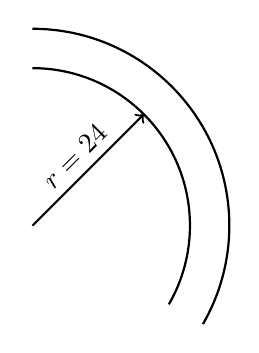
\begin{tikzpicture}
    %% NOTE: TODO: draw tikz
    %% Track
    \draw[thick] (90:2) arc (90:-30:2);
    \draw[thick] (90:2.5) arc (90:-30:2.5);
    %% radius
    \draw[thick,->] (0,0) -- (45:2) node[pos=0.5,anchor=south,rotate=45] {$r=\SI{24}{\meter}$};
    %% vehicle
    \node[minimum size=1ex] at (45:2.25) {};
\end{tikzpicture}
}

\element{nysed}{
\begin{question}{June1994-Q56}
    A vehicle travels at a constant speed of \SI{6.0}{\meter\per\second} around a horizontal circular curve with a radius of \SI{24}{\meter}.
    The mass of the vehicle is \SI{4.4e3}{\kilo\gram}.
    An icy patch is located at $P$ on the curve.
    \begin{center}
        \nysedJuneNineteenNinetyFourQFiftySix
    \end{center}
    What is the magnitude of the frictional force that keeps the vehicle on its circular path?
    \begin{multicols}{2}
    \begin{choices}
        \wrongchoice{\SI{1.1e3}{\newton}}
      \correctchoice{\SI{6.6e3}{\newton}}
        \wrongchoice{\SI{4.3e4}{\newton}}
        \wrongchoice{\SI{6.5e4}{\newton}}
    \end{choices}
    \end{multicols}
\end{question}
}

\element{nysed}{
\begin{question}{June1994-Q57}
    A vehicle travels at a constant speed of \SI{6.0}{\meter\per\second} around a horizontal circular curve with a radius of \SI{24}{\meter}.
    The mass of the vehicle is \SI{4.4e3}{\kilo\gram}.
    An icy patch is located at $P$ on the curve.
    \begin{center}
        \nysedJuneNineteenNinetyFourQFiftySix
    \end{center}
    On the icy patch of pavement,
        the frictional force on the vehicle is zero.
    Which arrow best represents the direction of the vehicle's velocity when its reaches icy patch $P$?
    \begin{multicols}{2}
    \begin{choices}
        \AMCboxDimensions{down=-1cm}
        \wrongchoice{
            \begin{tikzpicture}
                \draw[dashed,white!60!black] (-1.5,-1.5) rectangle (1.5,1.5);
                \draw[thick,->] (0,0.5) -- (1,0.5);
            \end{tikzpicture}
        }
        \wrongchoice{
            \begin{tikzpicture}
                \draw[dashed,white!60!black] (-1.5,-1.5) rectangle (1.5,1.5);
                \draw[thick,->] (1,0.5) -- (0,0.5);
            \end{tikzpicture}
        }
        \wrongchoice{
            \begin{tikzpicture}
                \draw[dashed,white!60!black] (-1.5,-1.5) rectangle (1.5,1.5);
                \draw[thick,->] (0.5,0) -- (0.5,1);
            \end{tikzpicture}
        }
        %% ANS is 4
        \correctchoice{
            \begin{tikzpicture}
                \draw[dashed,white!60!black] (-1.5,-1.5) rectangle (1.5,1.5);
                \draw[thick,->] (0.5,1) -- (0.5,0);
            \end{tikzpicture}
        }
    \end{choices}
    \end{multicols}
\end{question}
}

\newcommand{\nysedJuneNineteenNinetyFourQFiftyEight}{
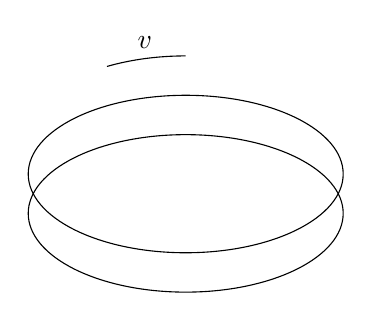
\begin{tikzpicture}
    %% NOTE: TODO: draw tikz
    \draw (0,0) circle (2cm and 1cm);
    \draw (0,0.5) circle (2cm and 1cm);
    %% velocity
    \draw (0,2) arc(90:120:2cm and 1cm) node[pos=0.5,anchor=south] {$v$};
\end{tikzpicture}
}

\element{nysed}{
\begin{question}{June1994-Q58}
    A \SI{60}{\kilo\gram} adult and a \SI{30}{\kilo\gram} child are passengers on a rotor ride at an amusement park.
    When the rotating hollow cylinder reaches a certain constant speed, $v$,
        the floor moves downward.
    Both passengers stay ``pinned'' against the wall of the rotor, as shown in the diagram below.
    \begin{center}
        \nysedJuneNineteenNinetyFourQFiftyEight
    \end{center}
    The magnitude  of the frictional force between the adult and the wall of the spinning rotor is $F$.
    What is the magnitude of the frictional force between the child and the wall of the spinning rotor?
    \begin{multicols}{4}
    \begin{choices}
        \wrongchoice{$F$}
        \wrongchoice{$2F$}
      \correctchoice{$\dfrac{F}{2}$}
        \wrongchoice{$\dfrac{F}{4}$}
    \end{choices}
    \end{multicols}
\end{question}
}

\element{nysed}{
\begin{question}{June1994-Q59}
    A \SI{60}{\kilo\gram} adult and a \SI{30}{\kilo\gram} child are passengers on a rotor ride at an amusement park.
    When the rotating hollow cylinder reaches a certain constant speed, $v$,
        the floor moves downward.
    Both passengers stay ``pinned'' against the wall of the rotor, as shown in the diagram below.
    \begin{center}
        \nysedJuneNineteenNinetyFourQFiftyEight
    \end{center}
    Compared to the magnitude of the acceleration of the adult,
        the magnitude of the acceleration of the child is:
    \begin{multicols}{3}
    \begin{choices}
        \wrongchoice{less}
        \wrongchoice{greater}
      \correctchoice{the same}
    \end{choices}
    \end{multicols}
\end{question}
}

\element{nysed}{
\begin{question}{June1994-Q60}
    A satellite is moving at constant speed in a circular orbit about the Earth,
        as shown in the diagram below.
    \begin{center}
    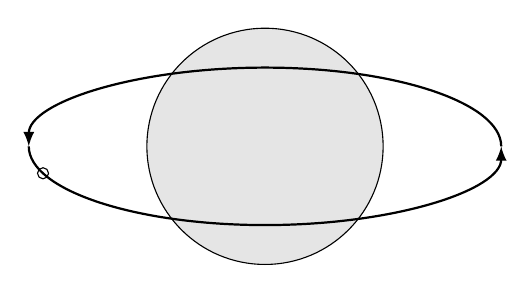
\begin{tikzpicture}
        %% NOTE: TODO: draw tikz
        %% Earth
        \draw[fill=white!90!black] (0,0) circle (1.5);
        %% orbit
        \draw[thick,-latex] (-3,0) arc (180:360:3cm and 1cm);
        \draw[thick,-latex] (+3,0) arc (0:180:3cm and 1cm);
        %% Satellite
        \draw ({3*cos(200)},{1*sin(200)}) circle (2pt);
    \end{tikzpicture}
    \end{center}
    The net force acting on the satellite is directed toward point:
    \begin{multicols}{4}
    \begin{choices}[o]
        \wrongchoice{$A$}
      \correctchoice{$B$}
        \wrongchoice{$C$}
        \wrongchoice{$D$}
    \end{choices}
    \end{multicols}
\end{question}
}

\element{nysed}{
\begin{question}{June1994-Q61}
    Which diagram best represents the orbit of the planet Pluto around the Sun?
    \begin{multicols}{2}
    \begin{choices}
        \AMCboxDimensions{down=-1cm}
        %% NOTE: ANS is 3
        \wrongchoice{
            \begin{tikzpicture}
            \end{tikzpicture}
        }
    \end{choices}
    \end{multicols}
\end{question}
}

\newcommand{\nysedJuneNineteenNinetyFourQSixtyTwo}{
\begin{tikzpicture}
    %% NOTE: TODO: draw tikz
\end{tikzpicture}
}

\element{nysed}{
\begin{question}{June1994-Q62}
    The diagram below shows a ball projected horizontally with an initial velocity of \SI{20}{\meter\per\second}, off a cliff \SI{100}{\meter} high.
    [Neglect air resistance.]
    \begin{center}
        \nysedJuneNineteenNinetyFourQSixtyTwo
    \end{center}
    How many seconds does the ball take to reach the ground?
    \begin{multicols}{2}
    \begin{choices}
      \correctchoice{\SI{4.5}{\second}}
        \wrongchoice{\SI{20}{\second}}
        \wrongchoice{\SI{9.8}{\second}}
        \wrongchoice{\SI{2.0}{\second}}
    \end{choices}
    \end{multicols}
\end{question}
}

\element{nysed}{
\begin{question}{June1994-Q63}
    The diagram below shows a ball projected horizontally with an initial velocity of \SI{20}{\meter\per\second}, off a cliff \SI{100}{\meter} high.
    [Neglect air resistance.]
    \begin{center}
        \nysedJuneNineteenNinetyFourQSixtyTwo
    \end{center}
    During the flight of the ball,
        what is the direction of its acceleration?
    \begin{multicols}{2}
    \begin{choices}
      \correctchoice{downward}
        \wrongchoice{upward}
        \wrongchoice{westward}
        \wrongchoice{eastward}
    \end{choices}
    \end{multicols}
\end{question}
}

\element{nysed}{
\begin{question}{June1994-Q64}
    A projectile is fired at an angle of \ang{53} to the horizontal with a speed of \SI{80}{\meter\per\second}.
    What is the vertical component of the projectile's initial velocity?
    \begin{multicols}{2}
    \begin{choices}
        \wrongchoice{\SI{130}{\meter\per\second}}
        \wrongchoice{\SI{100}{\meter\per\second}}
      \correctchoice{\SI{64}{\meter\per\second}}
        \wrongchoice{\SI{48}{\meter\per\second}}
    \end{choices}
    \end{multicols}
\end{question}
}

\element{nysed}{
\begin{question}{June1994-Q65}
    As the distance between the Moon and Earth increases,
        the Moon's orbital speed:
    \begin{choices}
      \correctchoice{increases}
        \wrongchoice{decreases}
        \wrongchoice{remains the same}
    \end{choices}
\end{question}
}

%% Electromagnetic application
\element{nysed}{
\begin{question}{June1994-Q76}
    A beam of particles is produced in a cathode-ray tube.
    The beam may be deflected by a magnetic field because each particle in the beam:
    \begin{choices}
      \correctchoice{possesses a charge}
        \wrongchoice{is at rest}
        \wrongchoice{has a rest mass greater than \SI{9.1e-31}{\kilo\gram}}
        \wrongchoice{has a speed of \SI{3.0e8}{\meter\per\second}}
    \end{choices}
\end{question}
}

\element{nysed}{
\begin{question}{June1994-Q77}
    Which device does \emph{not} operate by means of torque exerted on a current-carrying loop of wire in a magnetic field?
    \begin{multicols}{2}
    \begin{choices}
        \wrongchoice{ammeter}
        \wrongchoice{electric motor}
      \correctchoice{transformer}
        \wrongchoice{voltmeter}
    \end{choices}
    \end{multicols}
\end{question}
}

\newcommand{\nysedJuneNineteenNinetyFourQSeventyEight}{
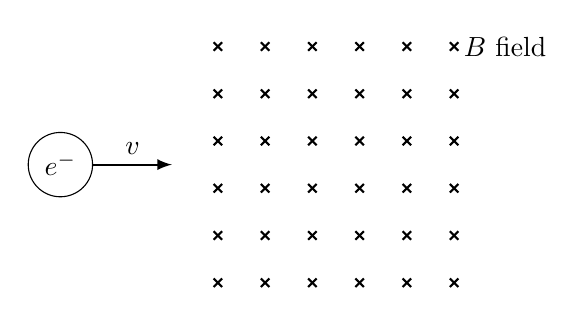
\begin{tikzpicture}
    %% B field
    \node[anchor=west] at (3,3) {$B$ field};
    \foreach \x in {0,6,...,30}
        \foreach \y in {0,6,...,30}
            \foreach \z in {45,135,225,315}
                \draw[thick] (\x mm,\y mm) -- ++(\z:0.5ex);
    %% electron
    \node[circle,draw,anchor=center] (A) at (-2,1.5) {$e^-$};
    \draw[thick,-latex] (A.east) -- ++(0:1cm) node[pos=0.5,anchor=south] {$v$};
\end{tikzpicture}
}

\element{nysed}{
\begin{question}{June1994-Q78}
    The diagram below represents an electron about to enter uniform magnetic field $B$.
    The velocity of the electron, $v$, is \SI{6.0e7}{\meter\per\second} to the right.
    The flux density of the magnetic field is \SI{4.0e-2}{\tesla},
        directed into the page.
    \begin{center}
        \nysedJuneNineteenNinetyFourQSeventyEight
    \end{center}
    When the electron first enters the magnetic field,
        the electron experiences a magnetic force directed toward the:
    \begin{multicols}{2}
    \begin{choices}
        \wrongchoice{top of the page}
      \correctchoice{bottom of the page}
        \wrongchoice{left of the page}
        \wrongchoice{right of the page}
    \end{choices}
    \end{multicols}
\end{question}
}

\element{nysed}{
\begin{question}{June1994-Q79}
    The diagram below represents an electron about to enter uniform magnetic field $B$.
    The velocity of the electron, $v$, is \SI{6.0e7}{\meter\per\second} to the right.
    The flux density of the magnetic field is \SI{4.0e-2}{\tesla},
        directed into the page.
    \begin{center}
        \nysedJuneNineteenNinetyFourQSeventyEight
    \end{center}
    The magnitude of the magnetic force acting on the electron in the field is approximately:
    \begin{multicols}{2}
    \begin{choices}
        \wrongchoice{\SI{2.4e-11}{\newton}}
      \correctchoice{\SI{3.8e-13}{\newton}}
        \wrongchoice{\SI{1.6e-18}{\newton}}
        \wrongchoice{\SI{2.2e-25}{\newton}}
    \end{choices}
    \end{multicols}
\end{question}
}

\element{nysed}{
\begin{question}{June1994-Q80}
    In the diagram below, an electron moving with speed $v$ enters the space between two oppositely charged parallel plates.
    \begin{center}
    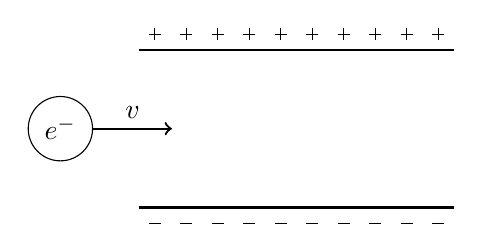
\begin{tikzpicture}
        %% electron
        \node[circle,draw] (A) at (-1,1)  {$e^-$};
        \draw[thick,->] (A.east) -- ++(0:1) node[pos=0.5,anchor=south] {$v$};
        %% Upper Plate
        \draw[thick] (0,2) -- (4,2);
        \foreach \x in {2,6,...,38}
            \foreach \y in {0,90,180,270}
                \draw (\x mm,2.2) -- ++(\y:0.5ex);
        %% Lower Plate
        \draw[thick] (0,0) -- (4,0);
        \foreach \x in {2,6,...,38}
            \foreach \y in {0,180}
                \draw (\x mm,-0.2) -- ++(\y:0.5ex);
    \end{tikzpicture}
    \end{center}
    Which diagram best represents the path the electron follows as it passes between the plates?
    \begin{multicols}{2}
    \begin{choices}
        \AMCboxDimensions{down=-1cm}
        \wrongchoice{
            \begin{tikzpicture}
                \draw[dashed,white!60!black] (-1.5,-1.5) rectangle (1.5,1.5);
                %\path[thick,decoration={markings,mark=at position 0.5 with {\arrow{latex}}},decorate}] (-1.5,0) -- (1.5,0);
            \end{tikzpicture}
        }
        \wrongchoice{
            \begin{tikzpicture}
                \draw[dashed,white!60!black] (-1.5,-1.5) rectangle (1.5,1.5);
                %\path[thick,decoration={markings,mark=at position 0.5 with {\arrow{latex}}},decorate}] (-1,1) arc(90:-90:1);
            \end{tikzpicture}
        }
        %% NOTE: ANS is 3
        \wrongchoice{
            \begin{tikzpicture}
                \draw[dashed,white!60!black] (-1.5,-1.5) rectangle (1.5,1.5);
                %\path[thick,decoration={markings,mark=at position 0.5 with {\arrow{latex}}},decorate}] (-1.5,-0.5) to[out=0,in=200] (1.5,0.5);
            \end{tikzpicture}
        }
        \wrongchoice{
            \begin{tikzpicture}
                \draw[dashed,white!60!black] (-1.5,-1.5) rectangle (1.5,1.5);
                %\path[thick,decoration={markings,mark=at position 0.5 with {\arrow{latex}}},decorate}] (-1.5,-0.5) to[out=0,in=160] (1.5,-0.5);
            \end{tikzpicture}
        }
    \end{choices}
    \end{multicols}
\end{question}
}

\element{nysed}{
\begin{question}{June1994-Q81}
    After Millikan performed his oil drop experiment, he concluded that:
    \begin{choices}
      \correctchoice{there is a minimum amount of charge that particles can acquire}
        \wrongchoice{oil drops exhibit gravitational attraction for other other drops}
        \wrongchoice{oil drops are largely empty space}
        \wrongchoice{there is a minimum amount of mass that particles can acquire}
    \end{choices}
\end{question}
}

\element{nysed}{
\begin{question}{June1994-Q82}
    When a \SI{12}{\volt} potential difference is applied to the primary coil of a transformer,
        an \SI{8}{\volt} potential difference is induced in the secondary coil.
    If the primary coil has 24 turns, how many turns does the secondary coil have?
    [Assume \SI{100}{\percent} efficiency.]
    \begin{multicols}{4}
    \begin{choices}
        \wrongchoice{36}
      \correctchoice{16}
        \wrongchoice{3}
        \wrongchoice{4}
    \end{choices}
    \end{multicols}
\end{question}
}

\newcommand{\nysedJuneNineteenNinetyFourQEightyThree}{
\begin{tikzpicture}
    %% NOTE: TODO: draw tikz
\end{tikzpicture}
}

\element{nysed}{
\begin{question}{June1994-Q83}
    The diagram below shows a loop of wire being rotated at a constant rate about an axis in a uniform magnetic field.
    \begin{center}
        \nysedJuneNineteenNinetyFourQEightyThree
    \end{center}
    Which graph best represents the relationship between induced potential difference across the ends of the loop and time,
        for one complete rotation?
    \begin{multicols}{2}
    \begin{choices}
        \AMCboxDimensions{down=-2.5em}
        \wrongchoice{
            \begin{tikzpicture}
                \begin{axis}[
                    axis y line=left,
                    axis x line=middle,
                    axis line style={->},
                    xlabel={time},
                    xtick=\empty,
                    ylabel={potential},
                    ytick={-1,0,1},
                    yticklabels={$-$,0,$+$},
                    xmin=0,xmax=11,
                    ymin=-1.2,ymax=1.2,
                    width=0.90\columnwidth,
                    clip=false,
                    very thin,
                ]
                \addplot[line width=1pt,mark=\empty] plot coordinates { (0,0) (1,1) (4,1) (6,-1) (9,-1) (10,0) };
                \end{axis}
            \end{tikzpicture}
        }
        \wrongchoice{
            \begin{tikzpicture}
                \begin{axis}[
                    axis y line=left,
                    axis x line=middle,
                    axis line style={->},
                    xlabel={time},
                    xtick=\empty,
                    ylabel={potential},
                    ytick={-1,0,1},
                    yticklabels={$-$,0,$+$},
                    xmin=0,xmax=11,
                    ymin=-1.2,ymax=1.2,
                    width=0.90\columnwidth,
                    clip=false,
                    very thin,
                ]
                \addplot[line width=1pt,domain=0:10] {1};
                \end{axis}
            \end{tikzpicture}
        }
        \wrongchoice{
            \begin{tikzpicture}
                \begin{axis}[
                    axis y line=left,
                    axis x line=middle,
                    axis line style={->},
                    xlabel={time},
                    x label style={anchor=north east},
                    xtick=\empty,
                    ylabel={potential},
                    ytick={-1,0,1},
                    yticklabels={$-$,0,$+$},
                    xmin=0,xmax=11,
                    ymin=-1.2,ymax=1.2,
                    width=0.90\columnwidth,
                    clip=false,
                    very thin,
                ]
                \addplot[line width=1pt,mark=\empty] plot coordinates {(0,0) (5,1) (10,0)};
                \end{axis}
            \end{tikzpicture}
        }
        %% ANS is 4
        \correctchoice{
            \begin{tikzpicture}
                \begin{axis}[
                    axis y line=left,
                    axis x line=middle,
                    axis line style={->},
                    xlabel={time},
                    xtick=\empty,
                    ylabel={potential},
                    ytick={-1,0,1},
                    yticklabels={$-$,0,$+$},
                    xmin=0,xmax=11,
                    ymin=-1.2,ymax=1.2,
                    width=0.90\columnwidth,
                    clip=false,
                    very thin,
                ]
                \addplot[line width=1pt,domain=0:10] {sin(36*x)};
                \end{axis}
            \end{tikzpicture}
        }
    \end{choices}
    \end{multicols}
\end{question}
}

\element{nysed}{
\begin{question}{June1994-Q84}
    The diagram below shows a loop of wire being rotated at a constant rate about an axis in a uniform magnetic field.
    \begin{center}
        \nysedJuneNineteenNinetyFourQEightyThree
    \end{center}
    Which procedure would enable a current to flow in the loop,
        due to the induced potential difference?
    \begin{choices}
        \wrongchoice{turning the loop in the opposite direction at the same rate of rotation}
        \wrongchoice{increasing the distance between the ends of the loop}
        \wrongchoice{connecting the ends of the loop to each other with an insulating material}
      \correctchoice{connecting the ends of the loop to each other with an conducting material}
    \end{choices}
\end{question}
}

\element{nysed}{
\begin{question}{June1994-Q85}
    The diagram below shows a loop of wire being rotated at a constant rate about an axis in a uniform magnetic field.
    \begin{center}
        \nysedJuneNineteenNinetyFourQEightyThree
    \end{center}
    As the speed of rotation of the wire loop is increased,
        the maximum electromotive force induced in the loop:
    \begin{choices}
        \wrongchoice{decreases}
      \correctchoice{increases}
        \wrongchoice{remains the same}
    \end{choices}
\end{question}
}


%% Section June1990
%%--------------------
\element{nysed}{
\begin{question}{June1990-Q15}
    A copper coin resting on a piece of cardboard is placed on a beaker as shown in the diagram below.
    When the cardboard is rapidly removed,
        the coin drops into the beaker.
    \begin{center}
    \begin{tikzpicture}
        %% NOTE: TODO: draw tikz
    \end{tikzpicture}
    \end{center}
    The two properties of the coin which best explain its fall are its weight and its:
    \begin{multicols}{2}
    \begin{choices}
        \wrongchoice{temperature}
        \wrongchoice{electrical resistance}
        \wrongchoice{volume}
      \correctchoice{inertia}
    \end{choices}
    \end{multicols}
\end{question}
}


\element{nysed}{
\begin{question}{June1990-Q25}
    Which diagram best represents the charge distribution on a neutral electroscope when a negatively charged rod is held near it?
    \begin{multicols}{2}
    \begin{choices}
        %% NOTE: ANS is 3
        \AMCboxDimensions{down=-1cm}
        \wrongchoice{
            \begin{tikzpicture}
                %% NOTE: TODO: draw tikz
            \end{tikzpicture}
        }
    \end{choices}
    \end{multicols}
\end{question}
}

\element{nysed}{
\begin{question}{June1990-Q27}
    The diagram below shows the electric field in the vicinity of two charged conducting spheres, $A$ and $B$.
    \begin{center}
    \begin{tikzpicture}
        %% NOTE: TODO: draw tikz
    \end{tikzpicture}
    \end{center}
    What is the static electric charge on each of the conducting spheres?
    \begin{choices}
        \wrongchoice{$A$ is negative and $B$ is positive}
      \correctchoice{$A$ is positive and $B$ is negative}
        \wrongchoice{Both $A$ and $B$ are positive}
        \wrongchoice{Both $A$ and $B$ are negative}
    \end{choices}
\end{question}
}



\element{nysed}{
\begin{question}{June1990-Q31}
    In which diagram below is the magnetic flux density at point $P$ greatest?
    \begin{multicols}{2}
    \begin{choices}
        %% NOTE: ANS is 4
        \AMCboxDimensions{down=-1cm}
        \wrongchoice{
            \begin{tikzpicture}
                %% NOTE: TODO: draw tikz
            \end{tikzpicture}
        }
    \end{choices}
    \end{multicols}
\end{question}
}

\element{nysed}{
\begin{question}{June1990-Q32}
    The wire loop shown below has a clockwise electron current.
    \begin{center}
    \begin{tikzpicture}
        %% NOTE: TODO: draw tikz
    \end{tikzpicture}
    \end{center}
    What is the direction of the magnetic field at point $P$?
    \begin{multicols}{2}
    \begin{choices}
        \wrongchoice{to the right}
        \wrongchoice{to the left}
        \wrongchoice{into the page}
      \correctchoice{out of the page}
    \end{choices}
    \end{multicols}
\end{question}
}



\element{nysed}{
\begin{question}{June1990-Q39}
    the diagram below represents a conductor carrying an electron current in magnetic field $B$.
    \begin{center}
    \begin{circuitikz}
        %% NOTE: TODO: draw circuit
    \end{circuitikz}
    \end{center}
    The direction of the magnetic force on the conductor is:
    \begin{choices}
      \correctchoice{into the page}
        \wrongchoice{out the page}
        \wrongchoice{toward the top of the page}
        \wrongchoice{toward the bottom of the page}
    \end{choices}
\end{question}
}

\element{nysed}{
\begin{question}{June1990-Q42}
    In the diagram below, $A$, $B$, $C$, and $D$ are points near a current carrying solenoid.
    \begin{center}
    \begin{tikzpicture}
        %% NOTE: TODO: draw tikz
    \end{tikzpicture}
    \end{center}
    Which point is closest to the north pole of the solenoid?
    \begin{multicols}{4}
    \begin{choices}
        \wrongchoice{$A$}
        \wrongchoice{$B$}
      \correctchoice{$C$}
        \wrongchoice{$D$}
    \end{choices}
    \end{multicols}
\end{question}
}

\element{nysed}{
\begin{question}{June1990-Q43}
    In the diagram below, which wave has the largest amplitude?
    \begin{center}
    \begin{tikzpicture}
        %% NOTE: TODO: draw tikz
    \end{tikzpicture}
    \end{center}
    \begin{multicols}{4}
    \begin{choices}
      \correctchoice{$A$}
        \wrongchoice{$B$}
        \wrongchoice{$C$}
        \wrongchoice{$D$}
    \end{choices}
    \end{multicols}
\end{question}
}

\element{nysed}{
\begin{question}{June1990-Q44}
    Which term describes two points on a periodic wave that are moving in the same direction and have the same displacement from their equilibrium position?
    \begin{multicols}{2}
    \begin{choices}
        \wrongchoice{dispersed}
        \wrongchoice{refracted}
        \wrongchoice{polarized}
      \correctchoice{in phase}
    \end{choices}
    \end{multicols}
\end{question}
}

\element{nysed}{
\begin{question}{June1990-Q45}
    In a vacuum, the wavelength of green light is \SI{5e-7}{\meter}.
    What is the its frequency?
    \begin{multicols}{2}
    \begin{choices}
        \wrongchoice{\SI{2e-15}{\hertz}}
        \wrongchoice{\SI{2e-14}{\hertz}}
      \correctchoice{\SI{6e14}{\hertz}}
        \wrongchoice{\SI{6e15}{\hertz}}
    \end{choices}
    \end{multicols}
\end{question}
}

\element{nysed}{
\begin{question}{June1990-Q46}
    As shown in the diagram below, a transverse wave is moving along a rope.
    \begin{center}
    \begin{tikzpicture}
        %% NOTE: TODO: draw tikz
    \end{tikzpicture}
    \end{center}
    In which direction will segment $X$ move as the wave passes through it?
    \begin{multicols}{2}
    \begin{choices}
        \wrongchoice{down, only}
        \wrongchoice{up, only}
        \wrongchoice{down, then up}
      \correctchoice{up, then down}
    \end{choices}
    \end{multicols}
\end{question}
}

\element{nysed}{
\begin{question}{June1990-Q47}
    A ray of light strikes a mirror at an angle of incidence of \ang{60}.
    What is the angle of reflection?
    \begin{multicols}{4}
    \begin{choices}
        \wrongchoice{\ang{0}}
        \wrongchoice{\ang{30}}
      \correctchoice{\ang{60}}
        \wrongchoice{\ang{90}}
    \end{choices}
    \end{multicols}
\end{question}
}

\element{nysed}{
\begin{question}{June1990-Q48}
    What is the approximate speed of light in alcohol?
    \begin{multicols}{2}
    \begin{choices}
        \wrongchoice{\SI{1.4e8}{\meter\per\second}}
      \correctchoice{\SI{2.2e8}{\meter\per\second}}
        \wrongchoice{\SI{3.0e8}{\meter\per\second}}
        \wrongchoice{\SI{4.4e8}{\meter\per\second}}
    \end{choices}
    \end{multicols}
\end{question}
}

\element{nysed}{
\begin{question}{June1990-Q50}
    In the diagram below, a ray of light enters a transparent medium from air.
    \begin{center}
    \begin{tikzpicture}
        %% NOTE: TODO: draw tikz
    \end{tikzpicture}
    \end{center}
    If angle $X$ is \ang{45} and angle $Y$ is \ang{30},
        what is the absolute index of refraction of the medium?
    \begin{multicols}{2}
    \begin{choices}
        \wrongchoice{0.667}
        \wrongchoice{0.707}
      \correctchoice{1.41}
        \wrongchoice{1.50}
    \end{choices}
    \end{multicols}
\end{question}
}

\element{nysed}{
\begin{question}{June1990-Q51}
    Which optical medium would have the smallest critical angle $(\theta_c)$ in the situation shown in the diagram?
    \begin{center}
    \begin{tikzpicture}
        %% NOTE: TODO: draw tikz
    \end{tikzpicture}
    \end{center}
    \begin{multicols}{2}
    \begin{choices}
        \wrongchoice{Lucite}
        \wrongchoice{water}
        \wrongchoice{Canada balsam}
      \correctchoice{diamond}
    \end{choices}
    \end{multicols}
\end{question}
}

\element{nysed}{
\begin{question}{June1990-Q52}
    The spreading of a wave into the regions behind an obstacle is known as:
    \begin{multicols}{2}
    \begin{choices}
        \wrongchoice{diffusion}
        \wrongchoice{dispersion}
        \wrongchoice{refraction}
      \correctchoice{diffraction}
    \end{choices}
    \end{multicols}
\end{question}
}

\element{nysed}{
\begin{question}{June1990-Q53}
    An electron in a hydrogen atom drops from the $n=3$ energy level to the $n=2$ energy level.
    The energy of the emitted photon is:
    \begin{multicols}{2}
    \begin{choices}
        \wrongchoice{\SI{1.51}{\eV}}
      \correctchoice{\SI{1.89}{\eV}}
        \wrongchoice{\SI{3.40}{\eV}}
        \wrongchoice{\SI{4.91}{\eV}}
    \end{choices}
    \end{multicols}
\end{question}
}


\element{nysed}{
\begin{question}{June1990-Q58}
    A block is at rest on an inclined plane as shown in the diagram.
    \begin{center}
    \begin{tikzpicture}
        %% NOTE: TODO: draw tikz
    \end{tikzpicture}
    \end{center}
    As the angle $\theta$ is increased, the component of the block's weight parallel to the plane:
    \begin{choices}
        \wrongchoice{decreases}
      \correctchoice{increases}
        \wrongchoice{remains the same}
    \end{choices}
\end{question}
}

\element{nysed}{
\begin{question}{June1990-Q60}
    As observed from the Earth, the light from a star is shifted toward lower frequencies.
    This is an indication that the distance between the Earth and the star is:
    \begin{choices}
        \wrongchoice{decreasing}
      \correctchoice{increasing}
        \wrongchoice{constant}
    \end{choices}
\end{question}
}

%% Motion in a Plane
\newcommand{\nysedJuneNineteenNinetyQSixtyOne}{
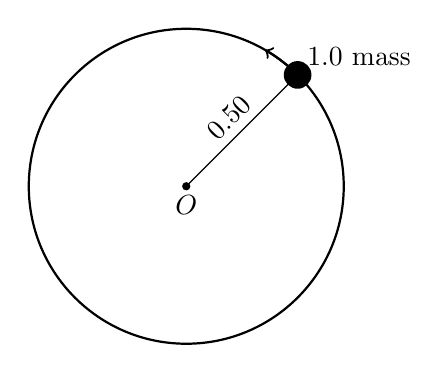
\begin{tikzpicture}
    \draw[thick] (0,0) circle (2cm);
    \draw[thick,->] (45:2) arc (45:60:2);
    \fill (0,0) circle (1.5pt) node[anchor=north] {$O$};
    \draw (0,0) -- (45:2) node[pos=0.5,anchor=south,rotate=45] {\SI{0.50}{\meter}};
    \fill (45:2) circle (5pt) node[anchor=south west] {\SI{1.0}{\kilo\gram} mass};
\end{tikzpicture}
}

\element{nysed}{
\begin{question}{June1990-Q61}
    The diagram below shows an object with a mass of \SI{1.0}{\kilo\gram} attached to a string \SI{0.50}{\meter} long.
    The object is moving at a constant speed of \SI{5.0}{\meter\per\second} in a horizontal circular path with center at point $O$.
    \begin{center}
        \nysedJuneNineteenNinetyQSixtyOne
    \end{center}
    What is the magnitude of the centripetal force acting on the object?
    \begin{multicols}{2}
    \begin{choices}
        \wrongchoice{\SI{2.5}{\newton}}
        \wrongchoice{\SI{1.0}{\newton}}
        \wrongchoice{\SI{25}{\newton}}
      \correctchoice{\SI{50}{\newton}}
    \end{choices}
    \end{multicols}
\end{question}
}

\element{nysed}{
\begin{question}{June1990-Q62}
    The diagram below shows an object with a mass of \SI{1.0}{\kilo\gram} attached to a string \SI{0.50}{\meter} long.
    The object is moving at a constant speed of \SI{5.0}{\meter\per\second} in a horizontal circular path with center at point $O$.
    \begin{center}
        \nysedJuneNineteenNinetyQSixtyOne
    \end{center}
    While the object is undergoing uniform circular motion,
        its acceleration:
    \begin{choices}
        \wrongchoice{has a magnitude of zero}
        \wrongchoice{increases in magnitude}
      \correctchoice{is directed toward the center of the circle}
        \wrongchoice{is directed away from the center of the circle}
    \end{choices}
\end{question}
}

\element{nysed}{
\begin{question}{June1990-Q63}
    The diagram below shows an object with a mass of \SI{1.0}{\kilo\gram} attached to a string \SI{0.50}{\meter} long.
    The object is moving at a constant speed of \SI{5.0}{\meter\per\second} in a horizontal circular path with center at point $O$.
    \begin{center}
        \nysedJuneNineteenNinetyQSixtyOne
    \end{center}
    If the string is cut when the object is at the position shown,
        the path the object will travel from this position will be:
    \begin{choices}
        \wrongchoice{toward the center of the circle}
        \wrongchoice{a curve away from the circle}
      \correctchoice{a straight line tangent to the circle}
    \end{choices}
\end{question}
}

\element{nysed}{
\begin{question}{June1990-Q64}
    The diagram below shows an object with a mass of \SI{1.0}{\kilo\gram} attached to a string \SI{0.50}{\meter} long.
    The object is moving at a constant speed of \SI{5.0}{\meter\per\second} in a horizontal circular path with center at point $O$.
    \begin{center}
        \nysedJuneNineteenNinetyQSixtyOne
    \end{center}
    If the string is lengthened while the speed of the object remains constant,
        the centripetal acceleration of the object will:
    \begin{choices}
      \correctchoice{decrease}
        \wrongchoice{increase}
        \wrongchoice{remain the same}
    \end{choices}
\end{question}
}

\newcommand{\nysedJuneNineteenNinetyQSixtyFive}{
\begin{tikzpicture}
    %% NOTE: draw tikz
\end{tikzpicture}
}

\element{nysed}{
\begin{question}{June1990-Q65}
    The diagram below represents a ball being kicked by a foot and rising at an angle of \ang{30} from the horizontal.
    The ball has an initial velocity of \SI{5.0}{\meter\per\second}.
    [Neglect friction.]
    \begin{center}
        \nysedJuneNineteenNinetyQSixtyFive
    \end{center}
    What is the magnitude of the horizontal component of the ball's initial velocity?
    \begin{multicols}{2}
    \begin{choices}
        \wrongchoice{\SI{2.5}{\meter\per\second}}
      \correctchoice{\SI{4.3}{\meter\per\second}}
        \wrongchoice{\SI{5.0}{\meter\per\second}}
        \wrongchoice{\SI{8.7}{\meter\per\second}}
    \end{choices}
    \end{multicols}
\end{question}
}

\element{nysed}{
\begin{question}{June1990-Q66}
    The diagram below represents a ball being kicked by a foot and rising at an angle of \ang{30} from the horizontal.
    The ball has an initial velocity of \SI{5.0}{\meter\per\second}.
    [Neglect friction.]
    \begin{center}
        \nysedJuneNineteenNinetyQSixtyFive
    \end{center}
    As the ball rises, the vertical component of its velocity
    \begin{choices}
      \correctchoice{decreases}
        \wrongchoice{increases}
        \wrongchoice{remains the same}
    \end{choices}
\end{question}
}

\element{nysed}{
\begin{question}{June1990-Q67}
    The diagram below represents a ball being kicked by a foot and rising at an angle of \ang{30} from the horizontal.
    The ball has an initial velocity of \SI{5.0}{\meter\per\second}.
    [Neglect friction.]
    \begin{center}
        \nysedJuneNineteenNinetyQSixtyFive
    \end{center}
    If the angle between the horizontal and the direction of the \SI{5.0}{\meter\per\second} velocity decreases from \ang{30} to \ang{20},
        the horizontal distance the ball travels will:
    \begin{choices}
      \correctchoice{decreases}
        \wrongchoice{increases}
        \wrongchoice{remains the same}
    \end{choices}
\end{question}
}

\element{nysed}{
\begin{question}{June1990-Q68}
    In the diagram below, $P$ represents a planet and $S$ represents the Sun.
    Which best represents the path of planet $P$ as it orbits the Sun?
    [The diagrams are not drawn to scale.]
    \begin{multicols}{2}
    \begin{choices}
        %% NOTE: ANS is 3
        \AMCboxDimensions{down=-2.5em}
        \wrongchoice{
            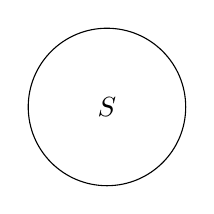
\begin{tikzpicture}
                \node[anchor=center] (S) at (0,0) {$S$};
                \draw (S) circle (1cm);
            \end{tikzpicture}
        }
    \end{choices}
    \end{multicols}
\end{question}
}

\element{nysed}{
\begin{question}{June1990-Q69}
    The Earth is closest to the Sun during January and farthest from the Sun during July.
    During which month is the gravitational potential energy of the Earth with respect to the Sun the greatest?
    \begin{multicols}{2}
    \begin{choices}
        \wrongchoice{January}
        \wrongchoice{March}
      \correctchoice{July}
        \wrongchoice{September}
    \end{choices}
    \end{multicols}
\end{question}
}

\element{nysed}{
\begin{question}{June1990-Q70}
    As the distance of a Satellite from the Earth's surface increases,
        the time the satellite takes to make one revolution around the Earth:
    \begin{choices}
        \wrongchoice{decreases}
      \correctchoice{increases}
        \wrongchoice{remains the same}
    \end{choices}
\end{question}
}


%% Electromagnetic Application
\element{nysed}{
\begin{question}{June1990-Q81}
    In the diagram below, a loop of wire is situated in uniform magnetic field $B$.
    The wire carries a constant electron current moving as shown.
    \begin{center}
    \begin{tikzpicture}
        %% NOTE: TODO: draw tikz
    \end{tikzpicture}
    \end{center}
    As viewed from position $F$,
        how will the loop initially respond to the current?
    \begin{choices}
        \wrongchoice{by sliding from $C$ to $D$}
        \wrongchoice{by sliding from $D$ to $C$}
      \correctchoice{by rotating clockwise about axis $FA$}
        \wrongchoice{by rotating counter-clockwise about axis $FA$}
    \end{choices}
\end{question}
}

\element{nysed}{
\begin{question}{June1990-Q82}
    Which statement about ammeters and voltmeters is correct?
    \begin{choices}
        \wrongchoice{The internal resistance of both meters should be low.}
      \correctchoice{Both meters should have a negligible effect on the circuit being measured.}
        \wrongchoice{The potential drop across both meters should be made as large as possible.}
        \wrongchoice{The scale range on both meters must be the same.}
    \end{choices}
\end{question}
}

\element{nysed}{
\begin{question}{June1990-Q83}
    In a practical motor,
        the coil is wound around a soft iron core.
    The purpose of the soft iron core is to:
    \begin{choices}
      \correctchoice{strengthen and concentrate the magnetic field through the coil.}
        \wrongchoice{cause the torque on the coil to remain in the same direction.}
        \wrongchoice{convert alternating current to direct current.}
        \wrongchoice{oppose the applied potential difference and reduce the current in the coil.}
    \end{choices}
\end{question}
}

\element{nysed}{
\begin{question}{June1990-Q84}
    What is the purpose of the split-ring commutator in a direct current motor?
    \begin{choices}
        \wrongchoice{to eliminate the external magnetic field.}
        \wrongchoice{to increase the current in the armature.}
      \correctchoice{to maintain the direction of rotation of the armature.}
        \wrongchoice{to decrease the induced back emf.}
    \end{choices}
\end{question}
}

\element{nysed}{
\begin{question}{June1990-Q85}
    An electron is moving at a velocity of \SI{4.0e6}{\meter\per\second} perpendicular to a magnetic field with flux density of \SI{6.0}{\tesla}.
    The magnitude of the magnetic force acting on the electron is:
    \begin{multicols}{2}
    \begin{choices}
        \wrongchoice{\SI{1.6e-13}{\newton}}
        \wrongchoice{\SI{6.4e-13}{\newton}}
      \correctchoice{\SI{3.8e-12}{\newton}}
        \wrongchoice{\SI{2.4e7}{\newton}}
    \end{choices}
    \end{multicols}
\end{question}
}

\element{nysed}{
\begin{question}{June1990-Q86}
    Which device can be used to separate isotopes of an element?
    \begin{choices}
      \correctchoice{a mass spectrometer}
        \wrongchoice{an electroscope}
        \wrongchoice{an induction coil}
        \wrongchoice{two closely spaced double slits}
    \end{choices}
\end{question}
}

\element{nysed}{
\begin{question}{June1990-Q87}
    Which could \emph{not} be accelerated using an electric field?
    \begin{multicols}{2}
    \begin{choices}
        \wrongchoice{electron}
        \wrongchoice{positron}
        \wrongchoice{alpha particle}
      \correctchoice{photon}
    \end{choices}
    \end{multicols}
\end{question}
}

\element{nysed}{
\begin{question}{June1990-Q88}
    The diagram at the right shows a wire loop rotating between magnetic poles.
    During \ang{360} of rotation from the position shown,
        the induced potential difference changes in:
    \begin{choices}
        \wrongchoice{direction, only}
        \wrongchoice{magnitude, only}
      \correctchoice{both magnitude and direction}
        \wrongchoice{neither magnitude nor direction}
    \end{choices}
\end{question}
}

\element{nysed}{
\begin{question}{June1990-Q89}
    A transformer has 150 turns of wire in the primary coil and \num{1 200} turns of wire in the secondary coil.
    The potential difference across the primary is \SI{110}{\volt}.
    What is the potential difference induced across the secondary coil?
    \begin{multicols}{2}
    \begin{choices}
        \wrongchoice{\SI{14}{\volt}}
        \wrongchoice{\SI{110}{\volt}}
        \wrongchoice{\SI{150}{\volt}}
      \correctchoice{\SI{880}{\volt}}
    \end{choices}
    \end{multicols}
\end{question}
}

\element{nysed}{
\begin{question}{June1990-Q90}
    Which term best describes the light generated by a laser?
    \begin{multicols}{2}
    \begin{choices}
        \wrongchoice{diffused}
      \correctchoice{coherent}
        \wrongchoice{dispersive}
        \wrongchoice{longitudinal}
    \end{choices}
    \end{multicols}
\end{question}
}

%% Geometric Optics
\newcommand{\nysedJuneNineteenNinetyQNinetyOne}{
\begin{tikzpicture}
    %% NOTE: TODO: draw tikz
\end{tikzpicture}
}

\element{nysed}{
\begin{question}{June1990-Q91}
    The diagram below shows four rays of light from object $AB$ incident upon a spherical mirror whose focal length is \SI{0.04}{\meter}.
    Point $F$ is the principal focus of the mirror, point $C$ is the center of curvature,
        and point $O$ is located on the principal axis.
    \begin{center}
        \nysedJuneNineteenNinetyQNinetyOne
    \end{center}
    Which ray of light will pas through $F$ after it is reflected from the mirror?
    \begin{multicols}{4}
    \begin{choices}
        \wrongchoice{1}
      \correctchoice{2}
        \wrongchoice{3}
        \wrongchoice{4}
    \end{choices}
    \end{multicols}
\end{question}
}

\element{nysed}{
\begin{question}{June1990-Q92}
    The diagram below shows four rays of light from object $AB$ incident upon a spherical mirror whose focal length is \SI{0.04}{\meter}.
    Point $F$ is the principal focus of the mirror, point $C$ is the center of curvature,
        and point $O$ is located on the principal axis.
    \begin{center}
        \nysedJuneNineteenNinetyQNinetyOne
    \end{center}
    If object $AB$ is located \SI{0.05}{\meter} from point $O$,
        its image will be located:
    \begin{choices}
      \correctchoice{farther from mirror than $C$}
        \wrongchoice{between $C$ and $F$}
        \wrongchoice{between $F$ and the mirror}
        \wrongchoice{behind the mirror}
    \end{choices}
\end{question}
}

\element{nysed}{
\begin{question}{June1990-Q93}
    The diagram below shows four rays of light from object $AB$ incident upon a spherical mirror whose focal length is \SI{0.04}{\meter}.
    Point $F$ is the principal focus of the mirror, point $C$ is the center of curvature,
        and point $O$ is located on the principal axis.
    \begin{center}
        \nysedJuneNineteenNinetyQNinetyOne
    \end{center}
    As object $AB$ is moved from its present position toward the left,
        the size of the image produced:
    \begin{choices}
      \correctchoice{decreases}
        \wrongchoice{increases}
        \wrongchoice{remains the same}
    \end{choices}
\end{question}
}

\element{nysed}{
\begin{question}{June1990-Q94}
    The diagram below shows four rays of light from object $AB$ incident upon a spherical mirror whose focal length is \SI{0.04}{\meter}.
    Point $F$ is the principal focus of the mirror, point $C$ is the center of curvature,
        and point $O$ is located on the principal axis.
    \begin{center}
        \nysedJuneNineteenNinetyQNinetyOne
    \end{center}
    If the mirror's radius of curvature could be increased,
        the focal length of the mirror would:
    \begin{choices}
        \wrongchoice{decrease}
      \correctchoice{increase}
        \wrongchoice{remain the same}
    \end{choices}
\end{question}
}

\element{nysed}{
\begin{question}{June1990-Q95}
    In the diagram below, a light ray leaves a light source and reflects from a plane mirror.
    \begin{center}
    \begin{tikzpicture}
        %% plane mirror
        \draw (-3,0) -- (3,0);
        \draw[dashed] (0,-2) -- (0,2);
        \node[anchor=west,text width=4em] at (3,0) {Plane Mirror};
        %% source
        \fill (135:3) circle (2pt) node[anchor=south] {Source};
        \draw[thick,-latex] (0,0) -- (135:3) -- (135:1.5);
        \draw[thick,-latex] (45:3) -- (0,0) -- (45:1.5);
        %% observer
        \fill (45:3) circle (1.5pt) node[anchor=south west] {Observer};
        %% NOTE: TODO: draw eye
        %% options
        \fill (0,+2) circle (1.5pt) node[anchor=south] {$A$};
        \fill (0,-2) circle (1.5pt) node[anchor=north] {$C$};
        \foreach \x/\y/\z in  {315/2/D,225/2/B}
            \fill (\x:{\y/abs(sin(\x))}) circle (1.5pt) node[anchor=north] {$\z$};
    \end{tikzpicture}
    \end{center}
    At which point does the image of the source appear to be located?
    \begin{multicols}{4}
    \begin{choices}[o]
        \wrongchoice{$A$}
      \correctchoice{$B$}
        \wrongchoice{$C$}
        \wrongchoice{$D$}
    \end{choices}
    \end{multicols}
\end{question}
}

\element{nysed}{
\begin{question}{June1990-Q96}
    The diagram below shows a thin convex (converging) lens with $F$ as the principal focus.
    \begin{center}
    \begin{tikzpicture}
        %% principal axis
        \draw (-2.5,0) -- (6.5,0);
        \foreach \x/\y in {-2/F,2/F,4/2F}
            \fill (\x,0) circle (2pt) node[anchor=north] {$\y$};
        %% object
        \draw[ultra thick,-latex] (-1.5,0) -- (-1.5,1) node[anchor=south] {Object};
        \begin{scope}[decoration={markings,mark=at position 0.66 with {\arrow{latex}}}]
            \draw[thick,postaction={decorate},shorten >=3pt] (-1.5,1)  -- (0,1);
            \draw[thick,postaction={decorate},shorten >=5pt] (-1.5,1)  -- (0,0);
        \end{scope}
        %% lens
        \draw (0,1.5) arc ({180-asin(1.5/6)}:{180+asin(1.5/6)}:6);
        \draw (0,1.5) arc ({asin(1.5/6)}:{-asin(1.5/6)}:6);
        \node[anchor=west] at (0,-1.5) {thin lens};
    \end{tikzpicture}
    \end{center}
    After passing through the lens, the light rays from the arrowhead of the object will:
    \begin{choices}
        \wrongchoice{converge at $F$}
        \wrongchoice{converge at $2F$}
        \wrongchoice{emerge as a parallel beam}
      \correctchoice{diverge}
    \end{choices}
\end{question}
}

\element{nysed}{
\begin{question}{June1990-Q97}
    A convex (converging) lens can form images that are:
    \begin{choices}
        \wrongchoice{real, only}
        \wrongchoice{virtual, only}
      \correctchoice{either real or virtual}
        \wrongchoice{neither real nor virtual}
    \end{choices}
\end{question}
}

\element{nysed}{
\begin{question}{June1990-Q98}
    An object is placed \SI{0.40}{\meter} in front of a convex (converging) lens whose focal length is \SI{0.30}{\meter}.
    What is the image distance?
    \begin{multicols}{2}
    \begin{choices}
        \wrongchoice{\SI{0.17}{\meter}}
        \wrongchoice{\SI{0.83}{\meter}}
      \correctchoice{\SI{1.2}{\meter}}
        \wrongchoice{\SI{5.8}{\meter}}
    \end{choices}
    \end{multicols}
\end{question}
}

\element{nysed}{
\begin{question}{June1990-Q99}
    An object \SI{0.16}{\meter} tall is placed \SI{0.20}{\meter} in front of a concave (diverging) lens.
    What is the size of the image that is formed \SI{0.10}{\meter} from the lens?
    \begin{multicols}{2}
    \begin{choices}
        \wrongchoice{\SI{0.040}{\meter}}
      \correctchoice{\SI{0.080}{\meter}}
        \wrongchoice{\SI{0.16}{\meter}}
        \wrongchoice{\SI{0.32}{\meter}}
    \end{choices}
    \end{multicols}
\end{question}
}

%% NOTE: make alternative with myopia and hperopia and prespyopia
\element{nysed}{
\begin{question}{June1990-Q100}
    A student places her eyeglasses directly on a printed page.
    As she raises them, the lenses cause the image of the print to remain erect while gradually decreasing in size.
    She should conclude from this that the lenses of the eye-glasses are:
    \begin{multicols}{2}
    \begin{choices}
        \wrongchoice{polarized}
        \wrongchoice{plane}
        \wrongchoice{converging}
      \correctchoice{diverging}
    \end{choices}
    \end{multicols}
\end{question}
}


%% Section June1989
%%--------------------
\element{nysed}{
\begin{question}{June1989-Q01}
    A person travels \SI{6}{\meter} north,
        \SI{4}{\meter} east, and \SI{6}{\meter} south.
    What is the total displacement?
    \begin{multicols}{2}
    \begin{choices}
        \wrongchoice{\SI{16}{\meter} east}
        \wrongchoice{\SI{6}{\meter} north}
        \wrongchoice{\SI{6}{\meter} south}
      \correctchoice{\SI{4}{\meter} east}
    \end{choices}
    \end{multicols}
\end{question}
}

\newcommand{\nysedJuneNineteenEightyNineQTwo}{
\begin{tikzpicture}
    %% NOTE:
    \draw (-4.2,0) -- (-2,0) to[out=0,in=180] (-1,-2);
    \fill (-4,0) circle (1.5pt) node[anchor=south] {$A$};
    \node[minimum size=0.5cm,anchor=south] at (-2.5,0) {};
\end{tikzpicture}
}

\element{nysed}{
\begin{question}{June1989-Q02}
    The diagram below represents a block sliding along a frictionless surface between points $A$ and $G$.
    \begin{center}
        \nysedJuneNineteenEightyNineQTwo
    \end{center}
    As the block moves from point $A$ to point $B$,
        the speed of the block will be:
    \begin{choices}
        \wrongchoice{decreasing}
      \correctchoice{increasing}
        \wrongchoice{constant, but not zero}
        \wrongchoice{zero}
    \end{choices}
\end{question}
}

\element{nysed}{
\begin{question}{June1989-Q03}
    The diagram below represents a block sliding along a frictionless surface between points $A$ and $G$.
    \begin{center}
        \nysedJuneNineteenEightyNineQTwo
    \end{center}
    Which expression represents the magnitude of the block's acceleration as it moves from point $C$ to point $D$?
    \begin{multicols}{2}
    \begin{choices}
        \wrongchoice{$\dfrac{m}{F}$}
      \correctchoice{$\dfrac{\Delta v}{\Delta t}$}
        \wrongchoice{$m \Delta v$}
        \wrongchoice{$\dfrac{2 \Delta s}{\Delta t}$}
    \end{choices}
    \end{multicols}
\end{question}
}

\element{nysed}{
\begin{question}{June1989-Q04}
    The diagram below represents a block sliding along a frictionless surface between points $A$ and $G$.
    \begin{center}
        \nysedJuneNineteenEightyNineQTwo
    \end{center}
    Which formula represents the velocity of the block as it moves along the horizontal surface from point $E$ to point $F$?
    \begin{multicols}{2}
    \begin{choices}
      \correctchoice{$\bar{v} = \dfrac{\Delta s}{\Delta t}$}
        \wrongchoice{$v_f^2 = 2 a \Delta s$}
        \wrongchoice{$\bar{v} = \dfrac{\Delta v}{2}$}
        \wrongchoice{$\Delta v = \dfrac{1}{2} a \left(\Delta t\right)^2$}
    \end{choices}
    \end{multicols}
\end{question}
}

\element{nysed}{
\begin{question}{June1989-Q35}
    Which circuit below would have the \emph{lowest} voltmeter reading?
    \begin{multicols}{2}
    \begin{choices}
        \ctikzset{bipoles/length=0.75cm}
        \AMCboxDimensions{down=-1.5cm}
        %% ANS is 1
        \correctchoice{
            \begin{circuitikz}
                \draw[dashed,white!60!black] (-1.5,-1.75) rectangle (1.5,2.25);
                \draw (-1,1) to [battery,l=\SI{6}{\volt}] (1,1) to (1,-1) to [R,l=\SI{40}{\ohm}] (0,-1) to [R,l=\SI{20}{\ohm}] (-1,-1) to (-1,1);
                \draw (-1,0) to (0,0) to [voltmeter] (0,-1);
            \end{circuitikz}
        }
        \wrongchoice{
            \begin{circuitikz}
                \draw[dashed,white!60!black] (-1.5,-1.75) rectangle (1.5,2.25);
                \draw (-1,1) to [battery,l=\SI{6}{\volt}] (1,1) to (1,-1) to [R,l=\SI{40}{\ohm}] (0,-1) to [R,l=\SI{20}{\ohm}] (-1,-1) to (-1,1);
                \draw (+1,0) to (0,0) to [voltmeter] (0,-1);
            \end{circuitikz}
        }
        \wrongchoice{
            \begin{circuitikz}
                \draw[dashed,white!60!black] (-1.5,-1.75) rectangle (1.5,2.25);
                \draw (-1,0) to (-1,1.5) to [battery,l=\SI{6}{\volt}] (1,1.5) to (1,0);
                \draw (-1,0) to (-1,+0.5) to [R,l=\SI{20}{\ohm}] (1,0.5) to (1,0);
                \draw (-1,0) to (-1,-0.5) to [voltmeter] (1,-0.5) to (1,0);
                \draw (-1,-0.5) to (-1,-1.5) to[R,l=\SI{40}{\ohm}](+1,-1.5) to (1,-0.5);
            \end{circuitikz}
        }
        \wrongchoice{
            \begin{circuitikz}
                \draw[dashed,white!60!black] (-1.5,-1.75) rectangle (1.5,2.25);
                \draw (-1,0) to (-1,1.5) to [battery,l=\SI{6}{\volt}] (1,1.5) to (1,0);
                \draw (-1,0) to (-1,+0.5) to [R,l=\SI{20}{\ohm}] (1,0.5) to (1,0);
                \draw (-1,0) to (-1,-0.5) to [R,l=\SI{40}{\ohm}] (1,-0.5) to (1,0);
                \draw (-1,-0.5) to (-1,-1.5) to [voltmeter] (+1,-1.5) to (1,-0.5);
            \end{circuitikz}
        }
    \end{choices}
    \end{multicols}
\end{question}
}

\element{nysed}{
\begin{question}{June1989-Q36}
    A toaster connected to a \SI{120}{\volt} outlet draws a current of \SI{6.0}{\ampere}.
    How much electrical energy does the toaster use in \SI{5.0}{\second}?
    \begin{multicols}{2}
    \begin{choices}
        \wrongchoice{\SI{1.4e2}{\joule}}
        \wrongchoice{\SI{7.2e2}{\joule}}
      \correctchoice{\SI{3.6e3}{\joule}}
        \wrongchoice{\SI{2.2e4}{\joule}}
    \end{choices}
    \end{multicols}
\end{question}
}

\element{nysed}{
\begin{question}{June1989-Q37}
    Which circuit segment has an equivalent resistance of \SI{6}{\ohm}.
    \begin{multicols}{2}
    \begin{choices}
        \AMCboxDimensions{down=-1.2cm}
        \ctikzset{bipoles/length=0.75cm}
        \wrongchoice{
            \begin{circuitikz}
                \draw[dashed,white!60!black] (-1.5,-1.25) rectangle (1.5,1.75);
                \draw (-1.5,0) to [R,l=\SI{3}{\ohm}] (0,0) to [R,l=\SI{2}{\ohm}] (1.5,0);
            \end{circuitikz}
        }
        \wrongchoice{
            \begin{circuitikz}
                \draw[dashed,white!60!black] (-1.5,-1.25) rectangle (1.5,1.75);
                \draw (-1.5,0) to (-1,0) to (-1,1) to [R,l=\SI{3}{\ohm}] (1,1) to (1,0) to (1.5,0);
                \draw (-1,0) to (-1,-1) to [R,l=\SI{2}{\ohm}] (1,-1) to (1,0);
            \end{circuitikz}
        }
        %% ANS is 3
        \correctchoice{
            \begin{circuitikz}
                \draw[dashed,white!60!black] (-1.5,-1.25) rectangle (1.5,1.75);
                \draw (-1.5,0) to [R,l=\SI{2}{\ohm}] (-0.5,0) to [R,l=\SI{2}{\ohm}] (0.5,0) to [R,l=\SI{3}{\ohm}] (1.5,0);
            \end{circuitikz}
        }
        \wrongchoice{
            \begin{circuitikz}
                \draw[dashed,white!60!black] (-1.5,-1.25) rectangle (1.5,1.75);
                \draw (-1.5,0) to (-1,0) to (-1,1) to [R,l=\SI{2}{\ohm}] (1,1) to (1,0) to (1.5,0);
                \draw (-1,0) to [R,l=\SI{2}{\ohm}] (1,0);
                \draw (-1,0) to (-1,-1) to [R,l=\SI{2}{\ohm}] (1,-1) to (1,0);
            \end{circuitikz}
        }
    \end{choices}
    \end{multicols}
\end{question}
}

\element{nysed}{
\begin{question}{June1989-Q38}
    Which diagram best represents the magnetic field near the poles of a horseshoe magnet?
    \begin{multicols}{2}
    \begin{choices}
        %% NOTE: ANS is 1
        \AMCboxDimensions{down=-1cm}
        \wrongchoice{
            \begin{tikzpicture}
                %% NOTE: draw circuit
            \end{tikzpicture}
        }
    \end{choices}
    \end{multicols}
\end{question}
}

\element{nysed}{
\begin{question}{June1989-Q39}
    A bar magnet is dropped through a wire loop as shown below.
    \begin{center}
    \begin{tikzpicture}
        %% NOTE:  TODO: draw tikz 3D
        %% magnet
        \draw (-0.5,0.5,-0.5) rectangle (0.5,3,-0.5);
        \node[anchor=north] at (0,3,0.5) {N};
        \node[anchor=south] at (0,0.5,0.5) {S};
        %% vector
        \draw[thick,-latex] (1,3,0) -- ++(270:2);
        %% loop
        \draw[thick] (0,0,0) circle (1 and 0.717);
        %% coordinates
        \draw (0,-3,0) -- (0,+3,0);
        \draw (-3,0,0) -- (+3,0,0);
        \draw (0,0,-3) -- (0,0,+3);
    \end{tikzpicture}
    \end{center}
    As the south pole approaches the loop,
        the electron flow induced in the loop:
    \begin{choices}
        \wrongchoice{is clockwise}
      \correctchoice{is counter-clockwise}
        \wrongchoice{attracts the south pole}
        \wrongchoice{speeds up the magnet}
    \end{choices}
\end{question}
}

\element{nysed}{
\begin{question}{June1989-Q40}
    Which of the following electromagnetic waves has the \emph{lowest} frequency?
    \begin{multicols}{2}
    \begin{choices}
        \wrongchoice{violet light}
        \wrongchoice{green light}
        \wrongchoice{yellow light}
      \correctchoice{red light}
    \end{choices}
    \end{multicols}
\end{question}
}

\element{nysed}{
\begin{question}{June1989-Q41}
    Which characteristic of a wave changes as the wave travels across a boundary between two different media?
    \begin{multicols}{2}
    \begin{choices}
        \wrongchoice{frequency}
        \wrongchoice{period}
        \wrongchoice{phase}
      \correctchoice{speed}
    \end{choices}
    \end{multicols}
\end{question}
}

\element{nysed}{
\begin{question}{June1989-Q42}
    What is the period of a wave with a frequency of \SI{2.0e2}{\hertz}:
    \begin{multicols}{2}
    \begin{choices}
        \wrongchoice{\SI{6.0e-10}{\second}}
        \wrongchoice{\SI{2.0e-3}{\second}}
      \correctchoice{\SI{5.0e-3}{\second}}
        \wrongchoice{\SI{1.5e5}{\second}}
    \end{choices}
    \end{multicols}
\end{question}
}

\element{nysed}{
\begin{question}{June1989-Q43}
    The wavelength of the periodic wave shown in the diagram below is \SI{4.0}{\meter}.
    \begin{center}
    \begin{tikzpicture}[x=0.07\linewidth]
        \draw (-0.5,0) -- (13,0);
        \draw[line width=1pt,domain=0:4*pi,samples=50] plot (\x, {sin(\x r)});
        \foreach \x/\y in {0/A,1/B,2/C,3/D,4/E}
            \fill ({3.14*\x},0) circle (1.5pt) node[anchor=south] {$\y$};
    \end{tikzpicture}
    \end{center}
    What is the distance from point $B$ to point $C$?
    \begin{multicols}{2}
    \begin{choices}
        \wrongchoice{\SI{1.0}{\meter}}
      \correctchoice{\SI{2.0}{\meter}}
        \wrongchoice{\SI{3.0}{\meter}}
        \wrongchoice{\SI{4.0}{\meter}}
    \end{choices}
    \end{multicols}
\end{question}
}

\element{nysed}{
\begin{question}{June1989-Q44}
    Sound waves with a constant frequency of \SI{250}{\hertz} are traveling through air at STP.
    What is the wavelength of the sound waves?
    \begin{multicols}{2}
    \begin{choices}
        \wrongchoice{\SI{0.76}{\meter}}
      \correctchoice{\SI{1.3}{\meter}}
        \wrongchoice{\SI{250}{\meter}}
        \wrongchoice{\SI{83 000}{\meter}}
    \end{choices}
    \end{multicols}
\end{question}
}

\element{nysed}{
\begin{question}{June1989-Q45}
    An observer detects an apparent change in the frequency of sound waves produced by an airplane passing overhead.
    This phenomenon illustrates:
    \begin{choices}
      \correctchoice{the Doppler effect}
        \wrongchoice{the refraction of sound waves}
        \wrongchoice{wave amplitude increase}
        \wrongchoice{wave intensity increase}
    \end{choices}
\end{question}
}

\element{nysed}{
\begin{question}{June1989-Q46}
    Which phenomenon \emph{must} occur when two or more waves pass simultaneously through the same region in a vacuum.
    \begin{multicols}{2}
    \begin{choices}
        \wrongchoice{refraction}
      \correctchoice{interference}
        \wrongchoice{dispersion}
        \wrongchoice{reflection}
    \end{choices}
    \end{multicols}
\end{question}
}

\element{nysed}{
\begin{question}{June1989-Q47}
    The time required for light to travel a distance of \SI{1.5e11}{\meter} is closest to:
    \begin{multicols}{2}
    \begin{choices}
      \correctchoice{\SI{5.0e2}{\second}}
        \wrongchoice{\SI{2.0e-3}{\second}}
        \wrongchoice{\SI{5.0e-1}{\second}}
        \wrongchoice{\SI{2.4e19}{\second}}
    \end{choices}
    \end{multicols}
\end{question}
}

\element{nysed}{
\begin{question}{June1989-Q48}
    Two waves of the same wavelength ($\lambda$) interfere to form a standing wave pattern as shown in the diagram.
    \begin{center}
    \begin{tikzpicture}[x=0.07\linewidth]
        %% Waves
        \draw[line width=1pt,domain=0:3*pi,samples=100] plot (\x, {sin(\x r)});
        \draw[dashed,domain=0:3*pi,samples=100] plot (\x, {-sin(\x r)});
        %% Walls
        \draw (0,-1) -- (0,1);
        \node[anchor=east,minimum height=2cm,pattern=north east lines] at (0,0) {};
        \draw (9.42,-1) -- (9.42,1);
        \node[anchor=west,minimum height=2cm,pattern=north east lines] at (9.42,0) {};
    \end{tikzpicture}
    \end{center}
    What is the straight-line distance between consecutive nodes?
    \begin{multicols}{4}
    \begin{choices}
        \wrongchoice{$\lambda$}
        \wrongchoice{$2\lambda$}
      \correctchoice{$\dfrac{\lambda}{2}$}
        \wrongchoice{$\dfrac{\lambda}{4}$}
    \end{choices}
    \end{multicols}
\end{question}
}

\element{nysed}{
\begin{question}{June1989-Q49}
    When a ray of light strikes a mirror perpendicular to its surface,
        the angle of reflection is:
    \begin{multicols}{4}
    \begin{choices}
      \correctchoice{\ang{0}}
        \wrongchoice{\ang{45}}
        \wrongchoice{\ang{60}}
        \wrongchoice{\ang{90}}
    \end{choices}
    \end{multicols}
\end{question}
}

\element{nysed}{
\begin{question}{June1989-Q50}
    Total internal reflection can occur as light waves pass from:
    \begin{choices}
      \correctchoice{water to air}
        \wrongchoice{Lucite to crown glass}
        \wrongchoice{alcohol to glycerol}
        \wrongchoice{air to crown glass}
    \end{choices}
\end{question}
}

\element{nysed}{
\begin{question}{June1989-Q51}
    The diagram below represents straight wave front approaching an opening in a barrier:
    \begin{center}
    \begin{tikzpicture}
        %% Barrier
        \draw[pattern=north east lines] (-3,-0.15) rectangle (-0.15,+0.15);
        \draw[pattern=north east lines] (+3,-0.15) rectangle (+0.15,+0.15);
        %% wave fronts
        \foreach \y in {4,8,12,16,20}
            \draw (-3,-\y mm) -- (3,-\y mm);
        \draw[thick,-latex] (0,-2.2) -- (0,-0.10);
    \end{tikzpicture}
    \end{center}
    Which diagram best represents the shape of the waves after passing through the opening?
    \begin{multicols}{2}
    \begin{choices}[o]
        \AMCboxDimensions{down=-0.5cm}
        \wrongchoice{
            \begin{tikzpicture}
                \draw[dashed,white!60!black] (-1.5,0) rectangle (1.5,1.5);
                %% wave fronts
                \foreach \y in {4,8,12}
                    \draw (-1.5,\y mm) -- (1.5,\y mm);
            \end{tikzpicture}
        }
        \wrongchoice{
            \begin{tikzpicture}
                \draw[dashed,white!60!black] (-1.5,-1.5) rectangle (1.5,0);
                %% wave fronts
                \foreach \y in {4,8,12}
                    \draw (0,0) ++ (-\y mm,0) arc (180:360:\y mm);
            \end{tikzpicture}
        }
        \wrongchoice{
            \begin{tikzpicture}
                \draw[dashed,white!60!black] (-1.5,0) rectangle (1.5,1.5);
                %% wave fronts
                \clip (-1.5,0) rectangle (1.5,1.5);
                \foreach \y in {4,8,12,16,20}
                    \draw (0.5,0) ++ (180:\y mm) -- ++(45:2.12);
            \end{tikzpicture}
        }
        %% ANS is 4
        \correctchoice{
            \begin{tikzpicture}
                \draw[dashed,white!60!black] (-1.5,0) rectangle (1.5,1.5);
                %% wave fronts
                \foreach \y in {4,8,12}
                    \draw (0,0) ++ (\y mm,0) arc (0:180:\y mm);
            \end{tikzpicture}
        }
    \end{choices}
    \end{multicols}
\end{question}
}

\element{nysed}{
\begin{question}{June1989-Q52}
    Coherent light of wavelength \SI{5.4e-7}{\meter} passes through two narrow slits,
        producing an interference pattern on a a screen with the first order bright bands \SI{2.0e-2}{\meter} from the central maximum.
    The screen is \SI{4.0}{\meter} from the slits.
    What is the distance between the slits?
    \begin{multicols}{2}
    \begin{choices}
        \wrongchoice{\SI{2.6e-6}{\meter}}
        \wrongchoice{\SI{3.2e-9}{\meter}}
      \correctchoice{\SI{1.3e-4}{\meter}}
        \wrongchoice{\SI{7.8e3}{\meter}}
    \end{choices}
    \end{multicols}
\end{question}
}

\element{nysed}{
\begin{question}{June1989-Q53}
    Rutherford observed that most of the alpha particles directed at a thin metal foil passed through without deflection.
    Based on this observation, he concluded that the:
    \begin{choices}
        \wrongchoice{atom is very dense}
      \correctchoice{atom is mostly empty space}
        \wrongchoice{nucleus is positively charged}
        \wrongchoice{nucleus is stationary}
    \end{choices}
\end{question}
}

\element{nysed}{
\begin{question}{June1989-Q54}
    A beam of blue light causes photoelectrons to be emitted from a photoemissive surface.
    An increase in the intensity of blue light will cause an increase in the:
    \begin{choices}
        \wrongchoice{maximum kinetic energy of the emitted photoelectrons}
      \correctchoice{number of photoelectrons emitted per unit of time}
        \wrongchoice{charge carried by each photoelectron}
        \wrongchoice{work function of the photoemissive surface}
    \end{choices}
\end{question}
}

\element{nysed}{
\begin{question}{June1989-Q55}
    Photons with a frequency of \SI{1.0e20}{\hertz} strike a metal surface.
    If electrons with a maximum energy of \SI{3.0e-14}{\joule} are emitted,
        the work function of the metal is:
    \begin{multicols}{2}
    \begin{choices}
        \wrongchoice{\SI{1.0e-14}{\joule}}
        \wrongchoice{\SI{2.2e-14}{\joule}}
      \correctchoice{\SI{3.6e-14}{\joule}}
        \wrongchoice{\SI{6.6e-14}{\joule}}
    \end{choices}
    \end{multicols}
\end{question}
}

\element{nysed}{
\begin{question}{June1989-Q56}
    A mass $m$ moving with a velocity $v$ has a wavelength of:
    \begin{multicols}{2}
    \begin{choices}
        %% NOTE: rewrote to simplest form
        \wrongchoice{$\dfrac{hmv^2}{2}$}
        \wrongchoice{$\dfrac{2h}{mv^2}$}
        \wrongchoice{$hmv$}
      \correctchoice{$\dfrac{h}{mv}$}
    \end{choices}
    \end{multicols}
\end{question}
}

\element{nysed}{
\begin{question}{June1989-Q57}
    As the resistance of a constant-voltage circuit is increase,
        the power developed in the circuit:
    \begin{choices}
      \correctchoice{decreases}
        \wrongchoice{increases}
        \wrongchoice{remains the same}
    \end{choices}
\end{question}
}

\element{nysed}{
\begin{question}{June1989-Q58}
    As an electron moves between two charged parallel plates from point $B$ to point $A$,
        as shown in the diagram,
    \begin{center}
    \begin{tikzpicture}
        %% point A and B
        \fill (2,2) circle (2pt) node[anchor=east] {$A$};
        \fill (2,1) circle (2pt) node[anchor=east] {$B$};
        %% Bottom negative
        \draw (0,0) rectangle (6,-1em);
        \foreach \x in {2,6,...,58}
            \foreach \y in {0,180} {
                \draw[thick] (\x mm,-0.5em) -- ++(\y:0.5ex);
            }
        %% Top positive
        \draw (0,3) rectangle (6,3cm+1em);
        \foreach \x in {2,6,...,58}
            \foreach \y in {0,90,180,270} {
                \draw[thick] (\x mm,3cm+0.5em) -- ++(\y:0.5ex);
            }
    \end{tikzpicture}
    \end{center}
        the force of the electric field on the electron:
    \begin{choices}
        \wrongchoice{decreases}
        \wrongchoice{increases}
      \correctchoice{remains the same}
    \end{choices}
\end{question}
}

\element{nysed}{
\begin{question}{June1989-Q59}
    Compared to the wavelength of a wave of green light in air,
        the wavelength of this same wave of green light in Lucite is:
    \begin{multicols}{3}
    \begin{choices}
      \correctchoice{less}
        \wrongchoice{greater}
        \wrongchoice{the same}
    \end{choices}
    \end{multicols}
\end{question}
}

\element{nysed}{
\begin{question}{June1989-Q60}
    The wavelength of photon $A$ is greater than that of photon $B$.
    Compared to the energy of photon $A$, the energy of photon $B$ is:
    \begin{multicols}{3}
    \begin{choices}
        \wrongchoice{less}
      \correctchoice{greater}
        \wrongchoice{the same}
    \end{choices}
    \end{multicols}
\end{question}
}

%% Motion in a plane
\element{nysed}{
\begin{question}{June1989-Q63}
    A motorcycle of mass \SI{100}{\kilo\gram} travels around a flat,
        circular track of radius \SI{10}{\meter} with a constant speed of \SI{20}{\meter\per\second}.
    What force is required to keep the motorcycle moving in a circular path at this speed?
    \begin{multicols}{2}
    \begin{choices}
        \wrongchoice{\SI{200}{\newton}}
        \wrongchoice{\SI{400}{\newton}}
        \wrongchoice{\SI{2 000}{\newton}}
      \correctchoice{\SI{4 000}{\newton}}
    \end{choices}
    \end{multicols}
\end{question}
}

%% Electromagnetic Application
\element{nysed}{
\begin{question}{June1989-Q81}
    A galvanometer with a low-resistance shunt in parallel with its moving coil is:
    \begin{multicols}{2}
    \begin{choices}
        \wrongchoice{a motor}
        \wrongchoice{a generator}
        \wrongchoice{a voltmeter}
      \correctchoice{an ammeter}
    \end{choices}
    \end{multicols}
\end{question}
}

\element{nysed}{
\begin{question}{June1989-Q82}
    In the diagram below, a solenoid that is free to rotate around an axis at its center, $C$,
        is placed between the poles of a permanent magnet.
    \begin{center}
    \begin{tikzpicture}
        %% NOTE: draw
    \end{tikzpicture}
    \end{center}
    As an electron current starts through the solenoid in the direction shown,
        the solenoid will:
    \begin{choices}
        \wrongchoice{remain motionless}
        \wrongchoice{vibrate back and forth}
        \wrongchoice{start turning clockwise}
      \correctchoice{start turning counterclockwise}
    \end{choices}
\end{question}
}

\element{nysed}{
\begin{question}{June1989-Q83}
    A potential difference of \SI{50}{\volt} is required to operate an electrical device.
    The potential difference of the source is \SI{120}{\volt}.
    The table shows the primary and secondary windings for four available transformers.
    Which transformer is suitable for this application?
    \begin{center}
    \begin{tabu}{cX[c]X[c]}
        \toprule
        \makebox[1.5em][c]{\textnumero}
            & Primary & Secondary \\
        \bottomrule
    \end{tabu}
    \end{center}
    \begin{choices}
        \wrongchoice{\begin{tabu}{X[c]X[c]} 250 & 600 \\ \end{tabu}}
      \correctchoice{\begin{tabu}{X[c]X[c]} 600 & 250 \\ \end{tabu}}
        \wrongchoice{\begin{tabu}{X[c]X[c]} 240 & 150 \\ \end{tabu}}
        \wrongchoice{\begin{tabu}{X[c]X[c]} 150 & 240 \\ \end{tabu}}
    \end{choices}
\end{question}
}

\element{nysed}{
\begin{question}{June1989-Q84}
    The diagram below which shows an apparatus for demonstrating the effect of a uniform magnetic field on a beam of electrons moving in the direction shown.
    \begin{center}
    \begin{tikzpicture}
        %% NOTE: draw
    \end{tikzpicture}
    \end{center}
    As the electron beam enters the magnetic field of the horseshoe magnet,
        the beam will be deflected:
    \begin{choices}
        \wrongchoice{toward the south pole of the magnet}
        \wrongchoice{toward the north pole of the magnet}
      \correctchoice{downward, toward the bottom of the tube}
        \wrongchoice{upward, toward the top of the tube}
    \end{choices}
\end{question}
}

\element{nysed}{
\begin{question}{June1989-Q85}
    The velocity of the electron beam is \SI{3.0e6}{\meter\per\second},
        perpendicular to the \SI{5.0e-3}{\tesla} magnetic field.
    What is the magnitude of the force acting on each electron in the beam?
    \begin{multicols}{2}
    \begin{choices}
        \wrongchoice{\SI{8.0e-22}{\newton}}
      \correctchoice{\SI{2.4e-15}{\newton}}
        \wrongchoice{\SI{1.7e-9}{\newton}}
        \wrongchoice{\SI{1.5e4}{\newton}}
    \end{choices}
    \end{multicols}
\end{question}
}

\element{nysed}{
\begin{question}{June1989-Q86}
    If the speed of the electrons traveling through the magnetic field increases,
        the magnetic force on the electrons will:
    \begin{choices}
        \wrongchoice{decrease}
      \correctchoice{increase}
        \wrongchoice{remain the same}
    \end{choices}
\end{question}
}

\element{nysed}{
\begin{question}{June1989-Q87}
    What is the potential difference induced in a wire \SI{0.10}{\meter} long as it moves with a speed of \SI{50}{\meter\per\second} perpendicular to a magnetic field that has a magnetic flux density of \SI{0.050}{\tesla}?
    \begin{multicols}{2}
    \begin{choices}
      \correctchoice{\SI{0.25}{\volt}}
        \wrongchoice{\SI{25}{\volt}}
        \wrongchoice{\SI{250}{\volt}}
        \wrongchoice{\SI{2500}{\volt}}
    \end{choices}
    \end{multicols}
\end{question}
}

\element{nysed}{
\begin{question}{June1989-Q88}
    An ideal transformer has a current of \SI{2.0}{\ampere} and a potential difference of \SI{120}{\volt} across its primary coil.
    If the current in the secondary coil is \SI{0.50}{\ampere},
        the potential difference across the secondary coil is:
    \begin{multicols}{2}
    \begin{choices}
      \correctchoice{\SI{480}{\volt}}
        \wrongchoice{\SI{120}{\volt}}
        \wrongchoice{\SI{60}{\volt}}
        \wrongchoice{\SI{30}{\volt}}
    \end{choices}
    \end{multicols}
\end{question}
}

\element{nysed}{
\begin{question}{June1989-Q89}
    The diagram below shows conductor $C$ between two opposite magnetic poles.
    \begin{center}
    \begin{tikzpicture}
        %% NOTE: draw
    \end{tikzpicture}
    \end{center}
    Which procedure will produce the greatest induced potential difference in the conductor?
    \begin{choices}
        \wrongchoice{holding the conductor stationary between the poles}
      \correctchoice{moving the conductor out of the page}
        \wrongchoice{moving the conductor toward the right side of the page}
        \wrongchoice{moving the conductor toward the N-pole}
    \end{choices}
\end{question}
}

\element{nysed}{
\begin{question}{June1989-Q90}
    The loop shown in the diagram below rotates about an axis which is perpendicular to a constant uniform magnetic field.
    \begin{center}
    \begin{tikzpicture}
        %% NOTE: draw
    \end{tikzpicture}
    \end{center}
    If only the direction of the field is reversed,
        the magnitude of the maximum induced potential difference will:
    \begin{choices}
        \wrongchoice{decrease}
        \wrongchoice{increase}
      \correctchoice{remain the same}
    \end{choices}
\end{question}
}

%% Geometrical Optics
\element{nysed}{
\begin{question}{June1989-Q91}
    Which optical device may form an enlarged image?
    \begin{multicols}{2}
    \begin{choices}
        \wrongchoice{plane mirror}
        \wrongchoice{glass plate}
      \correctchoice{converging lens}
        \wrongchoice{diverging lens}
    \end{choices}
    \end{multicols}
\end{question}
}

\element{nysed}{
\begin{question}{June1989-Q92}
    The diagram below represents a spherical mirror with its center of curvature at $C$ and focal point at $F$.
    \begin{center}
    \begin{tikzpicture}
        %% mirror
        \draw (0,0) arc (0:{asin(1.5/6.0)}:6);
        \draw (0,0) arc (0:{-asin(1.5/6.0)}:6);
        \node[pin={[text width=4em,text centered,pin edge={<-}]170:mirrored surface}] at (0,1) {};
        %% labels
        \draw (0,0) -- (-6.5,0);
        \foreach \x/\y in {1.5/B,3.0/F,4.5/A,6/C}
            \fill (-\x,0) circle (2pt) node[anchor=north] {$\y$};
    \end{tikzpicture}
    \end{center}
    At which position must a point source of light be placed to produce a parallel beam of reflected light?
    \begin{multicols}{4}
    \begin{choices}[o]
        \wrongchoice{$A$}
        \wrongchoice{$B$}
        \wrongchoice{$C$}
      \correctchoice{$D$}
    \end{choices}
    \end{multicols}
\end{question}
}

\element{nysed}{
\begin{question}{June1989-Q93}
    An object is located \SI{0.12}{\meter} in front of a concave (converging) mirror of \SI{0.16}{\meter} radius.
    What is the distance between the image and the mirror?
    \begin{multicols}{2}
    \begin{choices}
        \wrongchoice{\SI{0.07}{\meter}}
        \wrongchoice{\SI{0.20}{\meter}}
      \correctchoice{\SI{0.24}{\meter}}
        \wrongchoice{\SI{0.48}{\meter}}
    \end{choices}
    \end{multicols}
\end{question}
}

\element{nysed}{
\begin{question}{June1989-Q94}
    In the diagram below, ray $XO$ is incident upon the concave (diverging) lens.
    \begin{center}
    \begin{tikzpicture}
        %% NOTE: draw
        %% lens
        \draw (0.5,0) arc (0:{-asin(1.5/6.0)}:6);
    \end{tikzpicture}
    \end{center}
    Along which path will the ray continue?
    \begin{multicols}{4}
    \begin{choices}[o]
        \wrongchoice{$OA$}
      \correctchoice{$OB$}
        \wrongchoice{$OC$}
        \wrongchoice{$OD$}
    \end{choices}
    \end{multicols}
\end{question}
}

\element{nysed}{
\begin{question}{June1989-Q95}
    An object is placed in front  of a convex (diverging) mirror.
    The image of that object will be:
    \begin{multicols}{2}
    \begin{choices}
        \wrongchoice{nonexistent}
        \wrongchoice{real and smaller}
      \correctchoice{virtual and smaller}
        \wrongchoice{virtual and larger}
    \end{choices}
    \end{multicols}
\end{question}
}

\newcommand{\nysedJuneNineteeEightyNineQNinetySix}{
\begin{tikzpicture}
    %% NOTE: draw
\end{tikzpicture}
}

\element{nysed}{
\begin{question}{June1989-Q96}
    The diagram below shows a crown glass lens of focal length $f$ in air.
    Monochromatic red light from an object placed on the left side of the lens passes through the lens and forms a real, inverted image on the right side of the lens.
    The image size is \SI{0.04}{\meter} and its smaller than the object size.
    The image forms at a distance of \SI{0.1}{\meter} from the center of the lens.
    \begin{center}
        \nysedJuneNineteeEightyNineQNinetySix
    \end{center}
    If the size of the object is \SI{0.08}{\meter},
        then the distance from the object to the center of the lens is:
    \begin{multicols}{2}
    \begin{choices}
        \wrongchoice{\SI{0.1}{\meter}}
      \correctchoice{\SI{0.2}{\meter}}
        \wrongchoice{\SI{0.3}{\meter}}
        \wrongchoice{\SI{0.5}{\meter}}
    \end{choices}
    \end{multicols}
\end{question}
}

\element{nysed}{
\begin{question}{June1989-Q97}
    The diagram below shows a crown glass lens of focal length $f$ in air.
    Monochromatic red light from an object placed on the left side of the lens passes through the lens and forms a real, inverted image on the right side of the lens.
    The image size is \SI{0.04}{\meter} and its smaller than the object size.
    The image forms at a distance of \SI{0.1}{\meter} from the center of the lens.
    \begin{center}
        \nysedJuneNineteeEightyNineQNinetySix
    \end{center}
    The distance from the object to the center of the lens must be:
    \begin{multicols}{2}
    \begin{choices}
      \correctchoice{greater than $2f$}
        \wrongchoice{equal to $2f$}
        \wrongchoice{between $f$ and $2f$}
        \wrongchoice{less than $2f$}
    \end{choices}
    \end{multicols}
\end{question}
}

\element{nysed}{
\begin{question}{June1989-Q98}
    A flint glass lens of identical curvature is substituted for the crown glass lens.
    Compared to the focal length of the crown glass lens,
        the focal length of the flint glass lens is:
    \begin{multicols}{3}
    \begin{choices}
      \correctchoice{shorter}
        \wrongchoice{longer}
        \wrongchoice{the same}
    \end{choices}
    \end{multicols}
\end{question}
}

\element{nysed}{
\begin{question}{June1989-Q99}
    The diagram at the right shows two rays of light striking a plane mirror.
    Which diagram below best represents the reflected rays?
    \begin{multicols}{2}
    \begin{choices}
        %% NOTE: ANS is 4
        \AMCboxDimensions{down=-2.5em}
        \wrongchoice{
            \begin{tikzpicture}
            \end{tikzpicture}
        }
    \end{choices}
    \end{multicols}
\end{question}
}

\element{nysed}{
\begin{question}{June1989-Q100}
    A person stands in front of a vertical plane mirror \SI{2.0}{\meter} high as shown in the diagram below.
    A ray of light reflects off the mirror,
        allowing him to see his foot.
    \begin{center}
    \begin{tikzpicture}
        %% NOTE: draw
    \end{tikzpicture}
    \end{center}
    Approximately how far up the mirror from the floor does this ray strike the mirror?
    \begin{multicols}{2}
    \begin{choices}
      \correctchoice{\SI{1.0}{\meter}}
        \wrongchoice{\SI{2.0}{\meter}}
        \wrongchoice{\SI{0.25}{\meter}}
        \wrongchoice{\SI{0.0}{\meter}}
    \end{choices}
    \end{multicols}
\end{question}
}


%% Section June1988
%%--------------------
\element{nysed}{
\begin{question}{June1988-Q01}
    What is the total distance traveled by an object that moves with an average speed of \SI{6.0}{\meter\per\second} for \SI{8.0}{\second}?
    \begin{multicols}{2}
    \begin{choices}
        \wrongchoice{\SI{0.75}{\meter}}
        \wrongchoice{\SI{1.3}{\meter}}
        \wrongchoice{\SI{14}{\meter}}
      \correctchoice{\SI{48}{\meter}}
    \end{choices}
    \end{multicols}
\end{question}
}

\element{nysed}{
\begin{question}{June1988-Q02}
    Which terms represent vector quantities?
    \begin{choices}
        \wrongchoice{distance and kinetic energy}
        \wrongchoice{displacement and work}
        \wrongchoice{speed and impulse}
      \correctchoice{velocity and momentum}
    \end{choices}
\end{question}
}

\element{nysed}{
\begin{question}{June1988-Q03}
    An object that is originally moving at a speed of \SI{20}{\meter\per\second} accelerates uniformly for \SI{5.0}{\second} to a final speed of \SI{50}{\meter\per\second}.
    What is the acceleration of the object?
    \begin{multicols}{2}
    \begin{choices}
        \wrongchoice{\SI{14}{\meter\per\second\squared}}
        \wrongchoice{\SI{10}{\meter\per\second\squared}}
      \correctchoice{\SI{6.0}{\meter\per\second\squared}}
        \wrongchoice{\SI{4.0}{\meter\per\second\squared}}
    \end{choices}
    \end{multicols}
\end{question}
}

\element{nysed}{
\begin{questionmult}{June1988-Q04}
    Which combination of graphs best describes free-fall motion?
    [Neglect air resistance.]
    \begin{multicols}{2}
    \begin{choices}
        \AMCboxDimensions{down=-2.5em}
        \wrongchoice{
            \begin{tikzpicture}
                \begin{axis}[
                    axis y line=left,
                    axis x line=bottom,
                    axis line style={->},
                    xlabel={time},
                    xtick=\empty,
                    ylabel={distance},
                    ytick=\empty,
                    xmin=0,xmax=11,
                    ymin=0,ymax=11,
                    width=\columnwidth,
                    very thin,
                ]
                \addplot[line width=1pt,domain=0:10]{8};
                \end{axis}
            \end{tikzpicture}
        }
        %% ANS is B and D
        \correctchoice{
            \begin{tikzpicture}
                \begin{axis}[
                    axis y line=left,
                    axis x line=bottom,
                    axis line style={->},
                    xlabel={time},
                    xtick=\empty,
                    ylabel={distance},
                    ytick=\empty,
                    xmin=0,xmax=11,
                    ymin=0,ymax=11,
                    width=\columnwidth,
                    very thin,
                ]
                \addplot[line width=1pt,domain=0:10]{0.1*x*x};
                \end{axis}
            \end{tikzpicture}
        }
        \wrongchoice{
            \begin{tikzpicture}
                \begin{axis}[
                    axis y line=left,
                    axis x line=bottom,
                    axis line style={->},
                    xlabel={time},
                    xtick=\empty,
                    ylabel={velocity},
                    ytick=\empty,
                    xmin=0,xmax=11,
                    ymin=0,ymax=11,
                    width=\columnwidth,
                    very thin,
                ]
                \addplot[line width=1pt,domain=0:10]{6};
                \end{axis}
            \end{tikzpicture}
        }
        %% ANS is B and D
        \correctchoice{
            \begin{tikzpicture}
                \begin{axis}[
                    axis y line=left,
                    axis x line=bottom,
                    axis line style={->},
                    xlabel={time},
                    xtick=\empty,
                    ylabel={velocity},
                    ytick=\empty,
                    xmin=0,xmax=11,
                    ymin=0,ymax=11,
                    width=\columnwidth,
                    very thin,
                ]
                \addplot[line width=1pt,domain=0:10]{0.1*x*x};
                \end{axis}
            \end{tikzpicture}
        }
    \end{choices}
    \end{multicols}
\end{questionmult}
}

\element{nysed}{
\begin{question}{June1988-Q05}
    Two force ($\overrightarrow{PA}$ and $\overrightarrow{PB}$) act simultaneously at point $P$ as shown in the diagram.
    \begin{center}
    \begin{tikzpicture}
        \draw[step=0.5] (0,0) grid (3,3);
        \fill (0,0) circle (2pt) node[anchor=north east] {$P$};
        \draw[ultra thick,->] (0,0) -- (0,2.5)
            node[pos=0.5,anchor=south,rotate=90] {\SI{8.0}{\newton}}
            node[anchor=east] {$A$};
        \draw[ultra thick,->] (0,0) -- (2.5,0)
            node[pos=0.5,anchor=north] {\SI{8.0}{\newton}}
            node[anchor=north] {$B$};
    \end{tikzpicture}
    \end{center}
    The magnitude of the resultant force is closest to:
    \begin{multicols}{2}
    \begin{choices}
        \wrongchoice{\SI{8.0}{\newton}}
      \correctchoice{\SI{11}{\newton}}
        \wrongchoice{\SI{15}{\newton}}
        \wrongchoice{\SI{16}{\newton}}
    \end{choices}
    \end{multicols}
\end{question}
}

\element{nysed}{
\begin{question}{June1988-Q06}
    Which diagram represents the vector with the largest downward component?
    [Assume each vector has the same magnitude.]
    \begin{multicols}{2}
    \begin{choices}
        \AMCboxDimensions{down=-0.8cm}
        %% ANS is 1
        \correctchoice{
            \begin{tikzpicture}
                \draw[dashed,white!60!black] (-1.5,0) rectangle (1.5,2);
                %% Ground
                \draw (-1.5,0) -- (1.5,0);
                \node[anchor=north,minimum width=3cm,pattern=north east lines] at (0,0) {};
                \node[anchor=north] at (0,-1em) {Ground};
                %% arrow
                \draw[very thick,->] (0,1.5) -- ++(270:1.25);
            \end{tikzpicture}
        }
        \wrongchoice{
            \begin{tikzpicture}
                \draw[dashed,white!60!black] (-1.5,0) rectangle (1.5,2);
                %% Ground
                \draw (-1.5,0) -- (1.5,0);
                \node[anchor=north,minimum width=3cm,pattern=north east lines] at (0,0) {};
                \node[anchor=north] at (0,-1em) {Ground};
                %% arrow
                \draw[very thick,->] (0.5,1.5) -- ++(225:1.25);
            \end{tikzpicture}
        }
        \wrongchoice{
            \begin{tikzpicture}
                \draw[dashed,white!60!black] (-1.5,0) rectangle (1.5,2);
                %% Ground
                \draw (-1.5,0) -- (1.5,0);
                \node[anchor=north,minimum width=3cm,pattern=north east lines] at (0,0) {};
                \node[anchor=north] at (0,-1em) {Ground};
                %% arrow
                \draw[very thick,->] (0.5,1.5) -- ++(180:1.25);
            \end{tikzpicture}
        }
        \wrongchoice{
            \begin{tikzpicture}
                \draw[dashed,white!60!black] (-1.5,0) rectangle (1.5,2);
                %% Ground
                \draw (-1.5,0) -- (1.5,0);
                \node[anchor=north,minimum width=3cm,pattern=north east lines] at (0,0) {};
                \node[anchor=north] at (0,-1em) {Ground};
                %% arrow
                \draw[very thick,->] (0.5,0.5) -- ++(125:1.25);
            \end{tikzpicture}
        }
    \end{choices}
    \end{multicols}
\end{question}
}

\element{nysed}{
\begin{question}{June1988-Q07}
    Compared to the inertia of a \SI{1}{\kilo\gram} mass,
        the inertia of a \SI{4}{\kilo\gram} mass is:
    \begin{multicols}{2}
    \begin{choices}
        \wrongchoice{$\dfrac{1}{4}$ as great}
        \wrongchoice{$\dfrac{1}{16}$ as great}
        \wrongchoice{$16$ times as great}
      \correctchoice{$4$ times as great}
    \end{choices}
    \end{multicols}
\end{question}
}

\element{nysed}{
\begin{question}{June1988-Q08}
    Which graph best represents the relationship between the masses of different objects and the gravitational force acting on them near the Earth's surface?
    \begin{multicols}{2}
    \begin{choices}
        \AMCboxDimensions{down=-2.5em}
        \wrongchoice{
            \begin{tikzpicture}
                \begin{axis}[
                    axis y line=left,
                    axis x line=bottom,
                    axis line style={->},
                    xlabel={mass},
                    xtick=\empty,
                    ylabel={force},
                    ytick=\empty,
                    xmin=0,xmax=11,
                    ymin=0,ymax=11,
                    width=\columnwidth,
                    very thin,
                ]
                \addplot[line width=1pt,domain=0:10]{6};
                \end{axis}
            \end{tikzpicture}
        }
        \wrongchoice{
            \begin{tikzpicture}
                \begin{axis}[
                    axis y line=left,
                    axis x line=bottom,
                    axis line style={->},
                    xlabel={mass},
                    xtick=\empty,
                    ylabel={force},
                    ytick=\empty,
                    xmin=0,xmax=11,
                    ymin=0,ymax=11,
                    width=\columnwidth,
                    very thin,
                ]
                \addplot[line width=1pt,domain=0:10]{0.1*x*x};
                \end{axis}
            \end{tikzpicture}
        }
        \wrongchoice{
            \begin{tikzpicture}
                \begin{axis}[
                    axis y line=left,
                    axis x line=bottom,
                    axis line style={->},
                    xlabel={mass},
                    xtick=\empty,
                    ylabel={force},
                    ytick=\empty,
                    xmin=0,xmax=11,
                    ymin=0,ymax=11,
                    width=\columnwidth,
                    very thin,
                ]
                \addplot[line width=1pt,domain=0:10]{sqrt(10)*sqrt(x)};
                \end{axis}
            \end{tikzpicture}
        }
        %% ANS is 4
        \correctchoice{
            \begin{tikzpicture}
                \begin{axis}[
                    axis y line=left,
                    axis x line=bottom,
                    axis line style={->},
                    xlabel={mass},
                    xtick=\empty,
                    ylabel={force},
                    ytick=\empty,
                    xmin=0,xmax=11,
                    ymin=0,ymax=11,
                    width=\columnwidth,
                    very thin,
                ]
                \addplot[line width=1pt,domain=0:10]{x};
                \end{axis}
            \end{tikzpicture}
        }
    \end{choices}
    \end{multicols}
\end{question}
}

\element{nysed}{
\begin{question}{June1988-Q09}
    A rocket with a mass of \SI{1000}{\kilo\gram} is moving at a speed of \SI{20}{\meter\per\second}.
    The magnitude of the momentum is:
    \begin{multicols}{2}
    \begin{choices}
        \wrongchoice{\SI{50}{\kilo\gram\meter\per\second}}
        \wrongchoice{\SI{200}{\kilo\gram\meter\per\second}}
      \correctchoice{\SI{20 000}{\kilo\gram\meter\per\second}}
        \wrongchoice{\SI{40 000}{\kilo\gram\meter\per\second}}
    \end{choices}
    \end{multicols}
\end{question}
}

\element{nysed}{
\begin{question}{June1988-Q10}
    An object with a mass of \SI{0.5}{\kilo\gram} starts from rest and achieves a maximum speed of \SI{20}{\meter\per\second} in \SI{0.01}{\second}.
    What average unbalanced force accelerates this object?
    \begin{multicols}{2}
    \begin{choices}
      \correctchoice{\SI{1 000}{\newton}}
        \wrongchoice{\SI{10}{\newton}}
        \wrongchoice{\SI{0.1}{\newton}}
        \wrongchoice{\SI{0.001}{\newton}}
    \end{choices}
    \end{multicols}
\end{question}
}

\element{nysed}{
\begin{question}{June1988-Q11}
    A \SI{20}{\kilo\gram} cart traveling east with a speed of \SI{6.0}{\meter\per\second} collides with a \SI{30}{\kilo\gram} cart traveling west.
    If both carts come to rest after the collision,
        what was the speed of the westbound cart before the collision?
    \begin{multicols}{2}
    \begin{choices}
        \wrongchoice{\SI{0}{\meter\per\second}}
        \wrongchoice{\SI{9.0}{\meter\per\second}}
        \wrongchoice{\SI{3.0}{\meter\per\second}}
      \correctchoice{\SI{4.0}{\meter\per\second}}
    \end{choices}
    \end{multicols}
\end{question}
}

\element{nysed}{
\begin{question}{June1988-Q12}
    Work is being done when a force:
    \begin{choices}
        \wrongchoice{acts vertically on a cart that can only move horizontally.}
        \wrongchoice{is exerted by one team in a tug of war when there is no movement.}
      \correctchoice{is exerted on a wagon while pulling it up a hill.}
        \wrongchoice{of gravitational attraction acts on a person standing on the surface of the Earth.}
    \end{choices}
\end{question}
}

\element{nysed}{
\begin{question}{June1988-Q13}
    Which term is a unit of power:
    \begin{multicols}{2}
    \begin{choices}
        \wrongchoice{joule (\si{\joule})}
        \wrongchoice{newton (\si{\newton})}
      \correctchoice{watt (\si{\watt})}
        \wrongchoice{hertz (\si{\hertz})}
    \end{choices}
    \end{multicols}
\end{question}
}

\element{nysed}{
\begin{question}{June1988-Q14}
    The work done in raising an object must result in an increase in the object's:
    \begin{choices}
      \correctchoice{gravitational potential energy}
        \wrongchoice{kinetic energy}
        \wrongchoice{internal energy}
        \wrongchoice{heat energy}
    \end{choices}
\end{question}
}

\element{nysed}{
\begin{question}{June1988-Q15}
    Which line on the graph below represents the relationship between the average kinetic energy of the molecules of an ideal gas and absolute temperature?
    \begin{center}
    \begin{tikzpicture}
        \begin{axis}[
            axis y line=left,
            axis x line=bottom,
            axis line style={->},
            xlabel={absolute temperature},
            xtick=\empty,
            ylabel={average kinetic energy},
            ytick=\empty,
            xmin=0,xmax=11,
            ymin=0,ymax=11,
            width=0.8\columnwidth,
            height=0.5\columnwidth,
            clip=false,
            very thin,
        ]
        %% changed 1,2,3,4 to A,B,C,D
        \draw[dashed] (axis cs:0,6) -- (axis cs:4,10) node[pos=0.95,anchor=south east] {$A$};
        \draw[dotted,very thick] (axis cs:6,0) -- (axis cs:10,4) node[pos=0.95,anchor=north west] {$B$};
        \draw[very thick] (axis cs:0,0) -- (axis cs:10,10) node[pos=0.95,anchor=south east] {$C$};
        \draw[very thick] (axis cs:0,5) -- (axis cs:10,5) node[pos=0.95,anchor=south east] {$D$};
        \end{axis}
    \end{tikzpicture}
    \end{center}
    \begin{multicols}{4}
    \begin{choices}[o]
        \wrongchoice{$A$}
        \wrongchoice{$B$}
      \correctchoice{$C$}
        \wrongchoice{$D$}
    \end{choices}
    \end{multicols}
\end{question}
}

\element{nysed}{
\begin{question}{June1988-Q16}
    Heat will always flow from object $A$ to object $B$ if object $B$ has a lower:
    \begin{multicols}{2}
    \begin{choices}
        \wrongchoice{mass}
        \wrongchoice{total energy}
      \correctchoice{temperature}
        \wrongchoice{specific heat}
    \end{choices}
    \end{multicols}
\end{question}
}

\element{nysed}{
\begin{question}{June1988-Q17}
    A Celsius temperature reading may be converted to the corresponding Kelvin temperature reading by:
    \begin{multicols}{2}
    \begin{choices}
      \correctchoice{adding 273}
        \wrongchoice{subtracting 273}
        \wrongchoice{adding 180}
        \wrongchoice{subtracting 180}
    \end{choices}
    \end{multicols}
\end{question}
}

\element{nysed}{
\begin{question}{June1988-Q18}
    As the pendulum swings from position $A$ to position $C$ as shown in the diagram below,
    \begin{center}\small
    \begin{tikzpicture}
        %% Ceiling
        \draw (-2,0) -- (2,0);
        \node[anchor=south,anchor=south,minimum width=4cm,pattern=north east lines] at (0,0) {};
        %% pendulum
        \draw (0,0) -- (270:3);
        \foreach \x/\y in {210/A,240/B,270/C,290/,310/} {
            \draw[dashed] (0,0) -- (\x:3);
            \node[draw,circle,anchor=center,minimum size=2em,fill=white] at (\x:3) {$\y$};
        }
    \end{tikzpicture}
    \end{center}
        what is the relationship of kinetic energy to potential energy?
    [Neglect friction.]
    \begin{choices}
        \wrongchoice{The kinetic energy decreases more than the potential energy increases}
        \wrongchoice{The kinetic energy increases more than the potential energy decreases}
        \wrongchoice{The kinetic energy decreases is equal to the potential energy increases}
      \correctchoice{The kinetic energy increases is equal to the potential energy decreases}
    \end{choices}
\end{question}
}

\element{nysed}{
\begin{question}{June1988-Q19}
    A single pulse in a uniform material medium transfers:
    \begin{multicols}{2}
    \begin{choices}
        \wrongchoice{standing waves}
      \correctchoice{energy}
        \wrongchoice{mass}
        \wrongchoice{wavelength}
    \end{choices}
    \end{multicols}
\end{question}
}

\element{nysed}{
\begin{question}{June1988-Q20}
    Which phenomenon is observed for transverse wave only?
    \begin{multicols}{2}
    \begin{choices}
      \correctchoice{polarization}
        \wrongchoice{diffraction}
        \wrongchoice{reflection}
        \wrongchoice{refraction}
    \end{choices}
    \end{multicols}
\end{question}
}

\element{nysed}{
\begin{question}{June1988-Q21}
    Which two wave representations in the diagram below have the same amplitude?
    \begin{center}
    \begin{tikzpicture}[x=0.07\linewidth]
        \draw (0,0) -- (13,0);
        \draw (0,-1) -- (0,1);
        %% Waves
        \draw[line width=1pt,domain=0:4*pi,samples=50] plot (\x, {sin(\x r)});
        \draw[line width=1pt,dotted,thick,domain=0:4*pi,samples=50] plot (\x, {sin(0.5*\x r)});
        \draw[line width=0.5pt,domain=0:4*pi,samples=50] plot (\x, {-0.5*sin(\x r)});
        \draw[line width=1pt,dashed,domain=0:4*pi,samples=50] plot (\x, {-0.8*sin(0.5*\x r)});
        %% labels
        \node[anchor=south] at (1.57,1) {$A$};
        \node[anchor=south] at (3.14,1) {$C$};
        \node[anchor=south] at (1.47,-0.5) {$B$};
        \node[anchor=north] at (3.14,-0.8) {$D$};
    \end{tikzpicture}
    \end{center}
    \begin{multicols}{2}
    \begin{choices}
      \correctchoice{$A$ and $C$}
        \wrongchoice{$A$ and $D$}
        \wrongchoice{$B$ and $D$}
        \wrongchoice{$C$ and $D$}
    \end{choices}
    \end{multicols}
\end{question}
}

\element{nysed}{
\begin{question}{June1988-Q22}
    The number of water waves passing a given point each second is a measure of the wave's:
    \begin{multicols}{2}
    \begin{choices}
        \wrongchoice{wavelength}
        \wrongchoice{amplitude}
      \correctchoice{frequency}
        \wrongchoice{velocity}
    \end{choices}
    \end{multicols}
\end{question}
}

\element{nysed}{
\begin{question}{June1988-Q23}
    The speed of a transverse wave in a string is \SI{12}{\meter\per\second}.
    If the frequency of the source producing this wave is \SI{3.0}{\hertz},
        what is its wavelength?
    \begin{multicols}{2}
    \begin{choices}
        \wrongchoice{\SI{0.25}{\meter}}
        \wrongchoice{\SI{2.0}{\meter}}
        \wrongchoice{\SI{36}{\meter}}
      \correctchoice{\SI{4.0}{\meter}}
    \end{choices}
    \end{multicols}
\end{question}
}

\element{nysed}{
\begin{question}{June1988-Q24}
    Refraction of a wave is caused by a change in the wave's:
    \begin{multicols}{2}
    \begin{choices}
        \wrongchoice{amplitude}
        \wrongchoice{frequency}
        \wrongchoice{phase}
      \correctchoice{speed}
    \end{choices}
    \end{multicols}
\end{question}
}

\element{nysed}{
\begin{question}{June1988-Q25}
    Which wave phenomenon is represented in the diagram below?
    \begin{center}
    \begin{tikzpicture}
        %% Barrier
        \draw[pattern=north east lines] (-0.1,+0.2) rectangle (0.1,+2);
        \draw[pattern=north east lines] (-0.1,-0.2) rectangle (0.1,-2);
        %% incoming
        \foreach \x in {4,8,12,16,20}
            \draw (-\x mm,-2) -- (-\x mm,+2);
        \draw[very thick,->] (-1.8,-2.5) -- (-0.5,-2.5);
        %% outgoing
        \foreach \x in {4,8,12,16,20}
            \draw[thick] (0,0) ++ (60:\x mm) arc (60:-60:\x mm);
    \end{tikzpicture}
    \end{center}
    \begin{multicols}{2}
    \begin{choices}
        \wrongchoice{refraction}
      \correctchoice{diffraction}
        \wrongchoice{reflection}
        \wrongchoice{interference}
    \end{choices}
    \end{multicols}
\end{question}
}

\element{nysed}{
\begin{question}{June1988-Q26}
    Maximum constructive interference between two waves of the same frequency could occur when their phase difference is:
    \begin{multicols}{4}
    \begin{choices}
      \correctchoice{$\lambda$}
        \wrongchoice{$\dfrac{\lambda}{2}$}
        \wrongchoice{$\dfrac{3\lambda}{2}$}
        \wrongchoice{$\dfrac{\lambda}{4}$}
    \end{choices}
    \end{multicols}
\end{question}
}

\element{nysed}{
\begin{question}{June1988-Q27}
    Light of frequency \num{5.0e14} cycles per second has a wavelength of \num{4.0e-7} meter while traveling in a certain material.
    The speed of light in the material is:
    \begin{multicols}{2}
    \begin{choices}
        \wrongchoice{\SI{1.3e7}{\meter\per\second}}
      \correctchoice{\SI{2.0e8}{\meter\per\second}}
        \wrongchoice{\SI{3.0e8}{\meter\per\second}}
        \wrongchoice{\SI{1.3e21}{\meter\per\second}}
    \end{choices}
    \end{multicols}
\end{question}
}

\element{nysed}{
\begin{question}{June1988-Q28}
    An observer at point $O$ sees the reflected light ray as shown in the diagram at the right.
    \begin{center}
    \begin{tikzpicture}
        %% mirror
        \draw[pattern=north east lines] (-3,0) rectangle (3,-0.2);
        \node[pin={[pin edge={<-}]30:mirror}] at (1.5,0) {};
        %% point Ray line
        \fill (135:2) circle (1.5pt) node[anchor=south] {$P$};
        \fill (45:2) circle (1.5pt) node[anchor=south] {$Q$};
        \draw[very thick,->] (0,0) -- (135:2) -- ++(315:1);
        \draw[very thick,->] (45:2) -- (0,0) -- (45:1);
        %% options
        \fill ({-2*cos(45)},0) circle (1.5pt) node[anchor=south] {$A$};
        \fill (225:2) circle (1.5pt) node[anchor=south] {$B$};
        \fill (0,{-2*sin(45)}) circle (1.5pt) node[anchor=south] {$C$};
        \fill (315:2) circle (1.5pt) node[anchor=south] {$D$};
    \end{tikzpicture}
    \end{center}
    The image of point $P$ that the observer sees is located at:
    \begin{multicols}{4}
    \begin{choices}[o]
        \wrongchoice{$A$}
      \correctchoice{$B$}
        \wrongchoice{$C$}
        \wrongchoice{$D$}
    \end{choices}
    \end{multicols}
\end{question}
}

\element{nysed}{
\begin{question}{June1988-Q29}
    When a ray of white light is refracted,
        which component color has the greatest change in direction?
    \begin{multicols}{2}
    \begin{choices}
        \wrongchoice{orange}
        \wrongchoice{red}
        \wrongchoice{green}
      \correctchoice{violet}
    \end{choices}
    \end{multicols}
\end{question}
}

\element{nysed}{
\begin{question}{June1988-Q30}
    In the diagram below,
        a monochromatic light ray is passing from  medium $A$ into medium $B$.
    The angle of incidence $\theta$ is varied by moving the light source $S$.
    \begin{center}
    \begin{tikzpicture}
        %% contrainer
        \draw[thick] (-3,4) -- (-3,0) -- (3,0) -- (3,4);
        \draw (-3,2) -- (3,2);
        %% Boundary
        \node[anchor=south west] at (-3,2) {Medium $A$};
        \node[anchor=north west] at (-3,2) {Medium $B$};
        \draw[dashed] (1,1) -- (1,3.5);
        \draw (1,3) arc (90:120:1) node[pos=0.5,anchor=south] {$\theta$};
        %% source
        \draw[fill] (1,2) ++ (120:2) circle (1.5pt) node[anchor=south,yshift=1.5pt] {$S$};
        \draw[thick,->] (1,2) -- ++(120:2) -- ++(300:1.33);
        \draw[thick,->] (1,2) -- ++(320:2);
    \end{tikzpicture}
    \end{center}
    When angle $\theta$ equals the critical angle,
        the angle of refraction will be:
    \begin{multicols}{2}
    \begin{choices}
        \wrongchoice{\ang{0}}
        \wrongchoice{between \ang{0} and $\theta$}
        \wrongchoice{between $\theta$ and \ang{90}}
      \correctchoice{\ang{90}}
    \end{choices}
    \end{multicols}
\end{question}
}

\element{nysed}{
\begin{question}{June1988-Q31}
    Which device may form both real and virtual images?
    \begin{multicols}{2}
    \begin{choices}
        \wrongchoice{diverging lens}
      \correctchoice{converging lens}
        \wrongchoice{double slit}
        \wrongchoice{plane mirror}
    \end{choices}
    \end{multicols}
\end{question}
}

\element{nysed}{
\begin{question}{June1988-Q32}
    When the beams from two coherent light sources are projected on a screen,
        alternating bright and dark area are produced.
    This phenomenon illustrates light:
    \begin{multicols}{2}
    \begin{choices}
      \correctchoice{interference}
        \wrongchoice{polarization}
        \wrongchoice{dispersion}
        \wrongchoice{refraction}
    \end{choices}
    \end{multicols}
\end{question}
}

\element{nysed}{
\begin{question}{June1988-Q33}
    Which event would produce electromagnetic radiation?
    \begin{choices}
        \wrongchoice{an accelerating neutron}
      \correctchoice{an accelerating electron}
        \wrongchoice{a neutron moving with constant velocity}
        \wrongchoice{an electron moving with constant velocity}
    \end{choices}
\end{question}
}

\element{nysed}{
\begin{question}{June1988-Q34}
    Neutral atoms always have equal numbers of:
    \begin{choices}
        \wrongchoice{protons and neutrons}
        \wrongchoice{electrons and neutrons}
      \correctchoice{protons and electrons}
        \wrongchoice{protons and positrons}
    \end{choices}
\end{question}
}

\element{nysed}{
\begin{question}{June1988-Q35}
    A metal sphere with an excess of 11 electrons is touches to an identical metal sphere with an excess of 15 electrons.
    After the spheres touch,
        the number of excess electrons on the second sphere is:
    \begin{multicols}{4}
    \begin{choices}
        \wrongchoice{26}
        \wrongchoice{2}
      \correctchoice{13}
        \wrongchoice{4}
    \end{choices}
    \end{multicols}
\end{question}
}

\element{nysed}{
\begin{question}{June1988-Q36}
    A charged body may cause the temporary redistribution of charge on another body without coming into contact with it.
    This process is called:
    \begin{multicols}{2}
    \begin{choices}
        \wrongchoice{conduction}
        \wrongchoice{potential}
        \wrongchoice{permeability}
      \correctchoice{induction}
    \end{choices}
    \end{multicols}
\end{question}
}

\element{nysed}{
\begin{question}{June1988-Q37}
    Which is the charge on a proton?
    \begin{multicols}{2}
    \begin{choices}
        \wrongchoice{\SI{9.1e-31}{\coulomb}}
        \wrongchoice{\SI{1.7e-27}{\coulomb}}
      \correctchoice{\SI{1.6e-19}{\coulomb}}
        \wrongchoice{\SI{6.3e18}{\coulomb}}
    \end{choices}
    \end{multicols}
\end{question}
}

\element{nysed}{
\begin{question}{June1988-Q38}
    The diagram below represents a uniformly charged rod.
    \begin{center}
    \begin{tikzpicture}
        %% Charged rod
        \draw (0,0) circle (1em and 0.25em);
        \draw (-1em,0) -- (-1em,-3) arc (180:360:1em and 0.25em) -- (1em,0);
        \foreach \y in {4,8,12,...,28}
            \foreach \z in {0,90,180,270}
                \draw (0,-\y mm) -- ++(\z:0.5ex);
        %% line AB
        \draw (0.5,-1.5) -- (3.0,-1.5);
        \fill (0.75,-1.5) circle (1.5pt) node[anchor=south] {$A$};
        \fill (2.75,-1.5) circle (1.5pt) node[anchor=south] {$B$};
    \end{tikzpicture}
    \end{center}
    Which graph best represents the relationship between the magnitude of the electric field intensity and the distance from the rod as measured along line $AB$?
    \begin{multicols}{2}
    \begin{choices}
        \AMCboxDimensions{down=-2.5em}
        \wrongchoice{
            \begin{tikzpicture}
                \begin{axis}[
                    axis y line=left,
                    axis x line=bottom,
                    axis line style={->},
                    xlabel={distance},
                    xtick=\empty,
                    ylabel={electric field},
                    ytick=\empty,
                    xmin=0,xmax=11,
                    ymin=0,ymax=11,
                    width=\columnwidth,
                    very thin,
                ]
                \addplot[line width=1pt,domain=0:10]{0.1*x*x};
                \end{axis}
            \end{tikzpicture}
        }
        \wrongchoice{
            \begin{tikzpicture}
                \begin{axis}[
                    axis y line=left,
                    axis x line=bottom,
                    axis line style={->},
                    xlabel={distance},
                    xtick=\empty,
                    ylabel={electric field},
                    ytick=\empty,
                    xmin=0,xmax=11,
                    ymin=0,ymax=11,
                    width=\columnwidth,
                    very thin,
                ]
                \addplot[line width=1pt,domain=0:10]{6};
                \end{axis}
            \end{tikzpicture}
        }
        \wrongchoice{
            \begin{tikzpicture}
                \begin{axis}[
                    axis y line=left,
                    axis x line=bottom,
                    axis line style={->},
                    xlabel={distance},
                    xtick=\empty,
                    ylabel={electric field},
                    ytick=\empty,
                    xmin=0,xmax=11,
                    ymin=0,ymax=11,
                    width=\columnwidth,
                    very thin,
                ]
                \addplot[line width=1pt,domain=0:10]{x};
                \end{axis}
            \end{tikzpicture}
        }
        %% ANS is 4
        \correctchoice{
            \begin{tikzpicture}
                \begin{axis}[
                    axis y line=left,
                    axis x line=bottom,
                    axis line style={->},
                    xlabel={distance},
                    xtick=\empty,
                    ylabel={electric field},
                    ytick=\empty,
                    xmin=0,xmax=11,
                    ymin=0,ymax=11,
                    width=\columnwidth,
                    very thin,
                ]
                \addplot[line width=1pt,domain=0:10]{10/x};
                \end{axis}
            \end{tikzpicture}
        }
    \end{choices}
    \end{multicols}
\end{question}
}

\element{nysed}{
\begin{question}{June1988-Q39}
    A proton moves through a potential difference of \SI{1000}{\volt}.
    The change in the proton's potential energy will be:
    \begin{multicols}{2}
    \begin{choices}
      \correctchoice{\SI{1 000}{\eV}}
        \wrongchoice{\SI{2 000}{\eV}}
        \wrongchoice{\SI{3 000}{\eV}}
        \wrongchoice{\SI{4 000}{\eV}}
    \end{choices}
    \end{multicols}
\end{question}
}

\element{nysed}{
\begin{question}{June1988-Q40}
    In the Millikan oil drop experiment,
        an oil drop is found to have a charge of \SI{-4.8e-19}{\coulomb}.
    How many excess electrons does the oil drop have?
    \begin{multicols}{2}
    \begin{choices}
        \wrongchoice{\num{1.6e-19}}
        \wrongchoice{2}
      \correctchoice{3}
        \wrongchoice{\num{6.3e18}}
    \end{choices}
    \end{multicols}
\end{question}
}

\element{nysed}{
\begin{question}{June1988-Q41}
    The ratio of the potential difference across a conductor to the current in the conductor is called:
    \begin{multicols}{2}
    \begin{choices}
        \wrongchoice{energy}
        \wrongchoice{charge}
      \correctchoice{resistance}
        \wrongchoice{power}
    \end{choices}
    \end{multicols}
\end{question}
}

\element{nysed}{
\begin{question}{June1988-Q42}
    If the cross-sectional area of a metallic conductor is halves and the length of the conductor is doubled,
        the resistance of the conductor will be:
    \begin{multicols}{2}
    \begin{choices}
        \wrongchoice{halved}
        \wrongchoice{doubled}
        \wrongchoice{unchanged}
      \correctchoice{quadrupled}
    \end{choices}
    \end{multicols}
\end{question}
}

\element{nysed}{
\begin{question}{June1988-Q43}
    The diagram below represents currents flowing in branches of an electric circuit.
    \begin{center}
    \ctikzset{bipoles/length=0.75cm}
    \begin{circuitikz}
        \draw (0,0) to [ammeter] (3,0);
        \draw (0,0) to [short,i=\SI{10}{\ampere}] (-3,0);
        \draw (0,-2) to [short,i=\SI{8}{\ampere}] (0,0);
        \draw (0,+2) to [short,i=\SI{15}{\ampere}] (0,0);
    \end{circuitikz}
    \end{center}
    What is the reading of the ammeter?
    \begin{multicols}{2}
    \begin{choices}
      \correctchoice{\SI{13}{\ampere}}
        \wrongchoice{\SI{17}{\ampere}}
        \wrongchoice{\SI{3}{\ampere}}
        \wrongchoice{\SI{33}{\ampere}}
    \end{choices}
    \end{multicols}
\end{question}
}

\element{nysed}{
\begin{question}{June1988-Q44}
    If the power developed in an electric circuit is doubled,
        the energy used in one second is:
    \begin{multicols}{2}
    \begin{choices}
        \wrongchoice{quartered}
      \correctchoice{doubled}
        \wrongchoice{halved}
        \wrongchoice{quadrupled}
    \end{choices}
    \end{multicols}
\end{question}
}

\element{nysed}{
\begin{question}{June1988-Q45}
    In the circuit diagram below,
    \begin{center}
    \ctikzset{bipoles/length=1.00cm}
    \begin{circuitikz}[american voltages]
        %% circuit
        \draw (0,0) to [battery,v=\SI{110}{\volt}]  (0,3) to [R] (5,3) to [R] (5,0) to [R] (0,0);
        %% voltmeters
        \draw (4,0) to (4,1) to [voltmeter,l=$V_3$,v=\SI{20}{\volt}] (1,1) to (1,0);
        \draw (1,3) to (1,4) to [voltmeter,l=$V_1$,v=\SI{20}{\volt}] (4,4) to (4,3);
        \draw (5,2.5) to (6,2.5) to [voltmeter,l=$V_2$] (6,0.5) to (5,0.5);
    \end{circuitikz}
    \end{center}
        which is the correct reading for meter $V_2$?
    \begin{multicols}{2}
    \begin{choices}
        \wrongchoice{\SI{20}{\volt}}
      \correctchoice{\SI{70}{\volt}}
        \wrongchoice{\SI{90}{\volt}}
        \wrongchoice{\SI{110}{\volt}}
    \end{choices}
    \end{multicols}
\end{question}
}

\element{nysed}{
\begin{question}{June1988-Q46}
    Electrons are moving to the right in the conductor as represented in the diagram below.
    \begin{center}
    \begin{circuitikz}
        %% wire
        \draw (0,-1em) arc (270:90:0.25em and 1em) to (5,1em) arc (90:-90:0.25em and 1em) to (0,-1em);
        \draw (0,0) circle (0.25em and 1em);
        \node[anchor=center] (A) at (2,0) {electrons};
        \draw[very thick,->] (A.east) -- ++(0:1.5);
        %% point P
        \fill (2.5,2) circle (1.5pt) node[anchor=south] {$P$};
    \end{circuitikz}
    \end{center}
    What is the direction of the magnetic field above the wire at point $P$?
    \begin{choices}
      \correctchoice{into the page}
        \wrongchoice{out of the page}
        \wrongchoice{toward the top of the page}
        \wrongchoice{toward the bottom of the page}
    \end{choices}
\end{question}
}

\element{nysed}{
\begin{question}{June1988-Q47}
    Which diagram below is the best representation of the lines of magnetic flux between the ends of two bar magnets?
    \begin{multicols}{2}
    \begin{choices}[o]
        \AMCboxDimensions{down=-0.8cm}
        %% ANS is 1
        \correctchoice{
            \begin{tikzpicture}
                \draw[dashed,white!60!black] (-1.5,-1) rectangle (1.5,1);
                %% left North
                \draw (-1.5,0.5) -- (-0.5,0.5) -- (-0.5,-0.5) -- (-1.5,-0.5) plot [samples=20,domain={-0.5:0.5}] (-1.5+0.05*rand,\x);
                \node[anchor=east] at (-0.5,0) {N};
                %% right south
                \draw (+1.5,0.5) -- (+0.5,0.5) -- (+0.5,-0.5) -- (+1.5,-0.5) plot [samples=20,domain={-0.5:0.5}] (1.5+0.05*rand,\x);
                \node[anchor=west] at (+0.5,0) {S};
                %% field lines
                \draw[thick,-latex,shorten >=1pt] (-0.5,0.33) to[out=10,in=170] (0.5,0.33);
                \draw[thick,-latex,shorten >=1pt] (-0.5,-0.33) to[out=350,in=190] (0.5,-0.33);
            \end{tikzpicture}
        }
        \wrongchoice{
            \begin{tikzpicture}
                \draw[dashed,white!60!black] (-1.5,-1) rectangle (1.5,1);
                %% left North
                \draw (-1.5,0.5) -- (-0.5,0.5) -- (-0.5,-0.5) -- (-1.5,-0.5) plot [samples=20,domain={-0.5:0.5}] (-1.5+0.05*rand,\x);
                \node[anchor=east] at (-0.5,0) {N};
                %% right north
                \draw (+1.5,0.5) -- (+0.5,0.5) -- (+0.5,-0.5) -- (+1.5,-0.5) plot [samples=20,domain={-0.5:0.5}] (1.5+0.05*rand,\x);
                \node[anchor=west] at (+0.5,0) {N};
                %% left field lines
                \draw[thick,-latex,shorten <=1pt] (-0.5,+0.33) to[out=10,in=260] (0.25,1.0);
                \draw[thick,-latex,shorten <=1pt] (-0.5,-0.33) to[out=350,in=100] (0.25,-1.0);
                %% right field lines
                \draw[thick,-latex,shorten <=1pt] (+0.5,+0.33) to[out=170,in=280] (-0.25,+1.0);
                \draw[thick,-latex,shorten <=1pt] (+0.5,-0.33) to[out=190,in=80] (-0.25,-1.0);
            \end{tikzpicture}
        }
        \wrongchoice{
            \begin{tikzpicture}
                \draw[dashed,white!60!black] (-1.5,-1) rectangle (1.5,1);
                %% left North
                \draw (-1.5,0.5) -- (-0.5,0.5) -- (-0.5,-0.5) -- (-1.5,-0.5) plot [samples=20,domain={-0.5:0.5}] (-1.5+0.05*rand,\x);
                \node[anchor=east] at (-0.5,0) {N};
                %% right south
                \draw (+1.5,0.5) -- (+0.5,0.5) -- (+0.5,-0.5) -- (+1.5,-0.5) plot [samples=20,domain={-0.5:0.5}] (1.5+0.05*rand,\x);
                \node[anchor=west] at (+0.5,0) {S};
                %% left field lines
                \draw[thick,latex-,shorten >=1pt] (-0.5,+0.33) to[out=20,in=250,tension=2] (-0.05,+1);
                \draw[thick,latex-,shorten >=1pt] (-0.5,-0.33) to[out=350,in=100,tension=2] (-0.05,-1);
                %% right field lines
                \draw[thick,latex-,shorten >=1pt] (+0.5,+0.33) to[out=160,in=290,tension=2] (+0.05,+1.0);
                \draw[thick,latex-,shorten >=1pt] (+0.5,-0.33) to[out=200,in=70,tension=2] (+0.05,-1.0);
            \end{tikzpicture}
        }
        \wrongchoice{
            \begin{tikzpicture}
                \draw[dashed,white!60!black] (-1.5,-1) rectangle (1.5,1);
                %% left south
                \draw (-1.5,0.5) -- (-0.5,0.5) -- (-0.5,-0.5) -- (-1.5,-0.5) plot [samples=20,domain={-0.5:0.5}] (-1.5+0.05*rand,\x);
                \node[anchor=east] at (-0.5,0) {S};
                %% right south
                \draw (+1.5,0.5) -- (+0.5,0.5) -- (+0.5,-0.5) -- (+1.5,-0.5) plot [samples=20,domain={-0.5:0.5}] (1.5+0.05*rand,\x);
                \node[anchor=west] at (+0.5,0) {S};
                %% left field lines
                \draw[thick,-latex,shorten >=2pt] (-0.5,+0.33) to[out=20,in=250,tension=1] (-0.05,+1);
                \draw[thick,-latex,shorten >=2pt] (-0.5,-0.33) to[out=350,in=100,tension=1] (-0.05,-1);
                %% right field lines
                \draw[thick,-latex,shorten >=2pt] (+0.5,+0.33) to[out=160,in=290,tension=1] (+0.05,+1.0);
                \draw[thick,-latex,shorten >=2pt] (+0.5,-0.33) to[out=200,in=70,tension=1] (+0.05,-1.0);
            \end{tikzpicture}
        }
    \end{choices}
    \end{multicols}
\end{question}
}

\element{nysed}{
\begin{question}{June1988-Q48}
    The ratio of the energy of a quantum of electromagnetic radiation to its frequency is called:
    \begin{choices}
        \wrongchoice{the electrostatic constant}
        \wrongchoice{the gravitational constant}
        \wrongchoice{the electron volt}
      \correctchoice{Planck's constant}
    \end{choices}
\end{question}
}

\element{nysed}{
\begin{question}{June1988-Q49}
    Electromagnetic radiation would be classified as:
    \begin{multicols}{2}
    \begin{choices}
        \wrongchoice{a torsional wave}
        \wrongchoice{a longitudinal wave}
      \correctchoice{a transverse wave}
        \wrongchoice{an elliptical wave}
    \end{choices}
    \end{multicols}
\end{question}
}

\element{nysed}{
\begin{question}{June1988-Q50}
    Which phenomenon can only be explained by assuming that light is quantized?
    \begin{multicols}{2}
    \begin{choices}
      \correctchoice{photoelectric effect}
        \wrongchoice{diffraction}
        \wrongchoice{interference}
        \wrongchoice{polarization}
    \end{choices}
    \end{multicols}
\end{question}
}

\element{nysed}{
\begin{question}{June1988-Q51}
    Compared to a proton, an alpha particle has:
    \begin{choices}
        \wrongchoice{the same mass and twice the charge}
        \wrongchoice{twice the mass and the same charge}
        \wrongchoice{twice the mass and four times the charge}
      \correctchoice{four times the mass and twice the charge}
    \end{choices}
\end{question}
}

\element{nysed}{
\begin{question}{June1988-Q52}
    When an electron changes from a higher energy level to a lower energy level within an atom,
        a quantum of energy is:
    \begin{multicols}{2}
    \begin{choices}
        \wrongchoice{fissioned}
        \wrongchoice{fused}
      \correctchoice{emitted}
        \wrongchoice{absorbed}
    \end{choices}
    \end{multicols}
\end{question}
}

\element{nysed}{
\begin{question}{June1988-Q53}
    A hydrogen atom in the ground state receives 10.2 electron volts of energy.
    To which energy level may the atom become excited?
    \begin{multicols}{2}
    \begin{choices}
        \wrongchoice{$n=5$}
      \correctchoice{$n=2$}
        \wrongchoice{$n=3$}
        \wrongchoice{$n=4$}
    \end{choices}
    \end{multicols}
\end{question}
}

\element{nysed}{
\begin{question}{June1988-Q54}
    Which apparatus is used to detect radiation?
    \begin{choices}
      \correctchoice{cloud chamber}
        \wrongchoice{cyclotron}
        \wrongchoice{synchrotron}
        \wrongchoice{Van de Graaff generator}
    \end{choices}
\end{question}
}

\element{nysed}{
\begin{question}{June1988-Q55}
    Which formula represents an isotope of \ce{^{18}_{8}O}?
    \begin{multicols}{4}
    \begin{choices}
        \wrongchoice{\ce{^{16}_{7}O}}
        \wrongchoice{\ce{^{16}_{8}O}}
      \correctchoice{\ce{^{17}_{8}O}}
        \wrongchoice{\ce{^{15}_{7}O}}
    \end{choices}
    \end{multicols}
\end{question}
}

\element{nysed}{
\begin{question}{June1988-Q56}
    A constant force can act on an object for different lengths of time.
    As the length of time the force acts increases,
        the impulse imparted to the object:
    \begin{choices}
        \wrongchoice{decreases}
      \correctchoice{increases}
        \wrongchoice{remains the same}
    \end{choices}
\end{question}
}

\element{nysed}{
\begin{question}{June1988-Q57}
    If the mass of each of two particles is doubled and the distance between them is doubled,
        the force of attraction between the two particles will:
    \begin{choices}
        \wrongchoice{decrease}
        \wrongchoice{increase}
      \correctchoice{remain the same}
    \end{choices}
\end{question}
}

\element{nysed}{
\begin{question}{June1988-Q58}
    If the permeability of the core of an electromagnet is increased,
        the strength of the electromagnet will:
    \begin{choices}
        \wrongchoice{decrease}
      \correctchoice{increase}
        \wrongchoice{remain the same}
    \end{choices}
\end{question}
}

\element{nysed}{
\begin{question}{June1988-Q59}
    As the current in two straight, parallel, current carrying conductors increases,
        the force between the conductors:
    \begin{choices}
        \wrongchoice{decreases}
      \correctchoice{increases}
        \wrongchoice{remains the same}
    \end{choices}
\end{question}
}

\element{nysed}{
\begin{question}{June1988-Q60}
    As the wavelength of a photon increases,
        its momentum:
    \begin{choices}
      \correctchoice{decreases}
        \wrongchoice{increases}
        \wrongchoice{remains the same}
    \end{choices}
\end{question}
}

%% Mechanics
\newcommand{\nysedJuneNineteenEightyEightQSixtyOne}{
\begin{tikzpicture}
    \begin{axis}[
        axis y line=left,
        axis x line=middle,
        axis line style={->},
        xlabel={time},
        x unit=\si{\second},
        xtick={2,4,6,8,10,12},
        x label style={
            at={(axis cs:12,-5)},
            anchor=north east,
        },
        minor x tick num=1,
        ylabel={velocity},
        y unit=\si{\meter\per\second},
        ytick={-10,-5,0,5,10,15,20},
        xmin=0,xmax=12.2,
        ymin=-12,ymax=22,
        grid=major,
        width=\columnwidth,
        height=0.618\columnwidth,
        clip=false,
        very thin,
    ]
    \addplot[line width=1pt,mark=\empty] plot coordinates {(0,0) (1,5) (2,5) (3,20) (5,20) (7,0) (11,0) };
    \fill (axis cs:0,0) circle (2pt) node[anchor=north west] {$A$};
    \fill (axis cs:1,5) circle (2pt) node[anchor=south] {$B$};
    \fill (axis cs:2,5) circle (2pt) node[anchor=north west] {$C$};
    \fill (axis cs:3,20) circle (2pt) node[anchor=south] {$D$};
    \fill (axis cs:5,20) circle (2pt) node[anchor=south] {$E$};
    \fill (axis cs:7,0) circle (2pt) node[anchor=south west] {$F$};
    \fill (axis cs:11,0) circle (2pt) node[anchor=south] {$G$};
    \end{axis}
\end{tikzpicture}
}

\element{nysed}{
\begin{question}{June1988-Q61}
    The graph below represents the linear motion of a car.
    \begin{center}
        \nysedJuneNineteenEightyEightQSixtyOne
    \end{center}
    The average velocity of the car during interval $DE$ is:
    \begin{multicols}{2}
    \begin{choices}
        \wrongchoice{\SI{0}{\meter\per\second}}
        \wrongchoice{\SI{10}{\meter\per\second}}
      \correctchoice{\SI{20}{\meter\per\second}}
        \wrongchoice{\SI{40}{\meter\per\second}}
    \end{choices}
    \end{multicols}
\end{question}
}

\element{nysed}{
\begin{question}{June1988-Q62}
    The graph below represents the linear motion of a car.
    \begin{center}
        \nysedJuneNineteenEightyEightQSixtyOne
    \end{center}
    The acceleration of the car at $t=\SI{6.0}{\second}$ is:
    \begin{multicols}{2}
    \begin{choices}
        \wrongchoice{\SI{-20}{\meter\per\second\squared}}
      \correctchoice{\SI{-10}{\meter\per\second\squared}}
        \wrongchoice{\SI{5.0}{\meter\per\second\squared}}
        \wrongchoice{\SI{10}{\meter\per\second\squared}}
    \end{choices}
    \end{multicols}
\end{question}
}

\element{nysed}{
\begin{question}{June1988-Q63}
    The graph below represents the linear motion of a car.
    \begin{center}
        \nysedJuneNineteenEightyEightQSixtyOne
    \end{center}
    The car has the largest displacement during interval:
    \begin{multicols}{2}
    \begin{choices}
        \wrongchoice{$FG$}
        \wrongchoice{$BD$}
        \wrongchoice{$EF$}
      \correctchoice{$DE$}
    \end{choices}
    \end{multicols}
\end{question}
}

\element{nysed}{
\begin{question}{June1988-Q64}
    The graph below represents the linear motion of a car.
    \begin{center}
        \nysedJuneNineteenEightyEightQSixtyOne
    \end{center}
    During which interval is the net force on the car zero?
    \begin{multicols}{4}
    \begin{choices}
        \wrongchoice{$AB$}
      \correctchoice{$BC$}
        \wrongchoice{$CD$}
        \wrongchoice{$EF$}
    \end{choices}
    \end{multicols}
\end{question}
}

\element{nysed}{
\begin{question}{June1988-Q65}
    An object with a mass of \SI{5.0}{\kilo\gram} is swung by a string in a horizontal circle of radius \SI{1}{\meter} at a speed of \SI{2}{\meter\per\second}.
    %% start question
    The magnitude of the acceleration of the mass is:
    \begin{multicols}{2}
    \begin{choices}
        \wrongchoice{\SI{1}{\meter\per\second\squared}}
        \wrongchoice{\SI{2}{\meter\per\second\squared}}
        \wrongchoice{\SI{8}{\meter\per\second\squared}}
      \correctchoice{\SI{4}{\meter\per\second\squared}}
    \end{choices}
    \end{multicols}
\end{question}
}

\element{nysed}{
\begin{question}{June1988-Q66}
    An object with a mass of \SI{5.0}{\kilo\gram} is swung by a string in a horizontal circle of radius \SI{1}{\meter} at a speed of \SI{2}{\meter\per\second}.
    %% start question
    The magnitude of the force on the mass is:
    \begin{multicols}{2}
    \begin{choices}
        \wrongchoice{\SI{1}{\newton}}
      \correctchoice{\SI{2}{\newton}}
        \wrongchoice{\SI{0.5}{\newton}}
        \wrongchoice{\SI{4}{\newton}}
    \end{choices}
    \end{multicols}
\end{question}
}

\element{nysed}{
\begin{question}{June1988-Q67}
    As the speed of the object increases,
        the force needed to keep it in a circular path will:
    \begin{choices}
        \wrongchoice{decrease}
      \correctchoice{increase}
        \wrongchoice{remain the same}
    \end{choices}
\end{question}
}

\newcommand{\nysedJuneNineteenEightyEightQSixtyEight}{
\begin{tikzpicture}
    %% NOTE: TODO: draw tikz
\end{tikzpicture}
}

\element{nysed}{
\begin{question}{June1988-Q68}
    The diagram below represents a \SI{0.20}{\kilo\gram} sphere moving to the right along a section of a frictionless surface.
    The speed of the sphere at point $A$ is \SI{3.0}{\meter\per\second}.
    \begin{center}
        \nysedJuneNineteenEightyEightQSixtyEight
    \end{center}
    At point $A$ the kinetic energy of the sphere is:
    \begin{multicols}{2}
    \begin{choices}
        \wrongchoice{\SI{0.15}{\joule}}
        \wrongchoice{\SI{0.30}{\joule}}
      \correctchoice{\SI{0.90}{\joule}}
        \wrongchoice{\SI{1.8}{\joule}}
    \end{choices}
    \end{multicols}
\end{question}
}

\element{nysed}{
\begin{question}{June1988-Q69}
    The diagram below represents a \SI{0.20}{\kilo\gram} sphere moving to the right along a section of a frictionless surface.
    The speed of the sphere at point $A$ is \SI{3.0}{\meter\per\second}.
    \begin{center}
        \nysedJuneNineteenEightyEightQSixtyEight
    \end{center}
    Approximately how much kinetic energy does the sphere gain as it goes from point $A$ to point $B$?
    \begin{multicols}{2}
    \begin{choices}
        \wrongchoice{\SI{1.0}{\joule}}
      \correctchoice{\SI{2.0}{\joule}}
        \wrongchoice{\SI{3.9}{\joule}}
        \wrongchoice{\SI{0.98}{\joule}}
    \end{choices}
    \end{multicols}
\end{question}
}

\element{nysed}{
\begin{question}{June1988-Q70}
    The diagram below represents a \SI{0.20}{\kilo\gram} sphere moving to the right along a section of a frictionless surface.
    The speed of the sphere at point $A$ is \SI{3.0}{\meter\per\second}.
    \begin{center}
        \nysedJuneNineteenEightyEightQSixtyEight
    \end{center}
    The sphere is moving at \SI{5.3}{\meter\per\second} when it reaches point $B$.
    At what speed will it be traveling as it passes point $C$?
    \begin{multicols}{2}
    \begin{choices}
        \wrongchoice{\SI{6.1}{\meter\per\second}}
        \wrongchoice{\SI{2.7}{\meter\per\second}}
      \correctchoice{\SI{4.3}{\meter\per\second}}
        \wrongchoice{\SI{5.3}{\meter\per\second}}
    \end{choices}
    \end{multicols}
\end{question}
}

\element{nysed}{
\begin{question}{June1988-Q71}
    The diagram below represents a \SI{0.20}{\kilo\gram} sphere moving to the right along a section of a frictionless surface.
    The speed of the sphere at point $A$ is \SI{3.0}{\meter\per\second}.
    \begin{center}
        \nysedJuneNineteenEightyEightQSixtyEight
    \end{center}
    At which point along the \ang{30} incline will the velocity of the sphere equal zero?
    \begin{multicols}{4}
    \begin{choices}
      \correctchoice{$F$}
        \wrongchoice{$E$}
        \wrongchoice{$C$}
        \wrongchoice{$D$}
    \end{choices}
    \end{multicols}
\end{question}
}

\element{nysed}{
\begin{question}{June1988-Q72}
    A \SI{0.20}{\kilo\gram} sample of ethyl alcohol is at a temperature of \SI{28}{\degreeCelsius}.
    %% start question
    How much heat is needed to raise the temperature of the ethyl alcohol to its boiling point?
    \begin{multicols}{2}
    \begin{choices}
        \wrongchoice{\SI{10}{\kilo\calorie}}
        \wrongchoice{\SI{9.0}{\kilo\calorie}}
      \correctchoice{\SI{5.8}{\kilo\calorie}}
        \wrongchoice{\SI{3.2}{\kilo\calorie}}
    \end{choices}
    \end{multicols}
\end{question}
}

\element{nysed}{
\begin{question}{June1988-Q73}
    A \SI{0.20}{\kilo\gram} sample of ethyl alcohol is at a temperature of \SI{28}{\degreeCelsius}.
    %% start question
    At its boiling point, how much heat is needed to change the ethyl alcohol from a liquid to a vapor?
    \begin{multicols}{2}
    \begin{choices}
        \wrongchoice{\SI{5.0}{\kilo\calorie}}
      \correctchoice{\SI{41}{\kilo\calorie}}
        \wrongchoice{\SI{78}{\kilo\calorie}}
        \wrongchoice{\SI{204}{\kilo\calorie}}
    \end{choices}
    \end{multicols}
\end{question}
}

\element{nysed}{
\begin{question}{June1988-Q74}
    A \SI{0.20}{\kilo\gram} sample of ethyl alcohol is at a temperature of \SI{28}{\degreeCelsius}.
    %% start question
    The phase of the ethyl alcohol at a temperature of \SI{400}{\kelvin} and 1 atmosphere is:
    \begin{multicols}{2}
    \begin{choices}
      \correctchoice{gas, only}
        \wrongchoice{liquid, only}
        \wrongchoice{solid, only}
        \wrongchoice{liquid and gas}
    \end{choices}
    \end{multicols}
\end{question}
}

\element{nysed}{
\begin{question}{June1988-Q75}
    An aluminum block at a temperature of \SI{100}{\degreeCelsius} is immersed in water at \SI{20}{\degreeCelsius}.
    Compared to the internal energy gained by the water,
        the internal energy lost by the aluminum is:
    \begin{multicols}{3}
    \begin{choices}
        \wrongchoice{less}
        \wrongchoice{greater}
      \correctchoice{the same}
    \end{choices}
    \end{multicols}
\end{question}
}

%% Wave phenomenon
\element{nysed}{
\begin{question}{June1988-Q76}
    A parade is held on a cold fall day when the temperature is \SI{0.0}{\degreeCelsius}.
    The band ride on a float that travels down a straight,
        level street at a constant speed of \SI{5.0}{\meter\per\second}.
    The trumpet player on the float plays a note that has a frequency of \SI{250}{\hertz}.
    %% start question
    The sound waves coming from the trumpet are classified as:
    \begin{multicols}{2}
    \begin{choices}
      \correctchoice{longitudinal waves}
        \wrongchoice{transverse waves}
        \wrongchoice{torsional waves}
        \wrongchoice{elliptical waves}
    \end{choices}
    \end{multicols}
\end{question}
}

\element{nysed}{
\begin{question}{June1988-Q77}
    A parade is held on a cold fall day when the temperature is \SI{0.0}{\degreeCelsius}.
    The band ride on a float that travels down a straight,
        level street at a constant speed of \SI{5.0}{\meter\per\second}.
    The trumpet player on the float plays a note that has a frequency of \SI{250}{\hertz}.
    %% start question
    What is the period of the note played by the trumpet?
    \begin{multicols}{2}
    \begin{choices}
        \wrongchoice{\SI{250}{\second}}
        \wrongchoice{\SI{0.020}{\second}}
        \wrongchoice{\SI{330}{\second}}
      \correctchoice{\SI{0.0040}{\second}}
    \end{choices}
    \end{multicols}
\end{question}
}

\element{nysed}{
\begin{question}{June1988-Q78}
    A parade is held on a cold fall day when the temperature is \SI{0.0}{\degreeCelsius}.
    The band ride on a float that travels down a straight,
        level street at a constant speed of \SI{5.0}{\meter\per\second}.
    The trumpet player on the float plays a note that has a frequency of \SI{250}{\hertz}.
    %% start question
    Approximately how long will it take for the sound wave to reach an observer who is \SI{100}{\meter} from the trumpet player on the float?
    \begin{multicols}{2}
    \begin{choices}
        \wrongchoice{\SI{0.05}{\second}}
      \correctchoice{\SI{0.3}{\second}}
        \wrongchoice{\SI{3}{\second}}
        \wrongchoice{\SI{20}{\second}}
    \end{choices}
    \end{multicols}
\end{question}
}

\element{nysed}{
\begin{question}{June1988-Q79}
    A parade is held on a cold fall day when the temperature is \SI{0.0}{\degreeCelsius}.
    The band ride on a float that travels down a straight,
        level street at a constant speed of \SI{5.0}{\meter\per\second}.
    The trumpet player on the float plays a note that has a frequency of \SI{250}{\hertz}.
    %% start question
    As the float approaches an observer who is standing on the street,
        the frequency of the note heard by the observer will be:
    \begin{choices}
        \wrongchoice{less than \SI{250}{\hertz}}
      \correctchoice{more than \SI{250}{\hertz}}
        \wrongchoice{equal to \SI{250}{\hertz}}
    \end{choices}
\end{question}
}

\element{nysed}{
\begin{question}{June1988-Q80}
    A parade is held on a cold fall day when the temperature is \SI{0.0}{\degreeCelsius}.
    The band ride on a float that travels down a straight,
        level street at a constant speed of \SI{5.0}{\meter\per\second}.
    The trumpet player on the float plays a note that has a frequency of \SI{250}{\hertz}.
    %% start question
    The trumpet player not plays a note with a frequency of \SI{320}{\hertz}.
    Compared to the speed of the sound wave with a frequency of \SI{250}{\hertz},
        the speed of the sound wave with a frequency of \SI{320}{\hertz} is:
    \begin{multicols}{3}
    \begin{choices}
        \wrongchoice{less}
        \wrongchoice{greater}
      \correctchoice{the same}
    \end{choices}
    \end{multicols}
\end{question}
}

\newcommand{\nysedJuneNineteenEightyEightQEightyOne}{
\begin{tikzpicture}
    %% boundary
    \draw (-3,0) -- (3,0);
    \node[anchor=south west] at (-3,0) {Lucite};
    \node[anchor=north west] at (-3,0) {Air};
    %% normal
    \draw[dashed] (0,-2) -- (0,2);
    %% A, B, C
    \node[anchor=east] at (120:3) {$A$};
    \node[anchor=north east] at (0,0) {$B$};
    \node[anchor=west] at (318:3) {$C$};
    %% angle
    \draw[<->,shorten <=1pt,shorten >=1pt] (0,1.5) arc(90:120:1.5) node[pos=0.5,anchor=south] {\ang{30}};
    %% ray
    \draw[very thick,-latex] (0,0) -- (120:3) -- (120:1);
    \draw[very thick,-latex] (318:3) -- (0,0) --  (318:2);
\end{tikzpicture}
}

\element{nysed}{
\begin{question}{June1988-Q81}
    The diagram below shows a ray of monochromatic light, $AB$,
        whose wavelength in Lucite is \SI{4.0e-7}{\meter}.
    The ray of incident on a Lucite-air boundary with an angle of incidence of \ang{30}.
    \begin{center}
        \nysedJuneNineteenEightyEightQEightyOne
    \end{center}
    %% start question
    The angle of refraction is between:
    \begin{multicols}{2}
    \begin{choices}
        \wrongchoice{\ang{0} and \ang{30}}
        \wrongchoice{\ang{30} and \ang{45}}
      \correctchoice{\ang{45} and \ang{60}}
        \wrongchoice{\ang{60} and \ang{90}}
    \end{choices}
    \end{multicols}
\end{question}
}

\element{nysed}{
\begin{question}{June1988-Q82}
    The diagram below shows a ray of monochromatic light, $AB$,
        whose wavelength in Lucite is \SI{4.0e-7}{\meter}.
    The ray of incident on a Lucite-air boundary with an angle of incidence of \ang{30}.
    \begin{center}
        \nysedJuneNineteenEightyEightQEightyOne
    \end{center}
    %% start question
    What is the wavelength of the light in air?
    \begin{multicols}{2}
    \begin{choices}
        \wrongchoice{\SI{2.7e-7}{\meter}}
      \correctchoice{\SI{6.0e-7}{\meter}}
        \wrongchoice{\SI{3.0e-7}{\meter}}
        \wrongchoice{\SI{4.0e-7}{\meter}}
    \end{choices}
    \end{multicols}
\end{question}
}

\element{nysed}{
\begin{question}{June1988-Q83}
    The diagram below shows a ray of monochromatic light, $AB$,
        whose wavelength in Lucite is \SI{4.0e-7}{\meter}.
    The ray of incident on a Lucite-air boundary with an angle of incidence of \ang{30}.
    \begin{center}
        \nysedJuneNineteenEightyEightQEightyOne
    \end{center}
    %% start question
    If the angle of incidence remains at \ang{30},
        which substitution would increase the angle of refraction?
    \begin{choices}
        \wrongchoice{water for air}
        \wrongchoice{Lucite for air}
        \wrongchoice{quartz for Lucite}
      \correctchoice{flint glass for Lucite}
    \end{choices}
\end{question}
}

\element{nysed}{
\begin{question}{June1988-Q84}
    If the speed of light through a substance is \SI{2.00e8}{\meter\per\second},
        the substance could be:
    \begin{multicols}{2}
    \begin{choices}
        \wrongchoice{water}
        \wrongchoice{alcohol}
        \wrongchoice{diamond}
      \correctchoice{benzene}
    \end{choices}
    \end{multicols}
\end{question}
}

\element{nysed}{
\begin{question}{June1988-Q85}
    As monochromatic light travels from medium $A$ to medium $B$,
        its speed doubles.
    Compared to the index of refraction of medium $A$,
        the index of refraction of medium $B$ is:
    \begin{multicols}{2}
    \begin{choices}
        \wrongchoice{the same}
        \wrongchoice{twice as great}
      \correctchoice{one-half as great}
        \wrongchoice{four times as great}
    \end{choices}
    \end{multicols}
\end{question}
}

\element{nysed}{
\begin{question}{June1988-Q86}
    In a refracting telescope, as the diameter of the lens increases,
        the ability of the telescope to separate the light coming from closely grouped stars:
    \begin{choices}
        \wrongchoice{decreases}
      \correctchoice{increases}
        \wrongchoice{remains the same}
    \end{choices}
\end{question}
}

\element{nysed}{
\begin{question}{June1988-Q87}
    Monochromatic light is passes through two slits \SI{2e-4}{\meter} apart.
    The pattern produced illuminates a screen \SI{4}{\meter} from the slits.
    If the first-order maximum is \SI{1e-2}{\meter} from the central maximum,
        then the wavelength of the light is:
    \begin{multicols}{2}
    \begin{choices}
        \wrongchoice{\SI{2e-7}{\meter}}
      \correctchoice{\SI{5e-7}{\meter}}
        \wrongchoice{\SI{2e-4}{\meter}}
        \wrongchoice{\SI{5e-2}{\meter}}
    \end{choices}
    \end{multicols}
\end{question}
}

\element{nysed}{
\begin{question}{June1988-Q88}
    An object is located \SI{0.12}{\meter} to the left of a converging lens of focal length \SI{0.080}{\meter}.
    The image will be located:
    \begin{choices}
      \correctchoice{\SI{0.24}{\meter} to the right of the lens}
        \wrongchoice{\SI{0.24}{\meter} to the left of the lens}
        \wrongchoice{\SI{0.12}{\meter} to the right of the lens}
        \wrongchoice{\SI{0.20}{\meter} to the left of the lens}
    \end{choices}
\end{question}
}

\element{nysed}{
\begin{question}{June1988-Q89}
    Which pattern of bright and dark bands could have been produced by a beam of monochromatic light passing through a single narrow slit?
    \begin{center}
    \begin{tikzpicture}
        %% NOTE: legend
    \end{tikzpicture}
    \end{center}
    \begin{choices}
        %% NOTE: ANS is 3
        \wrongchoice{
            \begin{tikzpicture}
            \end{tikzpicture}
        }
    \end{choices}
\end{question}
}

\element{nysed}{
\begin{question}{June1988-Q90}
    Which graph best shows the relationship between the sine of the angle of incidence $\left(\sin t\right)$ and the sine of the angle of refraction $\left(\sin r\right)$ for light moving from air to water?
    \begin{multicols}{2}
    \begin{choices}
        \AMCboxDimensions{down=-2.5em}
        %% ANS is 1
        \correctchoice{
            \begin{tikzpicture}
                \begin{axis}[
                    axis y line=left,
                    axis x line=bottom,
                    axis line style={->},
                    xlabel={$\sin t$},
                    xtick=\empty,
                    ylabel={$\sin r$},
                    ytick=\empty,
                    xmin=0,xmax=11,
                    ymin=0,ymax=11,
                    width=\columnwidth,
                    very thin,
                ]
                \addplot[line width=1pt,domain=0:10]{x};
                \end{axis}
            \end{tikzpicture}
        }
        \wrongchoice{
            \begin{tikzpicture}
                \begin{axis}[
                    axis y line=left,
                    axis x line=bottom,
                    axis line style={->},
                    xlabel={$\sin t$},
                    xtick=\empty,
                    ylabel={$\sin r$},
                    ytick=\empty,
                    xmin=0,xmax=11,
                    ymin=0,ymax=11,
                    width=\columnwidth,
                    very thin,
                ]
                \addplot[line width=1pt,domain=0:10]{6};
                \end{axis}
            \end{tikzpicture}
        }
        \wrongchoice{
            \begin{tikzpicture}
                \begin{axis}[
                    axis y line=left,
                    axis x line=bottom,
                    axis line style={->},
                    xlabel={$\sin t$},
                    xtick=\empty,
                    ylabel={$\sin r$},
                    ytick=\empty,
                    xmin=0,xmax=11,
                    ymin=0,ymax=11,
                    width=\columnwidth,
                    very thin,
                ]
                \addplot[line width=1pt,domain=0:10]{10-x};
                \end{axis}
            \end{tikzpicture}
        }
        \wrongchoice{
            \begin{tikzpicture}
                \begin{axis}[
                    axis y line=left,
                    axis x line=bottom,
                    axis line style={->},
                    xlabel={$\sin t$},
                    xtick=\empty,
                    ylabel={$\sin r$},
                    ytick=\empty,
                    xmin=0,xmax=11,
                    ymin=0,ymax=11,
                    width=\columnwidth,
                    very thin,
                ]
                \addplot[line width=1pt,domain=0:10]{10/x};
                \end{axis}
            \end{tikzpicture}
        }
    \end{choices}
    \end{multicols}
\end{question}
}


%% Electricity
\newcommand{\nysedJuneNineteenEightyEightQNinetyOne}{
\begin{circuitikz}
    %% NOTE: pgfplos
\end{circuitikz}
}

\element{nysed}{
\begin{question}{June1988-Q91}
    The diagram below represents an electrical circuit.
    The current in ammeter $A_1$ is \SI{6.0}{\ampere}.
    \begin{center}
        \nysedJuneNineteenEightyEightQNinetyOne
    \end{center}
    What is the resistance of $R_2$?
    \begin{multicols}{2}
    \begin{choices}
        \wrongchoice{\SI{1.0}{\ohm}}
        \wrongchoice{\SI{2.0}{\ohm}}
      \correctchoice{\SI{3.0}{\ohm}}
        \wrongchoice{\SI{6.0}{\ohm}}
    \end{choices}
    \end{multicols}
\end{question}
}

\element{nysed}{
\begin{question}{June1988-Q92}
    The diagram below represents an electrical circuit.
    The current in ammeter $A_1$ is \SI{6.0}{\ampere}.
    \begin{center}
        \nysedJuneNineteenEightyEightQNinetyOne
    \end{center}
    The potential difference across resistance $R_1$ is:
    \begin{multicols}{2}
    \begin{choices}
        \wrongchoice{\SI{1.0}{\volt}}
        \wrongchoice{\SI{2.0}{\volt}}
      \correctchoice{\SI{6.0}{\volt}}
        \wrongchoice{\SI{12}{\volt}}
    \end{choices}
    \end{multicols}
\end{question}
}

\element{nysed}{
\begin{question}{June1988-Q93}
    The diagram below represents an electrical circuit.
    The current in ammeter $A_1$ is \SI{6.0}{\ampere}.
    \begin{center}
        \nysedJuneNineteenEightyEightQNinetyOne
    \end{center}
    What is the current through resistance $R_3$?
    \begin{multicols}{2}
    \begin{choices}
      \correctchoice{\SI{1.0}{\ampere}}
        \wrongchoice{\SI{2.0}{\ampere}}
        \wrongchoice{\SI{3.0}{\ampere}}
        \wrongchoice{\SI{6.0}{\ampere}}
    \end{choices}
    \end{multicols}
\end{question}
}

\element{nysed}{
\begin{question}{June1988-Q94}
    The diagram below represents an electrical circuit.
    The current in ammeter $A_1$ is \SI{6.0}{\ampere}.
    \begin{center}
        \nysedJuneNineteenEightyEightQNinetyOne
    \end{center}
    Compared to the current in ammeter $A_1$,
        the current in ammeter $A_2$ is:
    \begin{multicols}{3}
    \begin{choices}
      \correctchoice{less}
        \wrongchoice{greater}
        \wrongchoice{the same}
    \end{choices}
    \end{multicols}
\end{question}
}

\newcommand{\nysedJuneNineteenEightyEightQNinetyFive}{
\begin{circuitikz}
    %% NOTE: pgfplos
\end{circuitikz}
}

\element{nysed}{
\begin{question}{June1988-Q95}
    The diagram below represents a bar magnet falling vertically through a stationary horizontal loop of conducting wire.
    \begin{center}
        \nysedJuneNineteenEightyEightQNinetyFive
    \end{center}
    As the south pole of the magnet approaches the loop,
        the current in the loop:
    \begin{choices}
        \wrongchoice{decreases}
      \correctchoice{increases}
        \wrongchoice{remains the same}
    \end{choices}
\end{question}
}

\element{nysed}{
\begin{question}{June1988-Q96}
    The diagram below represents a bar magnet falling vertically through a stationary horizontal loop of conducting wire.
    \begin{center}
        \nysedJuneNineteenEightyEightQNinetyFive
    \end{center}
    As the south pole of the magnet approaches the loop,
        the direction of the electron flow in the loop is:
    \begin{choices}
      \correctchoice{counterclockwise}
        \wrongchoice{clockwise}
        \wrongchoice{alternating}
    \end{choices}
\end{question}
}

\element{nysed}{
\begin{question}{June1988-Q97}
    The diagram below represents a bar magnet falling vertically through a stationary horizontal loop of conducting wire.
    \begin{center}
        \nysedJuneNineteenEightyEightQNinetyFive
    \end{center}
    If the magnet were inverted and dropped from the same height as before,
        the maximum electron flow in the loop would change in:
    \begin{choices}
        \wrongchoice{rate, only}
      \correctchoice{direction, only}
        \wrongchoice{rate and direction}
    \end{choices}
\end{question}
}

\newcommand{\nysedJuneNineteenEightyEightQNinetyEight}{
\begin{tikzpicture}
    %% NOTE: draw tikz
\end{tikzpicture}
}

\element{nysed}{
\begin{question}{June1988-Q98}
    The diagram below represents a beam of protons entering a uniform magnetic field between the poles of a magnet.
    The magnetic induction between the poles is \SI{4.0e-5}{\weber\per\meter\squared},
        and the speed of the protons is \SI{2.5e6}{\meter\per\second}.
    \begin{center}
        \nysedJuneNineteenEightyEightQNinetyEight
    \end{center}
    As the protons pass between the poles of the magnet,
        the magnetic force on the protons will be directed:
    \begin{choices}
        \wrongchoice{toward the south pole}
        \wrongchoice{toward the north pole}
      \correctchoice{downward}
        \wrongchoice{upward}
    \end{choices}
\end{question}
}

\element{nysed}{
\begin{question}{June1988-Q99}
    The diagram below represents a beam of protons entering a uniform magnetic field between the poles of a magnet.
    The magnetic induction between the poles is \SI{4.0e-5}{\weber\per\meter\squared},
        and the speed of the protons is \SI{2.5e6}{\meter\per\second}.
    \begin{center}
        \nysedJuneNineteenEightyEightQNinetyEight
    \end{center}
    The magnitude of the magnetic force on each proton as it passes between the poles of the magnet is:
    \begin{multicols}{2}
    \begin{choices}
        \wrongchoice{\SI{1.0e2}{\newton}}
      \correctchoice{\SI{1.6e-17}{\newton}}
        \wrongchoice{\SI{6.4e-24}{\newton}}
        \wrongchoice{\SI{4.0e-13}{\newton}}
    \end{choices}
    \end{multicols}
\end{question}
}

\element{nysed}{
\begin{question}{June1988-Q100}
    The diagram below represents a beam of protons entering a uniform magnetic field between the poles of a magnet.
    The magnetic induction between the poles is \SI{4.0e-5}{\weber\per\meter\squared},
        and the speed of the protons is \SI{2.5e6}{\meter\per\second}.
    \begin{center}
        \nysedJuneNineteenEightyEightQNinetyEight
    \end{center}
    Compared to the force on each proton,
        the force on each electron would have:
    \begin{choices}
      \correctchoice{the same magnitude, but opposite direction}
        \wrongchoice{the same magnitude and direction}
        \wrongchoice{a different magnitude, but the same direction}
        \wrongchoice{a different magnitude and opposite direction}
    \end{choices}
\end{question}
}

\element{nysed}{
\begin{question}{June1988-Q101}
    The diagram below represents a beam of protons entering a uniform magnetic field between the poles of a magnet.
    The magnetic induction between the poles is \SI{4.0e-5}{\weber\per\meter\squared},
        and the speed of the protons is \SI{2.5e6}{\meter\per\second}.
    \begin{center}
        \nysedJuneNineteenEightyEightQNinetyEight
    \end{center}
    %% NOTE: why electron beam and not proton beam !! ??
    As the electron beam passes between the magnetic poles,
        the direction of the force on the electron is:
    \begin{choices}
        \wrongchoice{parallel to the magnetic field}
        \wrongchoice{perpendicular to the magnetic field}
        \wrongchoice{perpendicular to the velocity of the electron, only}
      \correctchoice{perpendicular to both the velocity of the electron and the magnetic field}
    \end{choices}
\end{question}
}

\element{nysed}{
\begin{question}{June1988-Q102}
    The diagram below represents a beam of protons entering a uniform magnetic field between the poles of a magnet.
    The magnetic induction between the poles is \SI{4.0e-5}{\weber\per\meter\squared},
        and the speed of the protons is \SI{2.5e6}{\meter\per\second}.
    \begin{center}
        \nysedJuneNineteenEightyEightQNinetyEight
    \end{center}
    If both the polarity of the magnetic poles and the direction of the electron beam were reversed,
        the magnitude of the magnetic force on each electron entering the magnetic field would:
    \begin{choices}
        \wrongchoice{decrease}
        \wrongchoice{increase}
      \correctchoice{remain the same}
    \end{choices}
\end{question}
}

\element{nysed}{
\begin{question}{June1988-Q103}
    A point charge of \SI{-1.0e-9}{\coulomb} is located \SI{5.0e-2}{\meter} from another point charge of \SI{3.0e-9}{\coulomb}.
    What is the magnitude of the coulomb force between the two point charges?
    \begin{multicols}{2}
    \begin{choices}
        \wrongchoice{\SI{6.0e-17}{\newton}}
        \wrongchoice{\SI{1.2e-15}{\newton}}
        \wrongchoice{\SI{5.4e-7}{\newton}}
      \correctchoice{\SI{1.1e-5}{\newton}}
    \end{choices}
    \end{multicols}
\end{question}
}

\element{nysed}{
\begin{question}{June1988-Q104}
    What is the magnitude of the electric field intensity at a point in space where a charge of 100 coulombs experiences a force with a magnitude of 10 newtons?
    \begin{multicols}{2}
    \begin{choices}
        \wrongchoice{\SI{1}{\newton\per\coulomb}}
        \wrongchoice{\SI{10}{\newton\per\coulomb}}
      \correctchoice{\SI{0.1}{\newton\per\coulomb}}
        \wrongchoice{\SI{100}{\newton\per\coulomb}}
    \end{choices}
    \end{multicols}
\end{question}
}

\element{nysed}{
\begin{question}{June1988-Q105}
    A proton experiences an electrical force $F$ when placed at a point in an electric field.
    If the proton is replaced by an electron,
        what force will the electron experience?
    \begin{multicols}{2}
    \begin{choices}
      \correctchoice{$-F$}
        \wrongchoice{$F\,\dfrac{m_p}{m_e}$}
        \wrongchoice{$-F\,\dfrac{m_p}{m_e}$}
        \wrongchoice{$F$}
    \end{choices}
    \end{multicols}
\end{question}
}

%% Atomic and Nuclear Physics
\newcommand{\nysedJuneNineteenEightyEightQOneHundredSix}{
\begin{tikzpicture}
    %% NOTE: draw pgfplots
\end{tikzpicture}
}

\element{nysed}{
\begin{question}{June1988-Q106}
    The graph below represents the relationship between the maximum kinetic energy of the photoelectrons emitted from a photoemissive surface and the frequency of the incident electromagnetic radiation.
    \begin{center}
        \nysedJuneNineteenEightyEightQOneHundredSix
    \end{center}
    What is the threshold frequency of this surface?
    \begin{multicols}{2}
    \begin{choices}
        \wrongchoice{\SI{2.6e-4}{\hertz}}
        \wrongchoice{\SI{2.0e14}{\hertz}}
        \wrongchoice{\SI{3.0e14}{\hertz}}
      \correctchoice{\SI{4.0e14}{\hertz}}
    \end{choices}
    \end{multicols}
\end{question}
}

\element{nysed}{
\begin{question}{June1988-Q107}
    The graph below represents the relationship between the maximum kinetic energy of the photoelectrons emitted from a photoemissive surface and the frequency of the incident electromagnetic radiation.
    \begin{center}
        \nysedJuneNineteenEightyEightQOneHundredSix
    \end{center}
    The number of photoelectrons emitted from the surface may be increased by increasing the:
    \begin{choices}
        \wrongchoice{threshold frequency of the surface}
        \wrongchoice{work function of the surface}
      \correctchoice{intensity of the incident light}
        \wrongchoice{wavelength of the incident light}
    \end{choices}
\end{question}
}

\element{nysed}{
\begin{question}{June1988-Q108}
    The graph below represents the relationship between the maximum kinetic energy of the photoelectrons emitted from a photoemissive surface and the frequency of the incident electromagnetic radiation.
    \begin{center}
        \nysedJuneNineteenEightyEightQOneHundredSix
    \end{center}
    The work function of this photoemissive surface is:
    \begin{multicols}{2}
    \begin{choices}
        \wrongchoice{\SI{2.7e-19}{\eV}}
      \correctchoice{\SI{2.7e-19}{\joule}}
        \wrongchoice{\SI{4.0e14}{\eV}}
        \wrongchoice{\SI{4.0e14}{\joule}}
    \end{choices}
    \end{multicols}
\end{question}
}

\element{nysed}{
\begin{question}{June1988-Q109}
    The graph below represents the relationship between the maximum kinetic energy of the photoelectrons emitted from a photoemissive surface and the frequency of the incident electromagnetic radiation.
    \begin{center}
        \nysedJuneNineteenEightyEightQOneHundredSix
    \end{center}
    An electron at the surface of the photoemissive material absorbs an \SI{8.33e14}{\hertz} photon.
    The maximum kinetic energy of the photoelectron is approximately:
    \begin{multicols}{2}
    \begin{choices}
        \wrongchoice{\SI{1.0}{\eV}}
      \correctchoice{\SI{2.0}{\eV}}
        \wrongchoice{\SI{3.0}{\eV}}
        \wrongchoice{\SI{4.0}{\eV}}
    \end{choices}
    \end{multicols}
\end{question}
}

\element{nysed}{
\begin{question}{June1988-Q110}
    The graph below represents the relationship between the maximum kinetic energy of the photoelectrons emitted from a photoemissive surface and the frequency of the incident electromagnetic radiation.
    \begin{center}
        \nysedJuneNineteenEightyEightQOneHundredSix
    \end{center}
    As the intensity of the electromagnetic radiation falling on the surface increases,
        the maximum kinetic energy of the emitted photoelectrons:
    \begin{choices}
        \wrongchoice{decreases}
        \wrongchoice{increases}
      \correctchoice{remains the same}
    \end{choices}
\end{question}
}

\element{nysed}{
\begin{question}{June1988-Q111}
    When \ce{^{232}_{92}U} decays to \ce{^{228}_{90}Th} plus \ce{^{4}_{2}He},
        how much energy is released?
    [Refer to the data below for mass values.]
    \begin{center}
     \renewcommand{\arraystretch}{1.5}
    \begin{tabular}{ccS}
        \ce{^{232}_{92}U}   & = & 232.0372\, amu \\
        \ce{^{228}_{90}Th}  & = & 228.0287\, amu \\
        \ce{^{4}_{2}He}     & = & 4.0026\, amu \\
    \end{tabular}
    \end{center}
    \begin{multicols}{2}
    \begin{choices}
        \wrongchoice{\SI{0}{\mega\eV}}
      \correctchoice{\SI{5.5}{\mega\eV}}
        \wrongchoice{\SI{58}{\mega\eV}}
        \wrongchoice{\SI{230}{\mega\eV}}
    \end{choices}
    \end{multicols}
\end{question}
}

\element{nysed}{
\begin{question}{June1988-Q112}
    High-speed alpha particles strike a metal foil.
    Which element, when used in the foil,
        will tend to scatter the alpha particles through the greatest angles?
    \begin{choices}
      \correctchoice{platinum, with 78 elementary charges per nucleus}
        \wrongchoice{silver, with 47 elementary charges per nucleus}
        \wrongchoice{copper, with 29 element charges per nucleus}
        \wrongchoice{vanadium, with 23 element charges per nucleus}
    \end{choices}
\end{question}
}

\element{nysed}{
\begin{question}{June1988-Q113}
    An atom of \ce{^{238}_{92}U} can absorb a neutron as indicated in the equation \ce{^{28}_{92}U + ^{1}_{0}n -> $Y$}.
    %% start question
    The atomic number of element $Y$ is:
    \begin{multicols}{4}
    \begin{choices}
      \correctchoice{92}
        \wrongchoice{91}
        \wrongchoice{90}
        \wrongchoice{89}
    \end{choices}
    \end{multicols}
\end{question}
}

\element{nysed}{
\begin{question}{June1988-Q114}
    An atom of \ce{^{238}_{92}U} can absorb a neutron as indicated in the equation \ce{^{28}_{92}U + ^{1}_{0}n -> $Y$}.
    %% start question
    The mass number of $Y$ is:
    \begin{multicols}{4}
    \begin{choices}
        \wrongchoice{240}
      \correctchoice{239}
        \wrongchoice{238}
        \wrongchoice{237}
    \end{choices}
    \end{multicols}
\end{question}
}

\element{nysed}{
\begin{question}{June1988-Q115}
    An atom of \ce{^{238}_{92}U} can absorb a neutron as indicated in the equation \ce{^{28}_{92}U + ^{1}_{0}n -> $Y$}.
    %% start question
    How many neutrons does \ce{^{238}_{92}U} have in its nucleus?
    \begin{multicols}{4}
    \begin{choices}
      \correctchoice{146}
        \wrongchoice{147}
        \wrongchoice{237}
        \wrongchoice{238}
    \end{choices}
    \end{multicols}
\end{question}
}

\element{nysed}{
\begin{question}{June1988-Q116}
    An atom of \ce{^{238}_{92}U} can absorb a neutron as indicated in the equation \ce{^{28}_{92}U + ^{1}_{0}n -> $Y$}.
    %% start question
    If the \ce{^{238}_{90}U} atom decays before the neutron can be absorbed, then,
        according to the Uranium Disintegration Series, it will emit:
    \begin{multicols}{2}
    \begin{choices}
        \wrongchoice{a proton}
        \wrongchoice{a positron}
        \wrongchoice{a beta particle}
      \correctchoice{an alpha particle}
    \end{choices}
    \end{multicols}
\end{question}
}

\element{nysed}{
\begin{question}{June1988-Q117}
    What is the energy equivalent of a mass of \SI{1}{\kilo\gram}?
    \begin{multicols}{2}
    \begin{choices}
      \correctchoice{\SI{9e16}{\joule}}
        \wrongchoice{\SI{9e13}{\joule}}
        \wrongchoice{\SI{9e10}{\joule}}
        \wrongchoice{\SI{9e4}{\joule}}
    \end{choices}
    \end{multicols}
\end{question}
}

\element{nysed}{
\begin{question}{June1988-Q118}
    What kind of nuclear reaction is represented by the equation below?
    \begin{equation*}
        \ce{^{14}_{7}N + ^{4}_{2}He -> ^{17}_{8}O + ^{1}_{1}H}
    \end{equation*}
    \begin{choices}
        \wrongchoice{alpha decay}
        \wrongchoice{beta decay}
      \correctchoice{artificial transmutation}
        \wrongchoice{nuclear fission}
    \end{choices}
\end{question}
}

\element{nysed}{
\begin{question}{June1988-Q119}
    The splitting apart of a heavier nucleus to form lighter nuclei is called:
    \begin{choices}
        \wrongchoice{gamma emission}
        \wrongchoice{beta emission}
        \wrongchoice{fusion}
      \correctchoice{fission}
    \end{choices}
\end{question}
}

\element{nysed}{
\begin{question}{June1988-Q120}
    A substance has a half-life of 300,000 years.
    How many years would it take to have only \SI{25}{\kilo\gram} of the original \SI{100}{\kilo\gram} sample remaining?
    \begin{multicols}{2}
    \begin{choices}
        \wrongchoice{75,0000 years}
        \wrongchoice{300,0000 years}
      \correctchoice{600,0000 years}
        \wrongchoice{1,200,0000 years}
    \end{choices}
    \end{multicols}
\end{question}
}


%% Section June1987
%%--------------------
\element{nysed}{
\begin{question}{June1987-Q01}
    A blinking light of constant period is situated on a lab cart.
    Which diagram best represents a photograph of the light as the cart moves with constant velocity?
    \begin{choices}
        \AMCboxDimensions{down=-0.5em}
        \wrongchoice{
            \begin{tikzpicture}
                \draw[dashed,white!80!black] (-0.2,-1em) rectangle (6.2,1em);
                \foreach \x in {0,1,...,4} \fill ({0.375*\x*\x},0) circle (2pt);
            \end{tikzpicture}
        }
        \wrongchoice{
            \begin{tikzpicture}
                \draw[dashed,white!80!black] (-0.2,-1em) rectangle (6.2,1em);
                \foreach \x in {0,1,...,4} \fill ({6-0.375*\x*\x},0) circle (2pt);
            \end{tikzpicture}
        }
        %% ANS is 3
        \correctchoice{
            \begin{tikzpicture}
                \draw[dashed,white!80!black] (-0.2,-1em) rectangle (6.2,1em);
                \foreach \x in {0,15,...,60} \fill (\x mm,0) circle (2pt);
            \end{tikzpicture}
        }
        \wrongchoice{
            \begin{tikzpicture}
                \draw[dashed,white!80!black] (-0.2,-1em) rectangle (6.2,1em);
                \foreach \x in {-3,-2,...,3} \fill ({6/(1+exp(\x))},0) circle (2pt);
            \end{tikzpicture}
        }
    \end{choices}
\end{question}
}

\element{nysed}{
\begin{question}{June1987-Q02}
    Which graph best represents the motion of an object that was initially at rest and is accelerating uniformly?
    \begin{multicols}{2}
    \begin{choices}
        \AMCboxDimensions{down=-2.5em}
        \wrongchoice{
            \begin{tikzpicture}
                \begin{axis}[
                    axis y line=left,
                    axis x line=bottom,
                    axis line style={->},
                    xlabel={time},
                    xtick=\empty,
                    ylabel={distance},
                    ytick=\empty,
                    xmin=0,xmax=11,
                    ymin=0,ymax=11,
                    width=\columnwidth,
                    very thin,
                ]
                \addplot[line width=1pt,domain=0:10]{6};
                \end{axis}
            \end{tikzpicture}
        }
        \wrongchoice{
            \begin{tikzpicture}
                \begin{axis}[
                    axis y line=left,
                    axis x line=bottom,
                    axis line style={->},
                    xlabel={time},
                    xtick=\empty,
                    ylabel={distance},
                    ytick=\empty,
                    xmin=0,xmax=11,
                    ymin=0,ymax=11,
                    width=\columnwidth,
                    very thin,
                ]
                \addplot[line width=1pt,domain=0:10]{x};
                \end{axis}
            \end{tikzpicture}
        }
        \wrongchoice{
            \begin{tikzpicture}
                \begin{axis}[
                    axis y line=left,
                    axis x line=bottom,
                    axis line style={->},
                    xlabel={time},
                    xtick=\empty,
                    ylabel={speed},
                    ytick=\empty,
                    xmin=0,xmax=11,
                    ymin=0,ymax=11,
                    width=\columnwidth,
                    very thin,
                ]
                \addplot[line width=1pt,domain=0:10]{6};
                \end{axis}
            \end{tikzpicture}
        }
        %% ANS is 4
        \correctchoice{
            \begin{tikzpicture}
                \begin{axis}[
                    axis y line=left,
                    axis x line=bottom,
                    axis line style={->},
                    xlabel={time},
                    xtick=\empty,
                    ylabel={speed},
                    ytick=\empty,
                    xmin=0,xmax=11,
                    ymin=0,ymax=11,
                    width=\columnwidth,
                    very thin,
                ]
                \addplot[line width=1pt,domain=0:10]{x};
                \end{axis}
            \end{tikzpicture}
        }
    \end{choices}
    \end{multicols}
\end{question}
}

\element{nysed}{
\begin{question}{June1987-Q03}
    An object starting from rest accelerates at a rate of \SI{3.0}{\meter\per\second\squared} for \SI{6.0}{\second}.
    The velocity of the object at the end of this time is:
    \begin{multicols}{2}
    \begin{choices}
        \wrongchoice{\SI{0.50}{\meter\per\second}}
        \wrongchoice{\SI{2.0}{\meter\per\second}}
        \wrongchoice{\SI{3.0}{\meter\per\second}}
      \correctchoice{\SI{18}{\meter\per\second}}
    \end{choices}
    \end{multicols}
\end{question}
}

\element{nysed}{
\begin{question}{June1987-Q04}
    Which vector best represents the resultant of force $\vec{F}_1$ and $\vec{F}_2$ acting concurrently on point $P$ as shown in the diagram at the right?
    \begin{center}
    \begin{tikzpicture}
        %% point P
        \fill (0,0) circle (1.5pt) node[anchor=north] {$P$};
        %% vector F_1 and F_2
        \draw[thick,-latex] (0,0) -- (-1,2) node[pos=0.5,anchor=north east] {$\vec{F}_2$};
        \draw[thick,-latex] (0,0) -- (0:4) node[pos=0.5,anchor=north east] {$\vec{F}_1$};
    \end{tikzpicture}
    \end{center}
    \begin{multicols}{2}
    \begin{choices}
        \AMCboxDimensions{down=-0.5cm}
        \wrongchoice{
            \begin{tikzpicture}
                \draw[dashed,white!60!black] (-1,-1) rectangle (1,1);
                \fill (0,0) circle (1.5pt) node[anchor=north] {$P$};
                \draw[thick,-latex] (0,0) -- (-3,0);
            \end{tikzpicture}
        }
        \wrongchoice{
            \begin{tikzpicture}
                \draw[dashed,white!60!black] (-1,-1) rectangle (1,1);
                \fill (0,0) circle (1.5pt) node[anchor=north] {$P$};
                \draw[thick,-latex] (0,0) -- (2,-2);
            \end{tikzpicture}
        }
        %% ANS is 3
        \correctchoice{
            \begin{tikzpicture}
                \draw[dashed,white!60!black] (-1,-1) rectangle (1,1);
                \fill (0,0) circle (1.5pt) node[anchor=north] {$P$};
                \draw[thick,-latex] (0,0) -- (3,1);
            \end{tikzpicture}
        }
        \wrongchoice{
            \begin{tikzpicture}
                \draw[dashed,white!60!black] (-1,-1) rectangle (1,1);
                \fill (0,0) circle (1.5pt) node[anchor=north] {$P$};
                \draw[thick,-latex] (0,0) -- (-3,-1);
            \end{tikzpicture}
        }
    \end{choices}
    \end{multicols}
\end{question}
}

\element{nysed}{
\begin{question}{June1987-Q05}
    A freely falling object near the Earth's surface travels downward at a constant:
    \begin{choices}
        \wrongchoice{acceleration of \SI{1.00}{\meter\per\second\squared}}
      \correctchoice{acceleration of \SI{9.81}{\meter\per\second\squared}}
        \wrongchoice{velocity of \SI{1.00}{\meter\per\second}}
        \wrongchoice{velocity of \SI{9.81}{\meter\per\second}}
    \end{choices}
\end{question}
}

\element{nysed}{
\begin{question}{June1987-Q06}
    A resultant force of \SI{10}{\newton} is made up of two component forces acting at right angles to each other.
    If the magnitude of one of the components is \SI{6.0}{\newton},
        the magnitude of the other component must be:
    \begin{multicols}{2}
    \begin{choices}
        \wrongchoice{\SI{16}{\newton}}
      \correctchoice{\SI{8.0}{\newton}}
        \wrongchoice{\SI{6.0}{\newton}}
        \wrongchoice{\SI{4.0}{\newton}}
    \end{choices}
    \end{multicols}
\end{question}
}

\element{nysed}{
\begin{question}{June1987-Q07}
    An object on the end of a string rotates clockwise in a circle as shown in the diagram at the right.
    \begin{center}
    \begin{tikzpicture}
        \draw[dashed] (0,0) circle (2cm);
        \draw[thick,-latex] (300:2.25) arc (300:240:2.25);
        \fill (2,0) circle (2pt) node[anchor=west] {$X$};
        \draw (0,0) -- (0,2);
        \node[fill,minimum size=1.5ex] at (0,2) {};
    \end{tikzpicture}
    \end{center}
    If the string breaks when the object is at point $X$,
        which arrow below best represents the path of the object after the string has broke?
    \begin{multicols}{2}
    \begin{choices}
        \AMCboxDimensions{down=-0.8cm}
        %% ANS is 1
        \correctchoice{
            \begin{tikzpicture}[scale=2]
                \draw[dashed,white!60!black] (0,0) rectangle (1,1);
                \draw[thick,-latex] (0.5,1) -- (0.5,0);
            \end{tikzpicture}
        }
        \wrongchoice{
            \begin{tikzpicture}[scale=2]
                \draw[dashed,white!60!black] (0,0) rectangle (1,1);
                \draw[thick,-latex] (0,0.5) -- (1,0.5);
            \end{tikzpicture}
        }
        \wrongchoice{
            \begin{tikzpicture}[scale=2]
                \draw[dashed,white!60!black] (0,0) rectangle (1,1);
                \draw[thick,-latex] (1,1) arc(360:270:1);
            \end{tikzpicture}
        }
        \wrongchoice{
            \begin{tikzpicture}[scale=2]
                \draw[dashed,white!60!black] (0,0) rectangle (1,1);
                \draw[thick,-latex] (0,1) arc(180:270:1);
            \end{tikzpicture}
        }
    \end{choices}
    \end{multicols}
\end{question}
}

\element{nysed}{
\begin{question}{June1987-Q08}
    Which graph best represents the relationship between the unbalanced force applied to a body and the body's acceleration?
    \begin{multicols}{2}
    \begin{choices}
        \AMCboxDimensions{down=-2.5em}
        \wrongchoice{
            \begin{tikzpicture}
                \begin{axis}[
                    axis y line=left,
                    axis x line=bottom,
                    axis line style={->},
                    xlabel={force},
                    xtick=\empty,
                    ylabel={acceleration},
                    ytick=\empty,
                    xmin=0,xmax=11,
                    ymin=0,ymax=11,
                    width=\columnwidth,
                    very thin,
                ]
                \addplot[line width=1pt,domain=0:10]{6};
                \end{axis}
            \end{tikzpicture}
        }
        \wrongchoice{
            \begin{tikzpicture}
                \begin{axis}[
                    axis y line=left,
                    axis x line=bottom,
                    axis line style={->},
                    xlabel={force},
                    xtick=\empty,
                    ylabel={acceleration},
                    ytick=\empty,
                    xmin=0,xmax=11,
                    ymin=0,ymax=11,
                    width=\columnwidth,
                    very thin,
                ]
                \addplot[line width=1pt,domain=0:10]{10/x};
                \end{axis}
            \end{tikzpicture}
        }
        %% ANS is 3
        \correctchoice{
            \begin{tikzpicture}
                \begin{axis}[
                    axis y line=left,
                    axis x line=bottom,
                    axis line style={->},
                    xlabel={force},
                    xtick=\empty,
                    ylabel={acceleration},
                    ytick=\empty,
                    xmin=0,xmax=11,
                    ymin=0,ymax=11,
                    width=\columnwidth,
                    very thin,
                ]
                \addplot[line width=1pt,domain=0:10]{x};
                \end{axis}
            \end{tikzpicture}
        }
        \wrongchoice{
            \begin{tikzpicture}
                \begin{axis}[
                    axis y line=left,
                    axis x line=bottom,
                    axis line style={->},
                    xlabel={force},
                    xtick=\empty,
                    ylabel={acceleration},
                    ytick=\empty,
                    xmin=0,xmax=11,
                    ymin=0,ymax=11,
                    width=\columnwidth,
                    very thin,
                ]
                \addplot[line width=1pt,domain=0:10]{0.1*x*x};
                \end{axis}
            \end{tikzpicture}
        }
    \end{choices}
    \end{multicols}
\end{question}
}

\element{nysed}{
\begin{question}{June1987-Q09}
    The momentum of an object is the product of its:
    \begin{choices}
        \wrongchoice{force and distance}
        \wrongchoice{mass and acceleration}
        \wrongchoice{force and displacement}
      \correctchoice{mass and velocity}
    \end{choices}
\end{question}
}

\element{nysed}{
\begin{question}{June1987-Q10}
    If the distance between a spaceship and the center of the Earth is increased from one Earth radius to 4 Earth radii,
        the gravitational force acting on the spaceship becomes approximately:
    \begin{multicols}{2}
    \begin{choices}
      \correctchoice{$\dfrac{1}{16}$ as great}
        \wrongchoice{$\dfrac{1}{4}$ as great}
        \wrongchoice{$16$ times greater}
        \wrongchoice{$4$ times greater}
    \end{choices}
    \end{multicols}
\end{question}
}

\element{nysed}{
\begin{question}{June1987-Q11}
    One joule is equivalent to one:
    \begin{choices}
        \wrongchoice{newton per meter cubed (\si{\newton\per\meter\cubed})}
        \wrongchoice{kilogram meter cubed (\si{\kilo\gram\meter\cubed})}
        \wrongchoice{watt squared newton (\si{\watt\squared\newton})}
      \correctchoice{kilogram meter squared per second squared (\si{\kilo\gram\meter\squared\per\second\squared})}
    \end{choices}
\end{question}
}

\element{nysed}{
\begin{question}{June1987-Q12}
    The work done on a \SI{10.0}{\kilo\gram} mass to give it a speed of \SI{5.00}{\meter\per\second} is:
    \begin{multicols}{2}
    \begin{choices}
        \wrongchoice{\SI{50.0}{\joule}}
        \wrongchoice{\SI{2.00}{\joule}}
      \correctchoice{\SI{125}{\joule}}
        \wrongchoice{\SI{250}{\joule}}
    \end{choices}
    \end{multicols}
\end{question}
}

\element{nysed}{
\begin{question}{June1987-Q13}
    Car $A$ and car $B$ of equal mass travel up a hill.
    Car $A$ moves up the hill at a constant speed that is twice the constant speed of car $B$.
    Compared to the power developed by car $B$,
        the power developed by car $A$ is:
    \begin{choices}
        \wrongchoice{the same}
      \correctchoice{twice as much}
        \wrongchoice{half as much}
        \wrongchoice{four times as much}
    \end{choices}
\end{question}
}

\element{nysed}{
\begin{question}{June1987-Q14}
    The sum of the kinetic and potential energies of an object's molecules is called the object's:
    \begin{multicols}{2}
    \begin{choices}
        \wrongchoice{temperature}
        \wrongchoice{heat of fusion}
      \correctchoice{internal energy}
        \wrongchoice{specific heat}
    \end{choices}
    \end{multicols}
\end{question}
}

\element{nysed}{
\begin{question}{June1987-Q15}
    In the diagram below, \SI{55}{\joule} of work is needed to raise a \SI{10}{\newton} weight \SI{5.0}{\meter}.
    \begin{center}
    \begin{tikzpicture}
        %% Ceiling
        \node[anchor=south,fill,pattern=north east lines,minimum width=4cm, minimum height=0.05cm] at (0,0) {};
        \draw[thick] (-2,0) -- (2,0);
        %% pulley
        \draw[thick] (0,-1) circle (0.75cm);
        \draw[fill=white!70!black] (-0.2,0) -- (-0.15,-1.05) arc (185:355:0.15) -- (0.2,0) --cycle;
        \draw[fill] (0,-1) circle (1.5pt);
        %% masses
        \node[minimum size=1cm,draw,fill=white!90!black] (A) at (-0.75,-3) {\SI{10}{\newton}};
        \node[minimum size=1cm,draw,dashed] (B) at (-0.75,-6) {};
        \draw[thick,latex-latex] (-2,-3.5) -- (-2,-6.5) node[pos=0.5,anchor=center,fill=white] {\SI{5.0}{\meter}};
        %% rope
        \draw[thick] (A.north) -- (-0.75,-1);
        \draw[thick,dashed] (B.north) -- (A.south);
        \draw[thick,-latex] (0.75,-1) -- ++(270:4) node[anchor=south west] {$F$};
    \end{tikzpicture}
    \end{center}
    How much work is done to overcome friction as the weight is raised?
    \begin{multicols}{2}
    \begin{choices}
      \correctchoice{\SI{5.0}{\joule}}
        \wrongchoice{\SI{5.5}{\joule}}
        \wrongchoice{\SI{11}{\joule}}
        \wrongchoice{\SI{50}{\joule}}
    \end{choices}
    \end{multicols}
\end{question}
}

\element{nysed}{
\begin{question}{June1987-Q16}
    Which mathematical expression best represents the relationship between absolute temperature ($T$) and average molecular kinetic energy ($E$)?
    [$C$ is a constant of proportionality.]
    \begin{multicols}{2}
    \begin{choices}
      \correctchoice{$T = CE$}
        \wrongchoice{$T = \dfrac{C}{E}$}
        \wrongchoice{$T = CE^2$}
        \wrongchoice{$T = \dfrac{C}{E^2}$}
    \end{choices}
    \end{multicols}
\end{question}
}

\element{nysed}{
\begin{question}{June1987-Q17}
    The minimum internal energy of an object would occur near a temperature of:
    \begin{multicols}{2}
    \begin{choices}
        \wrongchoice{\SI{273}{\degreeCelsius}}
        \wrongchoice{\SI{273}{\kelvin}}
        \wrongchoice{\SI{-273}{\kelvin}}
      \correctchoice{\SI{-273}{\degreeCelsius}}
    \end{choices}
    \end{multicols}
\end{question}
}

\element{nysed}{
\begin{question}{June1987-Q18}
    If the displacement of particles in a medium is parallel to the direction of travel of the wave,
        the wave is classified as:
    \begin{multicols}{2}
    \begin{choices}
        \wrongchoice{electromagnetic}
        \wrongchoice{torsional}
        \wrongchoice{transverse}
      \correctchoice{longitudinal}
    \end{choices}
    \end{multicols}
\end{question}
}

\element{nysed}{
\begin{question}{June1987-Q19}
    Which diagram best represents a periodic wave in a uniform medium?
    \begin{multicols}{2}
    \begin{choices}
        \AMCboxDimensions{down=-0.66cm}
        \wrongchoice{
            \begin{tikzpicture}
                \draw[dashed,white!60!black] (-1.5,-0.5) rectangle (1.5,1.5);
                \draw[dashed,thin] (-1.5,0) -- (1.5,0);
                \draw[line width=1pt,domain=-1.5:1.5,samples=50] plot (\x, {1.33*exp(-5*\x*\x)});
            \end{tikzpicture}
        }
        %% ANS is 2
        \correctchoice{
            \begin{tikzpicture}
                \draw[dashed,white!60!black] (-1.5,-1.0) rectangle (1.5,1.0);
                \draw[dashed,thin] (-1.5,0) -- (1.5,0);
                \begin{scope}[x=0.238cm]
                    \draw[line width=1pt,domain=0:4*pi,samples=50] plot ({\x-6.28}, {0.95*sin(\x r)});
                \end{scope}
            \end{tikzpicture}
        }
        \wrongchoice{
            \begin{tikzpicture}
                \draw[dashed,white!60!black] (-1.5,-1.0) rectangle (1.5,1.0);
                \draw[dashed,thin] (-1.5,0) -- (1.5,0);
                \begin{scope}[x=0.238cm]
                    \draw[line width=1pt,domain=0:4*pi,samples=50] plot ({\x-6.28}, {0.95*sin(\x)});
                \end{scope}
            \end{tikzpicture}
        }
    \end{choices}
    \end{multicols}
\end{question}
}

\element{nysed}{
\begin{question}{June1987-Q20}
    The graph below represents the displacement of a point in a medium as a function of time as a wave passes through the medium.
    \begin{center}
    \begin{tikzpicture}
        \begin{axis}[
            axis y line=left,
            axis x line=middle,
            axis line style={->},
            xlabel={time},
            x unit=\si{\second},
            xtick={0,0,0.25,0.50,0.75,1.00},
            ylabel={displacement},
            ytick=\empty,
            xmin=0,xmax=1,
            ymin=-1.2,ymax=1.2,
            width=0.8\columnwidth,
            height=0.5\columnwidth,
            very thin,
        ]
        \addplot[line width=1pt,domain=0:1,samples=40]{sin(720*x)};
        \end{axis}
    \end{tikzpicture}
    \end{center}
    What is the frequency of the wave?
    \begin{multicols}{2}
    \begin{choices}
        \wrongchoice{\SI{1/2}{\hertz}}
      \correctchoice{\SI{2}{\hertz}}
        \wrongchoice{\SI{1/4}{\hertz}}
        \wrongchoice{\SI{4}{\hertz}}
    \end{choices}
    \end{multicols}
\end{question}
}

\element{nysed}{
\begin{question}{June1987-Q21}
    The diagram illustrates the wave pattern formed when a stone is dropped into still water.
    \begin{center}
    \begin{tikzpicture}
        \fill (0,0) circle (1.5pt);
        \foreach \x in {5,10,...,20} \draw (0,0) circle (\x mm);
        \foreach \x in {0,10,...,360} \fill (\x:2cm+0.5pt) circle (1pt);
    \end{tikzpicture}
    \end{center}
    What does the collection of points on the outermost circle represent?
    \begin{multicols}{2}
    \begin{choices}
      \correctchoice{a wave front}
        \wrongchoice{a wavelength}
        \wrongchoice{the frequency}
        \wrongchoice{the period}
    \end{choices}
    \end{multicols}
\end{question}
}

\element{nysed}{
\begin{question}{June1987-Q22}
    Which of the following electromagnetic radiations has the \emph{smallest} wavelength?
    \begin{multicols}{2}
    \begin{choices}
        \wrongchoice{radio}
        \wrongchoice{infrared}
        \wrongchoice{visible}
      \correctchoice{ultraviolet}
    \end{choices}
    \end{multicols}
\end{question}
}

\element{nysed}{
\begin{question}{June1987-Q23}
    Two pulses are traveling along a string toward each other as represented in the diagram below.
    \begin{center}
    \begin{tikzpicture}
        \begin{scope}[xshift=-2cm]
            \draw[line width=1pt,domain=-2:2,samples=50] plot (\x, {exp(-5*\x*\x)});
            \draw[thick,-latex] (0.2,1.2) -- ++(0:1);
        \end{scope}
        \begin{scope}[xshift=+2cm]
            \draw[line width=1pt,domain=-2:2,samples=50] plot (\x, {-exp(-5*\x*\x)});
            \draw[thick,-latex] (-0.2,-1.2) -- ++(180:1);
        \end{scope}
    \end{tikzpicture}
    \end{center}
    Which phenomenon will occur as the pulses meet?
    \begin{multicols}{2}
    \begin{choices}
        \wrongchoice{reflection}
        \wrongchoice{polarization}
      \correctchoice{interference}
        \wrongchoice{refraction}
    \end{choices}
    \end{multicols}
\end{question}
}

\element{nysed}{
\begin{question}{June1987-Q24}
    If two identical sound waves arriving at the same point are in the phase,
        compared to the original waves, the resulting wave will have:
    \begin{choices}
        \wrongchoice{an increase in speed}
        \wrongchoice{an increase in frequency}
      \correctchoice{a larger amplitude}
        \wrongchoice{a longer period}
    \end{choices}
\end{question}
}

\element{nysed}{
\begin{question}{June1987-Q25}
    In which of the following materials is the speed of light the greatest?
    \begin{multicols}{2}
    \begin{choices}
        \wrongchoice{quartz}
      \correctchoice{alcohol}
        \wrongchoice{glycerol}
        \wrongchoice{benzene}
    \end{choices}
    \end{multicols}
\end{question}
}

\element{nysed}{
\begin{question}{June1987-Q26}
    Which diagram best illustrates wave refraction?
    \begin{multicols}{2}
    \begin{choices}[o]
        \AMCboxDimensions{down=-1cm}
        \wrongchoice{
            \begin{tikzpicture}
                \draw[dashed,white!60!black] (-1.5,-1.5) rectangle (1.5,1.5);
                %% barrier
                \draw[pattern=north east lines] (-1.5,-0.1) rectangle (-0.2,0.1);
                \draw[pattern=north east lines] (+1.5,-0.1) rectangle (+0.2,0.1);
                %% incoming
                \foreach \x in {3,6,...,12} \draw (-1.33,\x mm) -- (1.33,\x mm);
                \draw[thick,->] (0,1.5) -- (0,0.25);
                %% outgoing
                \foreach \x in {3,6,...,12} \draw (0,0) ++(225:\x mm) arc(225:315:\x mm);
            \end{tikzpicture}
        }
        \wrongchoice{
            \begin{tikzpicture}
                \draw[dashed,white!60!black] (-1.5,-0.5) rectangle (1.5,2.5);
                %% barrier
                \draw[pattern=north east lines] (-1.5,-0.1) rectangle (+1.5,0.1);
                \clip (-1.5,0.1) rectangle (1.5,2.5);
                %% incoming
                \foreach \x in {4,8,...,20} {
                    \draw (-0.25,0) ++ (120:\x mm) -- ++(30:0.5);
                    \draw (-0.25,0) ++ (120:\x mm) -- ++(210:0.5);
                }
                \draw[thick,<-] (-0.25,0) ++ (120:0.25) -- ++(120:2.00);
                %% outgoing
                \foreach \x in {4,8,...,20} {
                    \draw (+0.25,0) ++ (60:\x mm) -- ++(330:0.5);
                    \draw (+0.25,0) ++ (60:\x mm) -- ++(150:0.5);
                }
                \draw[thick,->] (+0.25,0) ++ (60:0.25) -- ++(60:2.00);
            \end{tikzpicture}
        }
        \wrongchoice{
            \begin{tikzpicture}
                \draw[dashed,white!60!black] (-1.5,-1.5) rectangle (1.5,1.5);
                %% barrier
                \draw[pattern=north east lines] (-0.75,-0.1) rectangle (+0.75,0.1);
                \draw (-1.33,0) --  (-0.75,0);
                \draw (+1.33,0) --  (+0.75,0);
                %% incoming
                \foreach \x in {3,6,...,12} \draw (-1.33,\x mm) -- (1.33,\x mm);
                \draw[thick,->] (0,1.5) -- (0,0.25);
                %% outgoing
                \foreach \x in {3,6,...,12} {
                    \draw (-1,0) ++(270:\x mm) arc(270:315:\x mm);
                    \draw (+1,0) ++(270:\x mm) arc(270:225:\x mm);
                    \draw (-1.33,-\x mm) -- (-1,-\x mm);
                    \draw (+1.33,-\x mm) -- (+1,-\x mm);
                }
            \end{tikzpicture}
        }
        %% ANS is 4
        \correctchoice{
            \begin{tikzpicture}
                \draw[dashed,white!60!black] (-1.5,-1.5) rectangle (1.5,1.5);
                %% barrier
                \draw[thick] (-1.25,0) -- (1.25,0);
                %% incoming
                \foreach \x in {4,8,...,12} {
                    \draw (120:\x mm) -- ++(30:0.5);
                    \draw (120:\x mm) -- ++(210:0.5);
                }
                \draw[thick,->] (120:1.4) -- (120:0.2);
                %% boundary
                \draw (0,0) -- (30:0.5);
                \draw (0,0) -- (190:0.5);
                %% outgoing
                \foreach \x in {2,4,...,12} {
                    \draw  (280:\x mm) -- ++(10:0.5);
                    \draw  (280:\x mm) -- ++(190:0.5);
                }
                \draw[thick,->] (280:0.1) -- (280:1.4);
            \end{tikzpicture}
        }
    \end{choices}
    \end{multicols}
\end{question}
}

\element{nysed}{
\begin{question}{June1987-Q27}
    In the diagram below, light ray $AO$ is incident on a Lucite-air surface at point $O$.
    \begin{center}
    \begin{tikzpicture}
        %% boundary
        \draw (-3,0) -- (3,0);
        \node[anchor=south east] at (3,0) {Air};
        \node[anchor=north east] at (3,0) {Lucite};
        \node[anchor=south east] at (0,0) {$O$};
        %% normal
        \draw[dashed] (0,+2) -- (0,-2) node[anchor=north] {normal};
        %% incident
        \draw[very thick,-latex] (0,0) -- (225:3) -- (225:1) node[anchor=north east, rotate=45] {incident ray};
        %% options
        \foreach \x/\y in {90/A,28/B,331/C,315/D}
            \draw[very thick,-latex] (0,0) -- (\x:2) node[anchor=center,shift={(\x:1em)}] {$\y$};
    \end{tikzpicture}
    \end{center}
    %Through which point will the reflected ray pass?
    Through which path will the reflected ray pass?
    \begin{multicols}{4}
    \begin{choices}[o]
        \wrongchoice{$A$}
        \wrongchoice{$B$}
        \wrongchoice{$C$}
      \correctchoice{$D$}
    \end{choices}
    \end{multicols}
\end{question}
}

\element{nysed}{
\begin{question}{June1987-Q28}
    As a wave travels into a different medium with a change in direction,
        there will be a change in:
    \begin{multicols}{2}
    \begin{choices}
      \correctchoice{speed}
        \wrongchoice{frequency}
        \wrongchoice{period}
        \wrongchoice{phase}
    \end{choices}
    \end{multicols}
\end{question}
}

\element{nysed}{
\begin{question}{June1987-Q29}
    The diagram below represents a group of light waves emitted simultaneously from a single source.
    \begin{center}
    \begin{tikzpicture}[x=0.07\linewidth]
        \foreach \y in {2,4,...,20}
            \draw[line width=0.5pt,domain=0:4*pi,yshift=\y mm,samples=50] plot (\x, {sin(\x r)});
    \end{tikzpicture}
    \end{center}
    The light waves would be classified as:
    \begin{choices}
        \wrongchoice{monochromatic, but not coherent}
        \wrongchoice{coherent, but not monochromatic}
      \correctchoice{both monochromatic and coherent}
        \wrongchoice{neither monochromatic nor coherent}
    \end{choices}
\end{question}
}

\element{nysed}{
\begin{question}{June1987-Q30}
    Which diagram below correctly represents rays of light passing through a glass lens?
    \begin{multicols}{2}
    \begin{choices}
        %% NOTE: ANS is 2
        \AMCboxDimensions{down=-1cm}
        \wrongchoice{
            \begin{tikzpicture}
                %% NOTE: TODO: tikz
            \end{tikzpicture}
        }
    \end{choices}
    \end{multicols}
\end{question}
}

\element{nysed}{
\begin{question}{June1987-Q31}
    A body will maintain a constant negative electrostatic charge if the body:
    \begin{choices}
      \correctchoice{maintains the same excess of electrons}
        \wrongchoice{maintains the same excess of protons}
        \wrongchoice{continuously receives more electrons than it loses}
        \wrongchoice{continuously receives more protons than it loses}
    \end{choices}
\end{question}
}

\element{nysed}{
\begin{question}{June1987-Q32}
    Two neutral materials are rubbed together and there is a transfer of electrical charge from one material to the other.
    The net electrical charge for the system:
    \begin{choices}
        \wrongchoice{increases as electrons are transferred}
        \wrongchoice{increases as protons are transferred}
      \correctchoice{remains constant as electrons are transferred}
        \wrongchoice{remains constant as protons are transferred}
    \end{choices}
\end{question}
}

\element{nysed}{
\begin{question}{June1987-Q33}
    An electric current in a metal consists of moving:
    \begin{multicols}{2}
    \begin{choices}
        \wrongchoice{nuclei}
        \wrongchoice{protons}
        \wrongchoice{neutrons}
      \correctchoice{electrons}
    \end{choices}
    \end{multicols}
\end{question}
}

\element{nysed}{
\begin{question}{June1987-Q34}
    As the distance between two point charges is tripled,
        the electrostatic force between the charges:
    \begin{choices}
      \correctchoice{decreases to one-ninth the original force}
        \wrongchoice{decreases to one-third the original force}
        \wrongchoice{increases by a factor of three}
        \wrongchoice{increases by a factor of nine}
    \end{choices}
\end{question}
}

\element{nysed}{
\begin{question}{June1987-Q35}
    The diagram below represents two charged parallel plates.
    How does the intensity of the electric field compare at locations $A$, $B$, and $C$?
    \begin{center}
    \begin{tikzpicture}
        %% bottom plate
        \draw (0,0) -- (6,0);
        \foreach \x in {4,8,...,56}
            \foreach \y in {0,180}
                \draw[thick] (\x mm,-0.15) -- ++(\y:0.1);
        %% top plate
        \draw (0,2) -- (6,2);
        \foreach \x in {4,8,...,56}
            \foreach \y in {0,90,180,270}
                \draw[thick] (\x mm,2.15) -- ++(\y:0.1);
        %% options
        \fill (2,1.5) circle (2pt) node[anchor=east] {$A$};
        \fill (3,1.0) circle (2pt) node[anchor=east] {$B$};
        \fill (4,0.5) circle (2pt) node[anchor=east] {$C$};
    \end{tikzpicture}
    \end{center}
    \begin{choices}
        \wrongchoice{The intensity is greater at $A$ than at $B$}
        \wrongchoice{The intensity is greater at $C$ than at $A$}
        \wrongchoice{The intensity is greater at $B$ than at $C$}
      \correctchoice{The intensity is the same at $A$, $B$, and $C$}
    \end{choices}
\end{question}
}

\element{nysed}{
\begin{question}{June1987-Q36}
    If \SI{8.0}{\joule} of work is required to transfer \SI{4.0}{\coulomb} of charge between two points,
        then the potential between the two points is:
    \begin{multicols}{2}
    \begin{choices}
        \wrongchoice{\SI{6.4}{\volt}}
      \correctchoice{\SI{2.0}{\volt}}
        \wrongchoice{\SI{32}{\volt}}
        \wrongchoice{\SI{40}{\volt}}
    \end{choices}
    \end{multicols}
\end{question}
}

\element{nysed}{
\begin{question}{June1987-Q37}
    As shown in the diagram at the right,
        a charged rod is held near, but not touching, a neutral electroscope.
    \begin{center}
    \begin{tikzpicture}
        %% charged rod
        \draw (-4,-0.2) rectangle (0,+0.2);
        \foreach \x in {3,6,...,37}
            \foreach \y in {0,90,180,270}
                \draw[thick] (-\x mm,0) -- ++(\y:0.1);
        %% knob
        \node[draw,circle,anchor=center] (A) at (1.5,0) {Knob};
        \draw[thick] (A.south) -- ++(270:1.5);
        \draw[thick] (A.south) ++(270:1.5) -- ++(310:1.5);
        \draw[thick] (A.south) ++(270:1.5) -- ++(230:1.5);
    \end{tikzpicture}
    \end{center}
    The charge on the knob is:
    \begin{choices}
        \wrongchoice{positive and the leaves are positive}
        \wrongchoice{positive and the leaves are negative}
      \correctchoice{negative and the leaves are positive}
        \wrongchoice{negative and the leaves are negative}
    \end{choices}
\end{question}
}

\element{nysed}{
\begin{question}{June1987-Q38}
    Which segment of copper wire has the highest resistance at room temperature?
    \begin{choices}
        \wrongchoice{\SI{1.0}{\meter} length, \SI{1.0e-6}{\meter\squared} cross-sectional area}
      \correctchoice{\SI{2.0}{\meter} length, \SI{1.0e-6}{\meter\squared} cross-sectional area}
        \wrongchoice{\SI{1.0}{\meter} length, \SI{3.0e-6}{\meter\squared} cross-sectional area}
        \wrongchoice{\SI{2.0}{\meter} length, \SI{3.0e-6}{\meter\squared} cross-sectional area}
    \end{choices}
\end{question}
}

\element{nysed}{
\begin{question}{June1987-Q39}
    In the circuit represents below, which switches must be closed to produce a current in conductor $AB$?
    \begin{center}
    \ctikzset{bipoles/length=1.00cm}
    \begin{circuitikz}
        %% circuit
        \draw (0,0) to [battery] (0,4) to [cspst,l=1] (1,4) to [R,l=$R$] (2,4) to (4,4) to [cspst,l=2] (4,2) to [cspst,l=3] (4,0) to (1,0) to [cspst,l=4] (0,0);
        %% Bar AB
        \fill (3,0) circle (2pt) node[anchor=north] {$B$};
        \fill (3,4) circle (2pt) node[anchor=south] {$A$};
        \draw[very thick] (3,0) -- (3,4);
    \end{circuitikz}
    \end{center}
    \begin{multicols}{2}
    \begin{choices}
      \correctchoice{1 and 4}
        \wrongchoice{2 and 3}
        \wrongchoice{1, 2 and 3}
        \wrongchoice{2, 3, and 4}
    \end{choices}
    \end{multicols}
\end{question}
}

\element{nysed}{
\begin{question}{June1987-Q40}
    If the potential difference across a \SI{12}{\ohm} resistor is \SI{4}{\volt},
        the current through the resistor is:
    \begin{multicols}{2}
    \begin{choices}
      \correctchoice{\SI{1/3}{\ampere}}
        \wrongchoice{\SI{1/2}{\ampere}}
        \wrongchoice{\SI{3}{\ampere}}
        \wrongchoice{\SI{4}{\ampere}}
    \end{choices}
    \end{multicols}
\end{question}
}

\element{nysed}{
\begin{question}{June1987-Q41}
    Three resistors of \SI{20}{\ohm}, \SI{30}{\ohm}, and \SI{60}{\ohm},
        respectively, are connected in series with a battery.
    A current of \SI{2.0}{\ampere} will flow through this circuit when the potential difference of the battery is:
    \begin{multicols}{2}
    \begin{choices}
        \wrongchoice{\SI{10}{\volt}}
        \wrongchoice{\SI{20}{\volt}}
        \wrongchoice{\SI{110}{\volt}}
      \correctchoice{\SI{220}{\volt}}
    \end{choices}
    \end{multicols}
\end{question}
}

\element{nysed}{
\begin{question}{June1987-Q42}
    An electrical heater raises the temperature of a measured quantity of water.
    The water absorbs \SI{6 000}{\joule} of energy from the heater in \SI{30.0}{\second}.
    What is the \emph{minimum} power supplied by the heater?
    \begin{multicols}{2}
    \begin{choices}
        \wrongchoice{\SI{5.00e2}{\watt}}
      \correctchoice{\SI{2.00e2}{\watt}}
        \wrongchoice{\SI{1.80e5}{\watt}}
        \wrongchoice{\SI{2.00e3}{\watt}}
    \end{choices}
    \end{multicols}
\end{question}
}

\element{nysed}{
\begin{question}{June1987-Q43}
    A particle is being accelerated by a magnetic field.
    This particle must be:
    \begin{choices}
        \wrongchoice{neutral and stationary}
        \wrongchoice{neutral and motion}
        \wrongchoice{charged and stationary}
      \correctchoice{charged and in motion}
    \end{choices}
\end{question}
}

\element{nysed}{
\begin{question}{June1987-Q44}
    A beam of electrons is moving through a uniform magnetic field perpendicular to the field.
    Which graph shows how the magnetic force varies as the speed of the electrons is increased?
    \begin{multicols}{2}
    \begin{choices}
        \AMCboxDimensions{down=-2.5em}
        %% ANS is 1
        \correctchoice{
            \begin{tikzpicture}
                \begin{axis}[
                    axis y line=left,
                    axis x line=bottom,
                    axis line style={->},
                    xlabel={speed},
                    xtick=\empty,
                    ylabel={force},
                    ytick=\empty,
                    xmin=0,xmax=11,
                    ymin=0,ymax=11,
                    width=\columnwidth,
                    very thin,
                ]
                \addplot[line width=1pt,domain=0:10]{x};
                \end{axis}
            \end{tikzpicture}
        }
        \wrongchoice{
            \begin{tikzpicture}
                \begin{axis}[
                    axis y line=left,
                    axis x line=bottom,
                    axis line style={->},
                    xlabel={speed},
                    xtick=\empty,
                    ylabel={force},
                    ytick=\empty,
                    xmin=0,xmax=11,
                    ymin=0,ymax=11,
                    width=\columnwidth,
                    very thin,
                ]
                \addplot[line width=1pt,domain=0:10]{10-x};
                \end{axis}
            \end{tikzpicture}
        }
        \wrongchoice{
            \begin{tikzpicture}
                \begin{axis}[
                    axis y line=left,
                    axis x line=bottom,
                    axis line style={->},
                    xlabel={speed},
                    xtick=\empty,
                    ylabel={force},
                    ytick=\empty,
                    xmin=0,xmax=11,
                    ymin=0,ymax=11,
                    width=\columnwidth,
                    very thin,
                ]
                \addplot[line width=1pt,domain=0:10]{10/x};
                \end{axis}
            \end{tikzpicture}
        }
        \wrongchoice{
            \begin{tikzpicture}
                \begin{axis}[
                    axis y line=left,
                    axis x line=bottom,
                    axis line style={->},
                    xlabel={speed},
                    xtick=\empty,
                    ylabel={force},
                    ytick=\empty,
                    xmin=0,xmax=11,
                    ymin=0,ymax=11,
                    width=\columnwidth,
                    very thin,
                ]
                \addplot[line width=1pt,domain=0:10]{sqrt(10)*sqrt(x)};
                \end{axis}
            \end{tikzpicture}
        }
    \end{choices}
    \end{multicols}
\end{question}
}

\element{nysed}{
\begin{question}{June1987-Q45}
    The diagram at the right represents a bar magnet.
    \begin{center}
    \begin{tikzpicture}
        %% Magnet
        \draw[very thick] (-2.5,-1) rectangle (2.5,1);
        \node[anchor=west] at (-2.25,0) {\Large N};
        \node[anchor=east] at (+2.25,0) {\Large S};
        %% options
        \fill (0,1.5) circle (1.5pt) node[anchor=west] {$P$};
        \fill (-1,1.5) circle (1.5pt) node[anchor=east] {$A$};
        \fill (1,1.5) circle (1.5pt) node[anchor=west] {$C$};
        \fill (0,2.5) circle (1.5pt) node[anchor=west] {$B$};
        \fill (0,0.5) circle (1.5pt) node[anchor=west] {$D$};
    \end{tikzpicture}
    \end{center}
    The direction of the magnetic field at point $P$ is toward point:
    \begin{multicols}{4}
    \begin{choices}[o]
        \wrongchoice{$A$}
        \wrongchoice{$B$}
      \correctchoice{$C$}
        \wrongchoice{$D$}
    \end{choices}
    \end{multicols}
\end{question}
}

\element{nysed}{
\begin{question}{June1987-Q46}
    The total number of nucleons in an atom of \ce{^{8}_{5}B} is:
    \begin{multicols}{4}
    \begin{choices}
        \wrongchoice{$5$}
      \correctchoice{$8$}
        \wrongchoice{$3$}
        \wrongchoice{$13$}
    \end{choices}
    \end{multicols}
\end{question}
}

\element{nysed}{
\begin{question}{June1987-Q47}
    Which device is used to produce a stream of high-velocity charged particles?
    \begin{multicols}{2}
    \begin{choices}
      \correctchoice{cyclotron}
        \wrongchoice{electroscope}
        \wrongchoice{Geiger counter}
        \wrongchoice{photographic plates}
    \end{choices}
    \end{multicols}
\end{question}
}

\element{nysed}{
\begin{question}{June1987-Q48}
    A particle emitted from a decaying nucleus has a negative charge of 1 elementary charge and a mass number of 0.
    The particle is:
    \begin{choices}
        \wrongchoice{an alpha particle}
      \correctchoice{a beta particle}
        \wrongchoice{a gamma photon}
        \wrongchoice{a neutron}
    \end{choices}
\end{question}
}

\element{nysed}{
\begin{question}{June1987-Q49}
    Photons with energies of \SI{3.9e-19}{\joule} strike a photoemissive surface whose work function is \SI{2.9e-19}{\joule}.
    The maximum kinetic energy of the ejected photoelectrons is:
    \begin{multicols}{2}
    \begin{choices}
      \correctchoice{\SI{1.0e-19}{\joule}}
        \wrongchoice{\SI{7.5e-20}{\joule}}
        \wrongchoice{\SI{7.0e-19}{\joule}}
        \wrongchoice{\SI{1.2e-18}{\joule}}
    \end{choices}
    \end{multicols}
\end{question}
}

\element{nysed}{
\begin{question}{June1987-Q50}
    Which color of light has the greatest energy per photon?
    \begin{multicols}{2}
    \begin{choices}
        \wrongchoice{red}
        \wrongchoice{green}
        \wrongchoice{blue}
      \correctchoice{violet}
    \end{choices}
    \end{multicols}
\end{question}
}

\element{nysed}{
\begin{question}{June1987-Q51}
    A photon having an energy of 15.5 electron volts is incident upon a hydrogen atom in the ground state.
    If the photon is absorbed by the atom, it will:
    \begin{choices}
      \correctchoice{ionize the atom}
        \wrongchoice{excite the atom to $n=2$}
        \wrongchoice{excite the atom to $n=3$}
        \wrongchoice{excite the atom to $n=4$}
    \end{choices}
\end{question}
}

\element{nysed}{
\begin{question}{June1987-Q52}
    Which is a characteristic of both the Bohr and Rutherford atomic models?
    \begin{choices}
        \wrongchoice{Neutrons exists in the nuclei of all atoms.}
        \wrongchoice{Only a limited number of specified orbits is permitted.}
      \correctchoice{The nucleus is concentrated in a small, dense core.}
        \wrongchoice{Electron energy level changes are in discrete amounts.}
    \end{choices}
\end{question}
}

\element{nysed}{
\begin{question}{June1987-Q53}
    As the unbalanced force applied to an object increase,
        the time rate of change of the object's momentum:
    \begin{choices}
        \wrongchoice{decreases}
      \correctchoice{increases}
        \wrongchoice{remains the same}
    \end{choices}
\end{question}
}

\element{nysed}{
\begin{question}{June1987-Q54}
    A test booklet is sitting at rest on a desk.
    Compared to the magnitude of the force of the booklet on the desk,
        the magnitude of the force of the desk on the booklet is:
    \begin{multicols}{3}
    \begin{choices}
        \wrongchoice{less}
        \wrongchoice{greater}
      \correctchoice{the same}
    \end{choices}
    \end{multicols}
\end{question}
}

\element{nysed}{
\begin{question}{June1987-Q55}
    As the pendulum swings freely from $A$ and $B$ as shown in the diagram at the right,
    \begin{center}
    \begin{tikzpicture}
        %% ceiling
        \draw (-2,0) -- (2,0);
        \node[anchor=south,minimum width=4cm,pattern=north east lines] at (0,0) {};
        %% pendulum
        \draw[thick] (0,0) -- (270:3);
        \draw[dashed] (0,0) -- (235:3);
        \draw[thick,->] (270:3) arc(270:250:3);
        \node[circle,draw,anchor=center,fill=white] (A) at (270:3) {$A$};
        \node[circle,draw,dashed,anchor=center,fill=white] (A) at (235:3) {$B$};
    \end{tikzpicture}
    \end{center}
        the gravitational potential energy of the ball:
    \begin{choices}
        \wrongchoice{decreases}
      \correctchoice{increases}
        \wrongchoice{remains the same}
    \end{choices}
\end{question}
}

\element{nysed}{
\begin{question}{June1987-Q56}
    When a light ray is reflected from a surface,
        compared to the angle of incidence, the angle of reflection is:
    \begin{multicols}{3}
    \begin{choices}
        \wrongchoice{less}
        \wrongchoice{greater}
      \correctchoice{the same}
    \end{choices}
    \end{multicols}
\end{question}
}

\element{nysed}{
\begin{question}{June1987-Q57}
    Light travels from medium $A$ where its speed is \SI{2.5e8}{\meter\per\second} into medium $B$ where its speed is \SI{2.0e8}{\meter\per\second}.
    Compared to the absolute index of refraction of medium $A$,
        the absolute index of refraction of medium $B$ is:
    \begin{multicols}{3}
    \begin{choices}
        \wrongchoice{less}
      \correctchoice{greater}
        \wrongchoice{the same}
    \end{choices}
    \end{multicols}
\end{question}
}

\element{nysed}{
\begin{question}{June1987-Q58}
    As the distance between two opposite magnetic poles increases,
        the flux density midway between them:
    \begin{choices}
      \correctchoice{decreases}
        \wrongchoice{increases}
        \wrongchoice{remains the same}
    \end{choices}
\end{question}
}

\element{nysed}{
\begin{question}{June1987-Q59}
    If the current through a solenoid increases,
        the magnetic field strength of the solenoid:
    \begin{choices}
        \wrongchoice{decreases}
      \correctchoice{increases}
        \wrongchoice{remains the same}
    \end{choices}
\end{question}
}

\element{nysed}{
\begin{question}{June1987-Q60}
    As a photon loses energy during a collision,
        its wavelength:
    \begin{choices}
        \wrongchoice{decreases}
      \correctchoice{increases}
        \wrongchoice{remains the same}
    \end{choices}
\end{question}
}


%% Mechanics
\newcommand{\nysedJuneNineteenEightySevenQSixtyOne}{
\begin{tikzpicture}
    \begin{axis}[
        axis y line=left,
        axis x line=middle,
        axis line style={->},
        xlabel={time},
        x unit=\si{\second},
        xtick={0,2,4,6,8,10,12,14},
        minor x tick num=1,
        ylabel={velocity},
        y unit=\si{\meter\per\second},
        ytick={-20,-10,0,10,20},
        minor y tick num=1,
        xmin=0,xmax=14.5,
        ymin=-20,ymax=20,
        width=0.8\columnwidth,
        height=0.5\columnwidth,
        grid=major,
        clip=false,
        very thin,
    ]
    \addplot[line width=1pt,mark=\empty] plot coordinates { (0,0) (3,20) (7,-20) (10,-20) (11,0) (14,0)};
    \end{axis}
\end{tikzpicture}
}

\element{nysed}{
\begin{question}{June1987-Q61}
    The graph below represents the relationship between velocity and time for a \SI{2.0}{\kilo\gram} cart that is initially at rest and starts moving northward.
    \begin{center}
        \nysedJuneNineteenEightySevenQSixtyOne
    \end{center}
    What is the acceleration of the cart at $t=\SI{8}{\second}$?
    \begin{multicols}{2}
    \begin{choices}
      \correctchoice{\SI{0}{\meter\per\second\squared}}
        \wrongchoice{\SI{10}{\meter\per\second\squared}}
        \wrongchoice{\SI{20}{\meter\per\second\squared}}
        \wrongchoice{\SI{-20}{\meter\per\second\squared}}
    \end{choices}
    \end{multicols}
\end{question}
}

\element{nysed}{
\begin{question}{June1987-Q62}
    The graph below represents the relationship between velocity and time for a \SI{2.0}{\kilo\gram} cart that is initially at rest and starts moving northward.
    \begin{center}
        \nysedJuneNineteenEightySevenQSixtyOne
    \end{center}
    In which direction is the cart traveling at $t=\SI{4}{\second}$?
    \begin{multicols}{2}
    \begin{choices}
      \correctchoice{north}
        \wrongchoice{east}
        \wrongchoice{south}
        \wrongchoice{west}
    \end{choices}
    \end{multicols}
\end{question}
}

\element{nysed}{
\begin{question}{June1987-Q63}
    The graph below represents the relationship between velocity and time for a \SI{2.0}{\kilo\gram} cart that is initially at rest and starts moving northward.
    \begin{center}
        \nysedJuneNineteenEightySevenQSixtyOne
    \end{center}
    At which value of $t$ will the cart be back at the starting point?
    \begin{multicols}{2}
    \begin{choices}
        \wrongchoice{$t=\SI{2.5}{\second}$}
      \correctchoice{$t=\SI{8.5}{\second}$}
        \wrongchoice{$t=\SI{3}{\second}$}
        \wrongchoice{$t=\SI{5}{\second}$}
    \end{choices}
    \end{multicols}
\end{question}
}

\newcommand{\nysedJuneNineteenEightySevenQSixtyFour}{
\begin{tikzpicture}
    %% floor
    \draw (-3,0) -- (3,0);
    \node[anchor=north,minimum width=6cm,pattern=north east lines] at (0,0) {};
    %% blocks
    \node[draw,anchor=south,minimum size=1.777cm] (A) at (-1.5,0) {\SI{2.0}{\kilo\gram}};
    \node[draw,anchor=south,minimum size=1.414cm] (B) at (+1.5,0) {\SI{1.0}{\kilo\gram}};
    %% Spring
    \draw[decoration={aspect=0.2,segment length=2.0mm,amplitude=2mm,coil},decorate] (A.south east) ++(90:0.707) -- (B.west);
\end{tikzpicture}
}

\element{nysed}{
\begin{question}{June1987-Q64}
    The diagram below represents two objects at rest on a frictionless horizontal surface with a spring compressed between them.
    When the compressed spring is released,
        the two objects are pushed apart.
    \begin{center}
        \nysedJuneNineteenEightySevenQSixtyFour
    \end{center}
    What kinetic energy does the \SI{2.0}{\kilo\gram} object have after gaining a velocity of \SI{5.0}{\meter\per\second}?
    \begin{multicols}{2}
    \begin{choices}
      \correctchoice{\SI{25}{\joule}}
        \wrongchoice{\SI{20}{\joule}}
        \wrongchoice{\SI{10}{\joule}}
        \wrongchoice{\SI{5.0}{\joule}}
    \end{choices}
    \end{multicols}
\end{question}
}

\element{nysed}{
\begin{question}{June1987-Q65}
    The diagram below represents two objects at rest on a frictionless horizontal surface with a spring compressed between them.
    When the compressed spring is released,
        the two objects are pushed apart.
    \begin{center}
        \nysedJuneNineteenEightySevenQSixtyFour
    \end{center}
    What is the total momentum of the two-object system after the expansion of the spring?
    \begin{multicols}{2}
    \begin{choices}
        \wrongchoice{\SI{20}{\kilo\gram\meter\per\second}}
        \wrongchoice{\SI{10}{\kilo\gram\meter\per\second}}
        \wrongchoice{\SI{5.0}{\kilo\gram\meter\per\second}}
      \correctchoice{\SI{0}{\kilo\gram\meter\per\second}}
    \end{choices}
    \end{multicols}
\end{question}
}

\element{nysed}{
\begin{question}{June1987-Q66}
    The diagram below represents two objects at rest on a frictionless horizontal surface with a spring compressed between them.
    When the compressed spring is released,
        the two objects are pushed apart.
    \begin{center}
        \nysedJuneNineteenEightySevenQSixtyFour
    \end{center}
    What is the velocity of the \SI{2.0}{\kilo\gram} object after being acted on by \SI{10}{\newton\second} of impulse?
    \begin{multicols}{2}
    \begin{choices}
        \wrongchoice{\SI{1.0}{\meter\per\second}}
        \wrongchoice{\SI{2.0}{\meter\per\second}}
      \correctchoice{\SI{5.0}{\meter\per\second}}
        \wrongchoice{\SI{10}{\meter\per\second}}
    \end{choices}
    \end{multicols}
\end{question}
}

\element{nysed}{
\begin{question}{June1987-Q67}
    The diagram below represents two objects at rest on a frictionless horizontal surface with a spring compressed between them.
    When the compressed spring is released,
        the two objects are pushed apart.
    \begin{center}
        \nysedJuneNineteenEightySevenQSixtyFour
    \end{center}
    If the \SI{1.0}{\kilo\gram} object receives an impulse of \SI{-20}{\newton\second},
        what impulse does the \SI{2.0}{\kilo\gram} object receive?
    \begin{multicols}{2}
    \begin{choices}
        \wrongchoice{\SI{0}{\newton\second}}
        \wrongchoice{\SI{5.0}{\newton\second}}
        \wrongchoice{\SI{10}{\newton\second}}
      \correctchoice{\SI{20}{\newton\second}}
    \end{choices}
    \end{multicols}
\end{question}
}

\newcommand{\nysedJuneNineteenEightySevenQSixtyEight}{
\begin{tikzpicture}[scale=0.75]
    %% satellite S
    \draw[dashed] (0,0) circle (3.56);
    \node[draw,circle,anchor=center,fill=white!90!black] at (200:3.56) {$S$};
    %% Earth
    \node[anchor=north] at (0,0) {Earth};
    \draw (0,0) circle (2cm);
    \fill (0,0) circle (2pt);
    \draw[thick,-latex] (0,0) -- (45:2) node[pos=0.5,anchor=north west] {$R$};
\end{tikzpicture}
}

\element{nysed}{
\begin{question}{June1987-Q68}
    The diagram represents a \SI{4.0e2}{\kilo\gram} satellite, $S$,
        in a circular orbit at an altitude of \SI{5.0e6}{\meter}.
    The orbital speed of the satellite is \SI{6.0e3}{\meter\per\second} and the radius of the Earth, $R$, is \SI{6.4e6}{\meter}.
    \begin{center}
        \nysedJuneNineteenEightySevenQSixtyEight
    \end{center}
    The centripetal acceleration of the satellite is closest to:
    \begin{multicols}{2}
    \begin{choices}
        \wrongchoice{\SI{9.8}{\meter\per\second\squared}}
        \wrongchoice{\SI{4.9}{\meter\per\second\squared}}
      \correctchoice{\SI{3.2}{\meter\per\second\squared}}
        \wrongchoice{\SI{1.6}{\meter\per\second\squared}}
    \end{choices}
    \end{multicols}
\end{question}
}

\element{nysed}{
\begin{question}{June1987-Q69}
    The diagram represents a \SI{4.0e2}{\kilo\gram} satellite, $S$,
        in a circular orbit at an altitude of \SI{5.0e6}{\meter}.
    The orbital speed of the satellite is \SI{6.0e3}{\meter\per\second} and the radius of the Earth, $R$, is \SI{6.4e6}{\meter}.
    \begin{center}
        \nysedJuneNineteenEightySevenQSixtyEight
    \end{center}
    The weight of the satellite on the Earth's surface would be:
    \begin{multicols}{2}
    \begin{choices}
        \wrongchoice{\SI{560}{\newton}}
        \wrongchoice{\SI{980}{\newton}}
        \wrongchoice{\SI{1900}{\newton}}
      \correctchoice{\SI{3900}{\newton}}
    \end{choices}
    \end{multicols}
\end{question}
}

\element{nysed}{
\begin{question}{June1987-Q70}
    The diagram represents a \SI{4.0e2}{\kilo\gram} satellite, $S$,
        in a circular orbit at an altitude of \SI{5.0e6}{\meter}.
    The orbital speed of the satellite is \SI{6.0e3}{\meter\per\second} and the radius of the Earth, $R$, is \SI{6.4e6}{\meter}.
    \begin{center}
        \nysedJuneNineteenEightySevenQSixtyEight
    \end{center}
    If the altitude of the satellite decreased,
        its centripetal acceleration would:
    \begin{choices}
        \wrongchoice{decrease}
      \correctchoice{increase}
        \wrongchoice{remain the same}
    \end{choices}
\end{question}
}

\newcommand{\nysedJuneNineteenEightySevenQSeventyOne}{
\begin{tikzpicture}
    \begin{axis}[
        axis y line=left,
        axis x line=bottom,
        axis line style={->},
        xlabel={energy},
        x unit=\si{\kilo\calorie},
        xtick={0,5,10,15,20,20,25},
        ylabel={temperature},
        y unit=\si{\degreeCelsius},
        ytick={0,50,100,150,200},
        xmin=0,xmax=25,
        ymin=0,ymax=225,
        grid=major,
        width=0.8\columnwidth,
        height=0.5\columnwidth,
        clip=false,
        very thin,
    ]
    \addplot[line width=1pt,mark=\empty] plot coordinates { (0,0) (5,50) (10,50) (15,150) (20,150) (25,200) };
    %% phases
    \node[anchor=south,rotate=30] at (axis cs:2.5,25) {solid};
    \node[anchor=south,rotate=50] at (axis cs:12.5,100) {liquid};
    \node[anchor=south,rotate=30] at (axis cs:22.5,175) {gas};
    %% labels
    \fill (axis cs:5,50) circle (2pt) node[anchor=south] {$A$};
    \fill (axis cs:10,50) circle (2pt) node[anchor=north west] {$B$};
    \fill (axis cs:15,150) circle (2pt) node[anchor=south] {$C$};
    \fill (axis cs:20,150) circle (2pt) node[anchor=north west] {$D$};
    \fill (axis cs:25,200) circle (2pt) node[anchor=south] {$E$};
    \end{axis}
\end{tikzpicture}
}

\element{nysed}{
\begin{question}{June1987-Q71}
    The graph below represents the relationship between the temperature of \SI{2.0}{\kilo\gram} of a pure substance and the heat energy added to the substance.
    \begin{center}
        \nysedJuneNineteenEightySevenQSeventyOne
    \end{center}
    The amount of heat needed to change the substance from a liquid at \SI{50}{\degreeCelsius} to a gas at \SI{200}{\degreeCelsius} is:
    \begin{multicols}{2}
    \begin{choices}
        \wrongchoice{\SI{150}{\kilo\calorie}}
        \wrongchoice{\SI{30}{\kilo\calorie}}
      \correctchoice{\SI{15}{\kilo\calorie}}
        \wrongchoice{\SI{5.0}{\kilo\calorie}}
    \end{choices}
    \end{multicols}
\end{question}
}

\element{nysed}{
\begin{question}{June1987-Q72}
    The graph below represents the relationship between the temperature of \SI{2.0}{\kilo\gram} of a pure substance and the heat energy added to the substance.
    \begin{center}
        \nysedJuneNineteenEightySevenQSeventyOne
    \end{center}
    The heat of fusion of the substance is:
    \begin{multicols}{2}
    \begin{choices}
        \wrongchoice{\SI{5.0}{\kilo\calorie\per\kilo\gram}}
        \wrongchoice{\SI{2.0}{\kilo\calorie\per\kilo\gram}}
      \correctchoice{\SI{2.5}{\kilo\calorie\per\kilo\gram}}
        \wrongchoice{\SI{50}{\kilo\calorie\per\kilo\gram}}
    \end{choices}
    \end{multicols}
\end{question}
}

\element{nysed}{
\begin{question}{June1987-Q73}
    The graph below represents the relationship between the temperature of \SI{2.0}{\kilo\gram} of a pure substance and the heat energy added to the substance.
    \begin{center}
        \nysedJuneNineteenEightySevenQSeventyOne
    \end{center}
    The specific heat of the substance in the liquid phase is:
    \begin{multicols}{2}
    \begin{choices}
      \correctchoice{\SI{0.025}{\kilo\calorie\per\kilo\gram\per\degreeCelsius}}
        \wrongchoice{\SI{0.050}{\kilo\calorie\per\kilo\gram\per\degreeCelsius}}
        \wrongchoice{\SI{20}{\kilo\calorie\per\kilo\gram\per\degreeCelsius}}
        \wrongchoice{\SI{40}{\kilo\calorie\per\kilo\gram\per\degreeCelsius}}
    \end{choices}
    \end{multicols}
\end{question}
}

\element{nysed}{
\begin{question}{June1987-Q74}
    The graph below represents the relationship between the temperature of \SI{2.0}{\kilo\gram} of a pure substance and the heat energy added to the substance.
    \begin{center}
        \nysedJuneNineteenEightySevenQSeventyOne
    \end{center}
    The potential energy of the molecules of the substance is increasing between points:
    \begin{multicols}{2}
    \begin{choices}
        \wrongchoice{$A$ and $B$, only}
        \wrongchoice{$B$ and $C$, only}
        \wrongchoice{$B$ and $C$, and $D$ and $E$}
      \correctchoice{$A$ and $B$, and $C$ and $D$}
    \end{choices}
    \end{multicols}
\end{question}
}

\element{nysed}{
\begin{question}{June1987-Q75}
    The graph below represents the relationship between the temperature of \SI{2.0}{\kilo\gram} of a pure substance and the heat energy added to the substance.
    \begin{center}
        \nysedJuneNineteenEightySevenQSeventyOne
    \end{center}
    The freezing point of the substance is:
    \begin{multicols}{2}
    \begin{choices}
        \wrongchoice{\SI{0}{\degreeCelsius}}
      \correctchoice{\SI{50}{\degreeCelsius}}
        \wrongchoice{\SI{150}{\degreeCelsius}}
        \wrongchoice{\SI{200}{\degreeCelsius}}
    \end{choices}
    \end{multicols}
\end{question}
}

%% Wave phenonema
\newcommand{\nysedJuneNineteenEightySevenQSeventySix}{
\begin{tikzpicture}
    %% NOTE: TODO: draw tikz
\end{tikzpicture}
}

\element{nysed}{
\begin{question}{June1987-Q76}
    The diagram below represents a ray of monochromatic light ($f=\SI{5.08e14}{\hertz}$) passing from air to benzene,
        through material $X$, and back into air.
    \begin{center}
        \nysedJuneNineteenEightySevenQSeventySix
    \end{center}
    What is the speed of light in the benzene?
    \begin{multicols}{2}
    \begin{choices}
        \wrongchoice{\SI{0.50e8}{\meter\per\second}}
      \correctchoice{\SI{2.0e8}{\meter\per\second}}
        \wrongchoice{\SI{3.0e8}{\meter\per\second}}
        \wrongchoice{\SI{4.5e8}{\meter\per\second}}
    \end{choices}
    \end{multicols}
\end{question}
}

\element{nysed}{
\begin{question}{June1987-Q77}
    The diagram below represents a ray of monochromatic light ($f=\SI{5.08e14}{\hertz}$) passing from air to benzene,
        through material $X$, and back into air.
    \begin{center}
        \nysedJuneNineteenEightySevenQSeventySix
    \end{center}
    The wavelength of the light in air is approximately:
    \begin{multicols}{2}
    \begin{choices}
        \wrongchoice{\SI{2.9e-7}{\meter}}
        \wrongchoice{\SI{3.9e-7}{\meter}}
      \correctchoice{\SI{5.9e-7}{\meter}}
        \wrongchoice{\SI{7.9e-7}{\meter}}
    \end{choices}
    \end{multicols}
\end{question}
}

\element{nysed}{
\begin{question}{June1987-Q78}
    The diagram below represents a ray of monochromatic light ($f=\SI{5.08e14}{\hertz}$) passing from air to benzene,
        through material $X$, and back into air.
    \begin{center}
        \nysedJuneNineteenEightySevenQSeventySix
    \end{center}
    Material $X$ could be:
    \begin{multicols}{2}
    \begin{choices}
        \wrongchoice{diamond}
        \wrongchoice{water}
        \wrongchoice{flint glass}
      \correctchoice{Lucite}
    \end{choices}
    \end{multicols}
\end{question}
}

\element{nysed}{
\begin{question}{June1987-Q79}
    The diagram below represents a ray of monochromatic light ($f=\SI{5.08e14}{\hertz}$) passing from air to benzene,
        through material $X$, and back into air.
    \begin{center}
        \nysedJuneNineteenEightySevenQSeventySix
    \end{center}
    Which line represents the path of the light ray after it reenters the air at point $A$?
    \begin{multicols}{4}
    \begin{choices}[o]
      \correctchoice{1}
        \wrongchoice{2}
        \wrongchoice{3}
        \wrongchoice{4}
    \end{choices}
    \end{multicols}
\end{question}
}

\element{nysed}{
\begin{question}{June1987-Q80}
    Light of wavelength \SI{5.4e-7}{\meter} shines through two narrow slits \SI{4.0e-4}{\meter} apart onto a screen \SI{2.0}{\meter} away from the slit.
    %% start qeustoin
    What is the color of the light?
    \begin{multicols}{2}
    \begin{choices}
        \wrongchoice{red}
        \wrongchoice{orange}
      \correctchoice{green}
        \wrongchoice{violet}
    \end{choices}
    \end{multicols}
\end{question}
}

\element{nysed}{
\begin{question}{June1987-Q81}
    Light of wavelength \SI{5.4e-7}{\meter} shines through two narrow slits \SI{4.0e-4}{\meter} apart onto a screen \SI{2.0}{\meter} away from the slit.
    %% start qeustoin
    The distance between the bright area in the stationary interference pattern formed on the screen is:
    \begin{multicols}{2}
    \begin{choices}
        \wrongchoice{\SI{1.1e-10}{\meter}}
      \correctchoice{\SI{2.7e-3}{\meter}}
        \wrongchoice{\SI{5.4e-3}{\meter}}
        \wrongchoice{\SI{3.7e2}{\meter}}
    \end{choices}
    \end{multicols}
\end{question}
}

\element{nysed}{
\begin{question}{June1987-Q82}
    Light of wavelength \SI{5.4e-7}{\meter} shines through two narrow slits \SI{4.0e-4}{\meter} apart onto a screen \SI{2.0}{\meter} away from the slit.
    %% start qeustoin
    Reducing the distance between the slits by one-half would cause the distance between the bright lines in the interference pattern to:
    \begin{multicols}{2}
    \begin{choices}
        \wrongchoice{remain the same}
      \correctchoice{double}
        \wrongchoice{halve}
        \wrongchoice{quadruple}
    \end{choices}
    \end{multicols}
\end{question}
}

\element{nysed}{
\begin{question}{June1987-Q83}
    Light of wavelength \SI{5.4e-7}{\meter} shines through two narrow slits \SI{4.0e-4}{\meter} apart onto a screen \SI{2.0}{\meter} away from the slit.
    %% start qeustoin
    Changing the color of the light used to a color with a higher frequency would cause the distance between the bright lines in the interference pattern to:
    \begin{choices}
      \correctchoice{decrease}
        \wrongchoice{increase}
        \wrongchoice{remain the same}
    \end{choices}
\end{question}
}

\newcommand{\nysedJuneNineteenEightySevenQEightyFour}{
\begin{tikzpicture}
    %% NOTE: TODO: draw tikz
\end{tikzpicture}
}

\element{nysed}{
\begin{question}{June1987-Q84}
    The diagram below represents a converging lens with a focal length of \SI{0.20}{\meter}.
    $DE$ represents a light ray parallel to the principal axis.
    $OD$ is an object perpendicular to the principal axis.
    \begin{center}
        \nysedJuneNineteenEightySevenQEightyFour
    \end{center}
    When ray $DE$ emerges from the lens,
        it will most likely pass through point:
    \begin{multicols}{2}
    \begin{choices}
      \correctchoice{$F$}
        \wrongchoice{$B$}
        \wrongchoice{$C$}
        \wrongchoice{$2F$}
    \end{choices}
    \end{multicols}
\end{question}
}

\element{nysed}{
\begin{question}{June1987-Q85}
    The diagram below represents a converging lens with a focal length of \SI{0.20}{\meter}.
    $DE$ represents a light ray parallel to the principal axis.
    $OD$ is an object perpendicular to the principal axis.
    \begin{center}
        \nysedJuneNineteenEightySevenQEightyFour
    \end{center}
    This type of lens can \emph{not} be used to form images which are:
    \begin{choices}
        \wrongchoice{real and enlarged}
        \wrongchoice{real and reduced}
        \wrongchoice{virtual and enlarged}
      \correctchoice{virtual and reduced}
    \end{choices}
\end{question}
}

\element{nysed}{
\begin{question}{June1987-Q86}
    The diagram below represents a converging lens with a focal length of \SI{0.20}{\meter}.
    $DE$ represents a light ray parallel to the principal axis.
    $OD$ is an object perpendicular to the principal axis.
    \begin{center}
        \nysedJuneNineteenEightySevenQEightyFour
    \end{center}
    If the object is \SI{0.25}{\meter} from the lens,
        at what distance from the lens would the image be located?
    \begin{multicols}{2}
    \begin{choices}
      \correctchoice{\SI{1.0}{\meter}}
        \wrongchoice{\SI{0.80}{\meter}}
        \wrongchoice{\SI{0.40}{\meter}}
        \wrongchoice{\SI{0.25}{\meter}}
    \end{choices}
    \end{multicols}
\end{question}
}

\element{nysed}{
\begin{question}{June1987-Q87}
    The diagram below represents a converging lens with a focal length of \SI{0.20}{\meter}.
    $DE$ represents a light ray parallel to the principal axis.
    $OD$ is an object perpendicular to the principal axis.
    \begin{center}
        \nysedJuneNineteenEightySevenQEightyFour
    \end{center}
    As the object is moved toward point $F$,
        the size of the image will:
    \begin{choices}
        \wrongchoice{decrease}
      \correctchoice{increase}
        \wrongchoice{remain the same}
    \end{choices}
\end{question}
}

\element{nysed}{
\begin{question}{June1987-Q88}
    The diagram below represents a converging lens with a focal length of \SI{0.20}{\meter}.
    $DE$ represents a light ray parallel to the principal axis.
    $OD$ is an object perpendicular to the principal axis.
    \begin{center}
        \nysedJuneNineteenEightySevenQEightyFour
    \end{center}
    If the object is placed at point $A$,
        then compared to the object, the image formed will be:
    \begin{choices}
        \wrongchoice{inverted and smaller}
        \wrongchoice{inverted and larger}
        \wrongchoice{erect and smaller}
      \correctchoice{erect and larger}
    \end{choices}
\end{question}
}

\element{nysed}{
\begin{question}{June1987-Q89}
    The wavelength of a a spectral line emitted from a distant star is shifted toward a longer wavelength.
    The star is assumed to be:
    \begin{choices}
        \wrongchoice{stationary relative to the Earth}
        \wrongchoice{moving in a circle around the Earth}
      \correctchoice{moving away from the Earth}
        \wrongchoice{approaching the Earth}
    \end{choices}
\end{question}
}

\element{nysed}{
\begin{question}{June1987-Q90}
    The critical angle for a monochromatic light ray traveling from a dispersive material into air is \ang{45}.
    What is the index of refraction for the material?
    \begin{multicols}{2}
    \begin{choices}
        \wrongchoice{$2.41$}
        \wrongchoice{$1.71$}
      \correctchoice{$1.41$}
        \wrongchoice{$0.707$}
    \end{choices}
    \end{multicols}
\end{question}
}

%% Electricity
\newcommand{\nysedJuneNineteenEightySevenQNinetyOne}{
\begin{circuitikz}
    %% NOTE: TODO: draw tikz
\end{circuitikz}
}

\element{nysed}{
\begin{question}{June1987-Q91}
    \begin{center}
        \nysedJuneNineteenEightySevenQNinetyOne
    \end{center}
    The voltage drop across $R_1$ is:
    \begin{multicols}{2}
    \begin{choices}
        \wrongchoice{\SI{0}{\volt}}
      \correctchoice{\SI{8.00}{\volt}}
        \wrongchoice{\SI{12.0}{\volt}}
        \wrongchoice{\SI{24.0}{\volt}}
    \end{choices}
    \end{multicols}
\end{question}
}

\element{nysed}{
\begin{question}{June1987-Q92}
    \begin{center}
        \nysedJuneNineteenEightySevenQNinetyOne
    \end{center}
    What is the total resistance of the circuit?
    \begin{multicols}{2}
    \begin{choices}
        \wrongchoice{\SI{0.500}{\ohm}}
        \wrongchoice{\SI{2.00}{\ohm}}
      \correctchoice{\SI{3.00}{\ohm}}
        \wrongchoice{\SI{4.00}{\ohm}}
    \end{choices}
    \end{multicols}
\end{question}
}

\element{nysed}{
\begin{question}{June1987-Q93}
    \begin{center}
        \nysedJuneNineteenEightySevenQNinetyOne
    \end{center}
    What power is supplied by the source?
    \begin{multicols}{2}
    \begin{choices}
        \wrongchoice{\SI{24.0}{\watt}}
        \wrongchoice{\SI{90.0}{\watt}}
        \wrongchoice{\SI{3.00}{\watt}}
      \correctchoice{\SI{192}{\watt}}
    \end{choices}
    \end{multicols}
\end{question}
}

\element{nysed}{
\begin{question}{June1987-Q94}
    \begin{center}
        \nysedJuneNineteenEightySevenQNinetyOne
    \end{center}
    What is the current in resistor $R_2$?
    \begin{multicols}{2}
    \begin{choices}
      \correctchoice{\SI{8.00}{\ampere}}
        \wrongchoice{\SI{2.00}{\ampere}}
        \wrongchoice{\SI{16.0}{\ampere}}
        \wrongchoice{\SI{4.00}{\ampere}}
    \end{choices}
    \end{multicols}
\end{question}
}

\element{nysed}{
\begin{question}{June1987-Q95}
    What is the magnitude of the electrostatic force between a charge of \SI{+3.0e-5}{\coulomb} and a charge of \SI{+6.0e-6}{\coulomb} separated by \SI{0.30}{\meter}?
    \begin{multicols}{2}
    \begin{choices}
        \wrongchoice{\SI{1.8e-3}{\newton}}
        \wrongchoice{\SI{5.4e-2}{\newton}}
        \wrongchoice{\SI{5.4e0}{\newton}}
      \correctchoice{\SI{1.8e1}{\newton}}
    \end{choices}
    \end{multicols}
\end{question}
}

\element{nysed}{
\begin{question}{June1987-Q96}
    What force will a proton experience in a uniform electric field whose strength is \SI{2.00e5}{\newton\per\coulomb}?
    \begin{multicols}{2}
    \begin{choices}
        \wrongchoice{\SI{8.35e24}{\newton}}
        \wrongchoice{\SI{1.67e5}{\newton}}
      \correctchoice{\SI{3.20e-14}{\newton}}
        \wrongchoice{\SI{1.67e-14}{\newton}}
    \end{choices}
    \end{multicols}
\end{question}
}

\newcommand{\nysedJuneNineteenEightySevenQNinetySeven}{
\begin{tikzpicture}
    %% NOTE: TODO: draw tikz
\end{tikzpicture}
}

\element{nysed}{
\begin{question}{June1987-Q97}
    The diagram below represents wires $A$ and $B$ both carrying a flow of electrons out of the paper.
    The wires are 1 meter apart.
    \begin{center}
        \nysedJuneNineteenEightySevenQNinetySeven
    \end{center}
    As a result of the magnetic fields associated with the wires,
        wire $A$ will experience a force directed toward:
    \begin{multicols}{4}
    \begin{choices}
        \wrongchoice{1}
        \wrongchoice{2}
      \correctchoice{3}
        \wrongchoice{4}
    \end{choices}
    \end{multicols}
\end{question}
}

\element{nysed}{
\begin{question}{June1987-Q98}
    The diagram below represents wires $A$ and $B$ both carrying a flow of electrons out of the paper.
    The wires are 1 meter apart.
    \begin{center}
        \nysedJuneNineteenEightySevenQNinetySeven
    \end{center}
    The current in \emph{each} of the wires is doubled.
    Compared to the original magnetic force on wire $A$,
        the new magnetic force on wire $A$ will be:
    \begin{multicols}{2}
    \begin{choices}
        \wrongchoice{the same}
        \wrongchoice{twice as much}
        \wrongchoice{three times as much}
      \correctchoice{four times as much}
    \end{choices}
    \end{multicols}
\end{question}
}

\element{nysed}{
\begin{question}{June1987-Q99}
    The diagram below represents wires $A$ and $B$ both carrying a flow of electrons out of the paper.
    The wires are 1 meter apart.
    \begin{center}
        \nysedJuneNineteenEightySevenQNinetySeven
    \end{center}
    If the distance between the two wires is increased,
        the magnetic force on wire $A$ will now be:
    \begin{multicols}{3}
    \begin{choices}
      \correctchoice{less}
        \wrongchoice{more}
        \wrongchoice{the same}
    \end{choices}
    \end{multicols}
\end{question}
}

\element{nysed}{
\begin{question}{June1987-Q100}
    The diagram below represents wires $A$ and $B$ both carrying a flow of electrons out of the paper.
    The wires are 1 meter apart.
    \begin{center}
        \nysedJuneNineteenEightySevenQNinetySeven
    \end{center}
    If only the direction of the electron flow in wire $B$ were reverses,
        the magnitude of the force on wire $A$ would:
    \begin{choices}
        \wrongchoice{decrease}
        \wrongchoice{increase}
      \correctchoice{remain the same}
    \end{choices}
\end{question}
}

\element{nysed}{
\begin{question}{June1987-Q101}
    The diagram shows two parallel metal plates, 0.1 meter apart,
        with a potential difference between them of 10 volts.
    \begin{center}
    \begin{circuitikz}
        %% NOTE: TODO:
    \end{circuitikz}
    \end{center}
    What is the electric field intensity between the plates?
    \begin{multicols}{2}
    \begin{choices}
        \wrongchoice{\SI{1}{\newton\per\coulomb}}
      \correctchoice{\SI{100}{\newton\per\coulomb}}
        \wrongchoice{\SI{0.001}{\newton\per\coulomb}}
        \wrongchoice{\SI{0}{\newton\per\coulomb}}
    \end{choices}
    \end{multicols}
\end{question}
}

\element{nysed}{
\begin{question}{June1987-Q102}
    The diagram below represents a rectangular loop of wire that is rotating about the axis shown.
    Side $AB$ is 0.50 meter long and moving at a speed of 2.0 meters per second.
    \begin{center}
    \begin{circuitikz}
        %% NOTE: TODO:
    \end{circuitikz}
    \end{center}
    The strength of the uniform magnetic field is 4.0 webers per squared meter.
    What is the maximum electric potential induced across side $AB$?
    \begin{multicols}{2}
    \begin{choices}
        \wrongchoice{\SI{16}{\volt}}
        \wrongchoice{\SI{12}{\volt}}
        \wrongchoice{\SI{10}{\volt}}
      \correctchoice{\SI{4.0}{\volt}}
    \end{choices}
    \end{multicols}
\end{question}
}

\element{nysed}{
\begin{question}{June1987-Q103}
    A beam of electrons is moving to the west.
    In which direction would a magnetic field have to be directed to deflect the beam downward?
    \begin{multicols}{2}
    \begin{choices}
        \wrongchoice{north}
      \correctchoice{south}
        \wrongchoice{east}
        \wrongchoice{west}
    \end{choices}
    \end{multicols}
\end{question}
}

\element{nysed}{
\begin{question}{June1987-Q104}
    The diagram below represents oppositely charged plates in an evacuated glass tube.
    \begin{center}
    \begin{tikzpicture}
        %% NOTE: TODO:
    \end{tikzpicture}
    \end{center}
    Which diagram below represents the path of the free electrons between the charged plates?
    \begin{multicols}{2}
    \begin{choices}
        %% NOTE: ANS is 1
        \AMCboxDimensions{down=-2.5em}
        \wrongchoice{
            \begin{tikzpicture}
            \end{tikzpicture}
        }
    \end{choices}
    \end{multicols}
\end{question}
}

\element{nysed}{
\begin{question}{June1987-Q105}
    A beam of electrons is fired from point $A$ toward plate $B$ as shown in the diagram.
    \begin{center}
    \begin{tikzpicture}
        %% NOTE: TODO:
    \end{tikzpicture}
    \end{center}
    After the beam passes through a hole in positively charged  plate $B$, the electrons will:
    \begin{choices}
        \wrongchoice{speed up}
      \correctchoice{slow up}
        \wrongchoice{be pushed up}
        \wrongchoice{be pushed toward the right}
    \end{choices}
\end{question}
}

%% Atomic and Nuclear Physics
\element{nysed}{
\begin{question}{June1987-Q106}
    Light of constant intensity strikes a metal surface.
    The frequency of the light is increased from \SI{6.0e14}{\hertz} to \SI{9.0e14}{\hertz}.
    Photoelectrons are emitted by the metal surface when the frequency reaches \SI{8.0e14}{\hertz}.
    %% start question
    The work function of the metal surface is approximately:
    \begin{multicols}{2}
    \begin{choices}
        \wrongchoice{\SI{6.0e-19}{\joule}}
        \wrongchoice{\SI{2.0e-19}{\joule}}
      \correctchoice{\SI{5.3e-19}{\joule}}
        \wrongchoice{\SI{4.0e-19}{\joule}}
    \end{choices}
    \end{multicols}
\end{question}
}

\element{nysed}{
\begin{question}{June1987-Q107}
    Light of constant intensity strikes a metal surface.
    The frequency of the light is increased from \SI{6.0e14}{\hertz} to \SI{9.0e14}{\hertz}.
    Photoelectrons are emitted by the metal surface when the frequency reaches \SI{8.0e14}{\hertz}.
    %% start question
    As the frequency of the incident light increases,
        the photons striking the metal surface increase in:
    \begin{multicols}{2}
    \begin{choices}
        \wrongchoice{number}
      \correctchoice{energy}
        \wrongchoice{speed}
        \wrongchoice{wavelength}
    \end{choices}
    \end{multicols}
\end{question}
}

\element{nysed}{
\begin{question}{June1987-Q108}
    Light of constant intensity strikes a metal surface.
    The frequency of the light is increased from \SI{6.0e14}{\hertz} to \SI{9.0e14}{\hertz}.
    Photoelectrons are emitted by the metal surface when the frequency reaches \SI{8.0e14}{\hertz}.
    %% start question
    If the intensity of the incident light were increased while the frequency was kept constant,
        the maximum kinetic energy of the emitted photoelectrons would:
    \begin{choices}
        \wrongchoice{decrease}
        \wrongchoice{increase}
      \correctchoice{remain the same}
    \end{choices}
\end{question}
}

\newcommand{\nysedJuneNineteenEightySevenQOneHundredNine}{
\begin{tikzpicture}
    %% NOTE: TODO: draw tikz
\end{tikzpicture}
}

\element{nysed}{
\begin{question}{June1987-Q109}
    The diagram below shows a hydrogen atom with its nucleus and first four energy levels.
    Examples of electron waves are drawn around the circumference of the third and fourth energy levels.
    \begin{center}
        \nysedJuneNineteenEightySevenQOneHundredNine
    \end{center}
    The electron waves in the diagram are classified as:
    \begin{choices}
        \wrongchoice{magnetic waves}
      \correctchoice{standing waves}
        \wrongchoice{compressional waves}
        \wrongchoice{light waves}
    \end{choices}
\end{question}
}

\element{nysed}{
\begin{question}{June1987-Q110}
    The diagram below shows a hydrogen atom with its nucleus and first four energy levels.
    Examples of electron waves are drawn around the circumference of the third and fourth energy levels.
    \begin{center}
        \nysedJuneNineteenEightySevenQOneHundredNine
    \end{center}
    How much energy is required to transfer the electron wave from level $n=3$ to $n=4$?
    \begin{multicols}{2}
    \begin{choices}
      \correctchoice{\SI{0.65}{\eV}}
        \wrongchoice{\SI{0.85}{\eV}}
        \wrongchoice{\SI{1.5}{\eV}}
        \wrongchoice{\SI{2.35}{\eV}}
    \end{choices}
    \end{multicols}
\end{question}
}

\element{nysed}{
\begin{question}{June1987-Q111}
    The diagram below shows a hydrogen atom with its nucleus and first four energy levels.
    Examples of electron waves are drawn around the circumference of the third and fourth energy levels.
    \begin{center}
        \nysedJuneNineteenEightySevenQOneHundredNine
    \end{center}
    What is the energy of the light emitted when an electron moves from level $n=3$ to $n=2$?
    \begin{multicols}{2}
    \begin{choices}
        \wrongchoice{\SI{1.9e-19}{\joule}}
        \wrongchoice{\SI{2.4e-19}{\joule}}
      \correctchoice{\SI{3.0e-19}{\joule}}
        \wrongchoice{\SI{5.4e-19}{\joule}}
    \end{choices}
    \end{multicols}
\end{question}
}

\element{nysed}{
\begin{question}{June1987-Q112}
    The nuclear equation below represents the included transmutation of an element.
    \begin{equation*}
        \ce{^{27}_{13}Al + ^{4}_{2}He -> ^{A}_{Z}X + ^{1}_{0}n + energy}
    \end{equation*}
    The symbol \ce{^{4}_{2}He} represents:
    \begin{choices}
        \wrongchoice{a hydrogen nucleus}
        \wrongchoice{a thermal neutrons}
        \wrongchoice{a beta particle}
      \correctchoice{an alpha particle}
    \end{choices}
\end{question}
}

\element{nysed}{
\begin{question}{June1987-Q113}
    The nuclear equation below represents the included transmutation of an element.
    \begin{equation*}
        \ce{^{27}_{13}Al + ^{4}_{2}He -> ^{$A$}_{$Z$}$X$ + ^{1}_{0}n + energy}
    \end{equation*}
    The atomic number of nucleus $X$ is:
    \begin{multicols}{2}
    \begin{choices}
        \wrongchoice{13}
      \correctchoice{15}
        \wrongchoice{30}
        \wrongchoice{31}
    \end{choices}
    \end{multicols}
\end{question}
}

\element{nysed}{
\begin{question}{June1987-Q114}
    The nuclear equation below represents the included transmutation of an element.
    \begin{equation*}
        \ce{^{27}_{13}Al + ^{4}_{2}He -> ^{$A$}_{$Z$}$X$ + ^{1}_{0}n + energy}
    \end{equation*}
    The mass number of nucleus $X$ is:
    \begin{multicols}{2}
    \begin{choices}
        \wrongchoice{13}
        \wrongchoice{15}
      \correctchoice{30}
        \wrongchoice{31}
    \end{choices}
    \end{multicols}
\end{question}
}

\element{nysed}{
\begin{question}{June1987-Q115}
    A scattering experiment is performed in which alpha particles from a single source are deflected by the nuclei of various atomic elements.
    The nuclei causing the greatest amount of alpha particle scattering are those having the:
    \begin{choices}
        \wrongchoice{smallest neutron number}
        \wrongchoice{greatest photon number}
        \wrongchoice{smallest mass number}
      \correctchoice{greatest atomic number}
    \end{choices}
\end{question}
}

\element{nysed}{
\begin{question}{June1987-Q116}
    An atomic mass unit (amu) is approximately equal to the mass of:
    \begin{multicols}{2}
    \begin{choices}
        \wrongchoice{an alpha particle}
        \wrongchoice{an electron}
        \wrongchoice{a photon}
      \correctchoice{a proton}
    \end{choices}
    \end{multicols}
\end{question}
}

\element{nysed}{
\begin{question}{June1987-Q117}
    If a nucleus after beta decay is \ce{^{234}_{91}Pa},
        what was the particle just before the release of the beta particle?
    \begin{multicols}{2}
    \begin{choices}
      \correctchoice{\ce{^{234}_{90}Th}}
        \wrongchoice{\ce{^{235}_{91}Pa}}
        \wrongchoice{\ce{^{238}_{91}Pa}}
        \wrongchoice{\ce{^{233}_{92}U}}
    \end{choices}
    \end{multicols}
\end{question}
}

\element{nysed}{
\begin{question}{June1987-Q118}
    The half-life of \ce{^{223}_{88}Ra} is 11.4 days.
    If $M$ kilograms of this radius isotope are present initially,
        how much remains at the end of 57 days?
    \begin{multicols}{2}
    \begin{choices}
        \wrongchoice{$\dfrac{1}{2} M$}
        \wrongchoice{$\dfrac{1}{4} M$}
        \wrongchoice{$\dfrac{1}{5} M$}
      \correctchoice{$\dfrac{1}{32} M$}
    \end{choices}
    \end{multicols}
\end{question}
}

\element{nysed}{
\begin{question}{June1987-Q119}
    An excited atom emits a photon of energy $E$ when an electron changes from energy level $n=3$ to $n=2$.
    In order for the same electron to change directly from energy level $n=2$ to $n=3$, it may:
    \begin{choices}
      \correctchoice{absorb a photon with energy $E$}
        \wrongchoice{absorb a photon with energy $2E$}
        \wrongchoice{emit a photon with energy $3E$}
        \wrongchoice{emit a photon with energy $\dfrac{E}{2}$}
    \end{choices}
\end{question}
}

\element{nysed}{
\begin{question}{June1987-Q120}
    In the reaction \ce{$Q$ + ^{2}_{1}H -> ^{1}_{1}H + ^{1}_{0}n},
        $Q$ represents the energy needed to separate the neutron from the deuterium nucleus.
    \begin{center}
    \begin{tabular}{lcr}
        Mass of deuterium (\ce{^{2}_{1}H})  & = & 2.0141 amu \\
        Mass of hydrogen (\ce{^{1}_{1}H})  & = & 1.0078 amu \\
        Mass of neutron (\ce{^{1}_{0}n})  & = & 1.0087 amu \\
    \end{tabular}
    \end{center}
    What is the value of $Q$?
    \begin{multicols}{2}
    \begin{choices}
        \wrongchoice{0.0009 amu}
      \correctchoice{0.0024 amu}
        \wrongchoice{2.0165 amu}
        \wrongchoice{4.0306 amu}
    \end{choices}
    \end{multicols}
\end{question}
}

\end{comment}

%% Section June1986
%%--------------------
\element{nysed}{
\begin{question}{June1986-Q36}
    Which is the most massive positively charged particle?
    \begin{multicols}{2}
    \begin{choices}
        \wrongchoice{positron}
        \wrongchoice{electron}
        \wrongchoice{neutron}
      \correctchoice{proton}
    \end{choices}
    \end{multicols}
\end{question}
}

\element{nysed}{
\begin{question}{June1986-Q42}
    Which diagram best represents the magnetic field around a material of high permeability placed between unlike magnetic poles?
    \begin{multicols}{2}
    \begin{choices}
        \AMCboxDimensions{down=-2.5em}
        %% NOTE: ANS is 1
        \wrongchoice{
            \begin{tikzpicture}
            \end{tikzpicture}
        }
    \end{choices}
    \end{multicols}
\end{question}
}

\element{nysed}{
\begin{question}{June1986-Q43}
    Electromagnetic radiation can be generated by:
    \begin{choices}
        \wrongchoice{a neutron moving with constant velocity}
        \wrongchoice{an electron moving with constant velocity}
        \wrongchoice{an accelerating neutron}
      \correctchoice{an accelerating electron}
    \end{choices}
\end{question}
}

\element{nysed}{
\begin{question}{June1986-Q44}
    In the diagram below, electron current is passed through a solenoid.
    \begin{center}
    \ctikzset{bipoles/length=1.00cm}
    \begin{circuitikz}
        %% NOTE: TODO: draw tikz
    \end{circuitikz}
    \end{center}
    The north pole of the solenoid is nearest to point:
    \begin{multicols}{4}
    \begin{choices}[o]
      \correctchoice{$A$}
        \wrongchoice{$B$}
        \wrongchoice{$C$}
        \wrongchoice{$D$}
    \end{choices}
    \end{multicols}
\end{question}
}

\element{nysed}{
\begin{question}{June1986-Q48}
    Which occurs when a photon and a free electron collide?
    \begin{choices}
      \correctchoice{Momentum is conserved.}
        \wrongchoice{Only the kinetic energy of the photon, is conserved.}
        \wrongchoice{The momentum of the photon is increased.}
        \wrongchoice{The wavelength of the photon is unchanged.}
    \end{choices}
\end{question}
}

\element{nysed}{
\begin{question}{June1986-Q52}
    Which group of particles can \emph{all} be accelerated by a cyclotron?
    \begin{choices}
        \wrongchoice{alpha particles, electrons and neutrons}
        \wrongchoice{electrons, neutrons and protons}
        \wrongchoice{neutrons, protons, and alpha particles}
      \correctchoice{protons, alpha particles and electrons}
    \end{choices}
\end{question}
}

%% Mechanics
\newcommand{\nysedJuneNineteenEightySixQSixtyNine}{
\begin{tikzpicture}
    %% NOTE: TODO: draw tikz
\end{tikzpicture}
}

\element{nysed}{
\begin{question}{June1986-Q69}
    At an amusement part, a passenger whose mass is \SI{50}{\kilo\gram} rides in a cage.
    The cage has a constant speed of \SI{10}{\meter\per\second} in a vertical circle path of radius $R$,
        equal to \SI{10}{\meter}.
    \begin{center}
        \nysedJuneNineteenEightySixQSixtyNine
    \end{center}
    What is the magnitude of the centripetal acceleration of the passenger?
    \begin{multicols}{2}
    \begin{choices}
        \wrongchoice{\SI{1.0}{\meter\per\second\squared}}
        \wrongchoice{\SI{2.0e3}{\meter\per\second\squared}}
        \wrongchoice{\SI{5.0e2}{\meter\per\second\squared}}
      \correctchoice{\SI{10}{\meter\per\second\squared}}
    \end{choices}
    \end{multicols}
\end{question}
}

\element{nysed}{
\begin{question}{June1986-Q70}
    At an amusement part, a passenger whose mass is \SI{50}{\kilo\gram} rides in a cage.
    The cage has a constant speed of \SI{10}{\meter\per\second} in a vertical circle path of radius $R$,
        equal to \SI{10}{\meter}.
    \begin{center}
        \nysedJuneNineteenEightySixQSixtyNine
    \end{center}
    What is the direction of the centripetal acceleration of the passenger at the instant the cage reaches the highest point in the circle?
    \begin{multicols}{2}
    \begin{choices}
        \wrongchoice{to the left}
        \wrongchoice{to the right}
        \wrongchoice{up}
      \correctchoice{down}
    \end{choices}
    \end{multicols}
\end{question}
}

\element{nysed}{
\begin{question}{June1986-Q71}
    At an amusement part, a passenger whose mass is \SI{50}{\kilo\gram} rides in a cage.
    The cage has a constant speed of \SI{10}{\meter\per\second} in a vertical circle path of radius $R$,
        equal to \SI{10}{\meter}.
    \begin{center}
        \nysedJuneNineteenEightySixQSixtyNine
    \end{center}
    What does the \SI{50}{\kilo\gram} passenger weight at rest?
    \begin{multicols}{2}
    \begin{choices}
        \wrongchoice{\SI{1600}{\newton}}
      \correctchoice{\SI{490}{\newton}}
        \wrongchoice{\SI{50}{\newton}}
        \wrongchoice{\SI{0}{\newton}}
    \end{choices}
    \end{multicols}
\end{question}
}

\element{nysed}{
\begin{question}{June1986-Q72}
    At an amusement part, a passenger whose mass is \SI{50}{\kilo\gram} rides in a cage.
    The cage has a constant speed of \SI{10}{\meter\per\second} in a vertical circle path of radius $R$,
        equal to \SI{10}{\meter}.
    \begin{center}
        \nysedJuneNineteenEightySixQSixtyNine
    \end{center}
    What is the magnitude of the centripetal force acting on the passenger?
    \begin{multicols}{2}
    \begin{choices}
        \wrongchoice{\SI{0}{\newton}}
        \wrongchoice{\SI{50}{\newton}}
        \wrongchoice{\SI{4.9e2}{\newton}}
      \correctchoice{\SI{5.0e2}{\newton}}
    \end{choices}
    \end{multicols}
\end{question}
}

%% Wave phenomena
\newcommand{\nysedJuneNineteenEightySixQSeventySix}{
\begin{tikzpicture}
    %% boundary
    \draw (-3,0) -- (3,0);
    \node[anchor=south west] at (-3,0) {Air};
    \node[anchor=north west] at (-3,0) {Lucite};
    \draw[dashed] (0,-2) -- (0,2) node[anchor=south] {normal};
    %% incoming
    \draw[thick,-latex] (0,0) -- (135:3) -- (135:1);
    \draw[<->,shorten >=1pt,shorten <=1pt] (0,1.5) arc(90:135:1.5)
        node[pos=0.5,anchor=south] {$\theta_1$};
    %% outgoing
    \draw[thick,-latex] (0,0) -- (292:3);
    \draw[<->,shorten >=1pt,shorten <=1pt] (0,-1.5) arc(270:292:1.5)
        node[pos=0.5,anchor=north] {$\theta_2$};
\end{tikzpicture}
}

\element{nysed}{
\begin{question}{June1986-Q76}
    The diagram below represents a ray of yellow light ($\lambda=\SI{5.9e-7}{\meter}$ in air) passing from air into Lucite.
    Angle $\theta_1$ is \ang{45}.
    \begin{center}
        \nysedJuneNineteenEightySixQSeventySix
    \end{center}
    If the light ray were reversed in direction with the angle in the Lucite remaining the same,
        the angle in the air would be:
    \begin{choices}
        \wrongchoice{less than \ang{45}}
      \correctchoice{\ang{45}}
        \wrongchoice{between \ang{45} and \ang{72}}
        \wrongchoice{between \ang{72} and \ang{90}}
    \end{choices}
\end{question}
}

\element{nysed}{
\begin{question}{June1986-Q77}
    The diagram below represents a ray of yellow light ($\lambda=\SI{5.9e-7}{\meter}$ in air) passing from air into Lucite.
    Angle $\theta_1$ is \ang{45}.
    \begin{center}
        \nysedJuneNineteenEightySixQSeventySix
    \end{center}
    What is the approximate speed of light in the Lucite?
    \begin{multicols}{2}
    \begin{choices}
        \wrongchoice{\SI{1.5e8}{\meter\per\second}}
      \correctchoice{\SI{2.0e8}{\meter\per\second}}
        \wrongchoice{\SI{3.0e8}{\meter\per\second}}
        \wrongchoice{\SI{4.5e8}{\meter\per\second}}
    \end{choices}
    \end{multicols}
\end{question}
}

\element{nysed}{
\begin{question}{June1986-Q78}
    The diagram below represents a ray of yellow light ($\lambda=\SI{5.9e-7}{\meter}$ in air) passing from air into Lucite.
    Angle $\theta_1$ is \ang{45}.
    \begin{center}
        \nysedJuneNineteenEightySixQSeventySix
    \end{center}
    The sine of $\theta_2$ equals:
    \begin{multicols}{2}
    \begin{choices}
        \wrongchoice{0.707}
        \wrongchoice{0.577}
      \correctchoice{0.471}
        \wrongchoice{0.333}
    \end{choices}
    \end{multicols}
\end{question}
}

\element{nysed}{
\begin{question}{June1986-Q79}
    The diagram below represents a ray of yellow light ($\lambda=\SI{5.9e-7}{\meter}$ in air) passing from air into Lucite.
    Angle $\theta_1$ is \ang{45}.
    \begin{center}
        \nysedJuneNineteenEightySixQSeventySix
    \end{center}
    What is the sine of the critical angle for a ray passing from Lucite into air?
    \begin{multicols}{2}
    \begin{choices}
        \wrongchoice{0.866}
        \wrongchoice{0.707}
      \correctchoice{0.667}
        \wrongchoice{0.500}
    \end{choices}
    \end{multicols}
\end{question}
}

\element{nysed}{
\begin{question}{June1986-Q80}
    The diagram below represents a ray of yellow light ($\lambda=\SI{5.9e-7}{\meter}$ in air) passing from air into Lucite.
    Angle $\theta_1$ is \ang{45}.
    \begin{center}
        \nysedJuneNineteenEightySixQSeventySix
    \end{center}
    Lucite is replaced by medium $X$,
        which makes $\theta_2$ smaller for the same $\theta_1$ in air.
    Compared to the speed of the yellow light in Lucite,
        the speed of the yellow light in medium $X$ is:
    \begin{multicols}{3}
    \begin{choices}
      \correctchoice{less}
        \wrongchoice{greater}
        \wrongchoice{the same}
    \end{choices}
    \end{multicols}
\end{question}
}

\newcommand{\nysedJuneNineteenEightySixQEightyOne}{
\begin{tikzpicture}
    \foreach \x in {1,3,5,7,9,11}
        \draw[xshift=1.1cm] (-\x mm,0) circle ({2-(2*\x mm)});
    %% options
    \foreach \x/\y in {90/A,180/D,270/C,0/B}
        \fill (\x:2.5) circle (2pt) node[anchor=center,shift={(\x:1em)}] {$\y$};
\end{tikzpicture}
}

\element{nysed}{
\begin{question}{June1986-Q81}
    The diagram below represents the wave pattern produced by a vibrating source moving linearly in a shallow tank of water.
    The pattern is viewed from above and the lines represent wave crests.
    \begin{center}
        \nysedJuneNineteenEightySixQEightyOne
    \end{center}
    The source is moving toward point:
    \begin{multicols}{4}
    \begin{choices}[o]
        \wrongchoice{$A$}
      \correctchoice{$B$}
        \wrongchoice{$C$}
        \wrongchoice{$D$}
    \end{choices}
    \end{multicols}
\end{question}
}

\element{nysed}{
\begin{question}{June1986-Q82}
    The diagram below represents the wave pattern produced by a vibrating source moving linearly in a shallow tank of water.
    The pattern is viewed from above and the lines represent wave crests.
    \begin{center}
        \nysedJuneNineteenEightySixQEightyOne
    \end{center}
    The wave pattern is an illustration of:
    \begin{multicols}{2}
    \begin{choices}
        \wrongchoice{diffraction}
        \wrongchoice{interference}
        \wrongchoice{dispersion}
      \correctchoice{the Doppler effect}
    \end{choices}
    \end{multicols}
\end{question}
}

\element{nysed}{
\begin{question}{June1986-Q83}
    The diagram below represents the wave pattern produced by a vibrating source moving linearly in a shallow tank of water.
    The pattern is viewed from above and the lines represent wave crests.
    \begin{center}
        \nysedJuneNineteenEightySixQEightyOne
    \end{center}
    Compared to the frequency of the waves observed at point $D$,
        the frequency of the waves observed at point $B$ is:
    \begin{multicols}{3}
    \begin{choices}
        \wrongchoice{lower}
      \correctchoice{higher}
        \wrongchoice{the same}
    \end{choices}
    \end{multicols}
\end{question}
}

\element{nysed}{
\begin{question}{June1986-Q84}
    The diagram below represents the wave pattern produced by a vibrating source moving linearly in a shallow tank of water.
    The pattern is viewed from above and the lines represent wave crests.
    \begin{center}
        \nysedJuneNineteenEightySixQEightyOne
    \end{center}
    The velocity of the source is increased.
    The wavelength of the wave observed at point $D$ will:
    \begin{choices}
        \wrongchoice{decrease}
      \correctchoice{increase}
        \wrongchoice{remain the same}
    \end{choices}
\end{question}
}

\element{nysed}{
\begin{question}{June1986-Q89}
    The diagram below represents electromagnetic radiation of wavelength \SI{8.0e-7}{\meter} passing through two narrow slits \SI{1.0e-4}{\meter} apart and falling on a detector.
    How far from the central maximum is the first-order maximum detected?
    \begin{center}
    \begin{tikzpicture}
        %% NOTE: TODO:
    \end{tikzpicture}
    \end{center}
    \begin{multicols}{2}
    \begin{choices}
        \wrongchoice{\SI{1.4e-11}{\meter}}
        \wrongchoice{\SI{3.2e-6}{\meter}}
        \wrongchoice{\SI{1.4e-2}{\meter}}
      \correctchoice{\SI{3.2e-2}{\meter}}
    \end{choices}
    \end{multicols}
\end{question}
}

\element{nysed}{
\begin{question}{June1986-Q90}
    An interference pattern is produced on a screen by a green monochromatic light beam that has passes through a single narrow slit.
    Which diagram best represents this pattern?
    \begin{multicols}{2}
    \begin{choices}
        \AMCboxDimensions{down=-2.5em}
        %% NOTE: ANS is 1
        \wrongchoice{
            \begin{tikzpicture}
                %% NOTE: TODO:
            \end{tikzpicture}
        }
    \end{choices}
    \end{multicols}
\end{question}
}

%% Electricity
\newcommand{\nysedJuneNineteenEightySixQNinetyEight}{
\begin{tikzpicture}
    %% NOTE: TODO: draw tikz
\end{tikzpicture}
}

\element{nysed}{
\begin{question}{June1986-Q98}
    The diagram below represents an electromagnet.
    The arrows indicate the direction of the magnetic field.
    \begin{center}
        \nysedJuneNineteenEightySixQNinetyEight
    \end{center}
    What is the polarity of $K$?
    \begin{multicols}{2}
    \begin{choices}
      \correctchoice{north}
        \wrongchoice{south}
        \wrongchoice{positive}
        \wrongchoice{negative}
    \end{choices}
    \end{multicols}
\end{question}
}

\element{nysed}{
\begin{question}{June1986-Q99}
    The diagram below represents an electromagnet.
    The arrows indicate the direction of the magnetic field.
    \begin{center}
        \nysedJuneNineteenEightySixQNinetyEight
    \end{center}
    A beam of electrons is directed from point $A$ toward point $B$ between the poles of the magnet.
    As the beam passes between $J$ and $K$,
        it will be deflected:
    \begin{multicols}{2}
    \begin{choices}
        \wrongchoice{toward $J$}
        \wrongchoice{toward $K$}
        \wrongchoice{into the page}
      \correctchoice{out of the page}
    \end{choices}
    \end{multicols}
\end{question}
}

\element{nysed}{
\begin{question}{June1986-Q100}
    The diagram below represents an electromagnet.
    The arrows indicate the direction of the magnetic field.
    \begin{center}
        \nysedJuneNineteenEightySixQNinetyEight
    \end{center}
    If the voltage of the power source is increased,
        the magnitude of the flux density between the poles of the magnet will:
    \begin{choices}
        \wrongchoice{decrease}
      \correctchoice{increase}
        \wrongchoice{remain the same}
    \end{choices}
\end{question}
}

\newcommand{\nysedJuneNineteenEightySixQOneHundredSix}{
\ctikzset{bipoles/length=1.00cm}
\begin{circuitikz}
    %% NOTE: TODO: draw tikz
\end{circuitikz}
}

\element{nysed}{
\begin{question}{June1986-Q106}
    The diagram below represents photons entering a quartz phototube,
        causing photoelectrons to be ejected from the negative plate.
    Each photon of light has an energy of \SI{3.0e-19}{\joule},
        and the work function of the photoemissive surface is \SI{2.4e-19}{\joule}.
    \begin{center}
        \nysedJuneNineteenEightySixQOneHundredSix
    \end{center}
    What is the frequency of the light entering the phototube?
    \begin{multicols}{2}
    \begin{choices}
        \wrongchoice{\SI{2.2e-15}{\hertz}}
        \wrongchoice{\SI{2.0e-52}{\hertz}}
        \wrongchoice{\SI{3.6e14}{\hertz}}
      \correctchoice{\SI{4.5e14}{\hertz}}
    \end{choices}
    \end{multicols}
\end{question}
}

\element{nysed}{
\begin{question}{June1986-Q107}
    The diagram below represents photons entering a quartz phototube,
        causing photoelectrons to be ejected from the negative plate.
    Each photon of light has an energy of \SI{3.0e-19}{\joule},
        and the work function of the photoemissive surface is \SI{2.4e-19}{\joule}.
    \begin{center}
        \nysedJuneNineteenEightySixQOneHundredSix
    \end{center}
    The maximum energy of an ejected photoelectron is:
    \begin{multicols}{2}
    \begin{choices}
      \correctchoice{\SI{6e-20}{\joule}}
        \wrongchoice{\SI{5.4e-19}{\joule}}
        \wrongchoice{\SI{3.0e-19}{\joule}}
        \wrongchoice{\SI{4e-20}{\joule}}
    \end{choices}
    \end{multicols}
\end{question}
}

\element{nysed}{
\begin{question}{June1986-Q108}
    The diagram below represents photons entering a quartz phototube,
        causing photoelectrons to be ejected from the negative plate.
    Each photon of light has an energy of \SI{3.0e-19}{\joule},
        and the work function of the photoemissive surface is \SI{2.4e-19}{\joule}.
    \begin{center}
        \nysedJuneNineteenEightySixQOneHundredSix
    \end{center}
    What is the work function of the photoemissive surface?
    \begin{multicols}{2}
    \begin{choices}
        \wrongchoice{\SI{3.4}{\eV}}
        \wrongchoice{\SI{1.9}{\eV}}
      \correctchoice{\SI{1.5}{\eV}}
        \wrongchoice{\SI{0.40}{\eV}}
    \end{choices}
    \end{multicols}
\end{question}
}

\element{nysed}{
\begin{question}{June1986-Q109}
    The diagram below represents photons entering a quartz phototube,
        causing photoelectrons to be ejected from the negative plate.
    Each photon of light has an energy of \SI{3.0e-19}{\joule},
        and the work function of the photoemissive surface is \SI{2.4e-19}{\joule}.
    \begin{center}
        \nysedJuneNineteenEightySixQOneHundredSix
    \end{center}
    If the intensity of the original light were increased,
        the reading of the ammeter would:
    \begin{choices}
        \wrongchoice{decrease}
      \correctchoice{increase}
        \wrongchoice{remain the same}
    \end{choices}
\end{question}
}

\element{nysed}{
\begin{question}{June1986-Q110}
    The diagram below represents photons entering a quartz phototube,
        causing photoelectrons to be ejected from the negative plate.
    Each photon of light has an energy of \SI{3.0e-19}{\joule},
        and the work function of the photoemissive surface is \SI{2.4e-19}{\joule}.
    \begin{center}
        \nysedJuneNineteenEightySixQOneHundredSix
    \end{center}
    If the frequency of the original light were increased,
        the maximum energy of the emitted photoelectrons would:
    \begin{choices}
        \wrongchoice{decrease}
      \correctchoice{increase}
        \wrongchoice{remain the same}
    \end{choices}
\end{question}
}



%% Section June1985
%%--------------------
\element{nysed}{
\begin{question}{June1985-Q29}
    Which phenomenon of light is illustrated by the diagram below?
    \begin{center}
    \begin{tikzpicture}
        %% NOTE: TODO:
    \end{tikzpicture}
    \end{center}
    \begin{multicols}{2}
    \begin{choices}
        \wrongchoice{refraction}
        \wrongchoice{dispersion}
        \wrongchoice{regular reflection}
      \correctchoice{diffuse reflection}
    \end{choices}
    \end{multicols}
\end{question}
}

\element{nysed}{
\begin{question}{June1985-Q42}
    A magnetic field will be produced by:
    \begin{multicols}{2}
    \begin{choices}
      \correctchoice{moving electrons}
        \wrongchoice{moving neutrons}
        \wrongchoice{stationary protons}
        \wrongchoice{stationary ions}
    \end{choices}
    \end{multicols}
\end{question}
}

\element{nysed}{
\begin{question}{June1985-Q43}
    Each diagram below represents a cross section of a long, straight,
        current-carrying wire with the electron flow into the page.
    Which diagram best represents the magnetic field near the wire?
    \begin{multicols}{2}
    \begin{choices}[o]
        \AMCboxDimensions{down=-1.2cm}
        %% NOTE: ANs is 4
        \wrongchoice{
            \begin{tikzpicture}
                \draw[dashed,white!60!black] (-1.5,-1.5) rectangle (1.5,1.5);
                \draw (0,0) circle (1ex);
                \foreach \x in {45,135,225,315}
                    \draw[thick] (0,0) -- (\x:0.66ex);
                \foreach \x in {0,45,...,315}
                    \draw[thick,-latex] (\x:1.1ex) -- (\x:1.5);
            \end{tikzpicture}
        }
        \wrongchoice{
            \begin{tikzpicture}
                \draw[dashed,white!60!black] (-1.5,-1.5) rectangle (1.5,1.5);
                \draw (0,0) circle (1ex);
                \foreach \x in {45,135,225,315}
                    \draw[thick] (0,0) -- (\x:0.66ex);
                \foreach \x in {4,8,12}
                    %\draw[thick,-latex] (
                    \draw[thick,-latex] (\x:1.1ex) -- (\x:1.5);
            \end{tikzpicture}
        }
        \wrongchoice{
            \begin{tikzpicture}
                \draw[dashed,white!60!black] (-1.5,-1.5) rectangle (1.5,1.5);
                \draw (0,0) circle (1ex);
                \foreach \x in {45,135,225,315}
                    \draw[thick] (0,0) -- (\x:0.66ex);
                \foreach \x in {0,45,...,315}
                    \draw[thick,-latex,shorten <=1pt] (\x:1.5) -- (\x:1ex);
            \end{tikzpicture}
        }
    \end{choices}
    \end{multicols}
\end{question}
}

\element{nysed}{
\begin{question}{June1985-Q44}
    The diagram below shows a loop of wire between the poles of a magnet.
    The plane of the loop is parallel to the magnetic field.
    \begin{center}
    \begin{tikzpicture}
        %% NOTE: TODO: draw
        %% Left North
        %% Center current
        %% right South
    \end{tikzpicture}
    \end{center}
    If an electron flow is established in the direction shown in the loop,
        in which direction will a magnetic force be exerted on segment $AB$?
    \begin{choices}
        \wrongchoice{toward the top of the page}
        \wrongchoice{toward the bottom of the page}
      \correctchoice{into the page}
        \wrongchoice{out of the page}
    \end{choices}
\end{question}
}

\element{nysed}{
\begin{question}{June1985-Q45}
    Which diagram best represents a magnetic field between two magnetic poles?
    \begin{multicols}{2}
    \begin{choices}
        \AMCboxDimensions{down=-2.5em}
        %% NOTE: ANS is 1
        \wrongchoice{
            \begin{tikzpicture}
                \draw[dashed,white!60!black] (-1.5,-1.5) rectangle (1.5,1.5);
                %% left
                %\draw (-1.5,+0.5) -- (-0.5,0.5) -- (-0.5,-0.5) -- (-1.5,-0.5);
                \node[minimum size=1cm,anchor=center] (L) at (-1,0) {N};
                \draw (L.north west) -- (L.north east) -- (L.south east) -- (L.south west);
                \draw plot [smooth,tension=0.7,samples=30,domain={-0.5:0.5}] (1.5 + 0.2*rand,\x);
            \end{tikzpicture}
        }
    \end{choices}
    \end{multicols}
\end{question}
}

%% Mechanics
\newcommand{\nysedJuneNineteenEightyFiveQSixtySix}{
\begin{tikzpicture}
%% NOTE: TODO: draw tikz
\end{tikzpicture}
}

\element{nysed}{
\begin{question}{June1985-Q66}
    The diagram below represents a ball of mass $M$ attached to a string.
    The ball moves at a constant speed around a flat horizontal circle of radius $R$.
    \begin{center}
        \nysedJuneNineteenEightyFiveQSixtySix
    \end{center}
    When the ball is in the position shown,
        the direction of the centripetal force is toward point:
    \begin{multicols}{4}
    \begin{choices}[o]
        \wrongchoice{$A$}
        \wrongchoice{$B$}
        \wrongchoice{$C$}
      \correctchoice{$D$}
    \end{choices}
    \end{multicols}
\end{question}
}

\element{nysed}{
\begin{question}{June1985-Q67}
    The diagram below represents a ball of mass $M$ attached to a string.
    The ball moves at a constant speed around a flat horizontal circle of radius $R$.
    \begin{center}
        \nysedJuneNineteenEightyFiveQSixtySix
    \end{center}
    The centripetal acceleration of the ball is:
    \begin{choices}
        \wrongchoice{zero}
        \wrongchoice{constant in direction, but changing in magnitude}
      \correctchoice{constant in magnitude, but changing in direction}
        \wrongchoice{changing in both magnitude and direction}
    \end{choices}
\end{question}
}

\element{nysed}{
\begin{question}{June1985-Q68}
    The diagram below represents a ball of mass $M$ attached to a string.
    The ball moves at a constant speed around a flat horizontal circle of radius $R$.
    \begin{center}
        \nysedJuneNineteenEightyFiveQSixtySix
    \end{center}
    If the velocity of the ball is doubled,
        the centripetal acceleration:
    \begin{choices}
        \wrongchoice{is halved}
        \wrongchoice{is doubled}
        \wrongchoice{remains the same}
      \correctchoice{is quadrupled}
    \end{choices}
\end{question}
}

\element{nysed}{
\begin{question}{June1985-Q69}
    The diagram below represents a ball of mass $M$ attached to a string.
    The ball moves at a constant speed around a flat horizontal circle of radius $R$.
    \begin{center}
        \nysedJuneNineteenEightyFiveQSixtySix
    \end{center}
    If the string is shortened while the speed of the ball remains the same,
        the centripetal acceleration will:
    \begin{choices}
        \wrongchoice{decrease}
      \correctchoice{increase}
        \wrongchoice{remain the same}
    \end{choices}
\end{question}
}

\element{nysed}{
\begin{question}{June1985-Q70}
    The diagram below represents a ball of mass $M$ attached to a string.
    The ball moves at a constant speed around a flat horizontal circle of radius $R$.
    \begin{center}
        \nysedJuneNineteenEightyFiveQSixtySix
    \end{center}
    If the mass of the ball is decreased,
        the centripetal force required to keep it moving in the same circle at the same speed:
    \begin{choices}
      \correctchoice{decrease}
        \wrongchoice{increase}
        \wrongchoice{remain the same}
    \end{choices}
\end{question}
}

\newcommand{\nysedJuneNineteenEightyFiveQSeventySix}{
\begin{tikzpicture}
    %% NOTE: TODO: draw tikz
\end{tikzpicture}
}

\element{nysed}{
\begin{question}{June1985-Q76}
    The diagram below represents a converging crown glass lens with a focal length of \SI{8.0}{\centi\meter}.
    Ray $A$ represents one of the light rays incident upon the lens.
    \begin{center}
        \nysedJuneNineteenEightyFiveQSeventySix
    \end{center}
    Which ray best represents the path of ray $A$ after it emerges from the lens?
    \begin{multicols}{4}
    \begin{choices}
        \wrongchoice{1}
        \wrongchoice{2}
      \correctchoice{3}
        \wrongchoice{4}
    \end{choices}
    \end{multicols}
\end{question}
}

\element{nysed}{
\begin{question}{June1985-Q77}
    The diagram below represents a converging crown glass lens with a focal length of \SI{8.0}{\centi\meter}.
    Ray $A$ represents one of the light rays incident upon the lens.
    \begin{center}
        \nysedJuneNineteenEightyFiveQSeventySix
    \end{center}
    The image of the object formed by the lens is:
    \begin{multicols}{2}
    \begin{choices}
        \wrongchoice{virtual and erect}
        \wrongchoice{virtual and inverted}
        \wrongchoice{real and erect}
      \correctchoice{real and inverted}
    \end{choices}
    \end{multicols}
\end{question}
}

\element{nysed}{
\begin{question}{June1985-Q78}
    The diagram below represents a converging crown glass lens with a focal length of \SI{8.0}{\centi\meter}.
    Ray $A$ represents one of the light rays incident upon the lens.
    \begin{center}
        \nysedJuneNineteenEightyFiveQSeventySix
    \end{center}
    How far from the lens is the image formed?
    \begin{multicols}{2}
    \begin{choices}
        \wrongchoice{\SI{18}{\centi\meter}}
        \wrongchoice{\SI{2}{\centi\meter}}
      \correctchoice{\SI{40}{\centi\meter}}
        \wrongchoice{\SI{80}{\centi\meter}}
    \end{choices}
    \end{multicols}
\end{question}
}

\element{nysed}{
\begin{question}{June1985-Q79}
    The diagram below represents a converging crown glass lens with a focal length of \SI{8.0}{\centi\meter}.
    Ray $A$ represents one of the light rays incident upon the lens.
    \begin{center}
        \nysedJuneNineteenEightyFiveQSeventySix
    \end{center}
    Which phenomenon best explains why the lens produces an image?
    \begin{multicols}{2}
    \begin{choices}
        \wrongchoice{diffraction}
        \wrongchoice{dispersion}
        \wrongchoice{reflection}
      \correctchoice{refraction}
    \end{choices}
    \end{multicols}
\end{question}
}

\newcommand{\nysedJuneNineteenEightyFiveQEightyZero}{
\begin{tikzpicture}
    %% NOTE: TODO: draw tikz
\end{tikzpicture}
}

\element{nysed}{
\begin{question}{June1985-Q80}
    Red light passing through a double slit is producing a stationary interference pattern on a screen as shown in the diagram.
    \begin{center}
        \nysedJuneNineteenEightyFiveQEightyZero
    \end{center}
    The interference pattern is produced because the light passing through the two slits is:
    \begin{multicols}{2}
    \begin{choices}
        \wrongchoice{dispersed}
        \wrongchoice{polarized}
      \correctchoice{diffracted}
        \wrongchoice{refracted}
    \end{choices}
    \end{multicols}
\end{question}
}

\element{nysed}{
\begin{question}{June1985-Q81}
    Red light passing through a double slit is producing a stationary interference pattern on a screen as shown in the diagram.
    \begin{center}
        \nysedJuneNineteenEightyFiveQEightyZero
    \end{center}
    If the distance $L$ from the slits to the screen were increased,
        the distance $X$ between the bright lines of the pattern on the screen would:
    \begin{choices}
        \wrongchoice{decrease}
      \correctchoice{increase}
        \wrongchoice{remain the same}
    \end{choices}
\end{question}
}

\element{nysed}{
\begin{question}{June1985-Q82}
    Red light passing through a double slit is producing a stationary interference pattern on a screen as shown in the diagram.
    \begin{center}
        \nysedJuneNineteenEightyFiveQEightyZero
    \end{center}
    If blue light were substituted for the red light source,
        the distance $X$ between the bright lines of the pattern on the screen would:
    \begin{choices}
      \correctchoice{decrease}
        \wrongchoice{increase}
        \wrongchoice{remain the same}
    \end{choices}
\end{question}
}

\element{nysed}{
\begin{question}{June1985-Q83}
    Red light passing through a double slit is producing a stationary interference pattern on a screen as shown in the diagram.
    \begin{center}
        \nysedJuneNineteenEightyFiveQEightyZero
    \end{center}
    If a single slit with the same width ($W$) as one of the double slits were used,
        the width of the central maximum of the interference pattern on the screen would:
    \begin{choices}
        \wrongchoice{decrease}
      \correctchoice{increase}
        \wrongchoice{remain the same}
    \end{choices}
\end{question}
}

\element{nysed}{
\begin{question}{June1985-Q84}
    The patterns of light produced by the interaction of light with a thin film are a result of:
    \begin{multicols}{2}
    \begin{choices}
        \wrongchoice{diffusion}
        \wrongchoice{polarization}
        \wrongchoice{diffraction}
      \correctchoice{interference}
    \end{choices}
    \end{multicols}
\end{question}
}

\newcommand{\nysedJuneNineteenEightyFiveQEightyFive}{
\begin{tikzpicture}
    %% NOTE: TODO: draw tikz
\end{tikzpicture}
}

\element{nysed}{
\begin{question}{June1985-Q85}
    The diagram below represents two media with parallel surfaces in air and a ray of light passing through them.
    \begin{center}
        \nysedJuneNineteenEightyFiveQEightyFive
    \end{center}
    What is the approximate speed of light in water?
    \begin{multicols}{2}
    \begin{choices}
        \wrongchoice{\SI{4.4e7}{\meter\per\second}}
      \correctchoice{\SI{2.3e8}{\meter\per\second}}
        \wrongchoice{\SI{3.0e8}{\meter\per\second}}
        \wrongchoice{\SI{4.0e8}{\meter\per\second}}
    \end{choices}
    \end{multicols}
\end{question}
}

\element{nysed}{
\begin{question}{June1985-Q86}
    The diagram below represents two media with parallel surfaces in air and a ray of light passing through them.
    \begin{center}
        \nysedJuneNineteenEightyFiveQEightyFive
    \end{center}
    If the angle of refraction in air is \ang{45},
        what is the sine of the angle of incidence in water?
    \begin{multicols}{2}
    \begin{choices}
      \correctchoice{0.53}
        \wrongchoice{0.71}
        \wrongchoice{0.94}
        \wrongchoice{1.33}
    \end{choices}
    \end{multicols}
\end{question}
}

\element{nysed}{
\begin{question}{June1985-Q87}
    The diagram below represents two media with parallel surfaces in air and a ray of light passing through them.
    \begin{center}
        \nysedJuneNineteenEightyFiveQEightyFive
    \end{center}
    Which line best represents the incident ray in the air?
    \begin{multicols}{4}
    \begin{choices}
        \wrongchoice{$AE$}
      \correctchoice{$BE$}
        \wrongchoice{$CE$}
        \wrongchoice{$DE$}
    \end{choices}
    \end{multicols}
\end{question}
}

\element{nysed}{
\begin{question}{June1985-Q88}
    The diagram below represents two media with parallel surfaces in air and a ray of light passing through them.
    \begin{center}
        \nysedJuneNineteenEightyFiveQEightyFive
    \end{center}
    What is the sine of the critical angle for light passing from water into air?
    \begin{multicols}{2}
    \begin{choices}
        \wrongchoice{0.50}
      \correctchoice{0.75}
        \wrongchoice{0.87}
        \wrongchoice{1.33}
    \end{choices}
    \end{multicols}
\end{question}
}

\element{nysed}{
\begin{question}{June1985-Q89}
    The diagram below represents two media with parallel surfaces in air and a ray of light passing through them.
    \begin{center}
        \nysedJuneNineteenEightyFiveQEightyFive
    \end{center}
    Compared to the speed of light in water,
        the speed of light in medium $X$ is:
    \begin{multicols}{3}
    \begin{choices}
      \correctchoice{lower}
        \wrongchoice{higher}
        \wrongchoice{the same}
    \end{choices}
    \end{multicols}
\end{question}
}

\element{nysed}{
\begin{question}{June1985-Q90}
    The diagram below represents two media with parallel surfaces in air and a ray of light passing through them.
    \begin{center}
        \nysedJuneNineteenEightyFiveQEightyFive
    \end{center}
    %% NOTE: define straight??
    Ray $EFG$ would be a straight line if the index of refraction for medium $X$ were:
    \begin{choices}
        \wrongchoice{less than 1.33}
        \wrongchoice{greater than 1.33}
      \correctchoice{equal 1.33}
    \end{choices}
\end{question}
}

%% Electricity
\newcommand{\nysedJuneNineteenEightyFiveQOneHundredTwo}{
\ctikzset{bipoles/length=1.00cm}
\begin{circuitikz}
    %% NOTE: TODO: draw tikz
\end{circuitikz}
}

\element{nysed}{
\begin{question}{June1985-Q102}
    The circuit diagram below represents a solenoid in series with a variable resistor and a voltage source.
    \begin{center}
        \nysedJuneNineteenEightyFiveQOneHundredTwo
    \end{center}
    The resistance of the circuit is:
    \begin{multicols}{2}
    \begin{choices}
        \wrongchoice{\SI{72}{\ohm}}
        \wrongchoice{\SI{24}{\ohm}}
        \wrongchoice{\SI{12}{\ohm}}
      \correctchoice{\SI{8.0}{\ohm}}
    \end{choices}
    \end{multicols}
\end{question}
}

\element{nysed}{
\begin{question}{June1985-Q103}
    The circuit diagram below represents a solenoid in series with a variable resistor and a voltage source.
    \begin{center}
        \nysedJuneNineteenEightyFiveQOneHundredTwo
    \end{center}
    The diagram of the magnetic field inside the iron core is toward point:
    \begin{multicols}{4}
    \begin{choices}[o]
        \wrongchoice{$A$}
        \wrongchoice{$B$}
        \wrongchoice{$C$}
      \correctchoice{$D$}
    \end{choices}
    \end{multicols}
\end{question}
}

\element{nysed}{
\begin{question}{June1985-Q104}
    The circuit diagram below represents a solenoid in series with a variable resistor and a voltage source.
    \begin{center}
        \nysedJuneNineteenEightyFiveQOneHundredTwo
    \end{center}
    If the resistance of the variable resistor is decreased,
        the magnetic field strength of the solenoid will:
    \begin{choices}
        \wrongchoice{decrease}
      \correctchoice{increase}
        \wrongchoice{remain the same}
    \end{choices}
\end{question}
}

\element{nysed}{
\begin{question}{June1985-Q105}
    The circuit diagram below represents a solenoid in series with a variable resistor and a voltage source.
    \begin{center}
        \nysedJuneNineteenEightyFiveQOneHundredTwo
    \end{center}
    If the iron core is removed from the solenoid,
        the magnetic field strength of the solenoid will:
    \begin{choices}
      \correctchoice{decrease}
        \wrongchoice{increase}
        \wrongchoice{remain the same}
    \end{choices}
\end{question}
}

%% Atomic and Nuclear Physics
%% atomic half start
\element{nysed}{
\begin{question}{June1985-Q106}
    In Rutherford's scattering experiments,
    %% NOTE: not complete
    \begin{multicols}{4}
    \begin{choices}
        \wrongchoice{\ang{0}}
        \wrongchoice{\ang{90}}
        \wrongchoice{\ang{120}}
      \correctchoice{\ang{180}}
    \end{choices}
    \end{multicols}
\end{question}
}

\element{nysed}{
\begin{question}{June1985-Q107}
    In Rutherford's scattering experiments,

    An alpha particle is a:
    \begin{multicols}{2}
    \begin{choices}
        \wrongchoice{positron}
        \wrongchoice{deuteron}
        \wrongchoice{gold nucleus}
      \correctchoice{helium nucleus}
    \end{choices}
    \end{multicols}
\end{question}
}

\element{nysed}{
\begin{question}{June1985-Q108}
    In Rutherford's scattering experiments,

    Which diagram best represents the path of an alpha particle which passes close to the nucleus of an atom?
    \begin{multicols}{2}
    \begin{choices}
        \AMCboxDimensions{down=-1.2cm}
        %% NOTE: ANS is 2
        \wrongchoice{
            \begin{tikzpicture}
            \end{tikzpicture}
        }
    \end{choices}
    \end{multicols}
\end{question}
}

\element{nysed}{
\begin{question}{June1985-Q109}
    A hydrogen atom changes from the $n=1$ energy state to the $n=3$ energy states.
    This change could be caused by a single photon which has an energy of:
    \begin{multicols}{2}
    \begin{choices}
        \wrongchoice{\SI{1.5}{\eV}}
        \wrongchoice{\SI{10.2}{\eV}}
      \correctchoice{\SI{12.1}{\eV}}
        \wrongchoice{\SI{13.6}{\eV}}
    \end{choices}
    \end{multicols}
\end{question}
}

\element{nysed}{
\begin{question}{June1985-Q110}
    Which photon could be absorbed by a hydrogen atom in the ground state?
    \begin{multicols}{2}
    \begin{choices}
        \wrongchoice{\SI{11.0}{\eV} photon}
      \correctchoice{\SI{10.2}{\eV} photon}
        \wrongchoice{\SI{3.4}{\eV} photon}
        \wrongchoice{\SI{0.54}{\eV} photon}
    \end{choices}
    \end{multicols}
\end{question}
}

\element{nysed}{
\begin{question}{June1985-Q111}
    Which energy level jump would show as a bright line in the \emph{visible} spectrum of hydrogen?
    \begin{multicols}{2}
    \begin{choices}
        \wrongchoice{1 to 2}
        \wrongchoice{2 to 3}
      \correctchoice{3 to 2}
        \wrongchoice{4 to 7}
    \end{choices}
    \end{multicols}
\end{question}
}


%% Section June1984
%%--------------------
\element{nysed}{
\begin{question}{June1984-Q01}
    Which is a vector quantity?
    \begin{multicols}{2}
    \begin{choices}
      \correctchoice{momentum}
        \wrongchoice{energy}
        \wrongchoice{speed}
        \wrongchoice{power}
    \end{choices}
    \end{multicols}
\end{question}
}

\element{nysed}{
\begin{question}{June1984-Q02}
    A \SI{2}{\kilo\gram} object traveling \SI{10}{\meter\per\second} north has a perfect elastic collision with a \SI{5}{\kilo\gram} object traveling \SI{4}{\meter\per\second} south.
    What is the total momentum after collision?
    \begin{multicols}{2}
    \begin{choices}
      \correctchoice{\SI{0}{\kilo\gram\meter\per\second}}
        \wrongchoice{\SI{20}{\kilo\gram\meter\per\second} north}
        \wrongchoice{\SI{20}{\kilo\gram\meter\per\second} south}
        \wrongchoice{\SI{40}{\kilo\gram\meter\per\second} east}
    \end{choices}
    \end{multicols}
\end{question}
}

\element{nysed}{
\begin{question}{June1984-Q03}
    What is the average speed of an object that travels \SI{6.00}{\meter} north in \SI{2.00}{\second} then travels \SI{3.00}{\meter} east in \SI{1.0}{\second}?
    \begin{multicols}{2}
    \begin{choices}
        \wrongchoice{\SI{9.00}{\meter\per\second}}
        \wrongchoice{\SI{0.333}{\meter\per\second}}
      \correctchoice{\SI{3.00}{\meter\per\second}}
        \wrongchoice{\SI{4.24}{\meter\per\second}}
    \end{choices}
    \end{multicols}
\end{question}
}

\element{nysed}{
\begin{question}{June1984-Q04}
    A student drops an object from the top of a building which is \SI{19.6}{\meter} from the ground.
    How long does it take the object to fall to the ground?
    \begin{multicols}{2}
    \begin{choices}
        \wrongchoice{\SI{19.6}{\second}}
      \correctchoice{\SI{2.00}{\second}}
        \wrongchoice{\SI{3.00}{\second}}
        \wrongchoice{\SI{4.00}{\second}}
    \end{choices}
    \end{multicols}
\end{question}
}

\element{nysed}{
\begin{question}{June1984-Q05}
    A bullet is fired from a rifle with a muzzle velocity of \SI{100}{\meter\per\second} at an angle of \ang{30} up from the horizontal.
    What is the magnitude of the vertical component of the muzzle velocity?
    \begin{multicols}{2}
    \begin{choices}
        \wrongchoice{\SI{0.0}{\meter\per\second}}
      \correctchoice{\SI{50}{\meter\per\second}}
        \wrongchoice{\SI{87}{\meter\per\second}}
        \wrongchoice{\SI{100}{\meter\per\second}}
    \end{choices}
    \end{multicols}
\end{question}
}

\element{nysed}{
\begin{question}{June1984-Q06}
    Two forces act on an object concurrently.
    The resultant will be greatest when the angle between the forces is:
    \begin{multicols}{2}
    \begin{choices}
      \correctchoice{\ang{0}}
        \wrongchoice{\ang{60}}
        \wrongchoice{\ang{90}}
        \wrongchoice{\ang{180}}
    \end{choices}
    \end{multicols}
\end{question}
}

\element{nysed}{
\begin{question}{June1984-Q07}
    If an object is traveling east with a decreasing speed,
        the direction of the object's acceleration is:
    \begin{multicols}{2}
    \begin{choices}
        \wrongchoice{north}
        \wrongchoice{south}
        \wrongchoice{east}
      \correctchoice{west}
    \end{choices}
    \end{multicols}
\end{question}
}

\element{nysed}{
\begin{question}{June1984-Q08}
    Two point masses that are equal are separated by a distance of \SI{1}{\meter}.
    If one mass is doubled,
        the gravitational force between the two masses would be:
    \begin{multicols}{2}
    \begin{choices}
        \wrongchoice{one-half as great}
      \correctchoice{two times greater}
        \wrongchoice{one-fourth as great}
        \wrongchoice{four times greater}
    \end{choices}
    \end{multicols}
\end{question}
}

\element{nysed}{
\begin{question}{June1984-Q09}
    A force of \SI{10}{\newton} acts on an object for \SI{0.010}{\second}.
    What force, acting on the object for \SI{0.050}{\second},
        would produce the same impulse?
    \begin{multicols}{2}
    \begin{choices}
        \wrongchoice{\SI{1.0}{\newton}}
      \correctchoice{\SI{2.0}{\newton}}
        \wrongchoice{\SI{5.0}{\newton}}
        \wrongchoice{\SI{10}{\newton}}
    \end{choices}
    \end{multicols}
\end{question}
}

\element{nysed}{
\begin{question}{June1984-Q10}
    A \SI{50}{\kilo\gram} student,
        standing on the Earth, attracts the Earth with a force closes to:
    \begin{multicols}{2}
    \begin{choices}
        \wrongchoice{\SI{0}{\newton}}
        \wrongchoice{\SI{5}{\newton}}
        \wrongchoice{\SI{50}{\newton}}
      \correctchoice{\SI{500}{\newton}}
    \end{choices}
    \end{multicols}
\end{question}
}

\element{nysed}{
\begin{question}{June1984-Q11}
    A force of \SI{100}{\newton} is used to push a trunk to the top of an incline \SI{3.0}{\meter} long.
    Then a force of \SI{50}{\newton} is used to push the trunk for \SI{10}{\meter} along a horizontal platform.
    What is the total work done on the trunk?
    \begin{multicols}{2}
    \begin{choices}
      \correctchoice{\SI{8.0e2}{\joule}}
        \wrongchoice{\SI{5.0e2}{\joule}}
        \wrongchoice{\SI{3.0e2}{\joule}}
        \wrongchoice{\SI{9.0e2}{\joule}}
    \end{choices}
    \end{multicols}
\end{question}
}

\element{nysed}{
\begin{question}{June1984-Q12}
    A \SI{0.50}{\kilo\gram} sphere at the top of an incline has a potential energy of \SI{6.0}{\joule} relative to the base of the incline.
    Rolling halfway down the incline will cause the sphere's potential energy to be:
    \begin{multicols}{2}
    \begin{choices}
        \wrongchoice{\SI{0}{\joule}}
        \wrongchoice{\SI{12}{\joule}}
      \correctchoice{\SI{3.0}{\joule}}
        \wrongchoice{\SI{6.0}{\joule}}
    \end{choices}
    \end{multicols}
\end{question}
}

\element{nysed}{
\begin{question}{June1984-Q13}
    A baseball bat strikes a ball with an average force of \SI{2.0e4}{\newton}.
    If the bat stays in contact with the ball for a distance of \SI{5.0e-3}{\meter},
        what kinetic energy will the ball acquire from the bat?
    \begin{multicols}{2}
    \begin{choices}
      \correctchoice{\SI{1.0e2}{\joule}}
        \wrongchoice{\SI{2.0e2}{\joule}}
        \wrongchoice{\SI{2.5e1}{\joule}}
        \wrongchoice{\SI{4.0e2}{\joule}}
    \end{choices}
    \end{multicols}
\end{question}
}

\element{nysed}{
\begin{question}{June1984-Q14}
    The rate of change of work with respect to time is called:
    \begin{multicols}{2}
    \begin{choices}
        \wrongchoice{energy}
        \wrongchoice{momentum}
        \wrongchoice{force}
      \correctchoice{power}
    \end{choices}
    \end{multicols}
\end{question}
}

\element{nysed}{
\begin{question}{June1984-Q15}
    The diagram below represents a box shown sliding down an inclined plane.
    \begin{center}
    \begin{tikzpicture}
        %% NOTE: TODO:
        \draw (-3.5,-0.05) rectangle (+3.5,0);
        \draw (-3,0) rectangle (-2,1);
        \node[draw,anchor=south,minimum width=1.5cm,minimum height=0.75cm] at (0,1) {};
    \end{tikzpicture}
    \end{center}
    Toward which point the force of friction on the box be directed?
    \begin{multicols}{4}
    \begin{choices}[o]
        \wrongchoice{$A$}
      \correctchoice{$B$}
        \wrongchoice{$C$}
        \wrongchoice{$D$}
    \end{choices}
    \end{multicols}
\end{question}
}

\element{nysed}{
\begin{question}{June1984-Q16}
    The minimum amount of mechanical energy necessary to produce \SI{2.00}{\kilo\calorie} of heat energy is:
    \begin{multicols}{2}
    \begin{choices}
        \wrongchoice{\SI{2.10e3}{\joule}}
        \wrongchoice{\SI{4.19e3}{\joule}}
      \correctchoice{\SI{8.38e3}{\joule}}
        \wrongchoice{\SI{1.64e4}{\joule}}
    \end{choices}
    \end{multicols}
\end{question}
}

\element{nysed}{
\begin{question}{June1984-Q17}
    Which graph best indicates the relationship between the average kinetic energy (KE\textsubscript{ave}) of the molecules of a gas and the absolute temperature (T\textsubscript{abs}) of the gas?
    \begin{multicols}{2}
    \begin{choices}
        \AMCboxDimensions{down=-2.5em}
        \wrongchoice{
            \begin{tikzpicture}
                \begin{axis}[
                    axis y line=left,
                    axis x line=bottom,
                    axis line style={->},
                    xlabel={KE\textsubscript{ave}},
                    xtick=\empty,
                    ylabel={T\textsubscript{abs}},
                    ytick=\empty,
                    xmin=0,xmax=11,
                    ymin=0,ymax=11,
                    width=\columnwidth,
                    clip=false,
                    very thin,
                ]
                \addplot[line width=1pt,domain=0:10] {2 + 0.08*x*x};
                \end{axis}
            \end{tikzpicture}
        }
        \wrongchoice{
            \begin{tikzpicture}
                \begin{axis}[
                    axis y line=left,
                    axis x line=bottom,
                    axis line style={->},
                    xlabel={KE\textsubscript{ave}},
                    xtick=\empty,
                    ylabel={T\textsubscript{abs}},
                    ytick=\empty,
                    xmin=0,xmax=11,
                    ymin=0,ymax=11,
                    width=\columnwidth,
                    clip=false,
                    very thin,
                ]
                \addplot[line width=1pt,domain=0:10] {0.1*x*x};
                \end{axis}
            \end{tikzpicture}
        }
        %% ANS is 3
        \correctchoice{
            \begin{tikzpicture}
                \begin{axis}[
                    axis y line=left,
                    axis x line=bottom,
                    axis line style={->},
                    xlabel={KE\textsubscript{ave}},
                    xtick=\empty,
                    ylabel={T\textsubscript{abs}},
                    ytick=\empty,
                    xmin=0,xmax=11,
                    ymin=0,ymax=11,
                    width=\columnwidth,
                    clip=false,
                    very thin,
                ]
                \addplot[line width=1pt,domain=0:10] {x};
                \end{axis}
            \end{tikzpicture}
        }
        \wrongchoice{
            \begin{tikzpicture}
                \begin{axis}[
                    axis y line=left,
                    axis x line=bottom,
                    axis line style={->},
                    xlabel={KE\textsubscript{ave}},
                    xtick=\empty,
                    ylabel={T\textsubscript{abs}},
                    ytick=\empty,
                    xmin=0,xmax=11,
                    ymin=0,ymax=11,
                    width=\columnwidth,
                    clip=false,
                    very thin,
                ]
                \addplot[line width=1pt,domain=0:10] {10-x};
                \end{axis}
            \end{tikzpicture}
        }
    \end{choices}
    \end{multicols}
\end{question}
}

\element{nysed}{
\begin{question}{June1984-Q18}
    The temperature of a substance changes from \SI{-10}{\degreeCelsius} to \SI{25}{\degreeCelsius}.
    What is the temperature change expressed on the Kelvin scale?
    \begin{multicols}{2}
    \begin{choices}
        \wrongchoice{\SI{15}{\kelvin}}
      \correctchoice{\SI{35}{\kelvin}}
        \wrongchoice{\SI{298}{\kelvin}}
        \wrongchoice{\SI{318}{\kelvin}}
    \end{choices}
    \end{multicols}
\end{question}
}

\element{nysed}{
\begin{question}{June1984-Q19}
    A sound wave can \emph{not} be:
    \begin{multicols}{2}
    \begin{choices}
        \wrongchoice{reflected}
        \wrongchoice{refracted}
        \wrongchoice{diffracted}
      \correctchoice{polarized}
    \end{choices}
    \end{multicols}
\end{question}
}

\element{nysed}{
\begin{question}{June1984-Q20}
    What total distance will a sound wave travel in air in \SI{3.00}{\second} at STP?
    \begin{multicols}{2}
    \begin{choices}
        \wrongchoice{\SI{3.31e2}{\meter}}
        \wrongchoice{\SI{6.62e2}{\meter}}
      \correctchoice{\SI{9.93e2}{\meter}}
        \wrongchoice{\SI{9.00e8}{\meter}}
    \end{choices}
    \end{multicols}
\end{question}
}

\element{nysed}{
\begin{question}{June1984-Q21}
    The diagram below represents a wave traveling in a uniform medium.
    \begin{center}
    \begin{tikzpicture}[x=0.07\linewidth]
        \draw (0,-1) -- (0,1);
        \draw (0,0) -- (13,0);
        \draw[line width=1pt,domain=0:4*pi,samples=200] plot (\x, {sin(20*\x*\x)});
    \end{tikzpicture}
    \end{center}
    What characteristic of the wave is constant?
    \begin{multicols}{2}
    \begin{choices}
      \correctchoice{amplitude}
        \wrongchoice{frequency}
        \wrongchoice{period}
        \wrongchoice{wavelength}
    \end{choices}
    \end{multicols}
\end{question}
}

\element{nysed}{
\begin{question}{June1984-Q22}
    The vibrating tuning fork shown in the diagram below produced a constant frequency.
    The tuning fork is moving to the right at a constant speed,
        and observers are located at points $A$, $B$, $C$ and $D$.
    \begin{center}
    \begin{tikzpicture}
        %% NOTE: TODO:
    \end{tikzpicture}
    \end{center}
    Which observer hears the \emph{lowest} frequency?
    \begin{multicols}{4}
    \begin{choices}[o]
        \wrongchoice{$A$}
        \wrongchoice{$B$}
        \wrongchoice{$C$}
      \correctchoice{$D$}
    \end{choices}
    \end{multicols}
\end{question}
}

\element{nysed}{
\begin{question}{June1984-Q23}
    Standing waves are produced by two waves traveling in opposite direction in the same medium.
    These two wave must have:
    \begin{choices}
      \correctchoice{the same amplitude and the same frequency}
        \wrongchoice{the same amplitude and different frequencies}
        \wrongchoice{different amplitudes and the same frequency}
        \wrongchoice{different amplitudes and different frequencies}
    \end{choices}
\end{question}
}

\element{nysed}{
\begin{question}{June1984-Q24}
    The spreading of a wave into the region behind an obstruction is called:
    \begin{multicols}{2}
    \begin{choices}
        \wrongchoice{refraction}
        \wrongchoice{reflection}
      \correctchoice{diffraction}
        \wrongchoice{dispersion}
    \end{choices}
    \end{multicols}
\end{question}
}

\element{nysed}{
\begin{question}{June1984-Q25}
    Which pair of pulses represented below,
        moving through the same medium,
    \begin{center}
    \begin{tikzpicture}
        \draw[line width=1pt,black] plot[domain=-3:3,samples=100] (\x,{2*exp(-15*(\x)^2)});
    \end{tikzpicture}
    \end{center}
        will produce the pulse shown at the right when they are superimposed?
    \begin{multicols}{2}
    \begin{choices}
        \AMCboxDimensions{down=-1.2cm}
        \wrongchoice{
            \begin{tikzpicture}
                \draw[dashed,white!60!black] (-1.5,-1.5) rectangle (1.5,1.5);
                \draw[line width=1pt,black] plot[domain=-1.5:0,samples=50] (\x,{exp(-15*(\x+0.75)^2)});
                \draw[line width=1pt,black] plot[domain=0:+1.5,samples=50] (\x,{exp(-15*(\x-0.75)^2)});
                \draw[thick,-latex] (-0.75,1.25) -- ++(0:0.5);
                \draw[thick,-latex] (+0.75,1.25) -- ++(0:0.5);
            \end{tikzpicture}
        }
        \wrongchoice{
            \begin{tikzpicture}
                \draw[dashed,white!60!black] (-1.5,-1.5) rectangle (1.5,1.5);
                \draw[line width=1pt,black] plot[domain=-1.5:0,samples=50] (\x,{exp(-15*(\x+0.75)^2)});
                \draw[line width=1pt,black] plot[domain=0:+1.5,samples=50] (\x,{-exp(-15*(\x-0.75)^2)});
                \draw[thick,-latex] (-0.75,1.25) -- ++(0:0.5);
                \draw[thick,-latex] (+0.75,-1.25) -- ++(180:0.5);
            \end{tikzpicture}
        }
        \wrongchoice{
            \begin{tikzpicture}
                \draw[dashed,white!60!black] (-1.5,-1.5) rectangle (1.5,1.5);
                \draw[line width=1pt,black] plot[domain=-1.5:0,samples=50] (\x,{exp(-15*(\x+0.75)^2)});
                \draw[line width=1pt,black] plot[domain=0:+1.5,samples=50] (\x,{-exp(-15*(\x-0.75)^2)});
                \draw[thick,-latex] (-0.75,1.25) -- ++(180:0.5);
                \draw[thick,-latex] (+0.75,-1.25) -- ++(180:0.5);
            \end{tikzpicture}
        }
        %% ANS is 4
        \correctchoice{
            \begin{tikzpicture}
                \draw[dashed,white!60!black] (-1.5,-1.5) rectangle (1.5,1.5);
                \draw[line width=1pt,black] plot[domain=-1.5:0,samples=50] (\x,{exp(-15*(\x+0.75)^2)});
                \draw[line width=1pt,black] plot[domain=0:+1.5,samples=50] (\x,{exp(-15*(\x-0.75)^2)});
                \draw[thick,-latex] (-0.75,1.25) -- ++(0:0.5);
                \draw[thick,-latex] (+0.75,1.25) -- ++(180:0.5);
            \end{tikzpicture}
        }
    \end{choices}
    \end{multicols}
\end{question}
}

\element{nysed}{
\begin{question}{June1984-Q26}
    Maximum destructive interference between two waves occurs when the waves are out of phase by:
    \begin{multicols}{4}
    \begin{choices}
        \wrongchoice{\ang{45}}
        \wrongchoice{\ang{90}}
      \correctchoice{\ang{180}}
        \wrongchoice{\ang{360}}
    \end{choices}
    \end{multicols}
\end{question}
}

\element{nysed}{
\begin{question}{June1984-Q27}
    The diagram below represents a light ray passing from alcohol into glass.
    \begin{center}
    \begin{tikzpicture}
        \draw (-3,0) -- (3,0);
        \node[anchor=south west] at (-3,0) {Alcohol};
        \node[anchor=north west] at (-3,0) {Glass};
        \draw[dashed] (0,-2) -- (0,2) node[anchor=south] {normal};
        %% incoming
        \draw[thick,-latex] (0,0) -- (45:3) -- (45:1);
        %% options
        \foreach \x/\y in {200/A,225/B,255/C,315/D}
            \draw[thick,-latex] (0,0) -- (\x:2) node[anchor=center,shift={(\x:1em)}] {$\y$};
    \end{tikzpicture}
    \end{center}
    Through which point will the ray most likely pass?
    \begin{multicols}{4}
    \begin{choices}[o]
        \wrongchoice{$A$}
        \wrongchoice{$B$}
      \correctchoice{$C$}
        \wrongchoice{$D$}
    \end{choices}
    \end{multicols}
\end{question}
}

\element{nysed}{
\begin{question}{June1984-Q28}
    A monochromatic beam of light with a frequency of \SI{5.43e14}{\hertz} travels in a vacuum.
    What is the color of the light?
    \begin{multicols}{2}
    \begin{choices}
        \wrongchoice{violet}
        \wrongchoice{red}
        \wrongchoice{orange}
      \correctchoice{green}
    \end{choices}
    \end{multicols}
\end{question}
}

\element{nysed}{
\begin{question}{June1984-Q29}
    A ray is reflected from a surface as shown in the diagram below.
    \begin{center}
    \begin{tikzpicture}
        \draw[pattern=north east lines] (-3,-0.1) rectangle (3,0);
        \draw[dashed] (0,0) -- (0,2);
        %% incoming
        \draw[thick,-latex] (0,0) -- (130:3) -- (130:1);
        \node[anchor=south,font=\small] at (130:3) {Incident Ray};
        \draw[thick,-latex] (0,0) -- (50:3);
        \node[anchor=south,font=\small] at (50:3) {Reflected Ray};
        %% options
        \draw[<->,shorten >=1pt,shorten <=1pt](-1.50,0) arc(180:130:1.50) node[pos=0.5,anchor=east] {$A$};
        \draw[<->,shorten >=1pt,shorten <=1pt] (0,1.25) arc(90:130:1.25) node[pos=0.5,anchor=south] {$B$};
        \draw[<->,shorten >=1pt,shorten <=1pt] (0,1.50) arc(90:50:1.50) node[pos=0.5,anchor=south] {$C$};
        \draw[<->,shorten >=1pt,shorten <=1pt] (1.25,0) arc(0:50:1.25) node[pos=0.5,anchor=west] {$D$};
    \end{tikzpicture}
    \end{center}
    Which letter represents the angle of incidence?
    \begin{multicols}{4}
    \begin{choices}[o]
        \wrongchoice{$A$}
      \correctchoice{$B$}
        \wrongchoice{$C$}
        \wrongchoice{$D$}
    \end{choices}
    \end{multicols}
\end{question}
}

\element{nysed}{
\begin{question}{June1984-Q30}
    A beam of white light entering a glass prism obliquely and emerging as a band of colors illustrates the process of:
    \begin{multicols}{2}
    \begin{choices}
        \wrongchoice{reflection}
        \wrongchoice{diffraction}
        \wrongchoice{interference}
      \correctchoice{dispersion}
    \end{choices}
    \end{multicols}
\end{question}
}

\element{nysed}{
\begin{question}{June1984-Q31}
    How long will it take a light wave to travel a distance of \SI{100}{\meter}?
    \begin{multicols}{2}
    \begin{choices}
        \wrongchoice{\SI{3.00e10}{\second}}
        \wrongchoice{\SI{3.00e8}{\second}}
      \correctchoice{\SI{3.33e-7}{\second}}
        \wrongchoice{\SI{3.33e7}{\second}}
    \end{choices}
    \end{multicols}
\end{question}
}

\element{nysed}{
\begin{question}{June1984-Q32}
    A wood cloth becomes positively charged as it:
    \begin{multicols}{2}
    \begin{choices}
        \wrongchoice{gains protons}
        \wrongchoice{gains electrons}
        \wrongchoice{loses protons}
      \correctchoice{loses electrons}
    \end{choices}
    \end{multicols}
\end{question}
}

\element{nysed}{
\begin{question}{June1984-Q33}
    A negatively charged rod is held near the knob of an uncharged electroscope.
    Which diagram best represents the distribution of charge on the electroscope?
    \begin{multicols}{2}
    \begin{choices}
        \AMCboxDimensions{down=-1.2cm}
        \wrongchoice{
            \begin{tikzpicture}
                \draw[dashed,white!60!black] (-1.5,-1.5) rectangle (1.5,1.5);
                \draw (0,0.75) circle (0.50);
                \foreach \y in {0,90,180,270}
                    \draw[thick] (0,0.75) -- ++(\y:2ex);
                \draw (0,0.25) -- (0,-0.5);
                \foreach \y in {225,315}
                    \draw (0,-0.5) -- ++(\y:1);
                \foreach \x in {-0.75,0.75}
                    \foreach \y in {0,90,180,270}
                        \draw[thick] (\x,-0.75) -- ++(\y:1ex);
            \end{tikzpicture}
        }
        %% ANS is 2
        \correctchoice{
            \begin{tikzpicture}
                \draw[dashed,white!60!black] (-1.5,-1.5) rectangle (1.5,1.5);
                \draw (0,0.75) circle (0.50);
                \foreach \y in {0,90,180,270}
                    \draw[thick] (0,0.75) -- ++(\y:2ex);
                \draw (0,0.25) -- (0,-0.5);
                \foreach \y in {225,315}
                    \draw (0,-0.5) -- ++(\y:1);
                \foreach \x in {-0.75,0.75}
                    \foreach \y in {0,180}
                        \draw[thick] (\x,-0.75) -- ++(\y:1ex);
            \end{tikzpicture}
        }
        \wrongchoice{
            \begin{tikzpicture}
                \draw[dashed,white!60!black] (-1.5,-1.5) rectangle (1.5,1.5);
                \draw (0,0.75) circle (0.50);
                \foreach \y in {0,180}
                    \draw[thick] (0,0.75) -- ++(\y:2ex);
                \draw (0,0.25) -- (0,-0.5);
                \foreach \y in {225,315}
                    \draw (0,-0.5) -- ++(\y:1);
                \foreach \x in {-0.75,0.75}
                    \foreach \y in {0,90,180,270}
                        \draw[thick] (\x,-0.75) -- ++(\y:1ex);
            \end{tikzpicture}
        }
        \wrongchoice{
            \begin{tikzpicture}
                \draw[dashed,white!60!black] (-1.5,-1.5) rectangle (1.5,1.5);
                \draw (0,0.75) circle (0.50);
                \foreach \y in {0,180}
                    \draw[thick] (0,0.75) -- ++(\y:2ex);
                \draw (0,0.25) -- (0,-0.5);
                \foreach \y in {225,315}
                    \draw (0,-0.5) -- ++(\y:1);
                \foreach \x in {-0.75,0.75}
                    \foreach \y in {0,180}
                        \draw[thick] (\x,-0.75) -- ++(\y:1ex);
            \end{tikzpicture}
        }
    \end{choices}
    \end{multicols}
\end{question}
}

\element{nysed}{
\begin{question}{June1984-Q34}
    Which electric charge is possible?
    \begin{multicols}{2}
    \begin{choices}
        \wrongchoice{\SI{8.0e-20}{\coulomb}}
        \wrongchoice{\SI{2.4e-19}{\coulomb}}
      \correctchoice{\SI{3.2e-19}{\coulomb}}
        \wrongchoice{\SI{6.32e-18}{\coulomb}}
    \end{choices}
    \end{multicols}
\end{question}
}

\element{nysed}{
\begin{question}{June1984-Q35}
    As the distance between two point charges is tripled,
        the electrostatic force between the charges will become:
    \begin{multicols}{2}
    \begin{choices}
      \correctchoice{\num{1/9} as great}
        \wrongchoice{\num{1/3} as great}
        \wrongchoice{3 times as great}
        \wrongchoice{9 times as great}
    \end{choices}
    \end{multicols}
\end{question}
}

\element{nysed}{
\begin{question}{June1984-Q36}
    A charged particle is placed in an electric field $E$.
    If the charge on the particle is doubled,
        the force exerted on the particle by the field $E$ is:
    \begin{multicols}{2}
    \begin{choices}
        \wrongchoice{unchanged}
      \correctchoice{doubled}
        \wrongchoice{halved}
        \wrongchoice{quadrupled}
    \end{choices}
    \end{multicols}
\end{question}
}

\element{nysed}{
\begin{question}{June1984-Q37}
    Which diagram best represents the electric field surrounding a point positive charge?
    \begin{multicols}{2}
    \begin{choices}
        \AMCboxDimensions{down=-1.2cm}
        %% ANS is 1
        \correctchoice{
            \begin{tikzpicture}
                \draw[dashed,white!60!black] (-1.5,-1.5) rectangle (1.5,1.5);
                \draw (0,0) circle (1ex);
                \foreach \x in {0,90,180,270}
                    \draw[thick] (0,0) -- ++(\x:0.66ex);
                \foreach \x in {0,45,...,315}
                    \draw[thick,-latex] (\x:1.1ex) -- (\x:1.5);
            \end{tikzpicture}
        }
        \wrongchoice{
            \begin{tikzpicture}
                \draw[dashed,white!60!black] (-1.5,-1.5) rectangle (1.5,1.5);
                \draw (0,0) circle (1ex);
                \foreach \x in {0,90,180,270}
                    \draw[thick] (0,0) -- ++(\x:0.66ex);
                \foreach \x in {0,45,...,315}
                    \draw[thick,-latex] (\x:1.1ex) -- (\x:1.5) -- (\x:0.5);
            \end{tikzpicture}
        }
        \wrongchoice{
            \begin{tikzpicture}
                \draw[dashed,white!60!black] (-1.5,-1.5) rectangle (1.5,1.5);
                \draw (0,0) circle (1ex);
                \foreach \x in {0,90,180,270}
                    \draw[thick] (0,0) -- ++(\x:0.66ex);
                \foreach \x in {4,8,12}
                    \draw[thick,-latex] (135:\x mm) arc(135:480:\x mm);
            \end{tikzpicture}
        }
        \wrongchoice{
            \begin{tikzpicture}
                \draw[dashed,white!60!black] (-1.5,-1.5) rectangle (1.5,1.5);
                \draw (0,0) circle (1ex);
                \foreach \x in {0,90,180,270}
                    \draw[thick] (0,0) -- ++(\x:0.66ex);
                \foreach \x in {4,8,12}
                    \draw[thick,-latex] (420:\x mm) arc(420:80:\x mm);
            \end{tikzpicture}
        }
    \end{choices}
    \end{multicols}
\end{question}
}

\element{nysed}{
\begin{question}{June1984-Q38}
    If it takes \SI{12}{\joule} of energy to move \SI{2.0}{\coulomb} of charge through a lamp filament,
        the potential difference across the filament is:
    \begin{multicols}{2}
    \begin{choices}
      \correctchoice{\SI{6.0}{\volt}}
        \wrongchoice{\SI{10}{\volt}}
        \wrongchoice{\SI{14}{\volt}}
        \wrongchoice{\SI{24}{\volt}}
    \end{choices}
    \end{multicols}
\end{question}
}

\element{nysed}{
\begin{question}{June1984-Q39}
    Conductivity in ionized gases depends upon:
    \begin{choices}
        \wrongchoice{free electrons, only}
        \wrongchoice{positive ions, only}
        \wrongchoice{negative ions, only}
      \correctchoice{positive ions, negative ions and free electrons}
    \end{choices}
\end{question}
}

\element{nysed}{
\begin{question}{June1984-Q40}
    The number of electrons that pass a certain point in a conductor in a given amount of time:
    \begin{choices}
        \wrongchoice{potential difference}
        \wrongchoice{charge}
        \wrongchoice{resistance}
      \correctchoice{electric current}
    \end{choices}
\end{question}
}

\element{nysed}{
\begin{question}{June1984-Q41}
    Which quantity must be the same for each component in any series circuit?
    \begin{multicols}{2}
    \begin{choices}
        \wrongchoice{voltage}
        \wrongchoice{power}
        \wrongchoice{resistance}
      \correctchoice{current}
    \end{choices}
    \end{multicols}
\end{question}
}

\element{nysed}{
\begin{question}{June1984-Q42}
    The diagram below represents a segment of a circuit.
    \begin{center}
    \ctikzset{bipoles/length=0.75cm}
    \begin{circuitikz}
        \draw[thick] (-3,0) to [short,i^>=\SI{5}{\ampere}] (0,0);
        \draw[thick] (0,0) to [short,i^>=\SI{3}{\ampere}] (0,2);
        \draw[thick] (0,0)  to [ammeter,l=$X$] (3,0);
    \end{circuitikz}
    \end{center}
    The current in ammeter $X$ may be:
    \begin{multicols}{2}
    \begin{choices}
        \wrongchoice{\SI{1}{\ampere}}
      \correctchoice{\SI{2}{\ampere}}
        \wrongchoice{\SI{3}{\ampere}}
        \wrongchoice{\SI{4}{\ampere}}
    \end{choices}
    \end{multicols}
\end{question}
}

\element{nysed}{
\begin{question}{June1984-Q43}
    Which diagram below best represents a magnetic field?
    \begin{multicols}{2}
    \begin{choices}
        \AMCboxDimensions{down=-1.2cm}
        %% NOTE: ANS is 4
        \wrongchoice{
            \begin{tikzpicture}
                \draw[dashed,white!60!black] (-1.5,-1.5) rectangle (1.5,1.5);
                %% NOTE: deja vu
            \end{tikzpicture}
        }
    \end{choices}
    \end{multicols}
\end{question}
}

\element{nysed}{
\begin{question}{June1984-Q44}
    In the diagram below, $A$, $B$, $C$, and $D$ are points in the magnetic field near a current carrying loop.
    \begin{center}
    \begin{tikzpicture}
        %% NOTE: TODO:
    \end{tikzpicture}
    \end{center}
    At which points is the direction of the magnetic field into the page?
    \begin{multicols}{2}
    \begin{choices}
        %% NOTE: questionmult
        \wrongchoice{$A$ and $B$}
      \correctchoice{$B$ and $C$}
        \wrongchoice{$C$ and $D$}
        \wrongchoice{$A$ and $D$}
    \end{choices}
    \end{multicols}
\end{question}
}

\element{nysed}{
\begin{question}{June1984-Q45}
    When electrical charges are accelerated in a vacuum,
        they may generate:
    \begin{multicols}{2}
    \begin{choices}
        \wrongchoice{sound waves}
        \wrongchoice{water waves}
      \correctchoice{light waves}
        \wrongchoice{torsional waves}
    \end{choices}
    \end{multicols}
\end{question}
}

\element{nysed}{
\begin{question}{June1984-Q46}
    The diagram below represents a straight conductor in uniform magnetic field.
    The field is directed into the page and the electron flow in the conductor is to the right.
    \begin{center}
    \begin{tikzpicture}
        %% NOTE: TODO:
    \end{tikzpicture}
    \end{center}
    What is the direction of the magnetic force on the wire?
    \begin{choices}
        \wrongchoice{toward the left}
        \wrongchoice{toward the right}
        \wrongchoice{toward the top of the page}
      \correctchoice{toward the bottom of the page}
    \end{choices}
\end{question}
}

\element{nysed}{
\begin{question}{June1984-Q47}
    A conductor is moving perpendicularly through magnetic field $B$ as represented in the diagram below.
    \begin{center}
    \begin{tikzpicture}
        %% NOTE: TODO:
    \end{tikzpicture}
    \end{center}
    If the magnetic field strength is doubled,
        the electric potential across the ends of the conductor will:
    \begin{choices}
        \wrongchoice{be quartered}
      \correctchoice{double}
        \wrongchoice{be halved}
        \wrongchoice{remain the same}
    \end{choices}
\end{question}
}

\element{nysed}{
\begin{question}{June1984-Q48}
    In the photoelectric effect,
        the speed of emitted electrons may be increased by:
    \begin{choices}
      \correctchoice{increasing the frequency of the light}
        \wrongchoice{decreasing the frequency of the light}
        \wrongchoice{increasing the intensity of the light}
        \wrongchoice{decreasing the intensity of the light}
    \end{choices}
\end{question}
}

\element{nysed}{
\begin{question}{June1984-Q49}
    The Rutherford scattering experiments suggested that the mass of the atom is composed mostly of:
    \begin{multicols}{2}
    \begin{choices}
        \wrongchoice{electrons}
        \wrongchoice{positrons}
      \correctchoice{nucleons}
        \wrongchoice{alpha particles}
    \end{choices}
    \end{multicols}
\end{question}
}

\element{nysed}{
\begin{question}{June1984-Q50}
    In returning to the ground state from the $n=2$ state,
        the maximum number of photons a hydrogen atom can emit is:
    \begin{multicols}{4}
    \begin{choices}
      \correctchoice{1}
        \wrongchoice{2}
        \wrongchoice{3}
        \wrongchoice{4}
    \end{choices}
    \end{multicols}
\end{question}
}

\element{nysed}{
\begin{question}{June1984-Q51}
    Photons incident upon hydrogen atoms in the $n=2$ level raise the energy of the atoms to the $n=4$ level.
    What is the energy of the incident photons?
    \begin{multicols}{2}
    \begin{choices}
        \wrongchoice{\SI{1.90}{\eV}}
      \correctchoice{\SI{2.55}{\eV}}
        \wrongchoice{\SI{3.40}{\eV}}
        \wrongchoice{\SI{4.25}{\eV}}
    \end{choices}
    \end{multicols}
\end{question}
}

\element{nysed}{
\begin{question}{June1984-Q52}
    Particle accelerators that depend solely on electric and magnetic fields to add energy to nuclear particles can \emph{not} accelerate:
    \begin{multicols}{2}
    \begin{choices}
        \wrongchoice{electrons}
        \wrongchoice{protons}
      \correctchoice{neutrons}
        \wrongchoice{alpha particles}
    \end{choices}
    \end{multicols}
\end{question}
}

\element{nysed}{
\begin{question}{June1984-Q53}
    Which statement most accurately describes the interaction which binds a nucleus together?
    \begin{choices}
        \wrongchoice{long-range and weak}
        \wrongchoice{long-range and strong}
        \wrongchoice{short-range and weak}
      \correctchoice{short-range and strong}
    \end{choices}
\end{question}
}

\element{nysed}{
\begin{question}{June1984-Q54}
    As the time taken for a car to make one lap around a circular track decreases,
        the centripetal acceleration of the car:
    \begin{choices}
        \wrongchoice{decreases}
      \correctchoice{increases}
        \wrongchoice{remains the same}
    \end{choices}
\end{question}
}

\element{nysed}{
\begin{question}{June1984-Q55}
    As a satellite is accelerated away from the Earth by a rocket,
        the satellite's mass:
    \begin{choices}
        \wrongchoice{decreases}
        \wrongchoice{increases}
      \correctchoice{remains the same}
    \end{choices}
\end{question}
}

\element{nysed}{
\begin{question}{June1984-Q56}
    The diagram below represents a pulse traveling from left to right in a stretched heavy rope.
    The heavy rope is attached to light rope which is attached to a wall.
    \begin{center}
    \begin{tikzpicture}
        %% NOTE: TODO:
    \end{tikzpicture}
    \end{center}
    When the pulse reaches the light rope, its speed will:
    \begin{choices}
        \wrongchoice{decreases}
      \correctchoice{increases}
        \wrongchoice{remains the same}
    \end{choices}
\end{question}
}

\element{nysed}{
\begin{question}{June1984-Q57}
    Compared to the period of a wave of red light,
        the period of a wave of blue light is:
    \begin{multicols}{3}
    \begin{choices}
      \correctchoice{less}
        \wrongchoice{greater}
        \wrongchoice{the same}
    \end{choices}
    \end{multicols}
\end{question}
}

\element{nysed}{
\begin{question}{June1984-Q58}
    One of two identical metal spheres has a charge of $+q$,
        and the other sphere has a charge of $-q$.
    The spheres are brought together and then separated.
    Compared to the total charge on the two spheres before contact,
        the total charge on the two spheres after contact is:
    \begin{multicols}{3}
    \begin{choices}
        \wrongchoice{less}
        \wrongchoice{greater}
      \correctchoice{the same}
    \end{choices}
    \end{multicols}
\end{question}
}

\element{nysed}{
\begin{question}{June1984-Q59}
    Interference and diffraction can be explained by:
    \begin{choices}
      \correctchoice{the wave theory, only}
        \wrongchoice{the particle theory, only}
        \wrongchoice{neither the wave nor particle theory}
    \end{choices}
\end{question}
}

\element{nysed}{
\begin{question}{June1984-Q60}
    According to the theory of matter waves,
        as the momentum of a particle increases, its wavelength:
    \begin{choices}
      \correctchoice{decreases}
        \wrongchoice{increases}
        \wrongchoice{remains the same}
    \end{choices}
\end{question}
}

%% Mechanics
\newcommand{\nysedJuneNineteenEightyFourQSixtyOne}{
\begin{tikzpicture}
    \begin{axis}[
        axis y line=left,
        axis x line=bottom,
        axis line style={->},
        xlabel={time},
        x unit=\si{\second},
        xtick={0,2,4,6,8,10,12},
        minor x tick num=1,
        ylabel={velocity},
        y unit=\si{\meter\per\second},
        ytick={0,1,2,3,4},
        xmin=0,xmax=12,
        ymin=0,ymax=4.4,
        width=0.8\columnwidth,
        height=0.5\columnwidth,
        clip=false,
        grid=major,
        very thin,
    ]
    \addplot[line width=1pt,mark=\empty] plot coordinates {(0,0) (1,4) (4,4) (6,2) (8,2) (11,0)};
    \fill (axis cs:0,0) circle (2pt) node[anchor=south west] {$A$};
    \fill (axis cs:1,4) circle (2pt) node[anchor=south] {$B$};
    \fill (axis cs:4,4) circle (2pt) node[anchor=south west] {$C$};
    \fill (axis cs:6,2) circle (2pt) node[anchor=south west] {$D$};
    \fill (axis cs:8,2) circle (2pt) node[anchor=south west] {$E$};
    \fill (axis cs:11,0) circle (2pt) node[anchor=south west] {$F$};
    \end{axis}
\end{tikzpicture}
}

\element{nysed}{
\begin{question}{June1984-Q61}
    The graph below represents the velocity-time relationship for a \SI{2.0}{\kilo\gram} mass moving along a horizontal frictionless surface.
    \begin{center}
        \nysedJuneNineteenEightyFourQSixtyOne
    \end{center}
    What distance does the mass move during interval $EF$?
    \begin{multicols}{2}
    \begin{choices}
        \wrongchoice{\SI{1.0}{\meter}}
        \wrongchoice{\SI{2.0}{\meter}}
      \correctchoice{\SI{3.0}{\meter}}
        \wrongchoice{\SI{6.0}{\meter}}
    \end{choices}
    \end{multicols}
\end{question}
}

\element{nysed}{
\begin{question}{June1984-Q62}
    The graph below represents the velocity-time relationship for a \SI{2.0}{\kilo\gram} mass moving along a horizontal frictionless surface.
    \begin{center}
        \nysedJuneNineteenEightyFourQSixtyOne
    \end{center}
    The net force on the mass during interval $DE$?
    \begin{multicols}{2}
    \begin{choices}
        \wrongchoice{\SI{1.0}{\newton}}
        \wrongchoice{\SI{2.0}{\newton}}
      \correctchoice{\SI{0}{\newton}}
        \wrongchoice{\SI{4.0}{\newton}}
    \end{choices}
    \end{multicols}
\end{question}
}

\element{nysed}{
\begin{question}{June1984-Q63}
    The graph below represents the velocity-time relationship for a \SI{2.0}{\kilo\gram} mass moving along a horizontal frictionless surface.
    \begin{center}
        \nysedJuneNineteenEightyFourQSixtyOne
    \end{center}
    The momentum of the mass during interval $BC$?
    \begin{multicols}{2}
    \begin{choices}
      \correctchoice{\SI{8.0}{\kilo\gram\meter\per\second}}
        \wrongchoice{\SI{12}{\kilo\gram\meter\per\second}}
        \wrongchoice{\SI{0}{\kilo\gram\meter\per\second}}
        \wrongchoice{\SI{4.0}{\kilo\gram\meter\per\second}}
    \end{choices}
    \end{multicols}
\end{question}
}

\element{nysed}{
\begin{question}{June1984-Q64}
    The graph below represents the velocity-time relationship for a \SI{2.0}{\kilo\gram} mass moving along a horizontal frictionless surface.
    \begin{center}
        \nysedJuneNineteenEightyFourQSixtyOne
    \end{center}
    The kinetic energy of the mass is greatest during interval:
    \begin{multicols}{4}
    \begin{choices}
        \wrongchoice{$AB$}
      \correctchoice{$BC$}
        \wrongchoice{$CD$}
        \wrongchoice{$DE$}
    \end{choices}
    \end{multicols}
\end{question}
}

\element{nysed}{
\begin{question}{June1984-Q65}
    The graph below represents the velocity-time relationship for a \SI{2.0}{\kilo\gram} mass moving along a horizontal frictionless surface.
    \begin{center}
        \nysedJuneNineteenEightyFourQSixtyOne
    \end{center}
    Work is \emph{not} being done on the mass during interval:
    \begin{multicols}{4}
    \begin{choices}
        \wrongchoice{$AB$}
        \wrongchoice{$EF$}
        \wrongchoice{$CD$}
      \correctchoice{$DE$}
    \end{choices}
    \end{multicols}
\end{question}
}

\newcommand{\nysedJuneNineteenEightyFourQSixtySixA}{
\begin{tikzpicture}
    \begin{axis}[
        axis y line=left,
        axis x line=middle,
        axis line style={->},
        xlabel=\empty,
        xtick=\empty,
        ylabel=\empty,
        ytick=\empty,
        xmin=0,xmax=11,
        ymin=0,ymax=11,
        width=\columnwidth,
        very thin,
    ]
    \addplot[line width=1pt,domain=0:10] {7};
    \end{axis}
\end{tikzpicture}
}

\newcommand{\nysedJuneNineteenEightyFourQSixtySixB}{
\begin{tikzpicture}
    \begin{axis}[
        axis y line=left,
        axis x line=middle,
        axis line style={->},
        xlabel=\empty,
        xtick=\empty,
        ylabel=\empty,
        ytick=\empty,
        xmin=0,xmax=11,
        ymin=0,ymax=11,
        width=\columnwidth,
        very thin,
    ]
    \addplot[line width=1pt,domain=0:10] {x};
    \end{axis}
\end{tikzpicture}
}

\newcommand{\nysedJuneNineteenEightyFourQSixtySixC}{
\begin{tikzpicture}
    \begin{axis}[
        axis y line=left,
        axis x line=middle,
        axis line style={->},
        xlabel=\empty,
        xtick=\empty,
        ylabel=\empty,
        ytick=\empty,
        xmin=0,xmax=11,
        ymin=0,ymax=11,
        width=\columnwidth,
        very thin,
    ]
    \addplot[line width=1pt,domain=0:10] {10-x};
    \end{axis}
\end{tikzpicture}
}

\newcommand{\nysedJuneNineteenEightyFourQSixtySixD}{
\begin{tikzpicture}
    \begin{axis}[
        axis y line=left,
        axis x line=middle,
        axis line style={->},
        xlabel=\empty,
        xtick=\empty,
        ylabel=\empty,
        ytick=\empty,
        xmin=0,xmax=11,
        ymin=0,ymax=11,
        width=\columnwidth,
        very thin,
    ]
    \addplot[line width=1pt,domain=0:10] {10/x};
    \end{axis}
\end{tikzpicture}
}

%% TODO: add command option xlabel,ylabel

\element{nysed}{
\begin{question}{June1984-Q66}
    Which graph best represents the relationship between speed and time for an object in free fall near the Earth's surface?
    \begin{multicols}{2}
    \begin{choices}
        \AMCboxDimensions{down=-2.5em}
        \wrongchoice{\nysedJuneNineteenEightyFourQSixtySixA}
      \correctchoice{\nysedJuneNineteenEightyFourQSixtySixB}
        \wrongchoice{\nysedJuneNineteenEightyFourQSixtySixC}
        \wrongchoice{\nysedJuneNineteenEightyFourQSixtySixD}
    \end{choices}
    \end{multicols}
\end{question}
}

\element{nysed}{
\begin{question}{June1984-Q67}
    Which graph best represents the relationship between gravitational force and distance from the Earth for an object traveling away from the Earth?
    \begin{multicols}{2}
    \begin{choices}
        \AMCboxDimensions{down=-2.5em}
        \wrongchoice{\nysedJuneNineteenEightyFourQSixtySixA}
        \wrongchoice{\nysedJuneNineteenEightyFourQSixtySixB}
        \wrongchoice{\nysedJuneNineteenEightyFourQSixtySixC}
      \correctchoice{\nysedJuneNineteenEightyFourQSixtySixD}
    \end{choices}
    \end{multicols}
\end{question}
}

\element{nysed}{
\begin{question}{June1984-Q68}
    Which graph best represents the relationship between the pressure and absolute temperature of an ideal gas?
    [Mass and volume remain constant.]
    \begin{multicols}{2}
    \begin{choices}
        \AMCboxDimensions{down=-2.5em}
        \wrongchoice{\nysedJuneNineteenEightyFourQSixtySixA}
      \correctchoice{\nysedJuneNineteenEightyFourQSixtySixB}
        \wrongchoice{\nysedJuneNineteenEightyFourQSixtySixC}
        \wrongchoice{\nysedJuneNineteenEightyFourQSixtySixD}
    \end{choices}
    \end{multicols}
\end{question}
}

\element{nysed}{
\begin{question}{June1984-Q69}
    Which graph best represents the relationship between velocity and time for an object thrown vertically upward near the surface of the Earth?
    \begin{multicols}{2}
    \begin{choices}
        \AMCboxDimensions{down=-2.5em}
        \wrongchoice{\nysedJuneNineteenEightyFourQSixtySixA}
        \wrongchoice{\nysedJuneNineteenEightyFourQSixtySixB}
      \correctchoice{\nysedJuneNineteenEightyFourQSixtySixC}
        \wrongchoice{\nysedJuneNineteenEightyFourQSixtySixD}
    \end{choices}
    \end{multicols}
\end{question}
}

\element{nysed}{
\begin{question}{June1984-Q70}
    Which graph best represents the relationship between velocity and time for an object in dynamic equilibrium?
    \begin{multicols}{2}
    \begin{choices}
        \AMCboxDimensions{down=-2.5em}
      \correctchoice{\nysedJuneNineteenEightyFourQSixtySixA}
        \wrongchoice{\nysedJuneNineteenEightyFourQSixtySixB}
        \wrongchoice{\nysedJuneNineteenEightyFourQSixtySixC}
        \wrongchoice{\nysedJuneNineteenEightyFourQSixtySixD}
    \end{choices}
    \end{multicols}
\end{question}
}

\element{nysed}{
\begin{question}{June1984-Q71}
    A \SI{0.8}{\kilo\gram} aluminum kettle contains \SI{0.50}{\kilo\gram} of water at \SI{20}{\degreeCelsius}.
    The kettle is heated until all of the water changes to vapor at \SI{100}{\degreeCelsius}.
    %% start question
    How much heat will be needed to vaporize the water completely after it has reached the boiling point at \SI{100}{\degreeCelsius}?
    \begin{multicols}{2}
    \begin{choices}
        \wrongchoice{\SI{40}{\kilo\calorie}}
        \wrongchoice{\SI{80}{\kilo\calorie}}
      \correctchoice{\SI{270}{\kilo\calorie}}
        \wrongchoice{\SI{540}{\kilo\calorie}}
    \end{choices}
    \end{multicols}
\end{question}
}

\element{nysed}{
\begin{question}{June1984-Q72}
    A \SI{0.8}{\kilo\gram} aluminum kettle contains \SI{0.50}{\kilo\gram} of water at \SI{20}{\degreeCelsius}.
    The kettle is heated until all of the water changes to vapor at \SI{100}{\degreeCelsius}.
    %% start question
    What is the amount of heat absorbed by the aluminum kettle from the time heat is added to the water at \SI{20}{\degreeCelsius} until the water becomes vapor at \SI{100}{\degreeCelsius}?
    \begin{multicols}{2}
    \begin{choices}
        \wrongchoice{\SI{310}{\kilo\calorie}}
        \wrongchoice{\SI{150}{\kilo\calorie}}
        \wrongchoice{\SI{40}{\kilo\calorie}}
      \correctchoice{\SI{13}{\kilo\calorie}}
    \end{choices}
    \end{multicols}
\end{question}
}

\element{nysed}{
\begin{question}{June1984-Q73}
    A \SI{0.8}{\kilo\gram} aluminum kettle contains \SI{0.50}{\kilo\gram} of water at \SI{20}{\degreeCelsius}.
    The kettle is heated until all of the water changes to vapor at \SI{100}{\degreeCelsius}.
    %% start question
    How much heat is necessary to raise the temperature of the water to its boiling point at a pressure of 1.0 atmosphere?
    \begin{multicols}{2}
    \begin{choices}
        \wrongchoice{\SI{540}{\kilo\calorie}}
        \wrongchoice{\SI{80}{\kilo\calorie}}
      \correctchoice{\SI{40}{\kilo\calorie}}
        \wrongchoice{\SI{0.50}{\kilo\calorie}}
    \end{choices}
    \end{multicols}
\end{question}
}

\element{nysed}{
\begin{question}{June1984-Q74}
    A \SI{0.8}{\kilo\gram} aluminum kettle contains \SI{0.50}{\kilo\gram} of water at \SI{20}{\degreeCelsius}.
    The kettle is heated until all of the water changes to vapor at \SI{100}{\degreeCelsius}.
    %% start question
    If the kettle were tightly covered during heating,
        the pressure of the water vapor would:
    \begin{choices}
        \wrongchoice{decrease}
      \correctchoice{increase}
        \wrongchoice{remain the same}
    \end{choices}
\end{question}
}

\element{nysed}{
\begin{question}{June1984-Q75}
    A \SI{0.8}{\kilo\gram} aluminum kettle contains \SI{0.50}{\kilo\gram} of water at \SI{20}{\degreeCelsius}.
    The kettle is heated until all of the water changes to vapor at \SI{100}{\degreeCelsius}.
    %% start question
    Assume a \SI{0.8}{\kilo\gram} copper kettle were used instead of the aluminum kettle.
    Compared to the total heat needed to raise the temperature of the water and the aluminum kettle from \SI{20}{\degreeCelsius} to \SI{100}{\degreeCelsius},
        the amount of heat needed to raise the temperature of the water and the copper kettle from \SI{20}{\degreeCelsius} to \SI{100}{\degreeCelsius} would be:
    \begin{multicols}{3}
    \begin{choices}
      \correctchoice{less}
        \wrongchoice{greater}
        \wrongchoice{the same}
    \end{choices}
    \end{multicols}
\end{question}
}

%% Wave phenomenon
\newcommand{\nysedJuneNineteenEightyFourQSeventySix}{
\begin{tikzpicture}
    %% NOTE: TODO: draw tikz
    \draw (-3,0) rectangle (3,+2);
    \draw (-3,0) rectangle (3,-2);
\end{tikzpicture}
}


\element{nysed}{
\begin{question}{June1984-Q76}
    The diagram below represents a ray of light moving from air through substance $B$,
        through substance $C$, and back into air.
    The surfaces of substances $B$ and $C$ are parallel.
    \begin{center}
        \nysedJuneNineteenEightyFourQSeventySix
    \end{center}
    What is the index of refraction of substance $B$?
    \begin{multicols}{2}
    \begin{choices}
        \wrongchoice{0.75}
        \wrongchoice{1.2}
      \correctchoice{1.4}
        \wrongchoice{1.5}
    \end{choices}
    \end{multicols}
\end{question}
}

\element{nysed}{
\begin{question}{June1984-Q77}
    The diagram below represents a ray of light moving from air through substance $B$,
        through substance $C$, and back into air.
    The surfaces of substances $B$ and $C$ are parallel.
    \begin{center}
        \nysedJuneNineteenEightyFourQSeventySix
    \end{center}
    What is the velocity of light in substance $C$?
    \begin{multicols}{2}
    \begin{choices}
        \wrongchoice{\SI{1.0e8}{\meter\per\second}}
      \correctchoice{\SI{2.0e8}{\meter\per\second}}
        \wrongchoice{\SI{3.0e8}{\meter\per\second}}
        \wrongchoice{\SI{4.5e8}{\meter\per\second}}
    \end{choices}
    \end{multicols}
\end{question}
}

\element{nysed}{
\begin{question}{June1984-Q78}
    The diagram below represents a ray of light moving from air through substance $B$,
        through substance $C$, and back into air.
    The surfaces of substances $B$ and $C$ are parallel.
    \begin{center}
        \nysedJuneNineteenEightyFourQSeventySix
    \end{center}
    At the boundary between substance $C$ and air,
        what is the sine of the critical angle?
    \begin{multicols}{2}
    \begin{choices}
        \wrongchoice{0.866}
        \wrongchoice{0.707}
      \correctchoice{0.667}
        \wrongchoice{0.500}
    \end{choices}
    \end{multicols}
\end{question}
}

\element{nysed}{
\begin{question}{June1984-Q79}
    The diagram below represents a ray of light moving from air through substance $B$,
        through substance $C$, and back into air.
    The surfaces of substances $B$ and $C$ are parallel.
    \begin{center}
        \nysedJuneNineteenEightyFourQSeventySix
    \end{center}
    If the angle of incidence of the light ray in air is increased,
        the angle of refraction in substance $B$ will:
    \begin{choices}
        \wrongchoice{decrease}
      \correctchoice{increase}
        \wrongchoice{remain the same}
    \end{choices}
\end{question}
}

\element{nysed}{
\begin{question}{June1984-Q80}
    The diagram below represents a ray of light moving from air through substance $B$,
        through substance $C$, and back into air.
    The surfaces of substances $B$ and $C$ are parallel.
    \begin{center}
        \nysedJuneNineteenEightyFourQSeventySix
    \end{center}
    Compared to the wavelength of the light in air,
        the wavelength of the light in substance $C$ is:
    \begin{multicols}{3}
    \begin{choices}
      \correctchoice{shorter}
        \wrongchoice{longer}
        \wrongchoice{the same}
    \end{choices}
    \end{multicols}
\end{question}
}

\newcommand{\nysedJuneNineteenEightyFourQEightyOne}{
\begin{tikzpicture}
    \draw (-4.33,0) -- (3,0);
    %% object
    \draw[thick,-latex] (-4,0) -- (-4,1) node[anchor=south] {object};
    \fill (2,0) circle (1.5pt) node[anchor=south] {$Y$};
    \draw[thick] (0,1.5) arc({180-asin(1.5/4)}:{180+asin(1.5/4)}:4);
    \draw[thick] (0,1.5) arc({asin(1.5/4)}:{-asin(1.5/4)}:4);
    %% labels
    \foreach \x/\y in {-4/X,-2.66/2F\prime,-1.33/F\prime,1.33/F,2.66/2F}
        \draw (\x,0.05) -- (\x,-0.05) node[anchor=north] {$\y$};
\end{tikzpicture}
}

\element{nysed}{
\begin{question}{June1984-Q81}
    The diagram below represents an object \SI{0.030}{\meter} high placed at point $X$,
        \SI{0.60}{\meter} from the center of a lens.
    An image is formed at point $Y$,
        \SI{0.30}{\meter} from the center of the lens.
    \begin{center}
        \nysedJuneNineteenEightyFourQEightyOne
    \end{center}
    The image formed is:
    \begin{choices}
      \correctchoice{real and inverted}
        \wrongchoice{real and erect}
        \wrongchoice{virtual and inverted}
        \wrongchoice{virtual and erect}
    \end{choices}
\end{question}
}

\element{nysed}{
\begin{question}{June1984-Q82}
    The diagram below represents an object \SI{0.030}{\meter} high placed at point $X$,
        \SI{0.60}{\meter} from the center of a lens.
    An image is formed at point $Y$,
        \SI{0.30}{\meter} from the center of the lens.
    \begin{center}
        \nysedJuneNineteenEightyFourQEightyOne
    \end{center}
    What is the focal length of the lens?
    \begin{multicols}{2}
    \begin{choices}
        \wrongchoice{\SI{0.15}{\meter}}
      \correctchoice{\SI{0.20}{\meter}}
        \wrongchoice{\SI{0.45}{\meter}}
        \wrongchoice{\SI{0.60}{\meter}}
    \end{choices}
    \end{multicols}
\end{question}
}

\element{nysed}{
\begin{question}{June1984-Q83}
    The diagram below represents an object \SI{0.030}{\meter} high placed at point $X$,
        \SI{0.60}{\meter} from the center of a lens.
    An image is formed at point $Y$,
        \SI{0.30}{\meter} from the center of the lens.
    \begin{center}
        \nysedJuneNineteenEightyFourQEightyOne
    \end{center}
    What is the height of the image?
    \begin{multicols}{2}
    \begin{choices}
        \wrongchoice{\SI{0.060}{\meter}}
        \wrongchoice{\SI{0.030}{\meter}}
      \correctchoice{\SI{0.015}{\meter}}
        \wrongchoice{\SI{0.010}{\meter}}
    \end{choices}
    \end{multicols}
\end{question}
}

\element{nysed}{
\begin{question}{June1984-Q84}
    The diagram below represents an object \SI{0.030}{\meter} high placed at point $X$,
        \SI{0.60}{\meter} from the center of a lens.
    An image is formed at point $Y$,
        \SI{0.30}{\meter} from the center of the lens.
    \begin{center}
        \nysedJuneNineteenEightyFourQEightyOne
    \end{center}
    As the object is moved closer to the focal point from point $X$,
        the image will:
    \begin{choices}
        \wrongchoice{decrease in size and move farther from the lens}
        \wrongchoice{decrease in size and move closer to the lens}
      \correctchoice{increase in size and move farther from the lens}
        \wrongchoice{increase in size and move closer to the lens}
    \end{choices}
\end{question}
}

\element{nysed}{
\begin{question}{June1984-Q85}
    The diagram below represents an object \SI{0.030}{\meter} high placed at point $X$,
        \SI{0.60}{\meter} from the center of a lens.
    An image is formed at point $Y$,
        \SI{0.30}{\meter} from the center of the lens.
    \begin{center}
        \nysedJuneNineteenEightyFourQEightyOne
    \end{center}
    The formation of the image is best explained in terms of:
    \begin{multicols}{2}
    \begin{choices}
        \wrongchoice{reflection}
        \wrongchoice{diffraction}
        \wrongchoice{polarization}
      \correctchoice{refraction}
    \end{choices}
    \end{multicols}
\end{question}
}

\newcommand{\nysedJuneNineteenEightyFourQEightySix}{
\begin{tikzpicture}
    %% NOTE: TODO: draw tikz
\end{tikzpicture}
}

\element{nysed}{
\begin{question}{June1984-Q86}
    The diagram below represents monochromatic light incident upon a double slit,
        producing an interference pattern on a screen.
    The distance between the slits is \SI{1.0e-4}{\meter}.
    The distance from the slits to the screen is \SI{1.0}{\meter},
        and the distance between the central maximum and the first-order maximum is \SI{5.5e-5}{\meter}.
    \begin{center}
        \nysedJuneNineteenEightyFourQEightySix
    \end{center}
    For which color of incident light would the distance between the bright bands in the interference pattern be the greatest?
    \begin{multicols}{2}
    \begin{choices}
        \wrongchoice{blue}
        \wrongchoice{green}
        \wrongchoice{orange}
      \correctchoice{red}
    \end{choices}
    \end{multicols}
\end{question}
}

\element{nysed}{
\begin{question}{June1984-Q87}
    The diagram below represents monochromatic light incident upon a double slit,
        producing an interference pattern on a screen.
    The distance between the slits is \SI{1.0e-4}{\meter}.
    The distance from the slits to the screen is \SI{1.0}{\meter},
        and the distance between the central maximum and the first-order maximum is \SI{5.5e-5}{\meter}.
    \begin{center}
        \nysedJuneNineteenEightyFourQEightySix
    \end{center}
    What is the color of the incident light?
    \begin{multicols}{2}
    \begin{choices}
        \wrongchoice{red}
      \correctchoice{green}
        \wrongchoice{violet}
        \wrongchoice{yellow}
    \end{choices}
    \end{multicols}
\end{question}
}

\element{nysed}{
\begin{question}{June1984-Q88}
    The diagram below represents monochromatic light incident upon a double slit,
        producing an interference pattern on a screen.
    The distance between the slits is \SI{1.0e-4}{\meter}.
    The distance from the slits to the screen is \SI{1.0}{\meter},
        and the distance between the central maximum and the first-order maximum is \SI{5.5e-5}{\meter}.
    \begin{center}
        \nysedJuneNineteenEightyFourQEightySix
    \end{center}
    In order to form the interference pattern,
        the light passing through the slits must be:
    \begin{multicols}{2}
    \begin{choices}
      \correctchoice{coherent}
        \wrongchoice{intense}
        \wrongchoice{polarized}
        \wrongchoice{diffused}
    \end{choices}
    \end{multicols}
\end{question}
}

\element{nysed}{
\begin{question}{June1984-Q89}
    The diagram below represents monochromatic light incident upon a double slit,
        producing an interference pattern on a screen.
    The distance between the slits is \SI{1.0e-4}{\meter}.
    The distance from the slits to the screen is \SI{1.0}{\meter},
        and the distance between the central maximum and the first-order maximum is \SI{5.5e-5}{\meter}.
    \begin{center}
        \nysedJuneNineteenEightyFourQEightySix
    \end{center}
    If the distance between the slits and the screen is reduced and the slit width held constant,
        the distance between the central maximum and the first-order maximum would be:
    \begin{multicols}{3}
    \begin{choices}
      \correctchoice{less}
        \wrongchoice{greater}
        \wrongchoice{the same}
    \end{choices}
    \end{multicols}
\end{question}
}

\element{nysed}{
\begin{question}{June1984-Q90}
    Compared to a double-slit diffraction pattern,
        a single slit diffraction pattern can be readily identified by the:
    \begin{choices}
        \wrongchoice{color of the bright bands}
        \wrongchoice{intensity of the dark bands}
        \wrongchoice{evenly spaced bright and dark bands}
      \correctchoice{relatively wider central bright band}
    \end{choices}
\end{question}
}

%% Electricity
\newcommand{\nysedJuneNineteenEightyFourQNinetyOne}{
\begin{tikzpicture}
    \begin{axis}[
        axis y line=left,
        axis x line=bottom,
        axis line style={->},
        xlabel=potential,
        x unit=\si{\volt},
        xtick={0,2,4,6,8,10},
        ylabel={current},
        y unit=\si{\ampere},
        ytick={0,1,2,3,4,5},
        xmin=0,xmax=10,
        ymin=0,ymax=5,
        width=0.8\columnwidth,
        height=0.5\columnwidth,
        grid=major,
        very thin,
    ]
    \addplot[line width=1pt,domain=0:10] {0.5*x};
    \end{axis}
\end{tikzpicture}
}

\element{nysed}{
\begin{question}{June1984-Q91}
    The graph below represents data obtained by applying different potential differences to a metallic conductor at a constant temperature.
    \begin{center}
        \nysedJuneNineteenEightyFourQNinetyOne
    \end{center}
    The resistance of the conductor is approximately:
    \begin{multicols}{2}
    \begin{choices}
        \wrongchoice{\SI{1.0}{\ohm}}
      \correctchoice{\SI{2.0}{\ohm}}
        \wrongchoice{\SI{0.5}{\ohm}}
        \wrongchoice{\SI{4.0}{\ohm}}
    \end{choices}
    \end{multicols}
\end{question}
}

\element{nysed}{
\begin{question}{June1984-Q92}
    The graph below represents data obtained by applying different potential differences to a metallic conductor at a constant temperature.
    \begin{center}
        \nysedJuneNineteenEightyFourQNinetyOne
    \end{center}
    At \SI{6.0}{\volt},
        what is the rate of use of energy by the conductor?
    \begin{multicols}{2}
    \begin{choices}
        \wrongchoice{\SI{54}{\watt}}
      \correctchoice{\SI{18}{\watt}}
        \wrongchoice{\SI{12}{\watt}}
        \wrongchoice{\SI{6.0}{\watt}}
    \end{choices}
    \end{multicols}
\end{question}
}

\element{nysed}{
\begin{question}{June1984-Q93}
    The graph below represents data obtained by applying different potential differences to a metallic conductor at a constant temperature.
    \begin{center}
        \nysedJuneNineteenEightyFourQNinetyOne
    \end{center}
    If the temperature of the conductor is increased,
        the amount of current at \SI{10}{\volt} would be:
    \begin{multicols}{3}
    \begin{choices}
      \correctchoice{less}
        \wrongchoice{greater}
        \wrongchoice{the same}
    \end{choices}
    \end{multicols}
\end{question}
}

\element{nysed}{
\begin{question}{June1984-Q94}
    The graph below represents data obtained by applying different potential differences to a metallic conductor at a constant temperature.
    \begin{center}
        \nysedJuneNineteenEightyFourQNinetyOne
    \end{center}
    If the length of the conductor were increased,
        the amount of current at \SI{10}{\volt} would be:
    \begin{multicols}{3}
    \begin{choices}
      \correctchoice{less}
        \wrongchoice{greater}
        \wrongchoice{the same}
    \end{choices}
    \end{multicols}
\end{question}
}

\element{nysed}{
\begin{question}{June1984-Q95}
    The graph below represents data obtained by applying different potential differences to a metallic conductor at a constant temperature.
    \begin{center}
        \nysedJuneNineteenEightyFourQNinetyOne
    \end{center}
    Compared to a conductor of the same material with a larger cross-sectional area,
        the resistance of this conductor is:
    \begin{multicols}{3}
    \begin{choices}
        \wrongchoice{less}
      \correctchoice{greater}
        \wrongchoice{the same}
    \end{choices}
    \end{multicols}
\end{question}
}

\newcommand{\nysedJuneNineteenEightyFourQNinetySix}{
\ctikzset{bipoles/length=0.75cm}
\begin{circuitikz}
    \draw (0,0) to [battery,l=\SI{24}{\volt}] (4,0) to (4,4) to [R,l=$R_1$] (0,4) to (0,2) to [ammeter] (0,0);
    \draw (4,2) to [R,l=$R_2$,i=\SI{6.0}{\ampere}] (0,2);
\end{circuitikz}
}

\element{nysed}{
\begin{question}{June1984-Q96}
    In the circuit diagram below, two resistors are connected in parallel to a \SI{24}{\volt} battery.
    $R_1$ is \SI{12}{\ohm} and there is \SI{6.0}{\ampere} of current in $R_2$.
    \begin{center}
        \nysedJuneNineteenEightyFourQNinetySix
    \end{center}
    The current in the ammeter is?
    \begin{multicols}{2}
    \begin{choices}
        \wrongchoice{\SI{1.0}{\ampere}}
        \wrongchoice{\SI{2.0}{\ampere}}
        \wrongchoice{\SI{6.0}{\ampere}}
      \correctchoice{\SI{8.0}{\ampere}}
    \end{choices}
    \end{multicols}
\end{question}
}

\element{nysed}{
\begin{question}{June1984-Q97}
    In the circuit diagram below, two resistors are connected in parallel to a \SI{24}{\volt} battery.
    $R_1$ is \SI{12}{\ohm} and there is \SI{6.0}{\ampere} of current in $R_2$.
    \begin{center}
        \nysedJuneNineteenEightyFourQNinetySix
    \end{center}
    How much energy is used by the \SI{12}{\ohm} resistance in \SI{1/2}{\hour}?
    \begin{multicols}{2}
    \begin{choices}
        \wrongchoice{\SI{48}{\joule}}
      \correctchoice{\SI{8.64e4}{\joule}}
        \wrongchoice{\SI{3.6e3}{\joule}}
        \wrongchoice{\SI{1.1e4}{\joule}}
    \end{choices}
    \end{multicols}
\end{question}
}

\element{nysed}{
\begin{question}{June1984-Q98}
    In the circuit diagram below, two resistors are connected in parallel to a \SI{24}{\volt} battery.
    $R_1$ is \SI{12}{\ohm} and there is \SI{6.0}{\ampere} of current in $R_2$.
    \begin{center}
        \nysedJuneNineteenEightyFourQNinetySix
    \end{center}
    If resistance $R_2$ were removed,
        the potential difference across $R_1$ would:
    \begin{choices}
        \wrongchoice{decrease}
        \wrongchoice{increase}
      \correctchoice{remain the same}
    \end{choices}
\end{question}
}

\element{nysed}{
\begin{question}{June1984-Q99}
    In the circuit diagram below, two resistors are connected in parallel to a \SI{24}{\volt} battery.
    $R_1$ is \SI{12}{\ohm} and there is \SI{6.0}{\ampere} of current in $R_2$.
    \begin{center}
        \nysedJuneNineteenEightyFourQNinetySix
    \end{center}
    If resistance $R_2$ were removed,
        the current in the ammeter would:
    \begin{choices}
      \correctchoice{decrease}
        \wrongchoice{increase}
        \wrongchoice{remain the same}
    \end{choices}
\end{question}
}

\element{nysed}{
\begin{question}{June1984-Q100}
    The electric field between two parallel plates connected to a \SI{45}{\volt} battery is \SI{500}{\volt\per\meter}.
    The distance between the plates is closest to:
    \begin{multicols}{2}
    \begin{choices}
        \wrongchoice{\SI{11}{\meter}}
        \wrongchoice{\SI{22}{\meter}}
        \wrongchoice{\SI{50}{\meter}}
      \correctchoice{\SI{0.090}{\meter}}
    \end{choices}
    \end{multicols}
\end{question}
}

\element{nysed}{
\begin{question}{June1984-Q101}
    A particle with a charge of \SI{2e-6}{\coulomb} cross a uniform magnetic field perpendicularly.
    The particle experiences a force of \SI{1e-3}{\newton}.
    If the particle has a speed of \SI{1e6}{\meter\per\second},
        the magnitude of the field strength is:
    \begin{multicols}{2}
    \begin{choices}
        \wrongchoice{\SI{2e3}{\weber\per\meter\squared}}
        \wrongchoice{\SI{2e-3}{\weber\per\meter\squared}}
        \wrongchoice{\SI{5e-1}{\weber\per\meter\squared}}
      \correctchoice{\SI{5e-4}{\weber\per\meter\squared}}
    \end{choices}
    \end{multicols}
\end{question}
}

\element{nysed}{
\begin{question}{June1984-Q102}
    A wire \SI{0.10}{\meter} long is pushed through a magnetic field of strength \SI{4.0}{\newton\per\ampere\per\meter} in a direction perpendicular to the field.
    If the speed of the wire is \SI{2.0}{\meter\per\second},
        what is the magnitude of the induced voltage across the ends of the wire?
    \begin{multicols}{2}
    \begin{choices}
        \wrongchoice{\SI{0.20}{\volt}}
        \wrongchoice{\SI{2.0}{\volt}}
      \correctchoice{\SI{0.80}{\volt}}
        \wrongchoice{\SI{0.50}{\volt}}
    \end{choices}
    \end{multicols}
\end{question}
}

\element{nysed}{
\begin{question}{June1984-Q103}
    What is the charge to mass ratio, $\frac{e}{m}$, on an electron?
    \begin{multicols}{2}
    \begin{choices}
        \wrongchoice{\SI{9e-9}{\coulomb\per\kilo\gram}}
      \correctchoice{\SI{1.76e11}{\coulomb\per\kilo\gram}}
        \wrongchoice{\SI{1.10e30}{\coulomb\per\kilo\gram}}
        \wrongchoice{\SI{6.86e48}{\coulomb\per\kilo\gram}}
    \end{choices}
    \end{multicols}
\end{question}
}

\element{nysed}{
\begin{question}{June1984-Q104}
    An electron beam passes upward between two charged plates as represents in the diagram at the right.
    \begin{center}
    \begin{tikzpicture}
        %% charged particle
        \node[anchor=west] at (0,2) {$e^{-}$};
        \draw[thick,-latex] (0,2) -- ++(90:1.5);
        \foreach \x in {2,8,14,20}
            \fill (0,\x mm) circle (1.5pt);
        %% right negative
        \draw (1,0) rectangle (+1.3,4.8);
        \foreach \x in {2,6,...,48}
            \foreach \y in {0,180} {
                \draw (+1.15,\x mm) -- ++(\y:0.5ex);
            }
        %% left positive
        \draw (-1,0) rectangle (-1.3,4.8);
        \foreach \x in {2,6,...,48}
            \foreach \y in {0,90,180,270} {
                \draw (-1.15,\x mm) -- ++(\y:0.5ex);
            }
    \end{tikzpicture}
    \end{center}
    The electron beam will be deflected:
    \begin{choices}
        \wrongchoice{out of the page}
        \wrongchoice{into the page}
      \correctchoice{toward the left}
        \wrongchoice{toward the right}
    \end{choices}
\end{question}
}

\element{nysed}{
\begin{question}{June1984-Q105}
    The emission of electrons from a heated cathode is known as:
    \begin{choices}
        \wrongchoice{photoelectric emission}
        \wrongchoice{the generator principle}
        \wrongchoice{electromagnetic radiation}
      \correctchoice{thermionic emission}
    \end{choices}
\end{question}
}

\element{nysed}{
\begin{question}{June1984-Q106}
    Incident photons with an energy of \SI{6.0e-19}{\joule} per photon cause electrons to be ejected from a surface.
    The work function of the surface is \SI{3.0e-19}{\joule}.
    %% start question
    What is the frequency of the incident photons?
    \begin{multicols}{2}
    \begin{choices}
        \wrongchoice{\SI{9.0e29}{\hertz}}
      \correctchoice{\SI{9.0e14}{\hertz}}
        \wrongchoice{\SI{1.1e-15}{\hertz}}
        \wrongchoice{\SI{4.0e-37}{\hertz}}
    \end{choices}
    \end{multicols}
\end{question}
}

\element{nysed}{
\begin{question}{June1984-Q107}
    Incident photons with an energy of \SI{6.0e-19}{\joule} per photon cause electrons to be ejected from a surface.
    The work function of the surface is \SI{3.0e-19}{\joule}.
    %% start question
    Compared to the original incident photons,
        photons with a higher energy would have a:
    \begin{multicols}{2}
    \begin{choices}
        \wrongchoice{longer wavelength}
        \wrongchoice{higher intensity}
      \correctchoice{higher frequency}
        \wrongchoice{greater speed}
    \end{choices}
    \end{multicols}
\end{question}
}

\element{nysed}{
\begin{question}{June1984-Q108}
    Incident photons with an energy of \SI{6.0e-19}{\joule} per photon cause electrons to be ejected from a surface.
    The work function of the surface is \SI{3.0e-19}{\joule}.
    %% start question
    What is the photoelectric threshold frequency of the surface?
    \begin{multicols}{2}
    \begin{choices}
        \wrongchoice{longer wavelength}
        \wrongchoice{higher intensity}
        \wrongchoice{higher frequency}
      \correctchoice{greater speed}
    \end{choices}
    \end{multicols}
\end{question}
}

\element{nysed}{
\begin{question}{June1984-Q109}
    Incident photons with an energy of \SI{6.0e-19}{\joule} per photon cause electrons to be ejected from a surface.
    The work function of the surface is \SI{3.0e-19}{\joule}.
    %% start question
    What is the maximum kinetic energy possible for an ejected electron?
    \begin{multicols}{2}
    \begin{choices}
        \wrongchoice{\SI{3.0e-38}{\joule}}
      \correctchoice{\SI{3.0e-19}{\joule}}
        \wrongchoice{\SI{3.0}{\joule}}
        \wrongchoice{\SI{9.0}{\joule}}
    \end{choices}
    \end{multicols}
\end{question}
}

\element{nysed}{
\begin{question}{June1984-Q110}
    Incident photons with an energy of \SI{6.0e-19}{\joule} per photon cause electrons to be ejected from a surface.
    The work function of the surface is \SI{3.0e-19}{\joule}.
    %% start question
    If the surface were replaced by a surface with a higher threshold frequency,
        the maximum energy possible for an ejected electron would be:
    \begin{multicols}{3}
    \begin{choices}
      \correctchoice{less}
        \wrongchoice{greater}
        \wrongchoice{the same}
    \end{choices}
    \end{multicols}
\end{question}
}

\element{nysed}{
\begin{question}{June1984-Q111}
    A certain radioactive isotope with a half-life of \SI{5.0}{\minute} decays to a stable (non-radioactive) nucleus by emitting one alpha particle.
    %% start question
    If the mass of the original sample was \SI{1.00}{\kilo\gram},
        how long would it take to form \SI{0.75}{\kilo\gram} of the stable material,
        leaving \SI{0.25}{\kilo\gram} of the original sample?
    \begin{multicols}{2}
    \begin{choices}
        \wrongchoice{\SI{2.5}{\minute}}
        \wrongchoice{\SI{5.0}{\minute}}
      \correctchoice{\SI{10}{\minute}}
        \wrongchoice{\SI{15}{\minute}}
    \end{choices}
    \end{multicols}
\end{question}
}

\element{nysed}{
\begin{question}{June1984-Q112}
    A certain radioactive isotope with a half-life of \SI{5.0}{\minute} decays to a stable (non-radioactive) nucleus by emitting one alpha particle.
    %% start question
    The difference between the mass number of the original nucleus and the mass number of the new stable nucleus is:
    \begin{multicols}{4}
    \begin{choices}
        \wrongchoice{1}
        \wrongchoice{2}
        \wrongchoice{3}
      \correctchoice{4}
    \end{choices}
    \end{multicols}
\end{question}
}

\element{nysed}{
\begin{question}{June1984-Q113}
    A certain radioactive isotope with a half-life of \SI{5.0}{\minute} decays to a stable (non-radioactive) nucleus by emitting one alpha particle.
    %% start question
    The difference between the atomic number of the original nucleus and the atomic number of the new stable nucleus is:
    \begin{multicols}{4}
    \begin{choices}
        \wrongchoice{1}
      \correctchoice{2}
        \wrongchoice{3}
        \wrongchoice{4}
    \end{choices}
    \end{multicols}
\end{question}
}

\element{nysed}{
\begin{question}{June1984-Q114}
    Compared to the binding energy per nucleon of the original radioactive nucleus,
        the binding energy per nucleon of the new stable nucleus is:
    \begin{multicols}{3}
    \begin{choices}
        \wrongchoice{less}
      \correctchoice{greater}
        \wrongchoice{the same}
    \end{choices}
    \end{multicols}
\end{question}
}

\element{nysed}{
\begin{question}{June1984-Q115}
    A certain radioactive isotope with a half-life of \SI{5.0}{\minute} decays to a stable (non-radioactive) nucleus by emitting one alpha particle.
    %% start question
    As the absolute temperature of the radioactive isotope increases,
        its half-life:
    \begin{choices}
        \wrongchoice{decreases}
        \wrongchoice{increases}
      \correctchoice{remains the same}
    \end{choices}
\end{question}
}

\element{nysed}{
\begin{question}{June1984-Q116}
    Consider the following nuclear reaction
    \begin{displaymath}
        \ce{^{3}_{1}H + ^{1}_{1}H -> ^{4}_{2}He + energy},
    \end{displaymath}
        where masses of the nuclei are:
    \begin{center}
    \begin{tabular}{rcl}
        \ce{^{1}_{1}H} & = & 1.00813 u \\
        \ce{^{3}_{1}H} & = & 3.01695 u \\
        \ce{^{4}_{2}He} & = & 4.00388 u \\
    \end{tabular}
    \end{center}
    This reaction is an example of:
    \begin{multicols}{2}
    \begin{choices}
      \correctchoice{fusion}
        \wrongchoice{fission}
        \wrongchoice{beta decay}
        \wrongchoice{alpha decay}
    \end{choices}
    \end{multicols}
\end{question}
}

\element{nysed}{
\begin{question}{June1984-Q117}
    Consider the following nuclear reaction
    \begin{displaymath}
        \ce{^{3}_{1}H + ^{1}_{1}H -> ^{4}_{2}He + energy},
    \end{displaymath}
        where masses of the nuclei are:
    \begin{center}
    \begin{tabular}{rcl}
        \ce{^{1}_{1}H} & = & 1.00813 u \\
        \ce{^{3}_{1}H} & = & 3.01695 u \\
        \ce{^{4}_{2}He} & = & 4.00388 u \\
    \end{tabular}
    \end{center}
    The symbols \ce{^{3}_{1}H} and \ce{^{1}_{1}H} represent:
    \begin{multicols}{2}
    \begin{choices}
        \wrongchoice{electrons}
        \wrongchoice{deuterium ions}
      \correctchoice{isotopes}
        \wrongchoice{alpha particles}
    \end{choices}
    \end{multicols}
\end{question}
}

\element{nysed}{
\begin{question}{June1984-Q118}
    Consider the following nuclear reaction
    \begin{displaymath}
        \ce{^{3}_{1}H + ^{1}_{1}H -> ^{4}_{2}He + energy},
    \end{displaymath}
        where masses of the nuclei are:
    \begin{center}
    \begin{tabular}{rcl}
        \ce{^{1}_{1}H} & = & 1.00813 u \\
        \ce{^{3}_{1}H} & = & 3.01695 u \\
        \ce{^{4}_{2}He} & = & 4.00388 u \\
    \end{tabular}
    \end{center}
    Which occurs as a result of this reaction?
    \begin{choices}
      \correctchoice{Matter is converted into energy}
        \wrongchoice{Energy is converted into matter}
        \wrongchoice{Mass and energy are destroyed}
        \wrongchoice{Mass and energy are created}
    \end{choices}
\end{question}
}

\element{nysed}{
\begin{question}{June1984-Q119}
    Consider the following nuclear reaction
    \begin{displaymath}
        \ce{^{3}_{1}H + ^{1}_{1}H -> ^{4}_{2}He + energy},
    \end{displaymath}
        where masses of the nuclei are:
    \begin{center}
    \begin{tabular}{rcl}
        \ce{^{1}_{1}H} & = & 1.00813 u \\
        \ce{^{3}_{1}H} & = & 3.01695 u \\
        \ce{^{4}_{2}He} & = & 4.00388 u \\
    \end{tabular}
    \end{center}
    Which nuclear interaction might yield the same result as the given reaction?
    \begin{choices}
      \correctchoice{\ce{^{1}_{1}H + ^{1}_{1}H + ^{1}_{0}n + ^{1}_{0}n  -> }}
        \wrongchoice{\ce{^{2}_{1}H + ^{2}_{1}H + ^{1}_{0}n  -> }}
        \wrongchoice{\ce{^{3}_{1}H + ^{1}_{0}n + $\gamma$  -> }}
        \wrongchoice{\ce{^{1}_{0}n + $\alpha$  -> }}
    \end{choices}
\end{question}
}

\element{nysed}{
\begin{question}{June1984-Q120}
    Consider the following nuclear reaction
    \begin{displaymath}
        \ce{^{3}_{1}H + ^{1}_{1}H -> ^{4}_{2}He + energy},
    \end{displaymath}
        where masses of the nuclei are:
    \begin{center}
    \begin{tabular}{rcl}
        \ce{^{1}_{1}H} & = & 1.00813 u \\
        \ce{^{3}_{1}H} & = & 3.01695 u \\
        \ce{^{4}_{2}He} & = & 4.00388 u \\
    \end{tabular}
    \end{center}
    How much energy is released during the reaction?
    \begin{multicols}{2}
    \begin{choices}
        \wrongchoice{\SI{0.021}{\mega\eV}}
        \wrongchoice{\SI{2.00}{\mega\eV}}
        \wrongchoice{\SI{30.0e-19}{\mega\eV}}
      \correctchoice{\SI{19.7}{\mega\eV}}
    \end{choices}
    \end{multicols}
\end{question}
}


%% Section June1983
%%--------------------

%% Unit I: mechanics
\element{nysed}{
\begin{question}{June1983-Q01}
    The length of line $AB$ is closest to:
    \begin{center}
    \begin{tikzpicture}
        \draw[thick] (0,0) -- (1,0);
        \node[anchor=east] at (0,0) {$A$};
        \node[anchor=west] at (1,0) {$B$};
    \end{tikzpicture}
    \end{center}
    \begin{multicols}{4}
    \begin{choices}
        \wrongchoice{\SI{1}{\milli\meter}}
      \correctchoice{\SI{1}{\centi\meter}}
        \wrongchoice{\SI{1}{\meter}}
        \wrongchoice{\SI{1}{\kilo\meter}}
    \end{choices}
    \end{multicols}
\end{question}
}

\element{nysed}{
\begin{question}{June1983-Q02}
    The graduate cylinder shown below is filled to the dashed line with water.
    A marble is then placed in the cylinder and the water level rises to the solid line as shown in the diagram.
    \begin{center}
    \begin{tikzpicture}
        %% NOTE: TODO:
    \end{tikzpicture}
    \end{center}
    What is the volume of the marble?
    \begin{multicols}{4}
    \begin{choices}
        \wrongchoice{\SI{6}{\milli\liter}}
      \correctchoice{\SI{2}{\milli\liter}}
        \wrongchoice{\SI{8}{\milli\liter}}
        \wrongchoice{\SI{4}{\milli\liter}}
    \end{choices}
    \end{multicols}
\end{question}
}

\element{nysed}{
\begin{question}{June1983-Q03}
    The mass of 100 paper clips is measured at \SI{52.3}{\gram}.
    The mass of a single paper clip from this ground would be closest to:
    \begin{multicols}{2}
    \begin{choices}
        \wrongchoice{\SI{523}{\gram}}
        \wrongchoice{\SI{5.23}{\gram}}
      \correctchoice{\SI{0.523}{\gram}}
        \wrongchoice{\SI{0.0523}{\gram}}
    \end{choices}
    \end{multicols}
\end{question}
}

\element{nysed}{
\begin{question}{June1983-Q04}
    Which of the following might be measured in square meters?
    \begin{choices}
        \wrongchoice{the length of a pendulum string}
        \wrongchoice{the volume of an atom}
        \wrongchoice{the mass of a book}
      \correctchoice{the area of a desk top}
    \end{choices}
\end{question}
}

\element{nysed}{
\begin{question}{June1983-Q05}
    If \SI{10}{\cubic\centi\meter} of liquid has a mass of \SI{70}{\gram},
        what is its density?
    \begin{multicols}{2}
    \begin{choices}
        \wrongchoice{\SI{0.7}{\gram\per\centi\meter\cubed}}
      \correctchoice{\SI{7}{\gram\per\centi\meter\cubed}}
        \wrongchoice{\SI{70}{\gram\per\centi\meter\cubed}}
        \wrongchoice{\SI{700}{\gram\per\centi\meter\cubed}}
    \end{choices}
    \end{multicols}
\end{question}
}

\element{nysed}{
\begin{question}{June1983-Q06}
    Which vector below represents the resultant of the two displacement vectors shown?
    \begin{center}
    \begin{tikzpicture}
        %% NOTE: TODO:
    \end{tikzpicture}
    \end{center}
    \begin{multicols}{2}
    \begin{choices}
        %% NOTE: ANS is 3
        \wrongchoice{
            \begin{tikzpicture}
            \end{tikzpicture}
        }
    \end{choices}
    \end{multicols}
\end{question}
}

\element{nysed}{
\begin{question}{June1983-Q07}
    A steel ball is dropped from a height of \SI{100}{\meter}.
    Which velocity-time graph best describes the motion of the ball?
    \begin{multicols}{2}
    \begin{choices}
        \AMCboxDimensions{down=-2.5em}
        %% NOTE: ANS is 3
        \wrongchoice{
            \begin{tikzpicture}
                \begin{axis}[
                    axis y line=left,
                    axis x line=bottom,
                    axis line style={->},
                    xlabel={time},
                    xtick=\empty,
                    ylabel={velocity},
                    ytick=\empty,
                    xmin=0,xmax=11,
                    ymin=0,ymax=11,
                    width=\columnwidth,
                    very thin,
                ]
                \addplot[line width=1pt,domain=0:10] {10-x};
                \end{axis}
            \end{tikzpicture}
        }
    \end{choices}
    \end{multicols}
\end{question}
}

\newcommand{\nysedJuneNineteenEightyThreeQZeroEight}{
\begin{tikzpicture}
    %% NOTE: TODO: draw tikz
\end{tikzpicture}
}

\element{nysed}{
\begin{question}{June1983-Q08}
    the diagram which shows a \SI{1}{\kilo\gram} aluminum sphere and a \SI{3}{\kilo\gram} copper sphere of equal radius located \SI{20}{\meter} above the ground.
    \begin{center}
        \nysedJuneNineteenEightyThreeQZeroEight
    \end{center}
    If the two spheres are allowed to fall freely to the ground,
        they will experience the same:
    \begin{choices}
      \correctchoice{acceleration}
        \wrongchoice{decrease in potential energy}
        \wrongchoice{increase in kinetic energy}
        \wrongchoice{specific gravity}
    \end{choices}
\end{question}
}

\element{nysed}{
\begin{question}{June1983-Q09}
    the diagram which shows a \SI{1}{\kilo\gram} aluminum sphere and a \SI{3}{\kilo\gram} copper sphere of equal radius located \SI{20}{\meter} above the ground.
    \begin{center}
        \nysedJuneNineteenEightyThreeQZeroEight
    \end{center}
    Just before striking the ground,
        the speed of the copper sphere is \SI{20}{\meter\per\second}.
    What is the momentum of the copper sphere?
    \begin{multicols}{2}
    \begin{choices}
        \wrongchoice{\SI{10}{\kilo\gram\meter\per\second}}
        \wrongchoice{\SI{20}{\kilo\gram\meter\per\second}}
      \correctchoice{\SI{60}{\kilo\gram\meter\per\second}}
        \wrongchoice{\SI{600}{\kilo\gram\meter\per\second}}
    \end{choices}
    \end{multicols}
\end{question}
}

\element{nysed}{
\begin{question}{June1983-Q10}
    A car accelerates uniformly from rest to a speed of \SI{10}{\meter\per\second} in \SI{2}{\second}.
    The acceleration of the car is:
    \begin{multicols}{2}
    \begin{choices}
        \wrongchoice{\SI{0.2}{\kilo\gram\meter\per\second\squared}}
      \correctchoice{\SI{5}{\kilo\gram\meter\per\second\squared}}
        \wrongchoice{\SI{10}{\kilo\gram\meter\per\second\squared}}
        \wrongchoice{\SI{20}{\kilo\gram\meter\per\second\squared}}
    \end{choices}
    \end{multicols}
\end{question}
}

\element{nysed}{
\begin{question}{June1983-Q11}
    If an unbalanced force of \SI{12}{\newton} acts on a \SI{6}{\kilo\gram} mass,
        the acceleration of the mass is:
    \begin{multicols}{2}
    \begin{choices}
        \wrongchoice{\SI{0.5}{\kilo\gram\meter\per\second\squared}}
      \correctchoice{\SI{2}{\kilo\gram\meter\per\second\squared}}
        \wrongchoice{\SI{10}{\kilo\gram\meter\per\second\squared}}
        \wrongchoice{\SI{72}{\kilo\gram\meter\per\second\squared}}
    \end{choices}
    \end{multicols}
\end{question}
}

\element{nysed}{
\begin{question}{June1983-Q12}
    How much work is required to lift a \SI{2}{\kilo\gram} mass to a height of \SI{10}{\meter}?
    \begin{multicols}{2}
    \begin{choices}
        \wrongchoice{\SI{5}{\joule}}
        \wrongchoice{\SI{20}{\joule}}
        \wrongchoice{\SI{100}{\joule}}
      \correctchoice{\SI{200}{\joule}}
    \end{choices}
    \end{multicols}
\end{question}
}

\element{nysed}{
\begin{question}{June1983-Q13}
    A lamp is placed on a table has a mass of \SI{2}{\kilo\gram}.
    If it has a weight of \SI{20}{\newton},
        what force does the table exert on the lamp?
    \begin{multicols}{2}
    \begin{choices}
        \wrongchoice{\SI{0}{\newton}}
        \wrongchoice{\SI{2}{\newton}}
      \correctchoice{\SI{20}{\newton}}
        \wrongchoice{\SI{40}{\newton}}
    \end{choices}
    \end{multicols}
\end{question}
}

\element{nysed}{
\begin{question}{June1983-Q14}
    Four machines do the amounts of work listed in the table below.
    The time they take to do the work is also listed.
    Which machine develops the most power?
    \begin{center}
    \begin{tabu}{cX[c]X[c]}
        \toprule
        \makebox[1.5em][c]{\textnumero}
            & Work & Time \\
        \bottomrule
    \end{tabu}
    \end{center}
    \begin{choices}
        \wrongchoice{\begin{tabu}{X[c]X[c]} \SI{1000}{\joule} & \SI{5}{\second} \\ \end{tabu}}
        \wrongchoice{\begin{tabu}{X[c]X[c]} \SI{1000}{\joule} & \SI{10}{\second} \\ \end{tabu}}
      \correctchoice{\begin{tabu}{X[c]X[c]} \SI{2000}{\joule} & \SI{5}{\second} \\ \end{tabu}}
        \wrongchoice{\begin{tabu}{X[c]X[c]} \SI{2000}{\joule} & \SI{10}{\second} \\ \end{tabu}}
    \end{choices}
\end{question}
}

\element{nysed}{
\begin{question}{June1983-Q15}
    A \SI{100}{\kilo\gram} person acquires a velocity of \SI{15}{\meter\per\second} down a ski slope.
    What is the skier's kinetic energy?
    \begin{multicols}{2}
    \begin{choices}
        \wrongchoice{\SI{22 500}{\joule}}
      \correctchoice{\SI{11 250}{\joule}}
        \wrongchoice{\SI{1 500}{\joule}}
        \wrongchoice{\SI{115}{\joule}}
    \end{choices}
    \end{multicols}
\end{question}
}

\element{nysed}{
\begin{question}{June1983-Q16}
    A pendulum swings as shown in the diagram below.
    \begin{center}
    \begin{tikzpicture}
        %% NOTE: TODO:
    \end{tikzpicture}
    \end{center}
    At which position is the kinetic energy of the pendulum bob \emph{least}?
    \begin{multicols}{4}
    \begin{choices}[o]
        \wrongchoice{$A$}
        \wrongchoice{$B$}
        \wrongchoice{$C$}
      \correctchoice{$D$}
    \end{choices}
    \end{multicols}
\end{question}
}

\element{nysed}{
\begin{question}{June1983-Q17}
    A \SI{75}{\kilo\gram} boy initially at rest skis does the slope as shown below.
    Assuming no frictional loss,
        what will be his kinetic energy at the bottom of the slope?
    \begin{center}
    \begin{tikzpicture}
        %% NOTE: TODO:
    \end{tikzpicture}
    \end{center}
    \begin{multicols}{2}
    \begin{choices}
        \wrongchoice{\SI{1500}{\joule}}
        \wrongchoice{\SI{7500}{\joule}}
      \correctchoice{\SI{15 000}{\joule}}
        \wrongchoice{\SI{75 000}{\joule}}
    \end{choices}
    \end{multicols}
\end{question}
}

\element{nysed}{
\begin{question}{June1983-Q18}
    A steel ball is dropped from a height of \SI{100}{\meter}.
    The velocity of the ball after one second is \SI{10}{\meter\per\second}.
    What is the velocity of the ball after two seconds?
    \begin{multicols}{2}
    \begin{choices}
        \wrongchoice{\SI{10}{\meter\per\second}}
      \correctchoice{\SI{20}{\meter\per\second}}
        \wrongchoice{\SI{40}{\meter\per\second}}
        \wrongchoice{\SI{400}{\meter\per\second}}
    \end{choices}
    \end{multicols}
\end{question}
}

\element{nysed}{
\begin{question}{June1983-Q19}
    A garden tractor drags a plow with a force of \SI{500}{\newton} a distance of \SI{10}{\meter} in \SI{20}{\second}.
    How much work is done?
    \begin{multicols}{2}
    \begin{choices}
        \wrongchoice{\SI{25}{\joule}}
        \wrongchoice{\SI{1000}{\joule}}
        \wrongchoice{\SI{2500}{\joule}}
      \correctchoice{\SI{5000}{\joule}}
    \end{choices}
    \end{multicols}
\end{question}
}

\element{nysed}{
\begin{question}{June1983-Q20}
    As the unbalanced force exerted on an object is increased,
        the object's acceleration will:
    \begin{choices}
        \wrongchoice{decrease}
      \correctchoice{increase}
        \wrongchoice{remain the same}
    \end{choices}
\end{question}
}

\element{nysed}{
\begin{question}{June1983-Q21}
    As the length of time it takes a student to swim \SI{100}{\meter} decreases,
        the power developed by the student:
    \begin{choices}
        \wrongchoice{decrease}
      \correctchoice{increase}
        \wrongchoice{remain the same}
    \end{choices}
\end{question}
}

\element{nysed}{
\begin{question}{June1983-Q22}
    As a falling apple approaches the ground,
        its potential energy:
    \begin{choices}
      \correctchoice{decrease}
        \wrongchoice{increase}
        \wrongchoice{remain the same}
    \end{choices}
\end{question}
}

%% Unit 2: Waves
\element{nysed}{
\begin{question}{June1983-Q23}
    Within a vacuum,
        the property common to all electromagnetic waves is their:
    \begin{multicols}{2}
    \begin{choices}
        \wrongchoice{amplitude}
        \wrongchoice{frequency}
        \wrongchoice{wavelength}
      \correctchoice{velocity}
    \end{choices}
    \end{multicols}
\end{question}
}

\newcommand{\nysedJuneNineteenEightyThreeQTwentyFour}{
\begin{tikzpicture}
    %% NOTE: TODO: draw tikz
\end{tikzpicture}
}

\element{nysed}{
\begin{question}{June1983-Q24}
    The diagram below represents four waves traveling to the right in the same transmitting medium.
    \begin{center}
        \nysedJuneNineteenEightyThreeQTwentyFour
    \end{center}
    Which type of wave is represented?
    \begin{multicols}{2}
    \begin{choices}
        \wrongchoice{elliptical}
        \wrongchoice{longitudinal}
        \wrongchoice{torsional}
      \correctchoice{transverse}
    \end{choices}
    \end{multicols}
\end{question}
}

\element{nysed}{
\begin{question}{June1983-Q25}
    The diagram below represents four waves traveling to the right in the same transmitting medium.
    \begin{center}
        \nysedJuneNineteenEightyThreeQTwentyFour
    \end{center}
    Which wave has the greatest frequency?
    \begin{multicols}{4}
    \begin{choices}[o]
        \wrongchoice{$A$}
      \correctchoice{$B$}
        \wrongchoice{$C$}
        \wrongchoice{$D$}
    \end{choices}
    \end{multicols}
\end{question}
}

\element{nysed}{
\begin{question}{June1983-Q26}
    The diagram below represents four waves traveling to the right in the same transmitting medium.
    \begin{center}
        \nysedJuneNineteenEightyThreeQTwentyFour
    \end{center}
    Which wave has the greatest amplitude?
    \begin{multicols}{4}
    \begin{choices}[o]
        \wrongchoice{$A$}
        \wrongchoice{$B$}
        \wrongchoice{$C$}
      \correctchoice{$D$}
    \end{choices}
    \end{multicols}
\end{question}
}

\element{nysed}{
\begin{question}{June1983-Q27}
    Which characteristic is determined by the source of a wave train and will not change when the wave passes into another medium?
    \begin{multicols}{2}
    \begin{choices}
      \correctchoice{frequency}
        \wrongchoice{wavelength}
        \wrongchoice{velocity}
        \wrongchoice{amplitude}
    \end{choices}
    \end{multicols}
\end{question}
}

\element{nysed}{
\begin{question}{June1983-Q28}
    The pattern shown below was recorded by a tape timer.
    The space between the dots represents \SI{0.02}{\second}.
    \begin{center}
    \begin{tikzpicture}
        %% NOTE: TODO: check values and make to scale
    \end{tikzpicture}
    \end{center}
    What is the frequency of the timer?
    \begin{multicols}{2}
    \begin{choices}
        %% NOTE: ANS is 3
        \wrongchoice{0.02 cycle/sec}
    \end{choices}
    \end{multicols}
\end{question}
}

\element{nysed}{
\begin{question}{June1983-Q29}
    %% NOTE: convert to square meter
    A projector illuminates 1 square foot of a large screen.
    If the distance between the projector and the screen is doubled,
        the area of the screen covered by light will be closest to:
    \begin{multicols}{2}
    \begin{choices}
        \wrongchoice{\SI{1}{\foot\squared}}
        \wrongchoice{\SI{2}{\foot\squared}}
        \wrongchoice{\SI{8}{\foot\squared}}
      \correctchoice{\SI{4}{\foot\squared}}
    \end{choices}
    \end{multicols}
\end{question}
}

\element{nysed}{
\begin{question}{June1983-Q30}
    The diagram below shows a screen illuminated equally by lamps $A$ and $B$.
    \begin{center}
    \begin{tikzpicture}
        %% NOTE: TODO: check values and make to scale
    \end{tikzpicture}
    \end{center}
    What is the candlepower of lamp $B$?
    \begin{multicols}{2}
    \begin{choices}
        %% NOTE: convert to lumen
        \wrongchoice{\SI{1}{\foot\squared}}
        \wrongchoice{\SI{2}{\foot\squared}}
      \correctchoice{\SI{8}{\foot\squared}}
        \wrongchoice{\SI{4}{\foot\squared}}
    \end{choices}
    \end{multicols}
\end{question}
}

\element{nysed}{
\begin{question}{June1983-Q31}
    In a pinhole camera where to no lens is used,
        the image of an object is upside down.
    This is taken as evidence that light:
    \begin{choices}
      \correctchoice{travels in straight lines}
        \wrongchoice{is a waveform}
        \wrongchoice{has a particle nature}
        \wrongchoice{has a short wavelength}
    \end{choices}
\end{question}
}

\newcommand{\nysedJuneNineteenEightyThreeQThirtyTwo}{
\begin{tikzpicture}
    %% NOTE: TODO: draw tikz
\end{tikzpicture}
}

\element{nysed}{
\begin{question}{June1983-Q32}
    The diagram below shows an image being formed by a convex lens.
    \begin{center}
        \nysedJuneNineteenEightyThreeQThirtyTwo
    \end{center}
    Compared to the object, the image is:
    \begin{choices}
      \correctchoice{real and inverted}
        \wrongchoice{real and erect}
        \wrongchoice{real and larger}
        \wrongchoice{smaller and virtual}
    \end{choices}
\end{question}
}

\element{nysed}{
\begin{question}{June1983-Q33}
    The diagram below shows an image being formed by a convex lens.
    \begin{center}
        \nysedJuneNineteenEightyThreeQThirtyTwo
    \end{center}
    In order to use the lens as a magnifying glass to get an enlarged virtual image,
        the object must be placed:
    \begin{choices}
        \wrongchoice{at $2f$}
        \wrongchoice{between $2f$ and $f$}
        \wrongchoice{at $f$}
      \correctchoice{between $f$ and the lens}
    \end{choices}
\end{question}
}

\element{nysed}{
\begin{question}{June1983-Q34}
    The diagram below shows an image being formed by a convex lens.
    \begin{center}
        \nysedJuneNineteenEightyThreeQThirtyTwo
    \end{center}
    As the object is moved toward $f$,
        the size of the image:
    \begin{choices}
        \wrongchoice{decreases}
      \correctchoice{increases}
        \wrongchoice{remains the same}
    \end{choices}
\end{question}
}

\element{nysed}{
\begin{question}{June1983-Q35}
    Which waves require a medium for transmission?
    \begin{multicols}{2}
    \begin{choices}
        \wrongchoice{light waves}
        \wrongchoice{radio waves}
      \correctchoice{sound waves}
        \wrongchoice{cosmic waves}
    \end{choices}
    \end{multicols}
\end{question}
}

\element{nysed}{
\begin{question}{June1983-Q36}
    Which unit is used to measure light intensity?
    \begin{multicols}{2}
    \begin{choices}
        %% NOTE: change to SI units
      \correctchoice{candle power}
        \wrongchoice{watt}
        \wrongchoice{foot-candle}
        \wrongchoice{candle-meter}
    \end{choices}
    \end{multicols}
\end{question}
}

\element{nysed}{
\begin{question}{June1983-Q37}
    The image produced by a plane mirror is:
    \begin{multicols}{2}
    \begin{choices}
        \wrongchoice{real}
        \wrongchoice{inverted}
        \wrongchoice{enlarged}
      \correctchoice{virtual}
    \end{choices}
    \end{multicols}
\end{question}
}

\element{nysed}{
\begin{question}{June1983-Q38}
    Periodic waves are being produced in a ripple tank.
    As the rate at which the waves are produced is increased,
        the wavelength of the waves will:
    \begin{choices}
      \correctchoice{decrease}
        \wrongchoice{increase}
        \wrongchoice{remain the same}
    \end{choices}
\end{question}
}


%% Unit 3: Electricity
\element{nysed}{
\begin{question}{June1983-Q39}
    In order for an atom to have a neutral charge,
        it must have an equal number of:
    \begin{choices}
        \wrongchoice{protons and neutrons}
        \wrongchoice{neutrons and electrons}
      \correctchoice{protons and electrons}
        \wrongchoice{nucleons and protons}
    \end{choices}
\end{question}
}

\element{nysed}{
\begin{question}{June1983-Q40}
    The unit of electrical charge in the MKS system is the:
    \begin{choices}
        \wrongchoice{volt (\si{\volt})}
        \wrongchoice{ampere (\si{\ampere})}
      \correctchoice{coulomb (\si{\coulomb})}
        \wrongchoice{ohm (\si{\ohm})}
    \end{choices}
\end{question}
}

\element{nysed}{
\begin{question}{June1983-Q41}
    Which sketch below best represents the charge distribution around a neutral electroscope when a positively charged strip is brought near,
        but does not touch, the electroscope?
    \begin{multicols}{2}
    \begin{choices}
        \AMCboxDimensions{down=-2.5em}
        %% NOTE: ANS is 4
        \wrongchoice{
            \begin{tikzpicture}
            \end{tikzpicture}
        }
    \end{choices}
    \end{multicols}
\end{question}
}

\element{nysed}{
\begin{question}{June1983-Q42}
    In the resistor shown below, \SI{24}{\joule} of work is done in moving \SI{6.0}{\coulomb} of charge from point $A$ to point $B$.
    \begin{center}
    \begin{tikzpicture}
        %% NOTE: TODO: draw resistor to scale?
        %% NOTE: add proper colors to confuse
    \end{tikzpicture}
    \end{center}
    What is the electrical potential between $A$ and $B$?
    \begin{multicols}{2}
    \begin{choices}
        \wrongchoice{\SI{12}{\volt}}
        \wrongchoice{\SI{48}{\volt}}
        \wrongchoice{\SI{3.0}{\volt}}
      \correctchoice{\SI{4.0}{\volt}}
    \end{choices}
    \end{multicols}
\end{question}
}

\element{nysed}{
\begin{question}{June1983-Q43}
    A circuit has a current of \SI{5.0}{\ampere} flowing through it.
    How long does it take for \SI{30}{\coulomb} of charge to be transferred past a given point in the circuit?
    \begin{multicols}{2}
    \begin{choices}
        \wrongchoice{\SI{5.0}{\second}}
      \correctchoice{\SI{6.0}{\second}}
        \wrongchoice{\SI{35}{\second}}
        \wrongchoice{\SI{150}{\second}}
    \end{choices}
    \end{multicols}
\end{question}
}

\element{nysed}{
\begin{question}{June1983-Q44}
    In the circuit shown below, what is the current through the resistor?
    \begin{center}
    \ctikzset{bipoles/length=0.75cm}
    \begin{circuitikz}
        %% NOTE: draw circuit
    \end{circuitikz}
    \end{center}
    \begin{multicols}{2}
    \begin{choices}
        \wrongchoice{\SI{0.50}{\ampere}}
        \wrongchoice{\SI{2.0}{\ampere}}
        \wrongchoice{\SI{0.25}{\ampere}}
      \correctchoice{\SI{4.0}{\ampere}}
    \end{choices}
    \end{multicols}
\end{question}
}

\element{nysed}{
\begin{question}{June1983-Q45}
    Shown below are copper wires of identical cross-sectional area.
    Which wire will have the \emph{least} resistance?
    \begin{choices}
        \AMCboxDimensions{down=-2.5em}
        %% NOTE: ANS is 2
        \wrongchoice{
            \begin{tikzpicture}
            \end{tikzpicture}
        }
    \end{choices}
\end{question}
}

\element{nysed}{
\begin{question}{June1983-Q46}
    \ctikzset{bipoles/length=0.75cm}
    In the circuits represented below, the symbol for an ammeter is \tikz\draw (0,0) to [ammeter] (0.5,0);,
        and the symbol for a voltmeter is \tikz\draw (0,0) to [voltmeter] (0.5,0);.
    Which diagram represents the proper connections for determining the resistance of a circuit?
    \begin{multicols}{2}
    \begin{choices}
        \AMCboxDimensions{down=-2.5em}
        %% NOTE: ANS is 1
        \wrongchoice{
            \begin{circuitikz}
                %% NOTE: TODO:
            \end{circuitikz}
        }
    \end{choices}
    \end{multicols}
\end{question}
}

\element{nysed}{
\begin{question}{June1983-Q47}
    An electric heater operates on \SI{100}{\volt} and a current of \SI{2.0}{\ampere}.
    How much heat will it produce in \SI{5.0}{\second}?
    \begin{multicols}{2}
    \begin{choices}
        \wrongchoice{\SI{24}{\calorie}}
      \correctchoice{\SI{240}{\calorie}}
        \wrongchoice{\SI{2400}{\calorie}}
        \wrongchoice{\SI{24000}{\calorie}}
    \end{choices}
    \end{multicols}
\end{question}
}

\element{nysed}{
\begin{question}{June1983-Q48}
    The total resistance of the series circuit shown below is \SI{15}{\ohm}.
    \begin{center}
    \ctikzset{bipoles/length=0.75cm}
    \begin{circuitikz}
        %% NOTE: draw circuit
    \end{circuitikz}
    \end{center}
    What is the resistance of $R_2$?
    \begin{multicols}{2}
    \begin{choices}
        \wrongchoice{less than \SI{5.0}{\ohm}}
      \correctchoice{\SI{5.0}{\ohm}}
        \wrongchoice{\SI{15}{\ohm}}
        \wrongchoice{\SI{25}{\ohm}}
    \end{choices}
    \end{multicols}
\end{question}
}

\element{nysed}{
\begin{question}{June1983-Q49}
    Electrical power is measured in units called:
    \begin{multicols}{2}
    \begin{choices}
      \correctchoice{watts (\si{\watt})}
        \wrongchoice{joules (\si{\joule})}
        \wrongchoice{volts (\si{\volt})}
        \wrongchoice{amperes (\si{\ampere})}
    \end{choices}
    \end{multicols}
\end{question}
}

\element{nysed}{
\begin{question}{June1983-Q50}
    Which diagram correctly represents the direction of the magnetic field around a bar magnet?
    \begin{multicols}{2}
    \begin{choices}
        \AMCboxDimensions{down=-2.5em}
        %% NOTE: ANS is 1
        \wrongchoice{
            \begin{circuitikz}
                %% NOTE: TODO:
            \end{circuitikz}
        }
    \end{choices}
    \end{multicols}
\end{question}
}

\element{nysed}{
\begin{question}{June1983-Q51}
    When a lead-acid automobile storage battery is being charged by the car's generator,
        the energy conversion that is taking place is:
    \begin{choices}
        \wrongchoice{mechanical energy to electrical energy}
        \wrongchoice{heat energy to electrical energy}
      \correctchoice{electrical energy to chemical energy}
        \wrongchoice{chemical energy to electrical energy}
    \end{choices}
\end{question}
}

\element{nysed}{
\begin{question}{June1983-Q52}
    When three \SI{20}{\ohm} resistors are wired in parallel and connected to a \SI{10}{\volt} source,
        the total resistance of the circuit will be:
    \begin{choices}
      \correctchoice{less than \SI{20}{\ohm}}
        \wrongchoice{between \SI{20}{\ohm} and \SI{60}{\ohm}}
        \wrongchoice{\SI{60}{\ohm}}
        \wrongchoice{more than \SI{20}{\ohm}}
    \end{choices}
\end{question}
}

\element{nysed}{
\begin{question}{June1983-Q53}
    The north pole of the coil of wire in the diagram is directed toward:
    \begin{center}
    \begin{tikzpicture}
        %% NOTE: drawtikz
    \end{tikzpicture}
    \end{center}
    \begin{multicols}{4}
    \begin{choices}[o]
      \correctchoice{$A$}
        \wrongchoice{$B$}
        \wrongchoice{$C$}
        \wrongchoice{$D$}
    \end{choices}
    \end{multicols}
\end{question}
}

\element{nysed}{
\begin{question}{June1983-Q54}
    The diagram below represents a current-carrying wire in a magnetic field.
    \begin{center}
    \begin{tikzpicture}
        %% NOTE: drawtikz
    \end{tikzpicture}
    \end{center}
    If the electron flow is into the paper,
        which arrow below points in the direction of motion of the wire?
    \begin{multicols}{2}
    \begin{choices}
        \AMCboxDimensions{down=-1.2cm}
        \wrongchoice{
            \begin{tikzpicture}[scale=2]
                \draw[dashed,white!60!black] (0,0) rectangle (1,1);
                \draw[thick,-latex] (0,0.5) -- (1,0.5);
            \end{tikzpicture}
        }
        %% ANS is 2
        \correctchoice{
            \begin{tikzpicture}[scale=2]
                \draw[dashed,white!60!black] (0,0) rectangle (1,1);
                \draw[thick,-latex] (0.5,0) -- (0.5,1);
            \end{tikzpicture}
        }
        \wrongchoice{
            \begin{tikzpicture}[scale=2]
                \draw[dashed,white!60!black] (0,0) rectangle (1,1);
                \draw[thick,-latex] (1,0.5) -- (0,0.5);
            \end{tikzpicture}
        }
        \wrongchoice{
            \begin{tikzpicture}[scale=2]
                \draw[dashed,white!60!black] (0,0) rectangle (1,1);
                \draw[thick,-latex] (0.5,1) -- (0.5,0);
            \end{tikzpicture}
        }
    \end{choices}
    \end{multicols}
\end{question}
}

\element{nysed}{
\begin{question}{June1983-Q55}
    In the diagram below, the electron flow through the wire as shown.
    \begin{center}
    \begin{tikzpicture}
        %% NOTE: drawtikz
    \end{tikzpicture}
    \end{center}
    Which compass reacts correctly to the magnetic field of the current?
    \begin{multicols}{4}
    \begin{choices}[o]
        \wrongchoice{$A$}
        \wrongchoice{$B$}
        \wrongchoice{$C$}
      \correctchoice{$D$}
    \end{choices}
    \end{multicols}
\end{question}
}

\element{nysed}{
\begin{question}{June1983-Q56}
    A device that converts light energy directly to electrical energy is a:
    \begin{multicols}{2}
    \begin{choices}
      \correctchoice{photocell}
        \wrongchoice{thermocouple}
        \wrongchoice{transducer}
        \wrongchoice{neon bulb}
    \end{choices}
    \end{multicols}
\end{question}
}

\element{nysed}{
\begin{question}{June1983-Q57}
    The circuit below contains a power supply and two resistors as shown.
    \begin{center}
    \ctikzset{bipoles/length=0.75cm}
    \begin{circuitikz}
        %% NOTE: draw circuit
    \end{circuitikz}
    \end{center}
    What is the voltage across resistor $R$?
    \begin{multicols}{2}
    \begin{choices}
      \correctchoice{\SI{8.0}{\volt}}
        \wrongchoice{\SI{12}{\volt}}
        \wrongchoice{\SI{3.0}{\volt}}
        \wrongchoice{\SI{4.0}{\volt}}
    \end{choices}
    \end{multicols}
\end{question}
}

\element{nysed}{
\begin{question}{June1983-Q58}
    A negatively charged rod is brought in contact with an electroscope.
    As the rod gives up electrons,
        the number of protons in the rod will:
    \begin{choices}
        \wrongchoice{decrease}
        \wrongchoice{increase}
      \correctchoice{remain the same}
    \end{choices}
\end{question}
}

\element{nysed}{
\begin{question}{June1983-Q59}
    If a resistor in a parallel branch of a circuit is increased in value,
        the voltage in that branch of the circuit should:
    \begin{choices}
        \wrongchoice{decrease}
        \wrongchoice{increase}
      \correctchoice{remain the same}
    \end{choices}
\end{question}
}

\element{nysed}{
\begin{question}{June1983-Q60}
    As the number of turns on an electromagnetic is decreased,
        the pole strength of the electromagnet:
    \begin{choices}
      \correctchoice{decrease}
        \wrongchoice{increase}
        \wrongchoice{remain the same}
    \end{choices}
\end{question}
}

%% Part II: Heat
\element{nysed}{
\begin{question}{June1983-Q61}
    If copper sulfate is sprinkled into a flash of water,
        the water becomes uniformly tinted blue.
    This phenomenon is called:
    \begin{multicols}{2}
    \begin{choices}
        \wrongchoice{condensation}
      \correctchoice{diffusion}
        \wrongchoice{reflection}
        \wrongchoice{diffraction}
    \end{choices}
    \end{multicols}
\end{question}
}

\element{nysed}{
\begin{question}{June1983-Q62}
    The number of degrees between the freezing and the boiling point of water on the Celsius scale is:
    \begin{multicols}{2}
    \begin{choices}
        \wrongchoice{\SI{-273}{\degreeCelsius}}
        \wrongchoice{\SI{0}{\degreeCelsius}}
      \correctchoice{\SI{100}{\degreeCelsius}}
        \wrongchoice{\SI{-373}{\degreeCelsius}}
    \end{choices}
    \end{multicols}
\end{question}
}

\element{nysed}{
\begin{question}{June1983-Q63}
    Expansion of a solid as it is heated is due to:
    \begin{choices}
      \correctchoice{increased molecular motion}
        \wrongchoice{increased molecular size}
        \wrongchoice{increased number of molecules}
        \wrongchoice{increased molecular mass}
    \end{choices}
\end{question}
}

\element{nysed}{
\begin{question}{June1983-Q64}
    Brass expands at a greater rate than iron.
    \begin{center}
    \begin{tikzpicture}
        %% NOTE: drawtikz
    \end{tikzpicture}
    \end{center}
    An increase in the temperature of the bimetal bar shown below will bend the bar in which direction?
    \begin{multicols}{2}
    \begin{choices}
        \wrongchoice{up}
        \wrongchoice{down}
        \wrongchoice{out of the page}
      \correctchoice{into the page}
    \end{choices}
    \end{multicols}
\end{question}
}

\element{nysed}{
\begin{question}{June1983-Q65}
    Fifty grams of aluminum at \SI{60}{\degreeCelsius} is placed in a beaker of water.
    The final temperature of the aluminum and water is \SI{40}{\degreeCelsius}.
    How much heat is absorbed by the water?
    \begin{multicols}{2}
    \begin{choices}
        \wrongchoice{\SI{1000}{\calorie}}
        \wrongchoice{\SI{300}{\calorie}}
      \correctchoice{\SI{200}{\calorie}}
        \wrongchoice{\SI{20}{\calorie}}
    \end{choices}
    \end{multicols}
\end{question}
}

\element{nysed}{
\begin{question}{June1983-Q66}
    If \SI{10}{\joule} of work is completely converted into heat,
        the number of calories produced will be:
    \begin{multicols}{2}
    \begin{choices}
        \wrongchoice{\SI{0.24}{\calorie}}
      \correctchoice{\SI{2.4}{\calorie}}
        \wrongchoice{\SI{24}{\calorie}}
        \wrongchoice{\SI{240}{\calorie}}
    \end{choices}
    \end{multicols}
\end{question}
}

\element{nysed}{
\begin{question}{June1983-Q67}
    When salt is used on highways in winter,
        it melts the ice by:
    \begin{choices}
        \wrongchoice{adding heat to the ice}
        \wrongchoice{heating the surrounding air}
        \wrongchoice{raising the melting point of the ice}
      \correctchoice{lowering the melting point of the ice}
    \end{choices}
\end{question}
}

\element{nysed}{
\begin{question}{June1983-Q68}
    One cubic centimeter of aluminum and one cubic centimeter of zinc are placed in a furnace that has a constant temperature of \SI{500}{\degreeCelsius}.
    Which would be true when the samples reach the furnace temperature?
    \begin{choices}
      \correctchoice{The aluminum would be solid and the zinc would be liquid.}
        \wrongchoice{The aluminum would be liquid and the zinc would be solid.}
        \wrongchoice{Both samples would be liquid.}
        \wrongchoice{Both samples would be solid.}
    \end{choices}
\end{question}
}

\element{nysed}{
\begin{question}{June1983-Q69}
    What amount of heat is required to melt \SI{2}{\gram} of iron at its melting point?
    \begin{multicols}{2}
    \begin{choices}
        \wrongchoice{\SI{8}{\calorie}}
      \correctchoice{\SI{16}{\calorie}}
        \wrongchoice{\SI{1535}{\calorie}}
        \wrongchoice{\SI{3200}{\calorie}}
    \end{choices}
    \end{multicols}
\end{question}
}

\element{nysed}{
\begin{question}{June1983-Q70}
    A liquid is said to be supercooled when its temperature is:
    \begin{choices}
        \wrongchoice{at its freezing point}
        \wrongchoice{below \SI{0}{\degreeCelsius}}
        \wrongchoice{above its freezing point}
      \correctchoice{below its freezing point}
    \end{choices}
\end{question}
}

\element{nysed}{
\begin{question}{June1983-Q71}
    If \SI{10}{\gram} of each of the following metals were at their respective boiling points,
        which would require the \emph{least} amount of heat to change it to a gas?
    \begin{multicols}{2}
    \begin{choices}
        \wrongchoice{aluminum}
        \wrongchoice{copper}
        \wrongchoice{iron}
      \correctchoice{zinc}
    \end{choices}
    \end{multicols}
\end{question}
}

\element{nysed}{
\begin{question}{June1983-Q72}
    Which graph of temperature verses time represents a liquid during boiling?
    \begin{multicols}{2}
    \begin{choices}
        \AMCboxDimensions{down=-2.5em}
        \wrongchoice{
            \begin{tikzpicture}
                \begin{axis}[
                    axis y line=left,
                    axis x line=bottom,
                    axis line style={->},
                    xlabel={time},
                    xtick=\empty,
                    ylabel={temperature},
                    ytick=\empty,
                    xmin=0,xmax=11,
                    ymin=0,ymax=11,
                    width=\columnwidth,
                    very thin,
                ]
                \addplot[line width=1pt,domain=0:10] {10/x};
                \end{axis}
            \end{tikzpicture}
        }
        %% ANS is 2
        \correctchoice{
            \begin{tikzpicture}
                \begin{axis}[
                    axis y line=left,
                    axis x line=bottom,
                    axis line style={->},
                    xlabel={time},
                    xtick=\empty,
                    ylabel={temperature},
                    ytick=\empty,
                    xmin=0,xmax=11,
                    ymin=0,ymax=11,
                    width=\columnwidth,
                    very thin,
                ]
                \addplot[line width=1pt,domain=0:10] {6};
                \end{axis}
            \end{tikzpicture}
        }
        \wrongchoice{
            \begin{tikzpicture}
                \begin{axis}[
                    axis y line=left,
                    axis x line=bottom,
                    axis line style={->},
                    xlabel={time},
                    xtick=\empty,
                    ylabel={temperature},
                    ytick=\empty,
                    xmin=0,xmax=11,
                    ymin=0,ymax=11,
                    width=\columnwidth,
                    very thin,
                ]
                \addplot[line width=1pt,domain=0:10] {0.1*x*x};
                \end{axis}
            \end{tikzpicture}
        }
        \wrongchoice{
            \begin{tikzpicture}
                \begin{axis}[
                    axis y line=left,
                    axis x line=bottom,
                    axis line style={->},
                    xlabel={time},
                    xtick=\empty,
                    ylabel={temperature},
                    ytick=\empty,
                    xmin=0,xmax=11,
                    ymin=0,ymax=11,
                    width=\columnwidth,
                    very thin,
                ]
                \addplot[line width=1pt,domain=0:10] {x};
                \end{axis}
            \end{tikzpicture}
        }
    \end{choices}
    \end{multicols}
\end{question}
}

\element{nysed}{
\begin{question}{June1983-Q73}
    If a \SI{5.0}{\gram} piece of copper loses \SI{5.0}{\calorie},
        its temperature will change:
    \begin{multicols}{2}
    \begin{choices}
        \wrongchoice{\SI{5.0}{\degreeCelsius}}
        \wrongchoice{\SI{2.0}{\degreeCelsius}}
      \correctchoice{\SI{10}{\degreeCelsius}}
        \wrongchoice{\SI{25}{\degreeCelsius}}
    \end{choices}
    \end{multicols}
\end{question}
}

\element{nysed}{
\begin{question}{June1983-Q74}
    As the temperature of a steel wire is increased,
        the amplitude of vibration of the molecules in the wire:
    \begin{choices}
        \wrongchoice{decreases}
      \correctchoice{increases}
        \wrongchoice{remains the same}
    \end{choices}
\end{question}
}

\element{nysed}{
\begin{question}{June1983-Q75}
    As ice at \SI{0}{\degreeCelsius} changes into water at \SI{0}{\degreeCelsius},
        the average kinetic energy of its molecules will:
    \begin{choices}
        \wrongchoice{decreases}
        \wrongchoice{increases}
      \correctchoice{remains the same}
    \end{choices}
\end{question}
}

%% Part 2: Sound
\newcommand{\nysedJuneNineteenEightyThreeQSeventySix}{
\begin{tikzpicture}
    %% NOTE: TODO: draw tikz
\end{tikzpicture}
}

\element{nysed}{
\begin{question}{June1983-Q76}
    A longitudinal waveform is shown below.
    \begin{center}
        \nysedJuneNineteenEightyThreeQSeventySix
    \end{center}
    Which part of the diagram represents a rarefaction?
    \begin{multicols}{4}
    \begin{choices}[o]
        \wrongchoice{$A$}
      \correctchoice{$B$}
        \wrongchoice{$C$}
        \wrongchoice{$D$}
    \end{choices}
    \end{multicols}
\end{question}
}

\element{nysed}{
\begin{question}{June1983-Q77}
    A longitudinal waveform is shown below.
    \begin{center}
        \nysedJuneNineteenEightyThreeQSeventySix
    \end{center}
    Which area best represents the wavelength of the wave?
    \begin{multicols}{4}
    \begin{choices}[o]
      \correctchoice{$A$}
        \wrongchoice{$B$}
        \wrongchoice{$C$}
        \wrongchoice{$D$}
    \end{choices}
    \end{multicols}
\end{question}
}

\element{nysed}{
\begin{question}{June1983-Q78}
    A tuning fork that vibrates 256 times per second produced a wave that is \SI{1.5}{\meter} long.
    The speed of the wave is:
    \begin{multicols}{2}
    \begin{choices}
        \wrongchoice{\SI{171}{\meter\per\second}}
        \wrongchoice{\SI{256}{\meter\per\second}}
        \wrongchoice{\SI{258}{\meter\per\second}}
      \correctchoice{\SI{384}{\meter\per\second}}
    \end{choices}
    \end{multicols}
\end{question}
}

\element{nysed}{
\begin{question}{June1983-Q79}
    An echo heart when a person shouts in a canyon is due to the sound waves being:
    \begin{multicols}{2}
    \begin{choices}
        \wrongchoice{mixed}
        \wrongchoice{refracted}
        \wrongchoice{diffracted}
      \correctchoice{reflected}
    \end{choices}
    \end{multicols}
\end{question}
}

\element{nysed}{
\begin{question}{June1983-Q80}
    When sound passes from one gaseous medium to another having a different density,
        which is the most likely to occur?
    \begin{multicols}{2}
    \begin{choices}
        \wrongchoice{standing wave}
      \correctchoice{refraction}
        \wrongchoice{beats}
        \wrongchoice{Doppler shift}
    \end{choices}
    \end{multicols}
\end{question}
}

\element{nysed}{
\begin{question}{June1983-Q81}
    Two tuning forks are struck at the same time.
    Their sound is observed to become louder and softer at regular intervals.
    This is caused by wave:
    \begin{multicols}{2}
    \begin{choices}
        \wrongchoice{condensation}
        \wrongchoice{refraction}
      \correctchoice{interference}
        \wrongchoice{amplification}
    \end{choices}
    \end{multicols}
\end{question}
}

\element{nysed}{
\begin{question}{June1983-Q82}
    For a standing wave,
        the distance between two consecutive minimums (nodes) is equal to:
    \begin{multicols}{2}
    \begin{choices}
        \wrongchoice{1 wavelength}
        \wrongchoice{2 wavelength}
      \correctchoice{\num{1/2} wavelength}
        \wrongchoice{\num{1/4} wavelength}
    \end{choices}
    \end{multicols}
\end{question}
}

\element{nysed}{
\begin{question}{June1983-Q83}
    Beats are produced by two sound waves having different:
    \begin{multicols}{2}
    \begin{choices}
      \correctchoice{frequencies}
        \wrongchoice{amplitudes}
        \wrongchoice{loudness}
        \wrongchoice{energies}
    \end{choices}
    \end{multicols}
\end{question}
}

\element{nysed}{
\begin{question}{June1983-Q84}
    In the diagram below,
        four test tubes contain varying amounts of water as shown.
    \begin{center}
    \begin{tikzpicture}
        %% NOTE: drawtikz
    \end{tikzpicture}
    \end{center}
    If all the air columns are made to vibrate by blowing air across their tops,
        which will have the highest frequency?
    \begin{multicols}{2}
    \begin{choices}
        \AMCboxDimensions{down=-1.2cm}
        %% NOTE: ANS is 4
        \wrongchoice{
            \begin{tikzpicture}
                %% NOTE:
            \end{tikzpicture}
        }
    \end{choices}
    \end{multicols}
\end{question}
}

\element{nysed}{
\begin{question}{June1983-Q85}
    Sound may best be described as a form of:
    \begin{multicols}{2}
    \begin{choices}
        \wrongchoice{electrical energy}
        \wrongchoice{chemical energy}
        \wrongchoice{nuclear energy}
      \correctchoice{mechanical energy}
    \end{choices}
    \end{multicols}
\end{question}
}

\element{nysed}{
\begin{question}{June1983-Q86}
    The speed of sound in air on a day when the temperature is \SI{20}{\degreeCelsius} will be:
    \begin{multicols}{2}
    \begin{choices}
        \wrongchoice{\SI{316}{\meter\per\second}}
        \wrongchoice{\SI{330}{\meter\per\second}}
      \correctchoice{\SI{344}{\meter\per\second}}
        \wrongchoice{\SI{358}{\meter\per\second}}
    \end{choices}
    \end{multicols}
\end{question}
}

\element{nysed}{
\begin{question}{June1983-Q87}
    The loudness of a sound is dependent upon which wave property?
    \begin{multicols}{2}
    \begin{choices}
        \wrongchoice{wavelength}
      \correctchoice{amplitude}
        \wrongchoice{frequency}
        \wrongchoice{pitch}
    \end{choices}
    \end{multicols}
\end{question}
}

\element{nysed}{
\begin{question}{June1983-Q88}
    As the tension in a guitar string is increased,
        the wavelength of the sound produced will:
    \begin{choices}
      \correctchoice{decrease}
        \wrongchoice{increase}
        \wrongchoice{remain the same}
    \end{choices}
\end{question}
}

\element{nysed}{
\begin{question}{June1983-Q89}
    A train sounding its whistle is moving rapidly away from an observer.
    The frequency the observer hears appears to:
    \begin{choices}
      \correctchoice{decrease}
        \wrongchoice{increase}
        \wrongchoice{remain the same}
    \end{choices}
\end{question}
}

\element{nysed}{
\begin{question}{June1983-Q90}
    As a sound wave passes from a region of cool air to a region of warm air,
        its speed will:
    \begin{choices}
        \wrongchoice{decrease}
      \correctchoice{increase}
        \wrongchoice{remain the same}
    \end{choices}
\end{question}
}

%% Group 3---Unit 6---Atomic and Nuclear Physics
\element{nysed}{
\begin{question}{June1983-Q91}
    A neutral atom has 14 electrons in orbit around it.
    The atomic number of this atom must be:
    \begin{multicols}{4}
    \begin{choices}
        \wrongchoice{7}
        \wrongchoice{2}
        \wrongchoice{10}
      \correctchoice{14}
    \end{choices}
    \end{multicols}
\end{question}
}

\element{nysed}{
\begin{question}{June1983-Q92}
    Which nucleus represented below has the \emph{lowest} atomic number?
    \begin{multicols}{2}
    \begin{choices}
        \wrongchoice{\ce{^{16}_{8}O}}
        \wrongchoice{\ce{^{14}_{7}N}}
      \correctchoice{\ce{^{15}_{6}C}}
        \wrongchoice{\ce{^{18}_{9}F}}
    \end{choices}
    \end{multicols}
\end{question}
}

\element{nysed}{
\begin{question}{June1983-Q93}
    How many neutrons are there in \ce{^{235}_{92}U}?
    \begin{multicols}{2}
    \begin{choices}
        \wrongchoice{92}
      \correctchoice{143}
        \wrongchoice{235}
        \wrongchoice{327}
    \end{choices}
    \end{multicols}
\end{question}
}

\element{nysed}{
\begin{question}{June1983-Q94}
    In the nuclear equation \ce{^{226}_{88}Ra -> ^{222}_{86}Rn + $X$},
        what particle does the $X$ represent?
    \begin{multicols}{2}
    \begin{choices}
      \correctchoice{alpha particle}
        \wrongchoice{beta particle}
        \wrongchoice{neutron}
        \wrongchoice{proton}
    \end{choices}
    \end{multicols}
\end{question}
}

\element{nysed}{
\begin{question}{June1983-Q95}
    A \SI{32}{\gram} radioactive sample has a half-life of two days.
    How much of the original sample remains after six day?
    \begin{multicols}{2}
    \begin{choices}
        \wrongchoice{\SI{32}{\gram}}
        \wrongchoice{\SI{16}{\gram}}
        \wrongchoice{\SI{8}{\gram}}
      \correctchoice{\SI{4}{\gram}}
    \end{choices}
    \end{multicols}
\end{question}
}

\element{nysed}{
\begin{question}{June1983-Q96}
    Which instrument can be used to detect the presence of a radioactive source?
    \begin{multicols}{2}
    \begin{choices}
        \wrongchoice{linear accelerator}
        \wrongchoice{Van de Graaff generator}
      \correctchoice{electroscope}
        \wrongchoice{synchrotron}
    \end{choices}
    \end{multicols}
\end{question}
}

\element{nysed}{
\begin{question}{June1983-Q97}
    Which list of radiations below is arranged in order of increasing penetrating ability?
    \begin{choices}
        \wrongchoice{gamma rays, beta particles, alpha particles}
        \wrongchoice{alpha particle, gamma rays, beta particles}
        \wrongchoice{beta particle, gamma rays, alpha particles}
      \correctchoice{alpha particles, beta particles, gamma rays}
    \end{choices}
\end{question}
}

\element{nysed}{
\begin{question}{June1983-Q98}
    If the distance from a radiation detector to the source of radiation is halved,
        the intensity of radiation is:
    \begin{multicols}{2}
    \begin{choices}
        \wrongchoice{halved}
        \wrongchoice{doubled}
        \wrongchoice{unchanged}
      \correctchoice{quadrupled}
    \end{choices}
    \end{multicols}
\end{question}
}

\element{nysed}{
\begin{question}{June1983-Q99}
    The minimum amount of fissionable material that will sustain a chain reaction is called the:
    \begin{multicols}{2}
    \begin{choices}
        \wrongchoice{atomic number}
      \correctchoice{critical mass}
        \wrongchoice{mass defect}
        \wrongchoice{nuclear mass}
    \end{choices}
    \end{multicols}
\end{question}
}


\element{nysed}{
\begin{question}{June1983-Q100}
    Isotopes of the same element have the same:
    \begin{multicols}{2}
    \begin{choices}
      \correctchoice{atomic number}
        \wrongchoice{atomic mass}
        \wrongchoice{number of nucleons}
        \wrongchoice{number of neutrons}
    \end{choices}
    \end{multicols}
\end{question}
}

\element{nysed}{
\begin{question}{June1983-Q101}
    Atoms which have lost or gained electrons are called:
    \begin{multicols}{2}
    \begin{choices}
      \correctchoice{ions}
        \wrongchoice{isotopes}
        \wrongchoice{beta particles}
        \wrongchoice{nucleons}
    \end{choices}
    \end{multicols}
\end{question}
}

\element{nysed}{
\begin{question}{June1983-Q102}
    Substances can be made radioactive by bombardment with:
    \begin{multicols}{2}
    \begin{choices}
        \wrongchoice{lead atoms}
      \correctchoice{subatomic particles}
        \wrongchoice{hydrogen molecules}
        \wrongchoice{radio waves}
    \end{choices}
    \end{multicols}
\end{question}
}

\element{nysed}{
\begin{question}{June1983-Q103}
    Which subatomic particle are generated to sustain the chain reaction in nuclear powerplants?
    \begin{multicols}{2}
    \begin{choices}
        \wrongchoice{electrons}
        \wrongchoice{protons}
      \correctchoice{neutrons}
        \wrongchoice{isotopes}
    \end{choices}
    \end{multicols}
\end{question}
}

\element{nysed}{
\begin{question}{June1983-Q104}
    In a nuclear reactor,
        which is used to slow down fast-moving neutrons?
    \begin{multicols}{2}
    \begin{choices}
        \wrongchoice{control rods}
      \correctchoice{moderators}
        \wrongchoice{shielding}
        \wrongchoice{magnets}
    \end{choices}
    \end{multicols}
\end{question}
}

\element{nysed}{
\begin{question}{June1983-Q105}
    The process by which two light nuclei are combined to form one heavier one is known as:
    \begin{multicols}{2}
    \begin{choices}
        \wrongchoice{fission}
        \wrongchoice{decay}
      \correctchoice{fusion}
        \wrongchoice{disintegration}
    \end{choices}
    \end{multicols}
\end{question}
}

%% Group 4---unit 7---semiconductors
\element{nysed}{
\begin{question}{June1983-Q106}
    The valence shell of elements that are semiconductors contain:
    \begin{multicols}{2}
    \begin{choices}
        \wrongchoice{1 electron}
        \wrongchoice{2 electron}
        \wrongchoice{3 electron}
      \correctchoice{4 electron}
    \end{choices}
    \end{multicols}
\end{question}
}

\element{nysed}{
\begin{question}{June1983-Q107}
    In semiconductors,
        the amount of resistance to the flow of electrons is:
    \begin{choices}
        \wrongchoice{less than that of metallic conductors}
        \wrongchoice{more than that of insulators}
      \correctchoice{between the resistance of metal conductors and the resistance of insulators}
        \wrongchoice{too low to be measured by ordinary means}
    \end{choices}
\end{question}
}

\element{nysed}{
\begin{question}{June1983-Q108}
    The conductivity of a metal wire whose resistance is \SI{4}{\ohm} is:
    \begin{multicols}{2}
    \begin{choices}
        %% changed to mho to siemens
        \wrongchoice{\SI{1/2}{\siemens}}
        \wrongchoice{\SI{2}{\siemens}}
      \correctchoice{\SI{1/4}{\siemens}}
        \wrongchoice{\SI{4}{\siemens}}
    \end{choices}
    \end{multicols}
\end{question}
}

\element{nysed}{
\begin{question}{June1983-Q109}
    When added to a semiconductor,
        acceptor materials provide the semiconductor with:
    \begin{multicols}{2}
    \begin{choices}
      \correctchoice{holes}
        \wrongchoice{electrons}
        \wrongchoice{neutrons}
        \wrongchoice{protons}
    \end{choices}
    \end{multicols}
\end{question}
}

\element{nysed}{
\begin{question}{June1983-Q110}
    To create a positive $p$-type semiconductor, small amounts of an impurity are added to a semiconducting material.
    How many valence electrons should the atoms of the impurity have?
    \begin{multicols}{4}
    \begin{choices}
        \wrongchoice{8}
        \wrongchoice{5}
      \correctchoice{3}
        \wrongchoice{4}
    \end{choices}
    \end{multicols}
\end{question}
}

\element{nysed}{
\begin{question}{June1983-Q111}
    When $p$-type and $n$-type semiconductor materials are joined to form a $p$-$n$ junction,
        this results in an electric:
    \begin{multicols}{2}
    \begin{choices}
      \correctchoice{barrier}
        \wrongchoice{conductor}
        \wrongchoice{current}
        \wrongchoice{circuit}
    \end{choices}
    \end{multicols}
\end{question}
}

\element{nysed}{
\begin{question}{June1983-Q112}
    Which will occur if the battery connection to semiconductor $A$ shown in the diagram is reversed?
    \begin{center}
    \ctikzset{bipoles/length=0.75cm}
    \begin{circuitikz}
        %% NOTE: draw circuit
    \end{circuitikz}
    \end{center}
    \begin{choices}
        \wrongchoice{the current would decrease only if $A$ is $n$-type}
        \wrongchoice{the current would decrease only if $A$ is $p$-type}
        \wrongchoice{the current would increase if $A$ is either $n$-type or $p$-type}
      \correctchoice{the current will remain the same if $A$ is either $n$-type or $p$-type}
    \end{choices}
\end{question}
}

\element{nysed}{
\begin{question}{June1983-Q113}
    An alternating potential applied to a $p$-$n$ junction results in:
    \begin{choices}
        \wrongchoice{doubling the frequency}
        \wrongchoice{doubling the power}
      \correctchoice{pulsating direct current}
        \wrongchoice{pulsating alternating current}
    \end{choices}
\end{question}
}

\element{nysed}{
\begin{question}{June1983-Q114}
    In the diagram below,
    \begin{center}
    \ctikzset{bipoles/length=0.75cm}
    \begin{circuitikz}
        %% NOTE: draw circuit
    \end{circuitikz}
    \end{center}
        the base is labeled:
    \begin{multicols}{2}
    \begin{choices}[o]
        \wrongchoice{$A$ only}
      \correctchoice{$B$}
        \wrongchoice{$C$ only}
        \wrongchoice{$A$ and $C$}
    \end{choices}
    \end{multicols}
\end{question}
}

\element{nysed}{
\begin{question}{June1983-Q115}
    One advantage of semiconductor devices is that they:
    \begin{choices}
        \wrongchoice{are large and easy to handle}
        \wrongchoice{use more electric energy than vacuum tubes.}
        \wrongchoice{produce more heat than vacuum tubes.}
      \correctchoice{can tolerate more physical abuse than vacuum tubes.}
    \end{choices}
\end{question}
}

\element{nysed}{
\begin{question}{June1983-Q116}
    In a semiconductor, a slight amount of certain impurities is added to a pure crystalline substance.
    For example, a tiny amount of antimony is added to germanium crystals to make them semiconductors.
    The impurities are most frequently referred to as:
    \begin{multicols}{2}
    \begin{choices}
        \wrongchoice{acceptor materials}
      \correctchoice{doping materials}
        \wrongchoice{bias materials}
        \wrongchoice{transistor materials}
    \end{choices}
    \end{multicols}
\end{question}
}

\element{nysed}{
\begin{question}{June1983-Q117}
    In $n$-type semiconductors the majority charge carriers are:
    \begin{multicols}{2}
    \begin{choices}
        \wrongchoice{holes}
      \correctchoice{electrons}
        \wrongchoice{protons}
        \wrongchoice{neutrons}
    \end{choices}
    \end{multicols}
\end{question}
}

\element{nysed}{
\begin{question}{June1983-Q118}
    The potential difference applied across the junction of two semiconductors is called a:
    \begin{multicols}{2}
    \begin{choices}
      \correctchoice{bias}
        \wrongchoice{conductance}
        \wrongchoice{resistance}
        \wrongchoice{divide}
    \end{choices}
    \end{multicols}
\end{question}
}

\element{nysed}{
\begin{question}{June1983-Q119}
    As the temperature of a semiconductor increases,
        it conductivity:
    \begin{choices}
        \wrongchoice{decreases}
      \correctchoice{increases}
        \wrongchoice{remains the same}
    \end{choices}
\end{question}
}

\element{nysed}{
\begin{question}{June1983-Q120}
    If a transistor is used to replace a vacuum tube in a circuit,
        the power supply requirement in the circuit will:
    \begin{choices}
      \correctchoice{decreases}
        \wrongchoice{increases}
        \wrongchoice{remains the same}
    \end{choices}
\end{question}
}

%% group 5---unit 8---space systems
\element{nysed}{
\begin{question}{June1983-Q121}
    What is the magnitude of the centripetal acceleration of a \SI{4}{\kilo\gram} mass orbiting at \SI{10}{\meter\per\second} with a radius of \SI{2}{\meter}?
    \begin{multicols}{2}
    \begin{choices}
        \wrongchoice{\SI{5}{\meter\per\second\squared}}
      \correctchoice{\SI{50}{\meter\per\second\squared}}
        \wrongchoice{\SI{80}{\meter\per\second\squared}}
        \wrongchoice{\SI{200}{\meter\per\second\squared}}
    \end{choices}
    \end{multicols}
\end{question}
}

\element{nysed}{
\begin{question}{June1983-Q122}
    In the diagram below, satellite $S$ moves in a circular orbit around the Earth (E).
    \begin{center}
    \begin{tikzpicture}
        %% NOTE: drawtikz
    \end{tikzpicture}
    \end{center}
    The direction of the acceleration of the satellite is toward point:
    \begin{multicols}{4}
    \begin{choices}[o]
      \correctchoice{$A$}
        \wrongchoice{$B$}
        \wrongchoice{$C$}
        \wrongchoice{$D$}
    \end{choices}
    \end{multicols}
\end{question}
}

\element{nysed}{
\begin{question}{June1983-Q123}
    The gravitational force between two objects is inversely proportional to:
    \begin{multicols}{2}
    \begin{choices}
        \wrongchoice{mass squared}
      \correctchoice{distance squared}
        \wrongchoice{mass}
        \wrongchoice{distance}
    \end{choices}
    \end{multicols}
\end{question}
}

\element{nysed}{
\begin{question}{June1983-Q124}
    A student using a stopwatch finds that the time for 10 complete orbits of a ball on the end of a string is \SI{25}{\second}.
    The period of the orbiting ball is:
    \begin{multicols}{2}
    \begin{choices}
        \wrongchoice{\SI{25}{\second}}
        \wrongchoice{\SI{2.0}{\second}}
      \correctchoice{\SI{2.5}{\second}}
        \wrongchoice{\SI{5.0}{\second}}
    \end{choices}
    \end{multicols}
\end{question}
}

\element{nysed}{
\begin{question}{June1983-Q125}
    In order for a satellite to remain in orbit,
        the satellite must have reached the required orbital:
    \begin{multicols}{2}
    \begin{choices}
      \correctchoice{velocity}
        \wrongchoice{acceleration}
        \wrongchoice{displacement}
        \wrongchoice{momentum}
    \end{choices}
    \end{multicols}
\end{question}
}

\element{nysed}{
\begin{question}{June1983-Q126}
    Astronauts experience a condition called weightlessness when both they and their environment have the same:
    \begin{multicols}{2}
    \begin{choices}
        \wrongchoice{momentum}
        \wrongchoice{speed}
      \correctchoice{acceleration}
        \wrongchoice{mass}
    \end{choices}
    \end{multicols}
\end{question}
}

\element{nysed}{
\begin{question}{June1983-Q127}
    The diagram below shows positions of a satellite as it orbits the Earth.
    \begin{center}
    \begin{tikzpicture}
        %% NOTE: drawtikz
    \end{tikzpicture}
    \end{center}
    At which position will the satellite achieve its highest velocity?
    \begin{multicols}{4}
    \begin{choices}[o]
        \wrongchoice{$A$}
        \wrongchoice{$B$}
        \wrongchoice{$C$}
      \correctchoice{$D$}
    \end{choices}
    \end{multicols}
\end{question}
}

\element{nysed}{
\begin{question}{June1983-Q128}
    For thrust, chemically fueled reactions engines require fuel and:
    \begin{multicols}{2}
    \begin{choices}
      \correctchoice{an oxidizer}
        \wrongchoice{high temperatures}
        \wrongchoice{a charged particles}
        \wrongchoice{a reducer}
    \end{choices}
    \end{multicols}
\end{question}
}

\element{nysed}{
\begin{question}{June1983-Q129}
    The acquisition and transmission of data between a satellite and a ground station is known as:
    \begin{multicols}{2}
    \begin{choices}
        \wrongchoice{radiometry}
      \correctchoice{telemetry}
        \wrongchoice{holography}
        \wrongchoice{telegraphy}
    \end{choices}
    \end{multicols}
\end{question}
}

\element{nysed}{
\begin{question}{June1983-Q130}
    In the binary system, how is the number 7 written?
    \begin{multicols}{2}
    \begin{choices}
        \wrongchoice{1001}
        \wrongchoice{0110}
        \wrongchoice{1011}
      \correctchoice{0111}
    \end{choices}
    \end{multicols}
\end{question}
}

\element{nysed}{
\begin{question}{June1983-Q131}
    The shape of natural orbits of satellites is best describes as being:
    \begin{multicols}{2}
    \begin{choices}
        \wrongchoice{circular}
        \wrongchoice{parabolic}
      \correctchoice{elliptical}
        \wrongchoice{hyperbolic}
    \end{choices}
    \end{multicols}
\end{question}
}

\element{nysed}{
\begin{question}{June1983-Q132}
    The advantage of ion engines over other types of reaction engines is that:
    \begin{choices}
      \correctchoice{the thrust is exerted over a long period of time}
        \wrongchoice{the thrust is very large}
        \wrongchoice{only harmless by-produces are produced}
        \wrongchoice{larger payloads can be put into orbit}
    \end{choices}
\end{question}
}

\element{nysed}{
\begin{question}{June1983-Q133}
    In the binary system, an open switch is equivalent to the number:
    \begin{multicols}{4}
    \begin{choices}
        \wrongchoice{1}
        \wrongchoice{2}
        \wrongchoice{3}
      \correctchoice{0}
    \end{choices}
    \end{multicols}
\end{question}
}

\element{nysed}{
\begin{question}{June1983-Q134}
    As the radius of an orbiting satellite is decreased,
        the speed required to keep it in orbit will have to:
    \begin{choices}
        \wrongchoice{decrease}
      \correctchoice{increase}
        \wrongchoice{remain the same}
    \end{choices}
\end{question}
}

\element{nysed}{
\begin{question}{June1983-Q135}
    When objects exert forces on each other,
        the total momentum of the system:
    \begin{choices}
        \wrongchoice{decrease}
        \wrongchoice{increase}
      \correctchoice{remain the same}
    \end{choices}
\end{question}
}


%% Section June1982
%%--------------------

%% part I
\element{nysed}{
\begin{question}{June1982-Q01}
    Acceleration is a vector quantity that represents the time-rate of change in:
    \begin{multicols}{2}
    \begin{choices}
        \wrongchoice{momentum}
        \wrongchoice{velocity}
        \wrongchoice{distance}
        \wrongchoice{energy}
    \end{choices}
    \end{multicols}
\end{question}
}

\element{nysed}{
\begin{question}{June1982-Q02}
    A moving body must undergo a change of:
    \begin{multicols}{2}
    \begin{choices}
        \wrongchoice{velocity}
        \wrongchoice{acceleration}
        \wrongchoice{position}
        \wrongchoice{direction}
    \end{choices}
    \end{multicols}
\end{question}
}

\element{nysed}{
\begin{question}{June1982-Q03}
    The graph below shows the relationship between speed and time for two objects, $A$ and $B$.
    \begin{center}
    \begin{tikzpicture}
        \begin{axis}[
            axis y line=left,
            axis x line=bottom,
            axis line style={->},
            xlabel={time},
            x unit=\si{\second},
            xtick={0,2,4,6},
            minor x tick num=1,
            ylabel={speed},
            y unit=\si{\meter\per\second},
            ytick={0,5,10,15,20},
            minor x tick num=4,
            xmin=0,xmax=6,
            ymin=0,ymax=15,
            width=0.8\columnwidth,
            height=0.5\columnwidth,
            clip=false,
            very thin,
        ]
        %% NOTE: draw car function
        \addplot[line width=1pt,mark=\empty] plot coordinates {(0,0) (3,20)} node[anchor=south] {$A$};
        \addplot[line width=1pt,mark=\empty] plot coordinates {(0,0) (4,10)} node[anchor=south] {$B$};
        \end{axis}
    \end{tikzpicture}
    \end{center}
    Compared with the acceleration of object $B$,
        the acceleration of object $A$ is:
    \begin{choices}
        \wrongchoice{one-third as great}
        \wrongchoice{twice as great}
        \wrongchoice{three times as great}
        \wrongchoice{the same}
    \end{choices}
\end{question}
}

\element{nysed}{
\begin{question}{June1982-Q04}
    An astronaut drops a stone near the surface of the Moon.
    Which graph best represents the motion of the stone as it falls toward the Moon's surface?
    \begin{multicols}{2}
    \begin{choices}
        \AMCboxDimensions{down=-2.5em}
        \wrongchoice{
            \begin{tikzpicture}
                \begin{axis}[
                    axis y line=left,
                    axis x line=bottom,
                    axis line style={->},
                    xlabel={time},
                    xtick=\empty,
                    ylabel={velocity},
                    ytick=\empty,
                    xmin=0,xmax=11,
                    ymin=0,ymax=11,
                    width=\columnwidth,
                    very thin,
                ]
                \addplot[line width=1pt,domain=0:10] {0.1*x*x};
                \end{axis}
            \end{tikzpicture}
        }
        \wrongchoice{
            \begin{tikzpicture}
                \begin{axis}[
                    axis y line=left,
                    axis x line=bottom,
                    axis line style={->},
                    xlabel={time},
                    xtick=\empty,
                    ylabel={velocity},
                    ytick=\empty,
                    xmin=0,xmax=11,
                    ymin=0,ymax=11,
                    width=\columnwidth,
                    very thin,
                ]
                \addplot[line width=1pt,domain=0:10] {10/x};
                \end{axis}
            \end{tikzpicture}
        }
        \wrongchoice{
            \begin{tikzpicture}
                \begin{axis}[
                    axis y line=left,
                    axis x line=bottom,
                    axis line style={->},
                    xlabel={time},
                    xtick=\empty,
                    ylabel={velocity},
                    ytick=\empty,
                    xmin=0,xmax=11,
                    ymin=0,ymax=11,
                    width=\columnwidth,
                    very thin,
                ]
                \addplot[line width=1pt,domain=0:10] {sqrt(10)*sqrt(x)};
                \end{axis}
            \end{tikzpicture}
        }
        \wrongchoice{
            \begin{tikzpicture}
                \begin{axis}[
                    axis y line=left,
                    axis x line=bottom,
                    axis line style={->},
                    xlabel={time},
                    xtick=\empty,
                    ylabel={velocity},
                    ytick=\empty,
                    xmin=0,xmax=11,
                    ymin=0,ymax=11,
                    width=\columnwidth,
                    very thin,
                ]
                \addplot[line width=1pt,domain=0:10] {x};
                \end{axis}
            \end{tikzpicture}
        }
    \end{choices}
    \end{multicols}
\end{question}
}

\element{nysed}{
\begin{question}{June1982-Q05}
    The diagram below represents two concurrent forces acting on a point.
    \begin{center}
    \begin{tikzpicture}
        %% NOTE: TODO: draw
    \end{tikzpicture}
    \end{center}
    Which vector best represents their resultant?
    \begin{multicols}{2}
    \begin{choices}
        \AMCboxDimensions{down=-0.4cm}
        \wrongchoice{
            \begin{tikzpicture}
                \draw[dashed,white!60!black] (0,0) rectangle (1,1);
            \end{tikzpicture}
        }
    \end{choices}
    \end{multicols}
\end{question}
}

\element{nysed}{
\begin{question}{June1982-Q06}
    The resultant of two forces acting on the same point at the same time will be greatest when the angle between the forces is:
    \begin{multicols}{4}
    \begin{choices}
        \wrongchoice{\ang{0}}
        \wrongchoice{\ang{45}}
        \wrongchoice{\ang{90}}
        \wrongchoice{\ang{180}}
    \end{choices}
    \end{multicols}
\end{question}
}

\element{nysed}{
\begin{question}{June1982-Q07}
    Which graph could represent the motion of an object with no unbalanced force acting on it? 
    \begin{multicols}{2}
    \begin{choices}
        \AMCboxDimensions{down=-2.5em}
        \wrongchoice{
            \begin{tikzpicture}
                \begin{axis}[
                    axis y line=left,
                    axis x line=bottom,
                    axis line style={->},
                    xlabel={time},
                    xtick=\empty,
                    ylabel={velocity},
                    ytick=\empty,
                    xmin=0,xmax=11,
                    ymin=0,ymax=11,
                    width=\columnwidth,
                    very thin,
                ]
                \addplot[line width=1pt,domain=0:10] {x};
                \end{axis}
            \end{tikzpicture}
        }
        \wrongchoice{
            \begin{tikzpicture}
                \begin{axis}[
                    axis y line=left,
                    axis x line=bottom,
                    axis line style={->},
                    xlabel={time},
                    xtick=\empty,
                    ylabel={acceleration},
                    ytick=\empty,
                    xmin=0,xmax=11,
                    ymin=0,ymax=11,
                    width=\columnwidth,
                    very thin,
                ]
                \addplot[line width=1pt,domain=0:10] {x};
                \end{axis}
            \end{tikzpicture}
        }
        \wrongchoice{
            \begin{tikzpicture}
                \begin{axis}[
                    axis y line=left,
                    axis x line=bottom,
                    axis line style={->},
                    xlabel={time},
                    xtick=\empty,
                    ylabel={displacement},
                    ytick=\empty,
                    xmin=0,xmax=11,
                    ymin=0,ymax=11,
                    width=\columnwidth,
                    very thin,
                ]
                \addplot[line width=1pt,domain=0:10] {x};
                \end{axis}
            \end{tikzpicture}
        }
        \wrongchoice{
            \begin{tikzpicture}
                \begin{axis}[
                    axis y line=left,
                    axis x line=bottom,
                    axis line style={->},
                    xlabel={time},
                    xtick=\empty,
                    ylabel={momentum},
                    ytick=\empty,
                    xmin=0,xmax=11,
                    ymin=0,ymax=11,
                    width=\columnwidth,
                    very thin,
                ]
                \addplot[line width=1pt,domain=0:10] {x};
                \end{axis}
            \end{tikzpicture}
        }
    \end{choices}
    \end{multicols}
\end{question}
}

\element{nysed}{
\begin{question}{June1982-Q08}
    Two frictionless blocks, having masses of \SI{8.0}{\kilo\gram} and \SI{2.0}{\kilo\gram},
        rest on a horizontal surface.
    If a force applied to the \SI{8.0}{\kilo\gram} block gives it an acceleration of \SI{5.0}{\meter\per\second\squared},
        then the same force will give the \SI{2.0}{\kilo\gram} block an acceleration of:
    \begin{multicols}{2}
    \begin{choices}
        \wrongchoice{\SI{1.2}{\meter\per\second\squared}}
        \wrongchoice{\SI{2.5}{\meter\per\second\squared}}
        \wrongchoice{\SI{10}{\meter\per\second\squared}}
        \wrongchoice{\SI{20}{\meter\per\second\squared}}
    \end{choices}
    \end{multicols}
\end{question}
}

\element{nysed}{
\begin{question}{June1982-Q09}
    Which two quantities are measured in the same units?
    \begin{choices}
        \wrongchoice{velocity and acceleration}
        \wrongchoice{weight and force}
        \wrongchoice{mass and weight}
        \wrongchoice{force and momentum}
    \end{choices}
\end{question}
}

\element{nysed}{
\begin{question}{June1982-Q10}
    A net force of \SI{12}{\newton} acting north on an object for \SI{4.0}{\second} will produce an impulse of:
    \begin{multicols}{2}
    \begin{choices}
        \wrongchoice{\SI{48}{\kilo\gram\meter\per\second} north}
        \wrongchoice{\SI{48}{\kilo\gram\meter\per\second} south}
        \wrongchoice{\SI{3.0}{\kilo\gram\meter\per\second} north}
        \wrongchoice{\SI{3.0}{\kilo\gram\meter\per\second} south}
    \end{choices}
    \end{multicols}
\end{question}
}

\element{nysed}{
\begin{question}{June1982-Q11}
    The diagram below represents two identical carts,
        attached by a cord, moving to the right at speed $v$.
    \begin{center}
    \begin{tikzpicture}
        %% NOTE: TODO: draw
    \end{tikzpicture}
    \end{center}
    If the cord is cut, what would be the speed of cart $A$?
    \begin{multicols}{2}
    \begin{choices}
        \wrongchoice{zero}
        \wrongchoice{$2V$}
        \wrongchoice{$V$}
        \wrongchoice{$\dfrac{V}{2}$}
    \end{choices}
    \end{multicols}
\end{question}
}

\element{nysed}{
\begin{question}{June1982-Q12}
    A force of \SI{3}{\newton} moves a \SI{10}{\kilo\gram} mass horizontally a distance of \SI{3}{\meter} at constant velocity.
    The work done against friction is:
    \begin{multicols}{2}
    \begin{choices}
        \wrongchoice{\SI{6}{\joule}}
        \wrongchoice{\SI{9}{\joule}}
        \wrongchoice{\SI{3}{\joule}}
        \wrongchoice{\SI{30}{\joule}}
    \end{choices}
    \end{multicols}
\end{question}
}

\element{nysed}{
\begin{question}{June1982-Q13}
    A \SI{5.0}{\kilo\gram} cart moving with a velocity of \SI{4.0}{\meter\per\second} is brought to a stop in \SI{2.0}{\second}.
    The magnitude of the average force used to stop the cart is:
    \begin{multicols}{2}
    \begin{choices}
        \wrongchoice{\SI{20}{\newton}}
        \wrongchoice{\SI{2.0}{\newton}}
        \wrongchoice{\SI{10}{\newton}}
        \wrongchoice{\SI{4.0}{\newton}}
    \end{choices}
    \end{multicols}
\end{question}
}

\element{nysed}{
\begin{question}{June1982-Q14}
    Which graph best represents the relationship between potential energy and height above ground for a freely falling object released from rest?
    \begin{multicols}{2}
    \begin{choices}
        \AMCboxDimensions{down=-2.5em}
        \wrongchoice{
            \begin{tikzpicture}
                \begin{axis}[
                    axis y line=left,
                    axis x line=bottom,
                    axis line style={->},
                    xlabel={height},
                    xtick=\empty,
                    ylabel={potential energy},
                    ytick=\empty,
                    xmin=0,xmax=11,
                    ymin=0,ymax=11,
                    width=\columnwidth,
                    very thin,
                ]
                \addplot[line width=1pt,domain=0:10] {x};
                \end{axis}
            \end{tikzpicture}
        }
        \wrongchoice{
            \begin{tikzpicture}
                \begin{axis}[
                    axis y line=left,
                    axis x line=bottom,
                    axis line style={->},
                    xlabel={height},
                    xtick=\empty,
                    ylabel={potential energy},
                    ytick=\empty,
                    xmin=0,xmax=11,
                    ymin=0,ymax=11,
                    width=\columnwidth,
                    very thin,
                ]
                \addplot[line width=1pt,domain=0:10] {10/x};
                \end{axis}
            \end{tikzpicture}
        }
        \wrongchoice{
            \begin{tikzpicture}
                \begin{axis}[
                    axis y line=left,
                    axis x line=bottom,
                    axis line style={->},
                    xlabel={height},
                    xtick=\empty,
                    ylabel={potential energy},
                    ytick=\empty,
                    xmin=0,xmax=11,
                    ymin=0,ymax=11,
                    width=\columnwidth,
                    very thin,
                ]
                %% NOTE: double check this function
                \addplot[line width=1pt,domain=0:10] {10 - 0.0*x*x};
                \end{axis}
            \end{tikzpicture}
        }
        \wrongchoice{
            \begin{tikzpicture}
                \begin{axis}[
                    axis y line=left,
                    axis x line=bottom,
                    axis line style={->},
                    xlabel={height},
                    xtick=\empty,
                    ylabel={potential energy},
                    ytick=\empty,
                    xmin=0,xmax=11,
                    ymin=0,ymax=11,
                    width=\columnwidth,
                    very thin,
                ]
                \addplot[line width=1pt,domain=0:10] {8};
                \end{axis}
            \end{tikzpicture}
        }
    \end{choices}
    \end{multicols}
\end{question}
}

\element{nysed}{
\begin{question}{June1982-Q15}
    A \SI{10}{\kilo\gram} object and a \SI{5.0}{\kilo\gram} object are released simultaneously from a height of \SI{50}{\meter} above the ground.
    After falling freely for \SI{2.0}{\second},
        the objects will have different:
    \begin{multicols}{2}
    \begin{choices}
        \wrongchoice{accelerations}
        \wrongchoice{speeds}
        \wrongchoice{kinetic energies}
        \wrongchoice{displacements}
    \end{choices}
    \end{multicols}
\end{question}
}

\element{nysed}{
\begin{question}{June1982-Q16}
    What is the maximum power required for a conveyor to raise an \SI{8.0}{\newton} box \SI{4.0}{\meter} vertically in \SI{8.0}{\second}?
    \begin{multicols}{2}
    \begin{choices}
        \wrongchoice{\SI{260}{\watt}}
        \wrongchoice{\SI{64}{\watt}}
        \wrongchoice{\SI{32}{\watt}}
        \wrongchoice{\SI{4.0}{\watt}}
    \end{choices}
    \end{multicols}
\end{question}
}

\element{nysed}{
\begin{question}{June1982-Q17}
    At what point in its fall does the kinetic energy of a freely falling object equal its potential energy?
    \begin{choices}
        \wrongchoice{at the start of the fall}
        \wrongchoice{halfway between the start and the end}
        \wrongchoice{at the end of the fall}
        \wrongchoice{at all points during the fall}
    \end{choices}
\end{question}
}

\element{nysed}{
\begin{question}{June1982-Q18}
    Which graph best shows the relationship between the average kinetic energy of a sample of gas and the absolute temperature of the gas?
    \begin{multicols}{2}
    \begin{choices}
        \AMCboxDimensions{down=-2.5em}
        \wrongchoice{
            \begin{tikzpicture}
                \begin{axis}[
                    axis y line=left,
                    axis x line=bottom,
                    axis line style={->},
                    xlabel={temperature},
                    xtick=\empty,
                    ylabel={kinetic energy},
                    ytick=\empty,
                    xmin=0,xmax=11,
                    ymin=0,ymax=11,
                    width=\columnwidth,
                    very thin,
                ]
                \addplot[line width=1pt,domain=0:10] {7};
                \end{axis}
            \end{tikzpicture}
        }
        \wrongchoice{
            \begin{tikzpicture}
                \begin{axis}[
                    axis y line=left,
                    axis x line=bottom,
                    axis line style={->},
                    xlabel={temperature},
                    xtick=\empty,
                    ylabel={kinetic energy},
                    ytick=\empty,
                    xmin=0,xmax=11,
                    ymin=0,ymax=11,
                    width=\columnwidth,
                    very thin,
                ]
                \addplot[line width=1pt,domain=0:10] {0.1*x*x};
                \end{axis}
            \end{tikzpicture}
        }
        \wrongchoice{
            \begin{tikzpicture}
                \begin{axis}[
                    axis y line=left,
                    axis x line=bottom,
                    axis line style={->},
                    xlabel={temperature},
                    xtick=\empty,
                    ylabel={kinetic energy},
                    ytick=\empty,
                    xmin=0,xmax=11,
                    ymin=0,ymax=11,
                    width=\columnwidth,
                    very thin,
                ]
                \addplot[line width=1pt,domain=0:10] {10-x};
                \end{axis}
            \end{tikzpicture}
        }
        \wrongchoice{
            \begin{tikzpicture}
                \begin{axis}[
                    axis y line=left,
                    axis x line=bottom,
                    axis line style={->},
                    xlabel={temperature},
                    xtick=\empty,
                    ylabel={kinetic energy},
                    ytick=\empty,
                    xmin=0,xmax=11,
                    ymin=0,ymax=11,
                    width=\columnwidth,
                    very thin,
                ]
                \addplot[line width=1pt,domain=0:10] {x};
                \end{axis}
            \end{tikzpicture}
        }
    \end{choices}
    \end{multicols}
\end{question}
}

\element{nysed}{
\begin{question}{June1982-Q19}
    A change in temperature of \SI{100}{\degreeCelsius} is equal to a change in Kelvin temperature of:
    \begin{multicols}{2}
    \begin{choices}
        \wrongchoice{\SI{373}{\kelvin}}
        \wrongchoice{\SI{200}{\kelvin}}
        \wrongchoice{\SI{100}{\kelvin}}
        \wrongchoice{\SI{50}{\kelvin}}
    \end{choices}
    \end{multicols}
\end{question}
}

\element{nysed}{
\begin{question}{June1982-Q20}
    As a wave enters a medium, there may be a change in the wave's:
    \begin{multicols}{2}
    \begin{choices}
        \wrongchoice{frequency}
        \wrongchoice{speed}
        \wrongchoice{period}
        \wrongchoice{phase}
    \end{choices}
    \end{multicols}
\end{question}
}

\element{nysed}{
\begin{question}{June1982-Q21}
    A single vibratory disturbance which moves from point to point in a material medium is known as a:
    \begin{multicols}{2}
    \begin{choices}
        \wrongchoice{phase}
        \wrongchoice{speed}
        \wrongchoice{period}
        \wrongchoice{phase}
    \end{choices}
    \end{multicols}
\end{question}
}

\element{nysed}{
\begin{question}{June1982-Q22}
    Whether or not a wave is longitudinal or transverse may be determined by its ability to be:
    \begin{multicols}{2}
    \begin{choices}
        \wrongchoice{diffracted}
        \wrongchoice{reflected}
        \wrongchoice{polarized}
        \wrongchoice{refracted}
    \end{choices}
    \end{multicols}
\end{question}
}

\element{nysed}{
\begin{question}{June1982-Q23}
    The speed of light in Lucite is the same as the speed of light in:
    \begin{multicols}{2}
    \begin{choices}
        \wrongchoice{diamond}
        \wrongchoice{flint glass}
        \wrongchoice{air}
        \wrongchoice{benzene}
    \end{choices}
    \end{multicols}
\end{question}
}

\element{nysed}{
\begin{question}{June1982-Q24}
    Which point on the wave shown in the diagram is \ang{180} out of phase with point $P$?
    \begin{center}
    \begin{tikzpicture}
        %% NOTE: TODO: draw
    \end{tikzpicture}
    \end{center}
    \begin{multicols}{4}
    \begin{choices}[o]
        %% NOTE: change # to A
        \wrongchoice{$A$}
        \wrongchoice{$B$}
        \wrongchoice{$C$}
        \wrongchoice{$D$}
    \end{choices}
    \end{multicols}
\end{question}
}

\element{nysed}{
\begin{question}{June1982-Q25}
    If the speed of a wave in a medium is dependent on the frequency,
        the medium is:
    \begin{multicols}{2}
    \begin{choices}
        \wrongchoice{transparent}
        \wrongchoice{reflective}
        \wrongchoice{translucent}
        \wrongchoice{dispersive}
    \end{choices}
    \end{multicols}
\end{question}
}

\element{nysed}{
\begin{question}{June1982-Q26}
    The diagram at the right represents a wave traveling from medium 1 to medium 2.
    \begin{center}
    \begin{tikzpicture}
        %% NOTE: TODO: draw
    \end{tikzpicture}
    \end{center}
    The relative index of refraction may be determined by calculating the ratio of:
    \begin{multicols}{2}
    \begin{choices}
        \wrongchoice{$\dfrac{\theta_1}{\theta_2}$}
        \wrongchoice{$\dfrac{\sin\theta_1}{\sin\theta_2}$}
        \wrongchoice{$\dfrac{\sin\theta_2}{\sin\theta_1}$}
        \wrongchoice{$\dfrac{n_1}{n_2}$}
    \end{choices}
    \end{multicols}
\end{question}
}

\element{nysed}{
\begin{question}{June1982-Q27}
    Which diagram best illustrates the diffraction of waves?
    \begin{multicols}{2}
    \begin{choices}
        \AMCboxDimensions{down=-2.5em}
        \wrongchoice{
            \begin{tikzpicture}
            \end{tikzpicture}
        }
    \end{choices}
    \end{multicols}
\end{question}
}

\element{nysed}{
\begin{question}{June1982-Q28}
    Which pair of moving pulses in a rope will produce destructive interference?
    \begin{multicols}{2}
    \begin{choices}
        \AMCboxDimensions{down=-2.5em}
        \wrongchoice{
            \begin{tikzpicture}
            \end{tikzpicture}
        }
    \end{choices}
    \end{multicols}
\end{question}
}

\element{nysed}{
\begin{question}{June1982-Q29}
    Which of the diagrams representing light rays reflecting from a surface illustrates diffuse reflection?
    \begin{multicols}{2}
    \begin{choices}
        \AMCboxDimensions{down=-2.5em}
        \wrongchoice{
            \begin{tikzpicture}
            \end{tikzpicture}
        }
    \end{choices}
    \end{multicols}
\end{question}
}

\element{nysed}{
\begin{question}{June1982-Q30}
    If the speed of light in a medium is \SI{2.0e8}{\meter\per\second},
        the index of refraction for the medium is:
    \begin{multicols}{2}
    \begin{choices}
        \wrongchoice{1.0}
        \wrongchoice{2.0}
        \wrongchoice{1.5}
        \wrongchoice{0.67}
    \end{choices}
    \end{multicols}
\end{question}
}

\element{nysed}{
\begin{question}{June1982-Q31}
    In which diagram is angle $\theta$ a critical angle?
    \begin{multicols}{2}
    \begin{choices}
        \AMCboxDimensions{down=-2.5em}
        \wrongchoice{
            \begin{tikzpicture}
            \end{tikzpicture}
        }
    \end{choices}
    \end{multicols}
\end{question}
}

\element{nysed}{
\begin{question}{June1982-Q32}
    The diagram below represents light rays approaching a diverging lens parallel to the principal axis.
    \begin{center}
    \begin{tikzpicture}
        %% NOTE: TODO: draw tikz
    \end{tikzpicture}
    \end{center}
    Which diagram below best represents the light rays after they have passed through the diverging lens?
    \begin{multicols}{2}
    \begin{choices}
        \AMCboxDimensions{down=-2.5em}
        \wrongchoice{
            \begin{tikzpicture}
            \end{tikzpicture}
        }
    \end{choices}
    \end{multicols}
\end{question}
}

\element{nysed}{
\begin{question}{June1982-Q33}
    All electromagnetic waves have the same speed in:
    \begin{multicols}{2}
    \begin{choices}
        \wrongchoice{water}
        \wrongchoice{flint glass}
        \wrongchoice{alcohol}
        \wrongchoice{a vacuum}
    \end{choices}
    \end{multicols}
\end{question}
}

\element{nysed}{
\begin{question}{June1982-Q34}
    In the charging of a solid, charge transfer is accomplished by the displacement of:
    \begin{choices}
        \wrongchoice{electrons, only}
        \wrongchoice{proton, only}
        \wrongchoice{both electrons and protons}
        \wrongchoice{neither electrons nor protons}
    \end{choices}
\end{question}
}

\element{nysed}{
\begin{question}{June1982-Q35}
    An electron traveling at a speed $v$ in the plane of this paper enters a uniform magnetic field.
    Which diagram best represents the condition under which the electron will experience the greatest magnetic force as it enters the magnetic field?
    \begin{multicols}{2}
    \begin{choices}
        \AMCboxDimensions{down=-2.5em}
        \wrongchoice{
            \begin{tikzpicture}
            \end{tikzpicture}
        }
    \end{choices}
    \end{multicols}
\end{question}
}

\element{nysed}{
\begin{question}{June1982-Q36}
    Which diagram best represents the magnetic field around a current-bearing conductor?
    \begin{multicols}{2}
    \begin{choices}
        \AMCboxDimensions{down=-2.5em}
        \wrongchoice{
            \begin{tikzpicture}
            \end{tikzpicture}
        }
    \end{choices}
    \end{multicols}
\end{question}
}

\element{nysed}{
\begin{question}{June1982-Q37}
    The potential difference across a \SI{100}{\ohm} resistor is \SI{4.0}{\volt}.
    What is the power dissipated in the resistor?
    \begin{multicols}{2}
    \begin{choices}
        \wrongchoice{\SI{0.16}{\watt}}
        \wrongchoice{\SI{25}{\watt}}
        \wrongchoice{\SI{4.0e2}{\watt}}
        \wrongchoice{\SI{4.0}{\watt}}
    \end{choices}
    \end{multicols}
\end{question}
}

\newcommand{\nysedJuneNineteenEightyTwoQThirtyEight}{
\ctikzset{bipoles/length=0.75cm}
\begin{circuitikz}
    %% NOTE: draw circuit
\end{circuitikz}
}

\element{nysed}{
\begin{question}{June1982-Q38}
    The diagram below represents an electrical circuit.
    \begin{center}
        \nysedJuneNineteenEightyTwoQThirtyEight
    \end{center}
    The equivalent resistance of $R_1$, $R_2$, and $R_3$ is approximately:
    \begin{multicols}{2}
    \begin{choices}
        \wrongchoice{\SI{10}{\ohm}}
        \wrongchoice{\SI{2}{\ohm}}
        \wrongchoice{\SI{20}{\ohm}}
        \wrongchoice{\SI{7}{\ohm}}
    \end{choices}
    \end{multicols}
\end{question}
}

\element{nysed}{
\begin{question}{June1982-Q39}
    The diagram below represents an electrical circuit.
    \begin{center}
        \nysedJuneNineteenEightyTwoQThirtyEight
    \end{center}
    The current in $R_1$ is:
    \begin{multicols}{2}
    \begin{choices}
        \wrongchoice{\SI{3.8}{\ampere}}
        \wrongchoice{\SI{7.5}{\ampere}}
        \wrongchoice{\SI{15}{\ampere}}
        \wrongchoice{\SI{60}{\ampere}}
    \end{choices}
    \end{multicols}
\end{question}
}

\element{nysed}{
\begin{question}{June1982-Q40}
    In the circuit shown in the diagram below,
    \begin{center}
    \ctikzset{bipoles/length=0.75cm}
    \begin{circuitikz}
        %% NOTE: draw circuit
    \end{circuitikz}
    \end{center}
        the rate at which electrical energy is being dissipated in resistor $R_1$ is:
    \begin{choices}
        \wrongchoice{less than in $R_2$}
        \wrongchoice{greater than in $R_2$}
        \wrongchoice{less than in $R_3$}
        \wrongchoice{greater than in $R_3$}
    \end{choices}
\end{question}
}

\element{nysed}{
\begin{question}{June1982-Q41}
    The ratio of the potential difference across a metallic conductor to the current in the conductor is known as:
    \begin{choices}
        \wrongchoice{potential drop}
        \wrongchoice{conductivity}
        \wrongchoice{resistance}
        \wrongchoice{electromagnetic force}
    \end{choices}
\end{question}
}

\element{nysed}{
\begin{question}{June1982-Q42}
    Which condition must exist between two points in a conductor in order to maintain a flow of charge?
    \begin{choices}
        \wrongchoice{a potential difference}
        \wrongchoice{a magnetic field}
        \wrongchoice{a low resistance}
        \wrongchoice{a high resistance}
    \end{choices}
\end{question}
}

\element{nysed}{
\begin{question}{June1982-Q43}
    The electron volt is a unit of:
    \begin{multicols}{2}
    \begin{choices}
        \wrongchoice{charge}
        \wrongchoice{potential difference}
        \wrongchoice{current}
        \wrongchoice{energy}
    \end{choices}
    \end{multicols}
\end{question}
}

\element{nysed}{
\begin{question}{June1982-Q44}
    If \SI{6.0}{\joule} of work is done to move \SI{2.0}{\coulomb} of charge from point $A$ to point $B$,
        what is the electric potential difference between points $A$ and $B$?
    \begin{multicols}{2}
    \begin{choices}
        \wrongchoice{\SI{6.0}{\volt}}
        \wrongchoice{\SI{0.33}{\volt}}
        \wrongchoice{\SI{3.0}{\volt}}
        \wrongchoice{\SI{12}{\volt}}
    \end{choices}
    \end{multicols}
\end{question}
}

\element{nysed}{
\begin{question}{June1982-Q45}
    An electron enters the space between two oppositely charged parallel plates as shown in the diagram.
    \begin{center}
    \begin{tikzpicture}
        %% NOTE: TODO: draw tikz
    \end{tikzpicture}
    \end{center}
    What is the direction of the electric force on the electron as it passes between the plates?
    \begin{choices}
        \wrongchoice{toward the positive plate}
        \wrongchoice{toward the negative plate}
        \wrongchoice{into the page}
        \wrongchoice{out of the page}
    \end{choices}
\end{question}
}

\element{nysed}{
\begin{question}{June1982-Q46}
    A sphere has a negative charge of \SI{6.4e-7}{\coulomb}.
    Approximately how many electrons must be removed to make the sphere neutral?
    \begin{multicols}{2}
    \begin{choices}
        \wrongchoice{\num{1.6e-8}}
        \wrongchoice{\num{9.8e5}}
        \wrongchoice{\num{6.4e26}}
        \wrongchoice{\num{4.0e12}}
    \end{choices}
    \end{multicols}
\end{question}
}

\element{nysed}{
\begin{question}{June1982-Q47}
    Charge $A$ is \SI{+2.0e-6}{\coulomb} and charge $B$ is \SI{+1.0e-6}{\coulomb}.
    If the force that $A$ exerts on $B$ is \SI{1.0e-2}{\newton},
        the force that $B$ exerts on $A$ is:
    \begin{multicols}{2}
    \begin{choices}
        \wrongchoice{\SI{1.0e-2}{\newton}}
        \wrongchoice{\SI{2.0e-2}{\newton}}
        \wrongchoice{\SI{3.0e-2}{\newton}}
        \wrongchoice{\SI{5.0e-1}{\newton}}
    \end{choices}
    \end{multicols}
\end{question}
}

\element{nysed}{
\begin{question}{June1982-Q48}
    What is the \emph{minimum} amount of energy needed to ionize a hydrogen atom at the $n=3$ level?
    \begin{multicols}{2}
    \begin{choices}
        \wrongchoice{\SI{1.50}{\eV}}
        \wrongchoice{\SI{1.90}{\eV}}
        \wrongchoice{\SI{2.89}{\eV}}
        \wrongchoice{\SI{12.1}{\eV}}
    \end{choices}
    \end{multicols}
\end{question}
}

\element{nysed}{
\begin{question}{June1982-Q49}
    Which phenomenon can be explained \emph{only} in terms of the particle model of light?
    \begin{multicols}{2}
    \begin{choices}
        \wrongchoice{reflection}
        \wrongchoice{refraction}
        \wrongchoice{photoelectric effect}
        \wrongchoice{diffraction}
    \end{choices}
    \end{multicols}
\end{question}
}

\element{nysed}{
\begin{question}{June1982-Q50}
    The total number of neutrons in the nucleus of any atom is equal to the:
    \begin{choices}
        \wrongchoice{mass number of the atom}
        \wrongchoice{atomic number of the atom}
        \wrongchoice{atomic number minus the mass number}
        \wrongchoice{mass number minus the atomic number}
    \end{choices}
\end{question}
}

\element{nysed}{
\begin{question}{June1982-Q51}
    Which phenomenon provides evidence that the hydrogen atom has discrete energy levels?
    \begin{choices}
        \wrongchoice{emission spectra}
        \wrongchoice{photoelectric effect}
        \wrongchoice{alpha particle scattering}
        \wrongchoice{natural radioactive decay}
    \end{choices}
\end{question}
}

\element{nysed}{
\begin{question}{June1982-Q52}
    The work function of a metal is \SI{4.2}{\eV}.
    If photons with an energy of \SI{5.0}{\eV} strike the metal,
        the maximum kinetic energy of the emitted photoelectrons will be:
    \begin{multicols}{2}
    \begin{choices}
        \wrongchoice{\SI{0}{\eV}}
        \wrongchoice{\SI{0.80}{\eV}}
        \wrongchoice{\SI{3.8}{\eV}}
        \wrongchoice{\SI{9.2}{\eV}}
    \end{choices}
    \end{multicols}
\end{question}
}

\element{nysed}{
\begin{question}{June1982-Q53}
    Which is conserved when a photon collides with an electron?
    \begin{choices}
        \wrongchoice{velocity}
        \wrongchoice{momentum, only}
        \wrongchoice{energy, only}
        \wrongchoice{momentum and energy}
    \end{choices}
\end{question}
}

\element{nysed}{
\begin{question}{June1982-Q54}
    Which device is used to detect nuclear radiation?
    \begin{multicols}{2}
    \begin{choices}
        \wrongchoice{synchrotron}
        \wrongchoice{cloud chamber}
        \wrongchoice{linear accelerator}
        \wrongchoice{cyclotron}
    \end{choices}
    \end{multicols}
\end{question}
}

\element{nysed}{
\begin{question}{June1982-Q55}
    Which diagram best represents the path of an alpha particle as it passes near the nucleus of an atom?
    \begin{multicols}{2}
    \begin{choices}
        \AMCboxDimensions{down=-2.5em}
        \wrongchoice{
            \begin{tikzpicture}
            \end{tikzpicture}
        }
    \end{choices}
    \end{multicols}
\end{question}
}

\element{nysed}{
\begin{question}{June1982-Q56}
    When a block of ice at zero degrees Celsius melts,
        the ice absorbs energy from its environment.
    As the ice is melting, the temperature of the remaining portion of the block:
    \begin{choices}
        \wrongchoice{decrease}
        \wrongchoice{increase}
        \wrongchoice{remains the same}
    \end{choices}
\end{question}
}

\element{nysed}{
\begin{question}{June1982-Q57}
    As monochromatic light passes from air into glass,
        its speed:
    \begin{choices}
        \wrongchoice{decrease}
        \wrongchoice{increase}
        \wrongchoice{remains the same}
    \end{choices}
\end{question}
}

\element{nysed}{
\begin{question}{June1982-Q58}
    A conducting loop is rotating at a constant frequency between opposite poles of a magnet,
        causing an induced potential difference across the ends of the loop.
    As the two magnetic poles are moved farther apart,
        the induced potential difference:
    \begin{choices}
        \wrongchoice{decrease}
        \wrongchoice{increase}
        \wrongchoice{remains the same}
    \end{choices}
\end{question}
}

\element{nysed}{
\begin{question}{June1982-Q59}
    A conductor is moving perpendicularly to a uniform magnetic field.
    Increasing the speed of the conductor will cause the potential difference incuded across the ends of the conductor to:
    \begin{choices}
        \wrongchoice{decrease}
        \wrongchoice{increase}
        \wrongchoice{remains the same}
    \end{choices}
\end{question}
}

\element{nysed}{
\begin{question}{June1982-Q60}
    As the temperature of a metallic conductor increases,
        its resistance:
    \begin{choices}
        \wrongchoice{decrease}
        \wrongchoice{increase}
        \wrongchoice{remains the same}
    \end{choices}
\end{question}
}

%% PartII: Mechanics
\newcommand{\nysedJuneNineteenEightyTwoQSixtyOne}{
\begin{tikzpicture}
    %% NOTE: TODO: draw tikz
\end{tikzpicture}
}

%% Q61 to Q65
\element{nysed}{
\begin{question}{June1982-Q61}
    The diagram below represents a simple pendulum with a \SI{2.0}{\kilo\gram} bob and a length of \SI{10}{\meter}.
    The pendulum is released from rest at position $1$ and swings without friction through position $4$.
    At position $3$, its lowest point, the speed of the bob is \SI{6.0}{\meter\per\second}.
    \begin{center}
        \nysedJuneNineteenEightyTwoQSixtyOne
    \end{center}
    At which position does the bob have its maximum kinetic energy?
    \begin{multicols}{4}
    \begin{choices}[o]
        \wrongchoice{1}
        \wrongchoice{2}
        \wrongchoice{3}
        \wrongchoice{4}
    \end{choices}
    \end{multicols}
\end{question}
}

\element{nysed}{
\begin{question}{June1982-Q62}
    The diagram below represents a simple pendulum with a \SI{2.0}{\kilo\gram} bob and a length of \SI{10}{\meter}.
    The pendulum is released from rest at position $1$ and swings without friction through position $4$.
    At position $3$, its lowest point, the speed of the bob is \SI{6.0}{\meter\per\second}.
    \begin{center}
        \nysedJuneNineteenEightyTwoQSixtyOne
    \end{center}
    What is the potential energy of the bob at position $1$ in relation to position $3$?
    \begin{multicols}{2}
    \begin{choices}
        \wrongchoice{\SI{18}{\joule}}
        \wrongchoice{\SI{36}{\joule}}
        \wrongchoice{\SI{72}{\joule}}
        \wrongchoice{\SI{180}{\joule}}
    \end{choices}
    \end{multicols}
\end{question}
}

\element{nysed}{
\begin{question}{June1982-Q63}
    The diagram below represents a simple pendulum with a \SI{2.0}{\kilo\gram} bob and a length of \SI{10}{\meter}.
    The pendulum is released from rest at position $1$ and swings without friction through position $4$.
    At position $3$, its lowest point, the speed of the bob is \SI{6.0}{\meter\per\second}.
    \begin{center}
        \nysedJuneNineteenEightyTwoQSixtyOne
    \end{center}
    At position 4, the centripetal force on the bob is directed toward point?
    \begin{multicols}{4}
    \begin{choices}[o]
        \wrongchoice{$A$}
        \wrongchoice{$B$}
        \wrongchoice{$C$}
        \wrongchoice{$D$}
    \end{choices}
    \end{multicols}
\end{question}
}

\element{nysed}{
\begin{question}{June1982-Q64}
    The diagram below represents a simple pendulum with a \SI{2.0}{\kilo\gram} bob and a length of \SI{10}{\meter}.
    The pendulum is released from rest at position $1$ and swings without friction through position $4$.
    At position $3$, its lowest point, the speed of the bob is \SI{6.0}{\meter\per\second}.
    \begin{center}
        \nysedJuneNineteenEightyTwoQSixtyOne
    \end{center}
    What is the centripetal acceleration of the bob at position $3$?
    \begin{multicols}{2}
    \begin{choices}
        \wrongchoice{\SI{1.8}{\meter\per\second\squared}}
        \wrongchoice{\SI{3.6}{\meter\per\second\squared}}
        \wrongchoice{\SI{7.2}{\meter\per\second\squared}}
        \wrongchoice{\SI{36}{\meter\per\second\squared}}
    \end{choices}
    \end{multicols}
\end{question}
}

\element{nysed}{
\begin{question}{June1982-Q65}
    The diagram below represents a simple pendulum with a \SI{2.0}{\kilo\gram} bob and a length of \SI{10}{\meter}.
    The pendulum is released from rest at position $1$ and swings without friction through position $4$.
    At position $3$, its lowest point, the speed of the bob is \SI{6.0}{\meter\per\second}.
    \begin{center}
        \nysedJuneNineteenEightyTwoQSixtyOne
    \end{center}
    Compared to the sum of the kinetic and potential energies of the bob at position $1$,
        the sum of the kinetic and potential energies of the bob at position $2$ is:
    \begin{multicols}{3}
    \begin{choices}
        \wrongchoice{less}
        \wrongchoice{greater}
        \wrongchoice{the same}
    \end{choices}
    \end{multicols}
\end{question}
}

%% Q66 to Q70
\element{nysed}{
\begin{question}{June1982-Q66}
    A \SI{10}{\kilo\gram} object,
        starting from rest, slides down a frictionless incline with a constant acceleration of \SI{2.0}{\meter\per\second} for \SI{4.0}{\second}.
    %% start question
    What is the velocity of the object at the end of \SI{4.0}{\second}?
    \begin{multicols}{2}
    \begin{choices}
        \wrongchoice{\SI{16}{\meter\per\second}}
        \wrongchoice{\SI{2.0}{\meter\per\second}}
        \wrongchoice{\SI{8.0}{\meter\per\second}}
        \wrongchoice{\SI{4.0}{\meter\per\second}}
    \end{choices}
    \end{multicols}
\end{question}
}

\element{nysed}{
\begin{question}{June1982-Q67}
    A \SI{10}{\kilo\gram} object,
        starting from rest, slides down a frictionless incline with a constant acceleration of \SI{2.0}{\meter\per\second} for \SI{4.0}{\second}.
    %% start question
    During the \SI{4.0}{\second}, the object moves a total distance of:
    \begin{multicols}{2}
    \begin{choices}
        \wrongchoice{\SI{32}{\meter}}
        \wrongchoice{\SI{16}{\meter}}
        \wrongchoice{\SI{8.0}{\meter}}
        \wrongchoice{\SI{4.0}{\meter}}
    \end{choices}
    \end{multicols}
\end{question}
}

\element{nysed}{
\begin{question}{June1982-Q68}
    A \SI{10}{\kilo\gram} object,
        starting from rest, slides down a frictionless incline with a constant acceleration of \SI{2.0}{\meter\per\second} for \SI{4.0}{\second}.
    %% start question
    To produce the acceleration, what is the force on the object?
    \begin{multicols}{2}
    \begin{choices}
        \wrongchoice{\SI{10}{\newton}}
        \wrongchoice{\SI{2.0e1}{\newton}}
        \wrongchoice{\SI{5.0}{\newton}}
        \wrongchoice{\SI{2.0e2}{\newton}}
    \end{choices}
    \end{multicols}
\end{question}
}

\element{nysed}{
\begin{question}{June1982-Q69}
    A \SI{10}{\kilo\gram} object,
        starting from rest, slides down a frictionless incline with a constant acceleration of \SI{2.0}{\meter\per\second} for \SI{4.0}{\second}.
    %% start question
    What is the approximate weight of the object?
    \begin{multicols}{2}
    \begin{choices}
        \wrongchoice{\SI{1}{\newton}}
        \wrongchoice{\SI{10}{\newton}}
        \wrongchoice{\SI{100}{\newton}}
        \wrongchoice{\SI{1000}{\newton}}
    \end{choices}
    \end{multicols}
\end{question}
}

\element{nysed}{
\begin{question}{June1982-Q70}
    A \SI{10}{\kilo\gram} object,
        starting from rest, slides down a frictionless incline with a constant acceleration of \SI{2.0}{\meter\per\second} for \SI{4.0}{\second}.
    %% start question
    Which graph best represents the relationship between acceleration and time for the object?
    \begin{multicols}{2}
    \begin{choices}
        \AMCboxDimensions{down=-2.5em}
        \wrongchoice{
            \begin{tikzpicture}
                \begin{axis}[
                    axis y line=left,
                    axis x line=bottom,
                    axis line style={->},
                    xlabel={time},
                    xtick=\empty,
                    ylabel={acceleration},
                    ytick=\empty,
                    xmin=0,xmax=11,
                    ymin=0,ymax=11,
                    width=\columnwidth,
                    very thin,
                ]
                \addplot[line width=1pt,domain=0:10] {x};
                \end{axis}
            \end{tikzpicture}
        }
        \wrongchoice{
            \begin{tikzpicture}
                \begin{axis}[
                    axis y line=left,
                    axis x line=bottom,
                    axis line style={->},
                    xlabel={time},
                    xtick=\empty,
                    ylabel={acceleration},
                    ytick=\empty,
                    xmin=0,xmax=11,
                    ymin=0,ymax=11,
                    width=\columnwidth,
                    very thin,
                ]
                \addplot[line width=1pt,domain=0:10] {0.1*x*x};
                \end{axis}
            \end{tikzpicture}
        }
        \wrongchoice{
            \begin{tikzpicture}
                \begin{axis}[
                    axis y line=left,
                    axis x line=bottom,
                    axis line style={->},
                    xlabel={time},
                    xtick=\empty,
                    ylabel={acceleration},
                    ytick=\empty,
                    xmin=0,xmax=11,
                    ymin=0,ymax=11,
                    width=\columnwidth,
                    very thin,
                ]
                \addplot[line width=1pt,domain=0:10] {sqrt(10)*sqrt(x)};
                \end{axis}
            \end{tikzpicture}
        }
        \wrongchoice{
            \begin{tikzpicture}
                \begin{axis}[
                    axis y line=left,
                    axis x line=bottom,
                    axis line style={->},
                    xlabel={time},
                    xtick=\empty,
                    ylabel={acceleration},
                    ytick=\empty,
                    xmin=0,xmax=11,
                    ymin=0,ymax=11,
                    width=\columnwidth,
                    very thin,
                ]
                \addplot[line width=1pt,domain=0:10] {3};
                \end{axis}
            \end{tikzpicture}
        }
    \end{choices}
    \end{multicols}
\end{question}
}

%% Q71 to Q75
\newcommand{\nysedJuneNineteenEightyTwoQSeventyOne}{
\begin{tikzpicture}
    \begin{axis}[
        axis y line=left,
        axis x line=bottom,
        axis line style={->},
        xlabel=time,
        x unit=\si{\minute},
        xtick={0,2,4,6,8,10,12,14,16,18,20,22,24,26},
        ylabel={temperature},
        y unit=\si{\degreeCelsius},
        ytick={0,20,40,60,80,100,120,140,160},
        xmin=0,xmax=170,
        ymin=0,ymax=26,
        width=0.8\columnwidth,
        height=0.5\columnwidth,
        grid=major,
        very thin,
    ]
    \addplot[line width=1pt,mark=\empty] plot coordinates {(0,160) (2,120) (9,120) (17,50) (20,50) (25,20)};
    \end{axis}
\end{tikzpicture}
}

\element{nysed}{
\begin{question}{June1982-Q71}
    The diagram below represents a cooling curve for \SI{10}{\kilo\gram} of a substance as it cools from a vapor at \SI{160}{\degreeCelsius} to a solid at \SI{20}{\degreeCelsius}.
    Energy is removed from the same at a rate of \SI{2.0}{\kilo\calorie\per\minute}.
    \begin{center}
        \nysedJuneNineteenEightyTwoQSeventyOne
    \end{center}
    The boiling point of the substance is:
    \begin{multicols}{2}
    \begin{choices}
        \wrongchoice{\SI{0}{\degreeCelsius}}
        \wrongchoice{\SI{70}{\degreeCelsius}}
        \wrongchoice{\SI{100}{\degreeCelsius}}
        \wrongchoice{\SI{120}{\degreeCelsius}}
    \end{choices}
    \end{multicols}
\end{question}
}

\element{nysed}{
\begin{question}{June1982-Q72}
    The diagram below represents a cooling curve for \SI{10}{\kilo\gram} of a substance as it cools from a vapor at \SI{160}{\degreeCelsius} to a solid at \SI{20}{\degreeCelsius}.
    Energy is removed from the same at a rate of \SI{2.0}{\kilo\calorie\per\minute}.
    \begin{center}
        \nysedJuneNineteenEightyTwoQSeventyOne
    \end{center}
    The heat of vaporization of the substance is:
    \begin{multicols}{2}
    \begin{choices}
        \wrongchoice{\SI{0.30}{\kilo\calorie\per\kilo\gram}}
        \wrongchoice{\SI{0.60}{\kilo\calorie\per\kilo\gram}}
        \wrongchoice{\SI{0.70}{\kilo\calorie\per\kilo\gram}}
        \wrongchoice{\SI{1.4}{\kilo\calorie\per\kilo\gram}}
    \end{choices}
    \end{multicols}
\end{question}
}

\element{nysed}{
\begin{question}{June1982-Q73}
    The diagram below represents a cooling curve for \SI{10}{\kilo\gram} of a substance as it cools from a vapor at \SI{160}{\degreeCelsius} to a solid at \SI{20}{\degreeCelsius}.
    Energy is removed from the same at a rate of \SI{2.0}{\kilo\calorie\per\minute}.
    \begin{center}
        \nysedJuneNineteenEightyTwoQSeventyOne
    \end{center}
    During the liquid phase,
        the specific heat of the substance is:
    \begin{multicols}{2}
    \begin{choices}
        \wrongchoice{\SI{0.0080}{\kilo\calorie\per\kilo\gram\per\degreeCelsius}}
        \wrongchoice{\SI{0.016}{\kilo\calorie\per\kilo\gram\per\degreeCelsius}}
        \wrongchoice{\SI{0.032}{\kilo\calorie\per\kilo\gram\per\degreeCelsius}}
        \wrongchoice{\SI{0.064}{\kilo\calorie\per\kilo\gram\per\degreeCelsius}}
    \end{choices}
    \end{multicols}
\end{question}
}

\element{nysed}{
\begin{question}{June1982-Q74}
    The diagram below represents a cooling curve for \SI{10}{\kilo\gram} of a substance as it cools from a vapor at \SI{160}{\degreeCelsius} to a solid at \SI{20}{\degreeCelsius}.
    Energy is removed from the same at a rate of \SI{2.0}{\kilo\calorie\per\minute}.
    \begin{center}
        \nysedJuneNineteenEightyTwoQSeventyOne
    \end{center}
    While the substance is cooling during the liquid phase,
        the average kinetic energy of the molecules of the substance:
    \begin{choices}
        \wrongchoice{decreases}
        \wrongchoice{increases}
        \wrongchoice{remains the same}
    \end{choices}
\end{question}
}

\element{nysed}{
\begin{question}{June1982-Q75}
    The diagram below represents a cooling curve for \SI{10}{\kilo\gram} of a substance as it cools from a vapor at \SI{160}{\degreeCelsius} to a solid at \SI{20}{\degreeCelsius}.
    Energy is removed from the same at a rate of \SI{2.0}{\kilo\calorie\per\minute}.
    \begin{center}
        \nysedJuneNineteenEightyTwoQSeventyOne
    \end{center}
    Compaerd to the specific heat of the vapor phase of the substance,
        the sphecific heat of the liquid phase is:
    \begin{multicols}{3}
    \begin{choices}
        \wrongchoice{less}
        \wrongchoice{greater}
        \wrongchoice{the same}
    \end{choices}
    \end{multicols}
\end{question}
}

%% Wave phenomena
\newcommand{\nysedJuneNineteenEightyTwoQSeventySix}{
\begin{tikzpicture}
    %% NOTE: draw wave
\end{tikzpicture}
}

%% Q76 to Q80
\element{nysed}{
\begin{question}{June1982-Q76}
    The diagram below which represents a vibrating string with a periodic wave originating at $A$ and moving to $G$,
        a distance of \SI{6.0}{\meter}.
    \begin{center}
        \nysedJuneNineteenEightyTwoQSeventySix
    \end{center}
    What type of wave is represented by the diagram?
    \begin{multicols}{2}
    \begin{choices}
        \wrongchoice{elliptical}
        \wrongchoice{longitudinal}
        \wrongchoice{torsinal}
        \wrongchoice{transverse}
    \end{choices}
    \end{multicols}
\end{question}
}

\element{nysed}{
\begin{question}{June1982-Q77}
    The diagram below which represents a vibrating string with a periodic wave originating at $A$ and moving to $G$,
        a distance of \SI{6.0}{\meter}.
    \begin{center}
        \nysedJuneNineteenEightyTwoQSeventySix
    \end{center}
    What is the wavelength of this wave?
    \begin{multicols}{2}
    \begin{choices}
        \wrongchoice{\SI{1.0}{\meter}}
        \wrongchoice{\SI{2.0}{\meter}}
        \wrongchoice{\SI{3.0}{\meter}}
        \wrongchoice{\SI{6.0}{\meter}}
    \end{choices}
    \end{multicols}
\end{question}
}

\element{nysed}{
\begin{question}{June1982-Q78}
    The diagram below which represents a vibrating string with a periodic wave originating at $A$ and moving to $G$,
        a distance of \SI{6.0}{\meter}.
    \begin{center}
        \nysedJuneNineteenEightyTwoQSeventySix
    \end{center}
    Which phenomeon would occur if the waves were reflected at $G$ and returned back to $A$ through the oncoming waves?
    \begin{multicols}{2}
    \begin{choices}
        \wrongchoice{diffraction}
        \wrongchoice{dispersion}
        \wrongchoice{standing waves}
        \wrongchoice{Doppler effect}
    \end{choices}
    \end{multicols}
\end{question}
}

\element{nysed}{
\begin{question}{June1982-Q79}
    The diagram below which represents a vibrating string with a periodic wave originating at $A$ and moving to $G$,
        a distance of \SI{6.0}{\meter}.
    \begin{center}
        \nysedJuneNineteenEightyTwoQSeventySix
    \end{center}
    As the wave moves toward $G$, point $E$ on the string will move:
    \begin{choices}
        \wrongchoice{to the left and then to the right}
        \wrongchoice{vertically down and then vertically up}
        \wrongchoice{diagonally down and then diagonally up}
        \wrongchoice{diagonally up and then diagonally down}
    \end{choices}
\end{question}
}

\element{nysed}{
\begin{question}{June1982-Q80}
    The diagram below which represents a vibrating string with a periodic wave originating at $A$ and moving to $G$,
        a distance of \SI{6.0}{\meter}.
    \begin{center}
        \nysedJuneNineteenEightyTwoQSeventySix
    \end{center}
    If the waves were produced at a faster rate,
        the distance between points $D$ and $E$ would:
    \begin{choices}
        \wrongchoice{decrease}
        \wrongchoice{increase}
        \wrongchoice{remain the same}
    \end{choices}
\end{question}
}

\newcommand{\nysedJuneNineteenEightyTwoQEightyOne}{
\begin{tikzpicture}
    %% NOTE: draw wave
\end{tikzpicture}
}

%% Q81 to Q85
\element{nysed}{
\begin{question}{June1982-Q81}
    The diagram shows two light rays originating from source $S$ in medium $y$.
    The dashed line represents a normal to each surface.
    \begin{center}
        \nysedJuneNineteenEightyTwoQEightyOne
    \end{center}
    Which light ray would \emph{not} be produced in this situation?
    \begin{multicols}{4}
    \begin{choices}
        \wrongchoice{$A$}
        \wrongchoice{$B$}
        \wrongchoice{$C$}
        \wrongchoice{$D$}
    \end{choices}
    \end{multicols}
\end{question}
}

\element{nysed}{
\begin{question}{June1982-Q82}
    The diagram shows two light rays originating from source $S$ in medium $y$.
    The dashed line represents a normal to each surface.
    \begin{center}
        \nysedJuneNineteenEightyTwoQEightyOne
    \end{center}
    A reflected light ray is ray:
    \begin{multicols}{4}
    \begin{choices}
        \wrongchoice{$A$}
        \wrongchoice{$B$}
        \wrongchoice{$C$}
        \wrongchoice{$D$}
    \end{choices}
    \end{multicols}
\end{question}
}

\element{nysed}{
\begin{question}{June1982-Q83}
    The diagram shows two light rays originating from source $S$ in medium $y$.
    The dashed line represents a normal to each surface.
    \begin{center}
        \nysedJuneNineteenEightyTwoQEightyOne
    \end{center}
    Which two angles must be equal?
    \begin{multicols}{2}
    \begin{choices}
        \wrongchoice{1 and 2}
        \wrongchoice{2 and 3}
        \wrongchoice{3 and 4}
        \wrongchoice{1 and 4}
    \end{choices}
    \end{multicols}
\end{question}
}

\element{nysed}{
\begin{question}{June1982-Q84}
    The diagram shows two light rays originating from source $S$ in medium $y$.
    The dashed line represents a normal to each surface.
    \begin{center}
        \nysedJuneNineteenEightyTwoQEightyOne
    \end{center}
    Light originating from source $S$ could produce total internal reflection at:
    \begin{choices}
        \wrongchoice{surface $yz$, only}
        \wrongchoice{surface $xy$, only}
        \wrongchoice{neither surface $xy$ nor $yz$}
    \end{choices}
\end{question}
}

\element{nysed}{
\begin{question}{June1982-Q85}
    The diagram shows two light rays originating from source $S$ in medium $y$.
    The dashed line represents a normal to each surface.
    \begin{center}
        \nysedJuneNineteenEightyTwoQEightyOne
    \end{center}
    Compared to the speed of light in medium $x$,
        the speed of light in medium $z$ is:
    \begin{multicols}{3}
    \begin{choices}
        \wrongchoice{less}
        \wrongchoice{greater}
        \wrongchoice{the same}
    \end{choices}
    \end{multicols}
\end{question}
}

\newcommand{\nysedJuneNineteenEightyTwoQEightySix}{
\begin{tikzpicture}
    %% NOTE: draw tikz
\end{tikzpicture}
}

%% Q86 to Q90
\element{nysed}{
\begin{question}{June1982-Q86}
    The diagram below represents a side view of part of an interference pattern produced on a screen by light passing through a double slit.
    The distance $d$ between the centers of the slit is \SI{1.0e-4}{\meter}.
    \begin{center}
        \nysedJuneNineteenEightyTwoQEightySix
    \end{center}
    What is the distance $x$ from the central maximum to the first maximum in the interference pattern?
    \begin{multicols}{2}
    \begin{choices}
        \wrongchoice{\SI{1.0e-4}{\meter}}
        \wrongchoice{\SI{6.0e-7}{\meter}}
        \wrongchoice{\SI{1.2e-3}{\meter}}
        \wrongchoice{\SI{1.2e-2}{\meter}}
    \end{choices}
    \end{multicols}
\end{question}
}

\element{nysed}{
\begin{question}{June1982-Q87}
    The diagram below represents a side view of part of an interference pattern produced on a screen by light passing through a double slit.
    The distance $d$ between the centers of the slit is \SI{1.0e-4}{\meter}.
    \begin{center}
        \nysedJuneNineteenEightyTwoQEightySix
    \end{center}
    The difference between the distance from each of the slits to the first maximum is:
    \begin{multicols}{2}
    \begin{choices}
        \wrongchoice{1 wavelength}
        \wrongchoice{\num{3/4} wavelength}
        \wrongchoice{\num{1/2} wavelength}
        \wrongchoice{\num{1/4} wavelength}
    \end{choices}
    \end{multicols}
\end{question}
}

\element{nysed}{
\begin{question}{June1982-Q88}
    The diagram below represents a side view of part of an interference pattern produced on a screen by light passing through a double slit.
    The distance $d$ between the centers of the slit is \SI{1.0e-4}{\meter}.
    \begin{center}
        \nysedJuneNineteenEightyTwoQEightySix
    \end{center}
    If the distance between the double slits were increased,
        distance $x$ would:
    \begin{choices}
        \wrongchoice{decrease}
        \wrongchoice{increase}
        \wrongchoice{remain the same}
    \end{choices}
\end{question}
}

\element{nysed}{
\begin{question}{June1982-Q89}
    The diagram below represents a side view of part of an interference pattern produced on a screen by light passing through a double slit.
    The distance $d$ between the centers of the slit is \SI{1.0e-4}{\meter}.
    \begin{center}
        \nysedJuneNineteenEightyTwoQEightySix
    \end{center}
    If light of a longer wavelength were used,
        distance $x$ would:
    \begin{choices}
        \wrongchoice{decrease}
        \wrongchoice{increase}
        \wrongchoice{remain the same}
    \end{choices}
\end{question}
}

\element{nysed}{
\begin{question}{June1982-Q90}
    The diagram below represents a side view of part of an interference pattern produced on a screen by light passing through a double slit.
    The distance $d$ between the centers of the slit is \SI{1.0e-4}{\meter}.
    \begin{center}
        \nysedJuneNineteenEightyTwoQEightySix
    \end{center}
    Compared to the width of the central maximum produced by the two slits,
        the width of the central maximum produced by just one of the two slits would be:
    \begin{multicols}{3}
    \begin{choices}
        \wrongchoice{less}
        \wrongchoice{greater}
        \wrongchoice{the same}
    \end{choices}
    \end{multicols}
\end{question}
}

\newcommand{\nysedJuneNineteenEightyTwoQNinetyOne}{
\begin{tikzpicture}
    %% NOTE: draw tikz
\end{tikzpicture}
}

%% Q91 to Q95
\element{nysed}{
\begin{question}{June1982-Q91}
    The diagram below represents a source connected to two large,
        parallel metal plates.
    The electric field intensity between the plates is \SI{3.75e4}{\newton\per\coulomb}.
    \begin{center}
        \nysedJuneNineteenEightyTwoQNinetyOne
    \end{center}
    What is the potential difference of teh source?
    \begin{multicols}{2}
    \begin{choices}
        \wrongchoice{\SI{9.38e5}{\volt}}
        \wrongchoice{\SI{4.00e3}{\volt}}
        \wrongchoice{\SI{3.75e2}{\volt}}
        \wrongchoice{\SI{1.50e2}{\volt}}
    \end{choices}
    \end{multicols}
\end{question}
}

\element{nysed}{
\begin{question}{June1982-Q92}
    The diagram below represents a source connected to two large,
        parallel metal plates.
    The electric field intensity between the plates is \SI{3.75e4}{\newton\per\coulomb}.
    \begin{center}
        \nysedJuneNineteenEightyTwoQNinetyOne
    \end{center}
    What would be the magnitude of the electric force on a proton at point $A$?
    \begin{multicols}{2}
    \begin{choices}
        \wrongchoice{\SI{1.60e-19}{\newton}}
        \wrongchoice{\SI{6.00e-15}{\newton}}
        \wrongchoice{\SI{0}{\newton}}
        \wrongchoice{\SI{3.75e4}{\newton}}
    \end{choices}
    \end{multicols}
\end{question}
}

\element{nysed}{
\begin{question}{June1982-Q93}
    The diagram below represents a source connected to two large,
        parallel metal plates.
    The electric field intensity between the plates is \SI{3.75e4}{\newton\per\coulomb}.
    \begin{center}
        \nysedJuneNineteenEightyTwoQNinetyOne
    \end{center}
    Compared to the work done in moving an electron from point $A$ to point $B$ to point $C$,
        the work done in moving an electron directly from point $A$ to point $C$ is:
    \begin{multicols}{3}
    \begin{choices}
        \wrongchoice{less}
        \wrongchoice{greater}
        \wrongchoice{the same}
    \end{choices}
    \end{multicols}
\end{question}
}

\element{nysed}{
\begin{question}{June1982-Q94}
    The diagram below represents a source connected to two large,
        parallel metal plates.
    The electric field intensity between the plates is \SI{3.75e4}{\newton\per\coulomb}.
    \begin{center}
        \nysedJuneNineteenEightyTwoQNinetyOne
    \end{center}
    If the source is replaced with one having twice the potential difference and the distance between the plates is halved,
        the electric field intensity between the plates will:
    \begin{choices}
        \wrongchoice{decrease}
        \wrongchoice{increase}
        \wrongchoice{remain the same}
    \end{choices}
\end{question}
}

\element{nysed}{
\begin{question}{June1982-Q95}
    The diagram below represents a source connected to two large,
        parallel metal plates.
    The electric field intensity between the plates is \SI{3.75e4}{\newton\per\coulomb}.
    \begin{center}
        \nysedJuneNineteenEightyTwoQNinetyOne
    \end{center}
    As a proton moves from point $A$ to $B$ to $C$,
        the electric force on the proton:
    \begin{choices}
        \wrongchoice{decrease}
        \wrongchoice{increase}
        \wrongchoice{remain the same}
    \end{choices}
\end{question}
}

\newcommand{\nysedJuneNineteenEightyTwoQNinetySix}{
\begin{tikzpicture}
    %% NOTE: draw tikz
\end{tikzpicture}
}

%% Q96 to Q100
\element{nysed}{
\begin{question}{June1982-Q96}
    The diagram below represents an electron moving at \SI{2.0e6}{\meter\per\second} into a magnetic field which is directed into the paper.
    The magnetic field has a strength of \SI{2.0}{\newton\per\ampere\per\meter}.
    \begin{center}
        \nysedJuneNineteenEightyTwoQNinetySix
    \end{center}
    Which vector best indicates the direction of the force on the electron?
    \begin{multicols}{2}
    \begin{choices}
        \AMCboxDimensions{down=-0.4cm}
        \wrongchoice{
            \begin{tikzpicture}
                \draw[dashed,white!60!black] (0,0) rectangle (1,1);
                \draw[thick,-latex] (0,0.5) -- (1,0.5);
            \end{tikzpicture}
        }
    \end{choices}
    \end{multicols}
\end{question}
}

\element{nysed}{
\begin{question}{June1982-Q97}
    The diagram below represents an electron moving at \SI{2.0e6}{\meter\per\second} into a magnetic field which is directed into the paper.
    The magnetic field has a strength of \SI{2.0}{\newton\per\ampere\per\meter}.
    \begin{center}
        \nysedJuneNineteenEightyTwoQNinetySix
    \end{center}
    What is the magnitude of the force on the electron?
    \begin{multicols}{2}
    \begin{choices}
        \wrongchoice{\SI{6.4e-13}{\newton}}
        \wrongchoice{\SI{4.0e6}{\newton}}
        \wrongchoice{\SI{6.4e6}{\newton}}
        \wrongchoice{\SI{8.0e6}{\newton}}
    \end{choices}
    \end{multicols}
\end{question}
}

\element{nysed}{
\begin{question}{June1982-Q98}
    The diagram below represents an electron moving at \SI{2.0e6}{\meter\per\second} into a magnetic field which is directed into the paper.
    The magnetic field has a strength of \SI{2.0}{\newton\per\ampere\per\meter}.
    \begin{center}
        \nysedJuneNineteenEightyTwoQNinetySix
    \end{center}
    If the strength of the magnetic field were increased,
        the force on the electron would:
    \begin{choices}
        \wrongchoice{decrease}
        \wrongchoice{increase}
        \wrongchoice{remain the same}
    \end{choices}
\end{question}
}

\element{nysed}{
\begin{question}{June1982-Q99}
    The diagram below represents an electron moving at \SI{2.0e6}{\meter\per\second} into a magnetic field which is directed into the paper.
    The magnetic field has a strength of \SI{2.0}{\newton\per\ampere\per\meter}.
    \begin{center}
        \nysedJuneNineteenEightyTwoQNinetySix
    \end{center}
    If the velocity of the electron were increased,
        the force on the electron would:
    \begin{choices}
        \wrongchoice{decrease}
        \wrongchoice{increase}
        \wrongchoice{remain the same}
    \end{choices}
\end{question}
}

\element{nysed}{
\begin{question}{June1982-Q100}
    The diagram below represents an electron moving at \SI{2.0e6}{\meter\per\second} into a magnetic field which is directed into the paper.
    The magnetic field has a strength of \SI{2.0}{\newton\per\ampere\per\meter}.
    \begin{center}
        \nysedJuneNineteenEightyTwoQNinetySix
    \end{center}
    The electron is replaced with a proton moving with the same velocity.
    Compared to the magnitude of the force on the electron,
        the magnitutde of the force on the proton would be:
    \begin{multicols}{3}
    \begin{choices}
        \wrongchoice{less}
        \wrongchoice{greater}
        \wrongchoice{the same}
    \end{choices}
    \end{multicols}
\end{question}
}

\newcommand{\nysedJuneNineteenEightyTwoQOneHundredOne}{
\begin{tikzpicture}
    %% NOTE: draw tikz
\end{tikzpicture}
}

%% Q101 to Q105
\element{nysed}{
\begin{question}{June1982-Q101}
    The diagram below represents two small, charged conducting spheres,
        identical in size, located \SI{2.00}{\meter} apart.
    \begin{center}
        \nysedJuneNineteenEightyTwoQOneHundredOne
    \end{center}
    %% start question
    What is the net combined charge on both spheres?
    \begin{multicols}{2}
    \begin{choices}
        \wrongchoice{\SI{+1.00e-6}{\coulomb}}
        \wrongchoice{\SI{-1.00e-6}{\coulomb}}
        \wrongchoice{\SI{+9.00e-6}{\coulomb}}
        \wrongchoice{\SI{-9.00e-6}{\coulomb}}
    \end{choices}
    \end{multicols}
\end{question}
}

\element{nysed}{
\begin{question}{June1982-Q102}
    The diagram below represents two small, charged conducting spheres,
        identical in size, located \SI{2.00}{\meter} apart.
    \begin{center}
        \nysedJuneNineteenEightyTwoQOneHundredOne
    \end{center}
    %% start question
    The force between these spheres is:
    \begin{multicols}{2}
    \begin{choices}
        \wrongchoice{\SI{1.80e-2}{\newton}}
        \wrongchoice{\SI{3.60e-2}{\newton}}
        \wrongchoice{\SI{4.50e-2}{\newton}}
        \wrongchoice{\SI{9.00e-2}{\newton}}
    \end{choices}
    \end{multicols}
\end{question}
}

\element{nysed}{
\begin{question}{June1982-Q103}
    The diagram below represents two small, charged conducting spheres,
        identical in size, located \SI{2.00}{\meter} apart.
    \begin{center}
        \nysedJuneNineteenEightyTwoQOneHundredOne
    \end{center}
    %% start question
    Which diagram best represents the electric field between the two spheres?
    \begin{multicols}{2}
    \begin{choices}
        \AMCboxDimensions{down=-0.4cm}
        \wrongchoice{
            \begin{tikzpicture}
                %% NOTE: TODO: draw field lines
            \end{tikzpicture}
        }
    \end{choices}
    \end{multicols}
\end{question}
}

\element{nysed}{
\begin{question}{June1982-Q104}
    The diagram below represents two small, charged conducting spheres,
        identical in size, located \SI{2.00}{\meter} apart.
    \begin{center}
        \nysedJuneNineteenEightyTwoQOneHundredOne
    \end{center}
    A conductor is connected between spheres $A$ and $B$ and then removes after charge has transfered.
    %% start question
    During the period of the conductor was attached,
        what was the direction of the flow of the charged particles?
    \begin{choices}
        \wrongchoice{Protons flowed from $A$ to $B$, only.}
        \wrongchoice{Electrons flowed from $B$ to $A$, only.}
        \wrongchoice{Protons flowed from $A$ to $B$ as electrons flowed from $B$ to $A$.}
        \wrongchoice{Protons flowed from $B$ to $A$ as electrons flowed from $A$ to $B$.}
    \end{choices}
\end{question}
}

\element{nysed}{
\begin{question}{June1982-Q105}
    The diagram below represents two small, charged conducting spheres,
        identical in size, located \SI{2.00}{\meter} apart.
    \begin{center}
        \nysedJuneNineteenEightyTwoQOneHundredOne
    \end{center}
    A conductor is connected between spheres $A$ and $B$ and then removes after charge has transfered.
    %% start question
    What is the net charge on each sphere?
    \begin{choices}
        \wrongchoice{Each has a charge of \SI{+5.0e-7}{\coulomb}.}
        \wrongchoice{Each has a charge of \SI{-5.0e-7}{\coulomb}.}
        \wrongchoice{Each has a charge of \SI{-4.5e-6}{\coulomb}.}
        \wrongchoice{Sphere $A$ has a charge of \SI{+1.0e-6}{\coulomb},
            and $B$ has a charge of \SI{-1.0e-6}{\coulomb}.}
    \end{choices}
\end{question}
}

\element{nysed}{
\begin{question}{June1982-Q106}
    How many beta particles are given off when on atom of U-238 completely disintegrates to Pb-206?
    \begin{multicols}{4}
    \begin{choices}
        \wrongchoice{6}
        \wrongchoice{8}
        \wrongchoice{10}
        \wrongchoice{14}
    \end{choices}
    \end{multicols}
\end{question}
}

\element{nysed}{
\begin{question}{June1982-Q107}
    Which isotope is used in definiting the atomic mass unit?
    \begin{multicols}{4}
    \begin{choices}
        \wrongchoice{\ce{^{1}_{1}H}}
        \wrongchoice{\ce{^{238}_{92}U}}
        \wrongchoice{\ce{^{16}_{8}O}}
        \wrongchoice{\ce{^{12}_{6}C}}
    \end{choices}
    \end{multicols}
\end{question}
}

\element{nysed}{
\begin{question}{June1982-Q108}
    If \SI{100}{\mega\eV} of energy is released by an atom during fission,
        the amount of mass that is converted to energy is approximately:
    \begin{multicols}{2}
    \begin{choices}
        \wrongchoice{\SI{1}{\amu}}
        \wrongchoice{\SI{0.1}{\amu}}
        \wrongchoice{\SI{9}{\amu}}
        \wrongchoice{\SI{9e4}{\amu}}
    \end{choices}
    \end{multicols}
\end{question}
}

\element{nysed}{
\begin{question}{June1982-Q109}
    The function of the moderator in a nuclear reactor is to:
    \begin{choices}
        \wrongchoice{absorb neutrons}
        \wrongchoice{slow down neutrons}
        \wrongchoice{speed up neutrons}
        \wrongchoice{produce extra neutrons}
    \end{choices}
\end{question}
}

\element{nysed}{
\begin{question}{June1982-Q110}
    In the Rutherford scattering experiment,
        metal foils were bombarded with:
    \begin{multicols}{2}
    \begin{choices}
        \wrongchoice{alpha particles}
        \wrongchoice{beta particles}
        \wrongchoice{protons}
        \wrongchoice{neutrons}
    \end{choices}
    \end{multicols}
\end{question}
}

%% Q111 to Q115
\element{nysed}{
\begin{question}{June1982-Q112}
    When nitrogen is bombarded with protons,
        the first reaction that occurs is \ce{^{14}_{7}N + ^{1}_{1}H -> ^{15}_{8}O + $X$}.
    The oxygen produced is radioactive,
        with a half-life of \SI{0.10}{\second},
        and decays in the following manner:
        \ce{^{15}_{8}O -> ^{15}_{7}N + $Y$}.
    %% start question
    The first reaction is an example of:
    \begin{choices}
        \wrongchoice{alpha decay}
        \wrongchoice{beta decay}
        \wrongchoice{induced transmutation}
        \wrongchoice{natural radioactivity}
    \end{choices}
\end{question}
}

\element{nysed}{
\begin{question}{June1982-Q113}
    When nitrogen is bombarded with protons,
        the first reaction that occurs is \ce{^{14}_{7}N + ^{1}_{1}H -> ^{15}_{8}O + $X$}.
    The oxygen produced is radioactive,
        with a half-life of \SI{0.10}{\second},
        and decays in the following manner:
        \ce{^{15}_{8}O -> ^{15}_{7}N + $Y$}.
    %% start question
    In the second reaction, $Y$ repressents:
    \begin{multicols}{2}
    \begin{choices}
        \wrongchoice{an electon}
        \wrongchoice{a neutron}
        \wrongchoice{a positron}
        \wrongchoice{a proton}
    \end{choices}
    \end{multicols}
\end{question}
}

\element{nysed}{
\begin{question}{June1982-Q114}
    When nitrogen is bombarded with protons,
        the first reaction that occurs is \ce{^{14}_{7}N + ^{1}_{1}H -> ^{15}_{8}O + $X$}.
    The oxygen produced is radioactive,
        with a half-life of \SI{0.10}{\second},
        and decays in the following manner:
        \ce{^{15}_{8}O -> ^{15}_{7}N + $Y$}.
    %% start question
    If a \SI{4.0}{\kilo\gram} sample of \ce{^{15}_{8}O} decays for \SI{0.40}{\second},
        the mass of \ce{^{15}_{8}O} remaining will be:
    \begin{multicols}{2}
    \begin{choices}
        \wrongchoice{\SI{1.0}{\kilo\gram}}
        \wrongchoice{\SI{2.0}{\kilo\gram}}
        \wrongchoice{\SI{0.50}{\kilo\gram}}
        \wrongchoice{\SI{0.25}{\kilo\gram}}
    \end{choices}
    \end{multicols}
\end{question}
}

\element{nysed}{
\begin{question}{June1982-Q115}
    When nitrogen is bombarded with protons,
        the first reaction that occurs is \ce{^{14}_{7}N + ^{1}_{1}H -> ^{15}_{8}O + $X$}.
    The oxygen produced is radioactive,
        with a half-life of \SI{0.10}{\second},
        and decays in the following manner:
        \ce{^{15}_{8}O -> ^{15}_{7}N + $Y$}.
    %% start question
    As the amount of \ce{^{15}_{8}O} decreases, the half-life:
    \begin{choices}
        \wrongchoice{decreases}
        \wrongchoice{increases}
        \wrongchoice{remains the same}
    \end{choices}
\end{question}
}

\newcommand{\nysedJuneNineteenEightyTwoQOneHundredSixteen}{
\begin{tikzpicture}
    %% NOTE: draw tikz
\end{tikzpicture}
}

\element{nysed}{
\begin{question}{June1982-Q116}
    The graph below represents the maximum kinetic energy of photoelectrons as a function of incident electromagnetic frequencies for two different photoemissive metals, $A$ and $B$.
    \begin{center}
        \nysedJuneNineteenEightyTwoQOneHundredSixteen
    \end{center}
    %% start question
    The slope of the each line is known as:
    \begin{choices}
        \wrongchoice{Bohr's constant}
        \wrongchoice{the photoelectric constant}
        \wrongchoice{Compton's constant}
        \wrongchoice{Planck's constant}
    \end{choices}
\end{question}
}

\element{nysed}{
\begin{question}{June1982-Q117}
    The graph below represents the maximum kinetic energy of photoelectrons as a function of incident electromagnetic frequencies for two different photoemissive metals, $A$ and $B$.
    \begin{center}
        \nysedJuneNineteenEightyTwoQOneHundredSixteen
    \end{center}
    %% start question
    The threshold frequency for metal $A$ is:
    \begin{multicols}{2}
    \begin{choices}
        \wrongchoice{\SI{1.0e14}{\hertz}}
        \wrongchoice{\SI{2.0e14}{\hertz}}
        %% Double check 3, e11 or e14?
        \wrongchoice{\SI{3.0e11}{\hertz}}
        \wrongchoice{\SI{0.0}{\hertz}}
    \end{choices}
    \end{multicols}
\end{question}
}

\element{nysed}{
\begin{question}{June1982-Q118}
    The graph below represents the maximum kinetic energy of photoelectrons as a function of incident electromagnetic frequencies for two different photoemissive metals, $A$ and $B$.
    \begin{center}
        \nysedJuneNineteenEightyTwoQOneHundredSixteen
    \end{center}
    %% start question
    The work function for metal $B$ is closest to:
    \begin{multicols}{2}
    \begin{choices}
        \wrongchoice{\SI{0.0}{\joule}}
        \wrongchoice{\SI{2.0e-19}{\joule}}
        \wrongchoice{\SI{3.0e-19}{\joule}}
        \wrongchoice{\SI{1.5e-14}{\joule}}
    \end{choices}
    \end{multicols}
\end{question}
}

\element{nysed}{
\begin{question}{June1982-Q119}
    The graph below represents the maximum kinetic energy of photoelectrons as a function of incident electromagnetic frequencies for two different photoemissive metals, $A$ and $B$.
    \begin{center}
        \nysedJuneNineteenEightyTwoQOneHundredSixteen
    \end{center}
    %% start question
    Compared to the work function for metal $B$,
        the work function for metal $B$ is:
    The work function for metal $B$ is closest to:
    \begin{multicols}{3}
    \begin{choices}
        \wrongchoice{less}
        \wrongchoice{greater}
        \wrongchoice{the same}
    \end{choices}
    \end{multicols}
\end{question}
}

\element{nysed}{
\begin{question}{June1982-Q120}
    The graph below represents the maximum kinetic energy of photoelectrons as a function of incident electromagnetic frequencies for two different photoemissive metals, $A$ and $B$.
    \begin{center}
        \nysedJuneNineteenEightyTwoQOneHundredSixteen
    \end{center}
    %% start question
    Monochromatic light with a period of \SI{2.0e-5}{\second} is incident on both of the metals.
    Compared to the energy of the photoelectrons emitted by metal $A$,
        the energy of the photoelectrons emitted by metal $B$ is:
    \begin{multicols}{3}
    \begin{choices}
        \wrongchoice{less}
        \wrongchoice{greater}
        \wrongchoice{the same}
    \end{choices}
    \end{multicols}
\end{question}
}


%% Section June1981
%%--------------------

%% part I
\element{nysed}{
\begin{question}{June1981-Q01}
    \begin{multicols}{2}
    \begin{choices}
        \wrongchoice{}
    \end{choices}
    \end{multicols}
\end{question}
}


\endinput

